%\RequirePackage{lmodern}
\documentclass[11pt,a4paper, titlepage, parskip=half, headsepline, footsepline, cleardoublepage=current, headheight=1cm]{scrbook}
%\usepackage{DejaVuSansMono}
\usepackage{dejavu}
%\usepackage[T1]{fontenc}
\usepackage{scrhack}
\usepackage{graphicx} 
\usepackage[manualmark]{scrlayer-scrpage}
\usepackage[utf8]{inputenc}
\usepackage{tocbasic}
%\usepackage{siunitx}
%\usepackage{amsmath}
%\usepackage{amsfonts}
%\usepackage{amssymb}
\usepackage{makeidx}
\usepackage{eurosym}
\usepackage{ragged2e}
\usepackage{textcomp}
\usepackage{framed}
\usepackage{ltxtable}
\usepackage{filecontents}
\usepackage{tabularx}
\usepackage{longtable}
\usepackage[table,gray]{xcolor}
\usepackage{listings}
\usepackage[inline]{enumitem}
\usepackage{varioref}
\usepackage[iso,english]{isodate}
\usepackage{makecell}
\usepackage[english]{babel}
\usepackage[babel]{csquotes}

\usepackage{lipsum}

\usepackage[style=numeric, urldate=iso, date=iso, seconds=true, backend=biber]{biblatex}
\usepackage{nameref}
\usepackage[colorlinks=true]{hyperref}

\addbibresource{JavaCodingConventions.bib}

\automark[section]{chapter}
\lehead*[]{\raisebox{-\dp\strutbox}{
\includegraphics[height=1cm]{Logo_klein}}~~\headmark}
\rohead*[\headmark~~\raisebox{-\dp\strutbox}{
\includegraphics[height=1cm]{Logo_klein}}]{\headmark~~\raisebox{-\dp\strutbox}{
\includegraphics[height=1cm]{Logo_klein}}}

\lstset{
language=Java,
%morekeywords={exports,module,opens,provides,requires,to,transitive,uses,var,with,yield},
morekeywords={var,yield},
backgroundcolor=\color[gray]{.9},
frame=single,
framerule=0.2pt,
basicstyle=\ttfamily\footnotesize,
commentstyle=\color[gray]{.2}\itshape,
keywordstyle=\color[gray]{.4}\bfseries,
identifierstyle=\bfseries,
stringstyle=\itshape,
xleftmargin=.2cm,
xrightmargin=.2cm,
breaklines=true,
breakatwhitespace=true,
inputencoding=utf8,
extendedchars=true,
literate=
  {á}{{\'a}}1 {é}{{\'e}}1 {í}{{\'i}}1 {ó}{{\'o}}1 {ú}{{\'u}}1
  {Á}{{\'A}}1 {É}{{\'E}}1 {Í}{{\'I}}1 {Ó}{{\'O}}1 {Ú}{{\'U}}1
  {à}{{\`a}}1 {è}{{\`e}}1 {ì}{{\`i}}1 {ò}{{\`o}}1 {ù}{{\`u}}1
  {À}{{\`A}}1 {È}{{\'E}}1 {Ì}{{\`I}}1 {Ò}{{\`O}}1 {Ù}{{\`U}}1
  {ä}{{\"a}}1 {ë}{{\"e}}1 {ï}{{\"i}}1 {ö}{{\"o}}1 {ü}{{\"u}}1
  {Ä}{{\"A}}1 {Ë}{{\"E}}1 {Ï}{{\"I}}1 {Ö}{{\"O}}1 {Ü}{{\"U}}1
  {â}{{\^a}}1 {ê}{{\^e}}1 {î}{{\^i}}1 {ô}{{\^o}}1 {û}{{\^u}}1
  {Â}{{\^A}}1 {Ê}{{\^E}}1 {Î}{{\^I}}1 {Ô}{{\^O}}1 {Û}{{\^U}}1
  {ã}{{\~a}}1 {ẽ}{{\~e}}1 {ĩ}{{\~i}}1 {õ}{{\~o}}1 {ũ}{{\~u}}1
  {Ã}{{\~A}}1 {Ẽ}{{\~E}}1 {Ĩ}{{\~I}}1 {Õ}{{\~O}}1 {Ũ}{{\~U}}1
  {œ}{{\oe}}1 {Œ}{{\OE}}1 {æ}{{\ae}}1 {Æ}{{\AE}}1 {ß}{{\ss}}1
  {ű}{{\H{u}}}1 {Ű}{{\H{U}}}1 {ő}{{\H{o}}}1 {Ő}{{\H{O}}}1
  {ç}{{\c c}}1 {Ç}{{\c C}}1 {ø}{{\o}}1 {å}{{\r a}}1 {Å}{{\r A}}1
  {€}{{\euro}}1 {£}{{\pounds}}1 {«}{{\guillemotleft}}1
  {»}{{\guillemotright}}1 {ñ}{{\~n}}1 {Ñ}{{\~N}}1 {¿}{{?`}}1 {¡}{{!`}}1
  {©}{{\copyright}}1
  {…}{{\dots }}2
  {–}{{--}}1
}

\colorlet{shadecolor}{gray!10}
\makeindex

%---* New Commands *-----------------------------------------------------------
\newcommand*{\tqfullref}[1]{\hyperref[{#1}]{“\ref*{#1}~\nameref*{#1}”}}
\newcommand*{\tqfullvref}[1]{\hyperref[{#1}]{“\ref*{#1}~\nameref*{#1}”} on page~\pageref{#1}}
\newcommand*{\tqref}[1]{\hyperref[{#1}]{\ref*{#1}}}
\newcommand*{\tqvref}[1]{\hyperref[{#1}]{\ref*{#1}} on page~\pageref{#1}}
\newcommand*{\ngref}{\hyperref[lst:NutshellGuardrails]{“Coding Guardrails for Java in a Nutshell”}}

\dedication{For Rasa Kuodienė: She deserved better~… in life and in death \newline\newline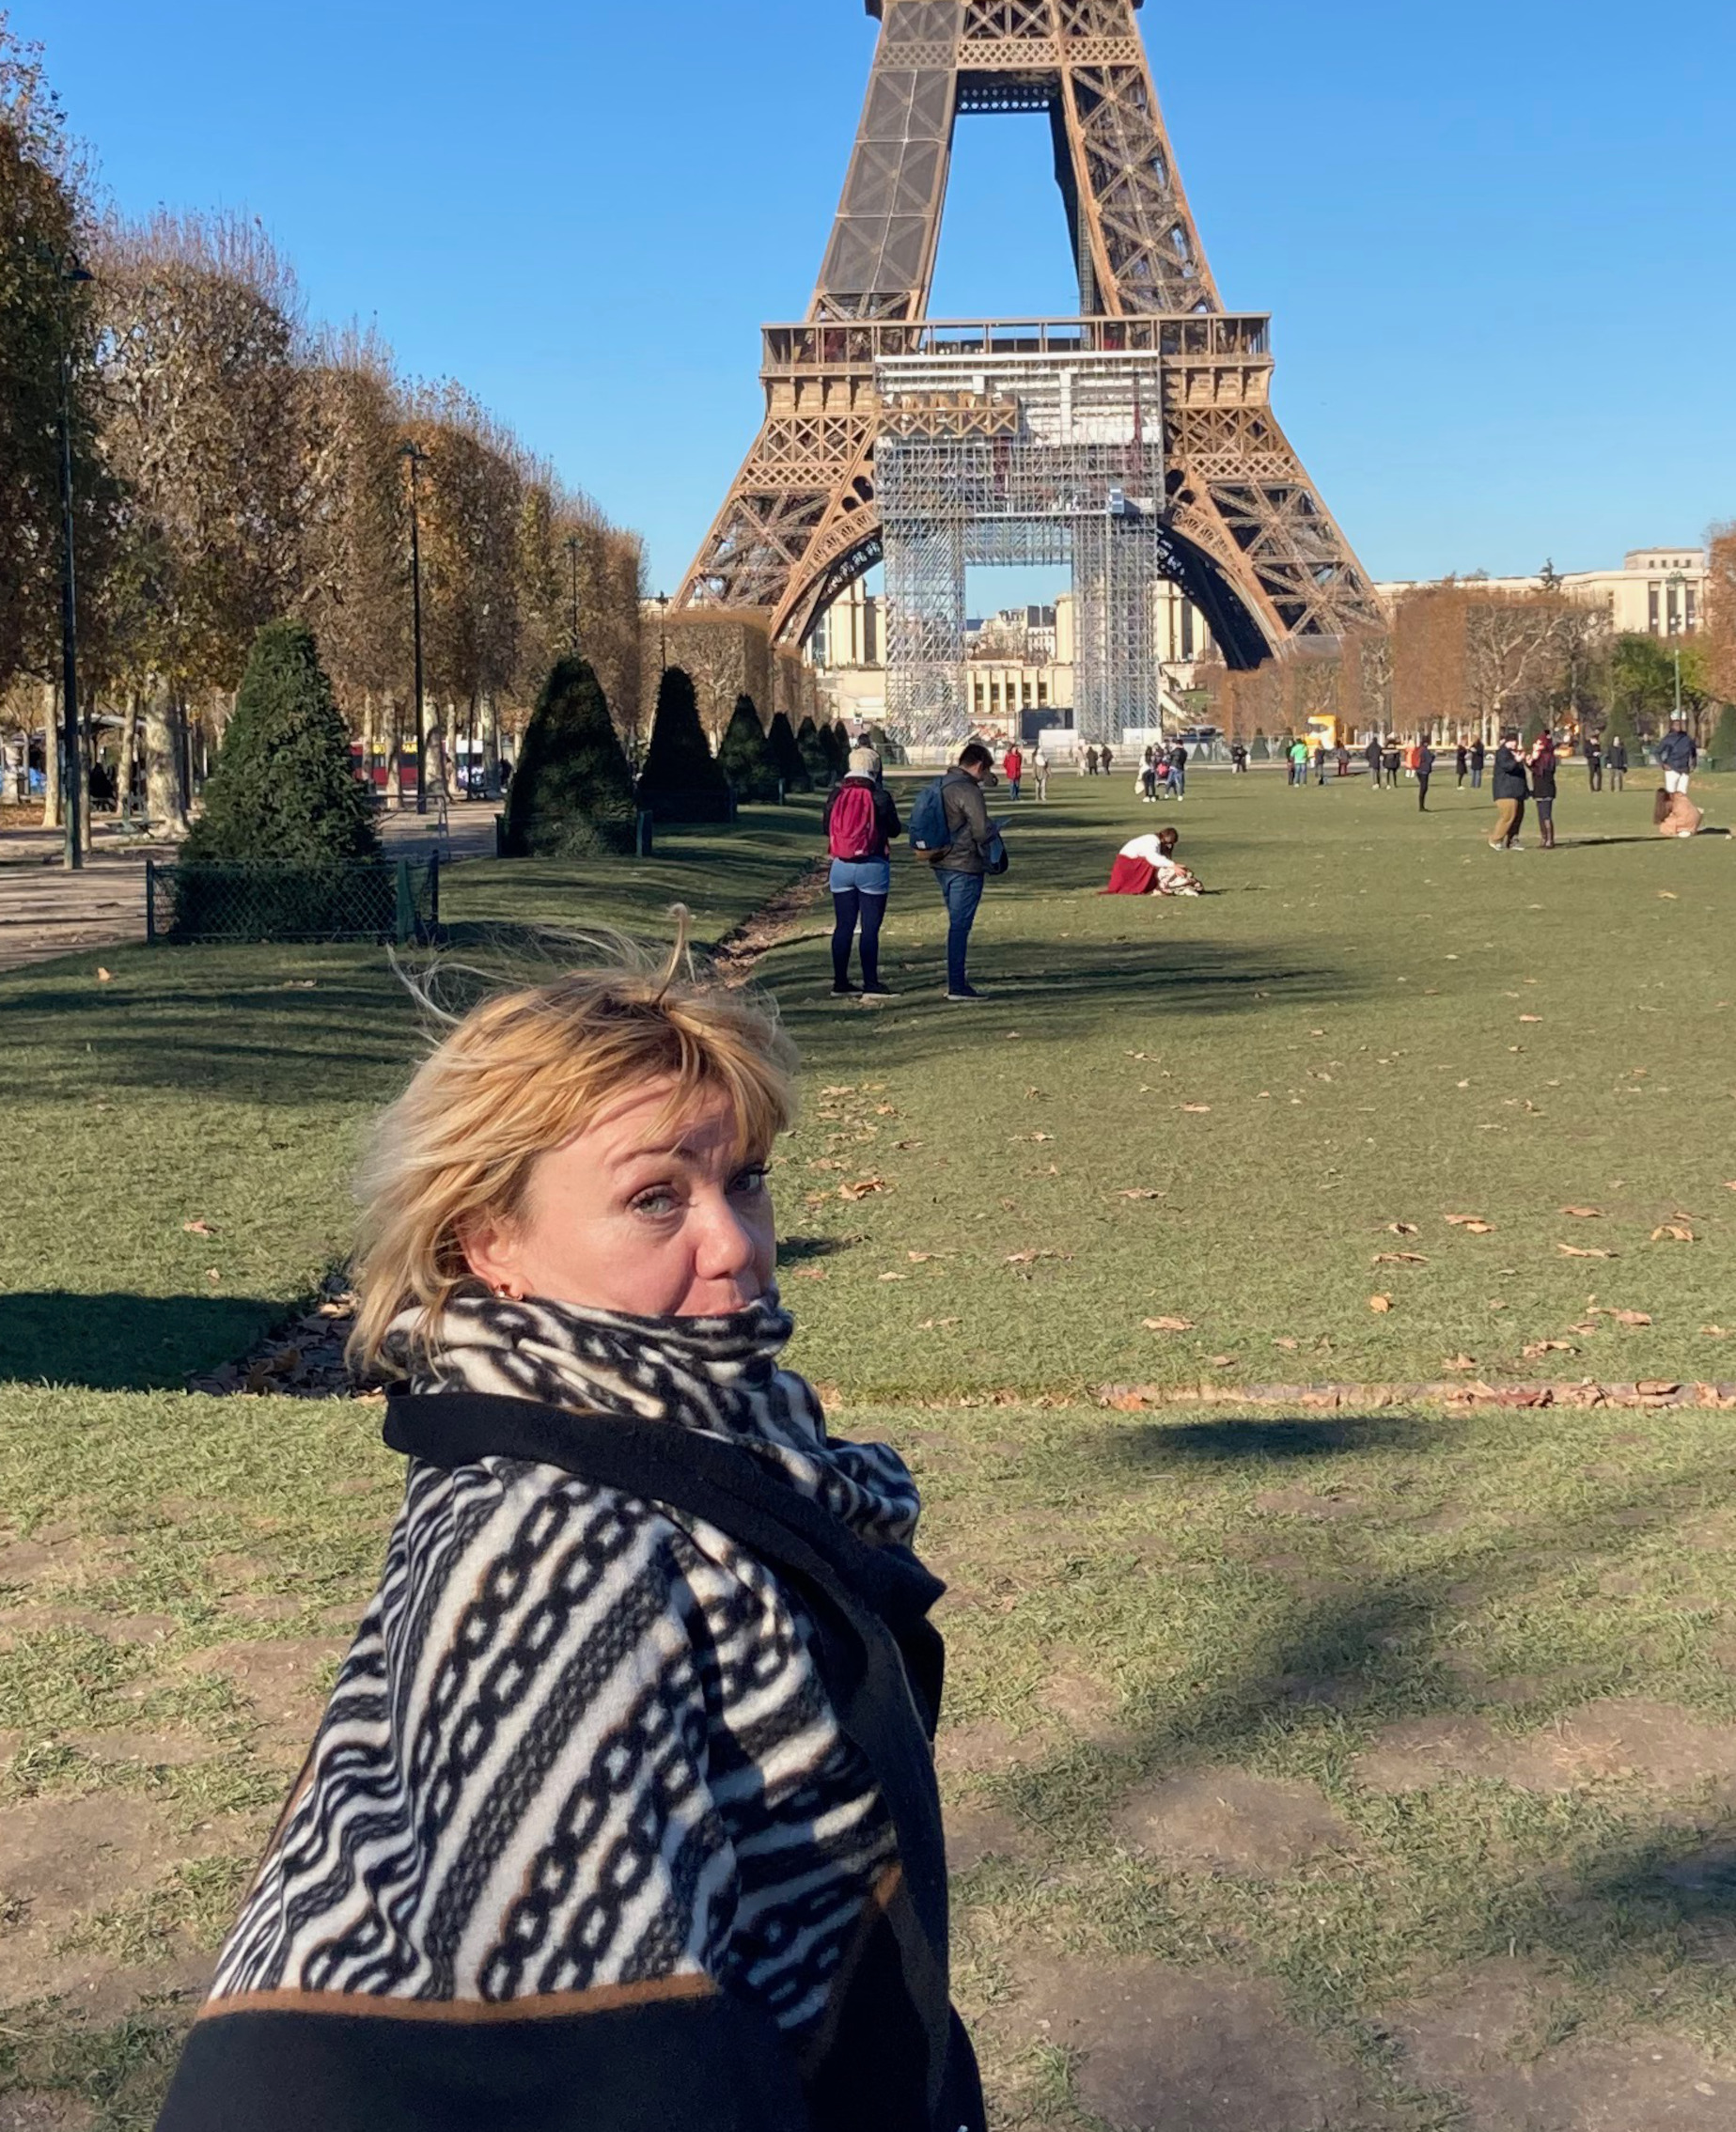
\includegraphics[height=14cm]{Rasa} \newline*1969-07-13 †2022-12-21}

\begin{document}
\isodate
\titlehead{
\includegraphics[height=4cm]{Logo_gross}}
\author{Thomas Thrien\\(thomas.thrien@tquadrat.org)}
\title{Extended Coding Conventions for Java}
\subtitle{Coding and Formatting Guidelines, Recommendations and Best Practices}
\date{\today}
\maketitle
\tableofcontents

\chapter{Introduction}\label{sec:Introduction}
To get your “Coding Guardrails for Java in a Nutshell”\index{Coding Guardrails for Java in a Nutshell}, you can take them from below:\footnote{obviously stolen from the “Zen of Python”\autocite{WIKIPEDIA:ZenOfPython,PYTHON_ORG_MAILING_LIST:ThePythonWay}\index{Zen of Python} and slightly amended~…}
\begin{enumerate}[nosep]\label{lst:NutshellGuardrails}
	\item{Beautiful is better than ugly.}\label{lst:ZoP:BeautifulVsUgly}
	\item{Explicit is better than implicit, and verbosity is your friend.}\label{lst:ZoP:ExplicitVsImplicit}
	\item{Do not repeat yourself.}\label{lst:ZoP:DRY}
	\item{Simple is better than complex.}\label{lst:ZoP:SimpleVsComplex}
	\item{Complex is better than complicated.}\label{lst:ZoP:ComplexVsComplicated}
	\item{Flat is better than nested.}\label{lst:ZoP:FlatVsNested}
	\item{Sparse is better than dense.}\label{lst:ZoP:SparseVsDense}
	\item{Readability counts.}\label{lst:ZoP:Readablity}
	\item{Special cases aren't special enough to break the rules~…}\label{lst:ZoP:SpecialCases}
	\item{…~although practicality beats purity.}\label{lst:ZoP:Practicality}
	\item{Errors should never pass silently and Exceptions may never be swallowed~…}\label{lst:ZoP:ErrorsMayNeverBeSwallowed}
	\item{…~unless explicitly silenced.}\label{lst:ZoP:ErrorsAreSilenced}
	\item{In the face of ambiguity, refuse the temptation to guess.}\label{lst:ZoP:DontGuess}
	\item{There should be one – and preferably only one – obvious way to do it~…}\label{lst:ZoP:OneWay}
	\item{…~although that way may not be obvious at first.}
	\item{Now is better than never~…}\label{lst:ZoP:Now}
	\item{…~although never is often better than \textit{right now}.}\label{lst:ZoP:RightNow}
	\item{If the implementation is hard to explain, it's a bad idea.}\label{lst:ZoP:BadIdea}
	\item{If the implementation is easy to explain, it may be a good idea.}\label{lst:ZoP:GoodIdea}
	\item{Without the unit test, it is not complete.}\label{lst:ZoP:NotCompleteWithoutTest}
	\item{Think about your future self and add a comment.}\label{lst:ZoP:FutureSelf}
	\item{Always do it right in the first place!}\label{lst:ZoP:BasicRule}
	\item{Have Fun!}\label{lst:ZoP:HaveFun}
\end{enumerate}

\section{The Goals}
The main goal of coding conventions in general is to help you writing better code.

So what is good code?

\paragraph{Good Code} does not have bugs and is running fast, without wasting valuable resources.

“Does not have bugs” also means that the code is doing what it is intended to do. We all know that it is nearly impossible to produce completely bug free code, for several reasons. An important reason is that already the specification, used as the base for the implementation, is often faulty. So the code is doing what it should do according to the specification, but it is not doing what it is meant to do~…

However, we should not forget that there is still the possibility for \textit{real} bugs.

And often you see the situation that your code is getting slower and slower, or is eating up more CPU cycles and/or memory than available. That may be due to higher data volumes or more users or lots of other reasons.

But as a result, you will have to modify your code – although, in most cases, it will be someone else who have to dig into \textit{your} code.  Or you are the unlucky one who needs to revise someone else's code.

So what you want is code that helps you with being modified – you want to have \textit{maintainable code}.

\paragraph{Maintainable Code}\index{maintainable code} supports its modification in various ways.

From a magazine dealing with software development tools, I found the following statement\footnote{I noted down the statement, but forgot to note the source – so if you know that source, I would appreciate if you would share it with me.}:

\begin{quotation}
“If you compare software development with the Apollo program, most programmers would be very successful bringing man to the moon, but never will get them back alive because of their common incapability to deliver software that can be maintained over a longer period of time with reasonable costs.” \\
\autocite{UnknownSource1}
\end{quotation}

Maintainability has a lot of facets, and I will discuss several of them in the run of this document. But before you can even think of modifying the code – either for fixing a bug, optimising the memory consumption, or adding new functionality – you need to identify the location.  

For that you have to read the already existing code, and of course, you have to understand what you are reading. So a crucial quality of maintainable code is that it is easy to read and \textit{basically} understandable\footnote{Ok, the requirement should be ‘easy to understand’, but that is a relative term. If something is ‘easily’ understandable depends from the experience level of the reader, and here we talk not only about their coding experience, but also about their familiarity with the problem domain. And you cannot always code for the rookies}.

No matter whether your code will meet all the other criteria that would make it maintainable: if it is not readable, it is not really maintainable. 

\paragraph{Readable Code}\index{readable code} can be easily consumed by a human.

\begin{quotation}
“[…], programs must be written for people to read, and only incidentally for machines to execute.”\\
Herold Abelson et. al.: \textit{Structure and Interpretation of Computer Programs}
\autocite{Sussman:StructureAndInterpretationOfComputerPrograms}
\end{quotation}

\begin{quotation}
“Everybody can write code that can be read by a computer, but only good developers will write code that can be read by humans.”\footnote{I agree in general, but also the converse is true: only developers that will write code that can be read by humans are good developers.} \\
Martin G. Fowler: \textit{Refactoring: Improving the Design of Existing Code}\autocite{Fowler:Refactoring}
\end{quotation}

Reading code is more important than writing code.\autocite{Marks:LocalVariableTypeInference:ReadingIsMoreImportantThanWriting}

Code is read much more often than it is written. Shorter programs can be preferable to longer ones, but shortening a program too much can omit information that is useful for understanding the program. The central issue here is to find the right size for the program such that understandability is maximized.

You should be specifically unconcerned here with the amount of keyboarding that is necessary to input or to edit a program. While concision may be a nice bonus for the author, focusing on it misses the main goal, which is to improve the understandability of the resulting program.

And from my experience I found that verbosity is your friend!\footnote{Refer to the “Coding Guardrails”, bullet point \ref{lst:ZoP:ExplicitVsImplicit}.}

Several guidelines and recommendations in this document, in particular regarding how to apply comments and how to write comments, but also those about to write a method, do require significant additional typing. Java in general has the reputation to be too verbose, and this coding conventions will even add to that verbosity – but as said: that's not generally bad!

But if you are afraid of the keyboarding, you should learn typewriting! For my understanding, someone who does not reach at least 100~CPM\footnote{CPM = “Characters per minute”, or, in German: „Anschläge pro Minute“} should look for a job outside of software development!\footnote{Average values for a trained typist are around 200 CPM, peak values are at 500 to 900 CPM.}

Writing code is not the only area where you would benefit from mastering that important skill; it will also help you to write all the other stuff you have to deliver in addition to your code (documentation, meeting notes, emails, specification documents,~…).

Also, modern IDEs do a lot of the typing for you, as long as you take the trouble to configure them appropriately. Refer to chapter \tqfullref{sec:ToolSupport}.

Code readability shouldn’t depend on IDEs.\autocite{Marks:LocalVariableTypeInference:NoIDEDependency}

Code is often written and read within an IDE, so it is tempting to rely heavily on the code analysis features of IDEs. Unfortunately, code is at least as often read \textit{outside} an IDE. It appears in many places where IDE facilities are not available, such as snippets within a document, browsing a repository on the internet, or in a patch file. It is counterproductive to have to import code into an IDE simply to understand what the code does.

Code should be self-revealing. It should be understandable on its face, without the need for assistance from tools.

\subsection{Conclusion}
To summarize from above, the goal for these coding conventions is to help you to write~…
\begin{itemize}[nosep]
	\item …~good,~…
	\item …~maintainable,~…
	\item …~readable~…
\end{itemize}
…~Java source code.

As a side effect, all source code looks familiar to all members of the team. That conformity supports readability, but such a common look also identifies the source code as written by the team, as its trademark.

\section{About this Document}
This document was compiled using \TeX/\LaTeX\index{TeX}\index{LaTeX}\footnote{In case it is relevant for you, I used ‘TexMaker’ as the editor for the \LaTeX~sources. I run it on Mac and Linux, but the software is also available for Windows; it can be downloaded from this location: \url{https://www.xm1math.net/texmaker/download.html}.}, and its source can be found on GitHub\autocite{TQUADRAT_ORG_DOCUMENT_REPOSITORY}\index{github}. The diagrams were generated with Graphviz\index{graphviz}.

\subsection{The Document Structure}
This document itself consists of four major parts, aside of this \nameref{sec:Introduction} and the \nameref{sec:Appendices} (containing additional information, references and examples).

\paragraph{\nameref{sec:FormattingTheSourceCode}} deals with proper formatting of the Java source files additional files that are part of your project.

\paragraph{\nameref{sec:NamingConventions}} covers the naming of the program elements (modules, packages, classes, methods, fields, local variables, formal parameters).

\paragraph{\nameref{sec:WritingProperComments}} discusses some guidelines for writing proper comments.

\paragraph{\nameref{sec:CodingGuidelines}} is the biggest part and provides guidelines on how to use various language features, based on best practices.

\subsection{Sample Code}
The code samples in this document underline some particular aspect or demonstrate a single guideline or recommendation; to stay focused on that purpose, and to keep the samples at a reasonable length, they may often hurt other guideline or ignore other recommendations. For instance, in most cases, methods are lacking the required comments, the names are not really meaningful, or mandatory error handling is just missing.

The source code samples in chapter \tqfullvref{sec:Examples} obey all rules, follow all guardlines and implement all recommendations.

All the rules, guidelines and recommendations in this document assume that you use at least Java~17\footnote{see the language specification in \autocite{ORACLE_DOC_LANGUAGE_SPECIFICATION}} to write and to compile your code. I used that version also for the samples.

\subsection{References}
Instead of adding URLs directly into the document, I provided them in the “Bibliography” section. In the text, you will find references to it like this: \autocite{ORACLE_DOC_LANGUAGE_SPECIFICATION}. If you read the electronic version of the document, the reference is clickable and brings you to the respective entry. There you can click on the URL.

This allows me to update the URLs on one single location if they will change. 

\section{History and Implementation}
Around the year~2000 I was asked to compile a set of coding guardrails for a team of developers that had been new to Java (and most were new to programming, too). That was the very first version of this document, based on the “Code Conventions for the Java\textsuperscript{TM} Programming Language”\autocite{SUN_CODE_CONVENTIONS} and the way I wrote Java code at that time.

Later versions were created for other developer teams, and several software projects had been delivered successfully working with these coding conventions.

Some of the code from these projects is still alive, proving the initial statement that coding conventions do help to create maintainable software.

I wrote a lot of code using the rules, guidelines and recommendations from this document (and its predecessors, of course), including some libraries that I published on GitHub. Some of the code from these libraries is mentioned in chapter \tqfullref{sec:CodingGuidelines}, starting on page~\pageref{sec:CodingGuidelines}, I also added some stuff as examples in chapter \tqfullref{sec:Examples} in the “\nameref{sec:Appendices}” chapter. If you are interested in the whole package, you should have a look to \autocite{TQUADRAT_ORG}.

\section{Other Programming Languages}\label{sec:OtherProgrammingLanguages}
Of course coding conventions like those described with this document are not only useful for Java programs, but for code in any other programming language also.\footnote{Even for descriptive languages like XML and HTML they make sense, also for documents written in \TeX/\LaTeX.} But each language has its unique features and specialities, meaning that coding conventions written for one programming language do not necessarily match the requirements for another.

Obviously there are some common rules that are valid for every programming language\footnote{E.g. the request to use meaningful names.}, but usually the differences will outweigh the similarities. So it is not a good idea to do something in language \verb#A# just and only it is done that way in language \verb#B#. On the other side, it should always be proved whether something that worked fine for one language would not be a great idea to be applied to code in another language, too.

In this sense, I stole the “Zen of Python”\autocite{WIKIPEDIA:ZenOfPython,PYTHON_ORG_MAILING_LIST:ThePythonWay}\index{Zen of Python}\footnote{I added the ellipsis.} and used it for this document:

\begin{itemize}[nosep]
	\item Beautiful is better than ugly.
	\item Explicit is better than implicit.
	\item Simple is better than complex.
	\item Complex is better than complicated.
	\item Flat is better than nested.
	\item Sparse is better than dense.
	\item Readability counts.
	\item Special cases aren't special enough to break the rules~…
	\item …~although practicality beats purity.
	\item Errors should never pass silently~…
	\item …~unless explicitly silenced.
	\item In the face of ambiguity, refuse the temptation to guess.
	\item There should be one – and preferably only one – obvious way to do it~…
	\item …~although that way may not be obvious at first unless you're Dutch.
	\item Now is better than never~…
	\item …~although never is often better than \textit{right now}.
	\item If the implementation is hard to explain, it's a bad idea.
	\item If the implementation is easy to explain, it may be a good idea.
	\item Namespaces are one honking great idea – let's do more of those!
\end{itemize}

Only the last one regarding “Namespaces” does not work for code written in Java, unless you translate “Namespace” to “Package” (or “Module”~…).

A good example for the other way round – other programming languages adopting a feature from Java – is the idea to add documentation comments to the source code and to use a tool like JavaDoc\index{javadoc} to externalise them and publish them as the API documentation. It was adopted for various other languages, including so different specimen as C/C++, JavaScript and PL/SQL.\footnote{Although I have to confess that the commenting style is not part of the specification of these languages but only supported by external tools; one of these tools is doxygen\autocite{DOXYGEN_HOMEPAGE}\index{doxygen}.} Obviously, if you want to benefit from that adopted feature, you have to write your C++ (JavaScript, PL/SQL,~…) code (more precise, your documentation comments) according to coding conventions similar to those defined here.

A sample for code conventions for JavaScript can be found in the web at \autocite{Crockford:JAVASCRIPT_CODE_CONVENTIONS}.

Coding conventions for C\# are part of Microsoft's documentation for C\#\autocite{MICROSOFT:CsharpDocumentation}, another source can be found on GitHub\autocite{Taranov:CsharpCodingStandards}.

The number of documents dealing with coding standards, naming conventions and style guides for C++ is close to infinite. A starting point could be the ISO page\autocite{ISO:CppCodingStandards} or Google's C++ Style Guide\autocite{Google:CppStyleGuide}.

\section{Code Generators}
Java code that is automatically generated by another piece of software should implement this coding conventions in the same way as “hand crafted” code. Most generators are highly configurable and/or allow to use code templates that are customisable.\footnote{Perhaps you want to have a look to \autocite{TQUADRAT_ORG_FOUNDATION_JAVACOMPOSER}.}

Especially if base classes will be generated it is important that proper comments are generated at least for all API elements; this covers all \lstinline|public| and \lstinline|protected| elements, and in some cases all package-local elements, too.

Java~6 introduced an annotation \lstinline|javax.annotation.Generated|\index{javax.annotation!Generated} (\lstinline|@Generated|) that should be used to mark generated code. Refer to \autocite{ORACLE_DOC_GENERATED_ANNOTATION} for the details.\footnote{In case you still have to use Java~5 as the source code version, you should consider to create your own \lstinline|@Generated| annotation along the lines given by that existing implementation in Java~6 and later.}

\section{Coding for Sustaining}\label{sec:CodingForSustaining}
And what to do with “legacy” code that has to be fixed, amended or extended? 

Most probably that code will not follow \textit{these} coding conventions (if any at all~…), and it is rarely a good idea to reformat or completely rewrite the existing source code just to align it with the current recommendations and guidelines. Instead a fix should be limited to that area in the source code that is broken.

But if possible, your fix should incorporate the standards defined by this document. Be creative how to implement these standards. So if a method has to be reimplemented completely, format it as described here and add the appropriate JavaDoc comments\footnote{Even when there are no other JavaDoc comments in the whole file~…}, if missing. Or if a new field has to be added to a class, add the “\verb#m_#” prefix to its name (see chapter \tqfullref{sec:Fields}).

Obviously, completely new interfaces and classes should be implemented fully compliant to this conventions.

In this context, see also chapter \tqfullvref{sec:MaintenanceComments}.

\section{Tool Support}\label{sec:ToolSupport}
Several of the rules, guardrails and recommendations in this document can be implemented through the configuration of the programming enviroment that is used, especially those from chapter \tqfullref{sec:FormattingTheSourceCode} that deals with the formatting of the source code.

The chapter \tqfullref{sec:IDEConfiguration} provides some configuration samples for Eclipse and JetBrains IntelliJ IDEA.

\section{How to use this Document?}\label{sec:HowToUseThisDocument}
First, you can use this document as is! It should work for you, as its predecessors already worked for a bunch of project teams.

But you can also shape it closer to your particular needs, if you want! As said, you find the sources for this document on GitHub. Clone the repository on GitHub \autocite{TQUADRAT_ORG_DOCUMENT_REPOSITORY}, replace the examples and the references to my libraries by some that fits better to your project and/or your company, then adjust the other stuff accordingly.

In particular, for your project, you should elaborate on the following topics:
\begin{itemize}
	\item{Chapters \tqfullvref{sec:Projects}, \tqfullvref{sec:Modules}, \tqfullvref{sec:Packages} and \tqfullvref{sec:LibraryFiles}\\
	In no particular order:
	    \begin{itemize}
		    \item{Specify the name of your project.}
		    \item{Specify a format for the names of the library file(s) produced by your project.}
		    \item{Specify the names for the modules and packages of your project.}
	    \end{itemize}}
	
	\item{Chapters \tqfullvref{sec:Logging} and \tqfullvref{sec:LoggerConfiguration}:
	    \begin{itemize}
		    \item{Specify the type of the logging framework you use in your product – if any – or if you want to code against SLF4J (or if you do not want to log at all).}
		    \item{Specify the names of the loggers.}
		    \item{Specify the format for the log messages, in particular for the log levels \verb#DEBUG# and \verb#TRACE# (or \verb#FINE#, \verb#FINER# and \verb#FINEST#, if you are using JDK~Logging).}
		    \item{Provide a (default) logging configuration.}
		    \item{Optionally, you may remove all references to the logging frameworks and APIs that you do \textit{not} use in your project.}
	    \end{itemize}}
	    
	\item{Chapter \tqfullvref{sec:TheNamingDictionary}:
	    \begin{itemize}
		    \item{Add verbs that are specific to your project, remove obsolete/unwanted ones.}
		    \item{Adjust the description for verbs where appropriate.}
		    \item{Do the same for the class name suffixes.}
		    \item{Add a Glossary that explains special terms used in the context of your project (the “Domain Specific Terminology”).}
	    \end{itemize}}
	
	\item{Chapter \tqfullvref{sec:IDEConfiguration}:
	    \begin{itemize}
		    \item{Remove the configuration setting samples for the IDEs that you are not using.}
		    \item{Adjust the configuration setting sample according to the changes you made elsewhere.}
		    \item{Add matching configuration setting samples for additional IDEs used in your environment.}
	    \end{itemize}}
	
	\item{Provide code snippets for recurring patterns that are specific to your project.}
	
	\item{Remove this chapter \tqfullref{sec:HowToUseThisDocument} and the chapter \tqfullref{sec:HowToImplement}.}

\end{itemize}

\section{How to implement these ‘Coding Conventions’ in your Project?}\label{sec:HowToImplement}
First any coding conventions are better than none! So if your team is already adhering to some coding conventions, the first hurdle had been taken already.

Adjust this document that it will incorporate the already accepted guidelines and recommendations; this may require that you remove conflicting recommendations and guidelines – don't care, just do it!

The biggest blocker in this case could be that too much code needs to be modified to match with the coding conventions, meaning tedious work no one likes to do. In this regard, you should also have a look to the chapter \tqfullvref{sec:CodingForSustaining}.

But the most simple case is a new team starting over with a new project from scratch. Just present the document as is~…

Experienced programmers know about the benefits of having detailed guard\-rails they can follow – in particular when they know that the other team members will also follow the same guardrails.

Nevertheless, you may have one or the other hacker in your team that complains that this kind of guardrails are suffocating their creativity.

Perhaps this helps: I was always interested in fotography, and therefore I attended some classes about the topic. There the question was raised what are bad pictures, good pictures and exceptionally artistic pictures, and the professor explained it like this: Fotography has a whole bunch of rules on how to compose a good picture, and you do not even need to know one of these rules to distinguish a bad shot from a good fotography: the bad ones will break the rules.

But the really artistic pictures always break \textit{one} or \textit{the other} rule, but \textit{with intention}. The fotographer's creativity is to choose the rule to break and how – but this first means that they have to know each of the rules and how to follow them (usually referred to as ‘knowing the craft’), and second, that there is a visible intention.

But in most cases the client just wants to get only good pictures.

Same in software development: only few clients pay for a piece of art; instead they expect good craftsmanship.

If this explanation does not help, and you are in the proper position: replace the hacker.

\section{About the Author}
My name is Thomas Thrien, I was born and raised in Germany, still live there, so my primary language is German, not English. You may notice that one or the other time when you read this text: although I have to speak English most of time on the job, I too often fall back to Denglish~…

I am in the IT business since 1982 now, mainly in roles dealing with support, field service, and sustaining, but over the years I also did some development work, and even some IT consulting. I did the ground work with my fingers on the keyboard as well as leading teams of various size, even running whole departments.

But in support and sustaining, you are mainly on the “receiving end” of the development process, suffering from the output of development teams that had never heard about the basics, or don't care about them. This experience was my main motivation to compile this document, and to keep it up to date.
 
If you have questions or comments regarding this document, please send me an email to \href{mailto:thomas.thrien@tquadrat.org}{thomas.thrien@tquadrat.org}. Or leave it at \url{https://tquadrat.github.io/}.

\section{The Basic Rule}\label{sec:TheBasicRule}
One rule should be followed before any other rule or recommendation given in this document, that one listed as bullet point~\ref{lst:ZoP:BasicRule} in the nutshell version of the \hyperref[lst:NutshellGuardrails]{“Coding Guardrails for Java”}:\footnote{And it does not contradict with bullet points~\ref{lst:ZoP:Now} and \ref{lst:ZoP:RightNow}!}

\begin{center}
	\begin{huge}
		\fbox{\textbf{Always do it right in the first place!}}
	\end{huge}
\end{center}

Experiences with lots of programming projects have shown that programmers seldom touch their code again, once it is written.\footnote{Usually, they will return to the code only when it is broken – and then they want to fix the bug as fast as possible, not adding missing comments or reformatting the code~…} As a result, missing comments will never be added, shady programming patterns would not be fixed – with the consequence that in case of a bug the maintainer is lost in a poorly documented chaos of badly formatted source code.

\textit{And this is exactly what we want to avoid!} 

This means there is never ever any excuse for omitting comments, using ‘temporary’ names or doing other ‘funny’ things. And we all know about all the quick and dirty PoCs that made it into a product without significant changes to the code~… – treat a PoC in the same way as product code.\footnote{I was inclined to add “There is nothing like a \textit{disposable prototype}.” to the \ngref~…}

Of course you can interpret this also as “Don't make mistakes”, but we all now that humans make mistakes, and that it is unavoidable that our code will contain one or the other bug. So it means that you should \textit{do your best} to avoid mistakes, and the rules, guidelines and recommendation from this document will help you with that.

So again:

\begin{center}
	\begin{huge}
		\fbox{\textbf{Always do it right in the first place!}}
	\end{huge}
\end{center}

But the most important rule from the \ngref{} is that with the bullet point number~\ref{lst:ZoP:HaveFun}:

\begin{center}
	\begin{huge}
		\fbox{\textbf{Have fun!}}
	\end{huge}
\end{center}

%------------------------------------------------------------------------------

\chapter{Formatting the Source Code}\label{sec:FormattingTheSourceCode}
As said already coding conventions are primarily guidelines that should help making code better to maintain. Usually, this starts with making it better readable.

In this regard, a source file is like any other text document, it benefits from having a clear structure, and that structure is supported by the formatting of the text.

An article may have sections with headlines in bold face, the paragraphs are separated by blank lines and the first lines of them are indented by 0.3~cm, and there are rules about line length and hyphenation.

This chapter deals with the proper formatting of source files and their structure with the goal to get readable \textit{documents}.

\begin{quotation}
“[…], we want to establish the idea that a computer language is not just a way of getting a computer to perform operations but rather that it is a novel formal medium for expressing ideas
about methodology.”\\
Herold Abelson et. al.: \textit{Structure and Interpretation of Computer Programs}
\autocite{Sussman:StructureAndInterpretationOfComputerPrograms}
\end{quotation}

\subsubsection{Principles}
\begin{enumerate}[label=P\arabic*.]
	\item{The structure of the program text must support the flow of reading.
	
	As said in the \ngref, bullet point~\ref{lst:ZoP:Readablity}: “Readability counts”.}
	
	\item{The formatting of the program text has to be consistent.
	
	Permanent changes in the way things are written will confuse the reader.}
	
	\item{Navigation through the source file should be easy.
	
	When loaded inside an IDE, navigating inside a Java source file is easy: click on the name of the respective program element and the cursor is moved to the corresponding line in the file.
	
	But when using a plain text editor, the search function is often the only tool you have. A consistent structure with headlines and a defined order would help here, too.}
	
	\item{It does not harm when the source code also looks beautiful.
	
	Bullet point~\ref{lst:ZoP:BeautifulVsUgly} from the \ngref~ is also about the visual appearance of the source code. We can discuss how useful ASCII art in a source file is, but not that it can contribute to the beauty of the program text.}
\end{enumerate}

\section{Indentation}\label{sec:Indentation}
Indentation\index{indentation}, together with empty lines, is the most important tool to structure any source code.

\subsection{Indentation Style}\label{sec:IndentationStyle}
For most programming languages, the indentation of code blocks increases the readability – for others, like Python\autocite{W3SCHOOLS:PythonIndentation}, the indentation is even part of the syntax rules.

Obviously, “readability” is a relative term, depending from one's habits. So some people are more familiar with the Kernighan-Ritchie (K\&R) indentation style\index{Kernighan-Ritchie style}\index{K\&R style|see{Kernighan-Ritchie style}}

\begin{lstlisting}
public final void myMethod (){
    if (flag) {
        …
    }
}   //  myMethod()
\end{lstlisting}

as it is also shown in the “Code Conventions for the Java\textsuperscript{TM} Programming Language”\autocite{SUN_CODE_CONVENTIONS}, other prefer to have the curly braces on a line of their own (sometimes referred to as GNU or BSD style\index{GNU style}\index{BSD style}\footnote{All, BSD, GNU and K\&R styles, will define more than just how to place the curly braces. In addition, all three are originally part of code conventions for programming in C and/or C++ that cannot applied to Java without modifications. See chapter \tqfullvref{sec:OtherProgrammingLanguages} on this topic.}):

\begin{lstlisting}
public final void myMethod()
{
    if( flag )
    {
    	…
    }
}   //  myMethod()
\end{lstlisting}

Both styles will work, but they look different. So as a lot of other guidelines from a code conventions document, too, this is a matter of taste. But as conformity suppports readability, a main purpose of these guidelines is to ensure that all source code looks similar, and we have to determine the style to use.

I prefer the so-called GNU or BSD style\index{indentation!style} and recommend it to you as well, because it makes it easier to detect the begin and the end of a code block than the Kernighan-Ritchie style. It demands to have the opening and closing curly braces on a line of their own, like this:

\begin{lstlisting}
public final class MyClass
{
    public final void myMethod()
    {
        if( flag )
        {
            /* do something */
        }
        
        for( final var i = 0; i < max; ++i )
        {
            /* do something else */
        } 
    }   //  myMethod()
}   //  class MyClass
\end{lstlisting}

\subsection{Indentation Size}\label{sec:IndentationSize}
Again, at the very end, the size for the indentation is a matter of taste. But using four (4) spaces\index{indentation!size|see{indentation!base unit}}\index{indentation!base unit} has been established as a de~facto standard for the base unit of indentation in Java source code, also because the original Sun Code Conventions\autocite{SUN_CODE_CONVENTIONS:Indentation} stated it that way. Therefore I recommend that you also use four spaces (\lstinline|' '|, ASCII~32 or 0x20) as the base unit of indentation.

When you write code \textit{snippets} for a publication (for an article, as part of a program documentation, or for an answer on StackOverflow\autocite{STACKOVERFLOW}~…), sometimes using a base indentation unit of two spaces would be better, as it spares some room. But reformatting existing code for this use case is in most cases not worth the effort.

\subsection{Indentation Character}\label{sec:IndentationCharacter}
As said, you should use four \textit{blanks}\index{indentation!character}; do \textit{not} use tabs (\lstinline|'\t'|, ASCII~9 or 0x09)! Tabs are \textit{not} allowed! This is different from the Sun Code Convention\autocite{SUN_CODE_CONVENTIONS:Indentation} that do not explicitly specify whether to use blanks or tabs.

Usually both, the indentation character and the indentation base unit can be configured in your IDE; in Eclipse this is part of the \textit{Formatter} definition (\verb#Window|Preferences|Java|Code Style|Formatter#).

%------------------------------------------------------------------------------

\section{White Space}
This chapter deals with the white space other than the indentation blanks.

\subsection{Blank Lines}\label{sec:BlankLines}
Blank lines improve readability by setting off sections of code that are logically related.
If not separated by an explicit comment, a blank line should always be used in the following circumstances:
\begin{itemize}
\item{Between parts of a class declaration\footnote{Although this would hurt the guidelines for commenting as set in chapter \tqfullref{sec:StructuringComments}}}
\item{Between class and interface definitions}
\item{Between methods}
\item{Before a block or single-line comment}
\item{Between logical sections inside a method to improve readability}
\item{To group some code lines logically}
\end{itemize}

More than one blank line should be avoided, but if it seems feasible for a particular purpose, feel free to use ASCII art to express the separation of parts in the source file.

This is again different from what the Sun Code Conventions\autocite{SUN_CODE_CONVENTIONS:BlankLines} stated.

\subsection{Parenthesis}\label{sec:Parenthesis}
Parenthesis are of course no whitespace characters – in the opposite, they are important syntax elements. But they trigger the use of whitespace, in particular blank spaces, and therefore, they are mentioned in this chapter.

We distinguish between \textit{arithmetical} parenthesis and \textit{parameter} parenthesis; the first is used in (mathematical or logical) expressions to order the terms, the latter is used with method or constructor calls or in lambdas.

The Sun Code Conventions\autocite{SUN_CODE_CONVENTIONS:BlankSpaces} does not make this distinction, and it handles them differently (in the same way as arithmetical parenthesis).

\paragraph{Arithmetical Parenthesis}
An opening arithmetical parenthesis is always \textit{preceded} by a blank or another opening parenthesis and \textit{never} followed by a blank. A closing arithmetical parenthesis is \textit{never preceded} by a blank, but \textit{always followed} either by another closing parenthesis, a blank, or a newline (or a semicolon, in case the statement ends).

\paragraph{Parameter Parenthesis}\label{sec:ParameterParenthesis}
An opening parameter parenthesis is \textit{never preceded} by a blank and \textit{ever followed} by one, while a closing parameter parenthesis is \textit{always preceded} by a blank. The only exception is for empty arguments lists where the opening parenthesis is immediately followed by the closing parenthesis.

Of course this is also valid for the declaration of methods and constructors.

Regarding to this rule, \lstinline|if|, \lstinline|for|, \lstinline|while|, \lstinline|try| and \lstinline|switch| are treated like they are functions.\footnote{And also the keywords \lstinline|catch| and \lstinline|synchronized|, but they do not allow complex terms inside their 'argument list'.}

This rule can improve the readability of complex terms drastically, as the examples below will illustrate.

\begin{lstlisting}[numbers=left]
final int v = (a + b) * 5;
final double d = sin( (a + b) / c );

System.out.println( "Finished!" );
set( get() );
System.out.println( sin( ((a + b) * (c + 4) + c)) / d ) );
if( a < b ) c = (d + e) / sin( f );
while( ((line = reader.readLine()) != null) && (++i < capacity) )
    processLine( line );
\end{lstlisting}

A special case are parenthesis used with a cast:
\begin{lstlisting}
final Object o = "Text";
final var s = (String) o;
\end{lstlisting}
Here an opening parenthesis is never followed by a blank, and a closing one is never preceded by a blank.

\subsection{Blank Spaces}\label{sec:BlankSpaces}
In addition to what was said already, blank spaces should be used in the following circumstances:
\begin{itemize}
\item{With a keyword followed by a parenthesis, like \lstinline|if|, \lstinline|while|, \lstinline|for| etc. There is no blank space between the keyword and the opening parenthesis, but  between that parenthesis and the argument. Another blank space is between the (last) argument and the closing parenthesis. As a short it can be said that parenthesis for these keywords will be treated like parameter parenthesis, as already stated in \tqfullref{sec:ParameterParenthesis}.\footnote{This is in opposite to the sun codeing conventions \autocite{SUN_CODE_CONVENTIONS}; there it is recommended to have a blank between the keyword and the opening parenthesis while not using it between the method name and the opening parenthesis here, just to distinguish between keywords and methods calls. I think that it is more important to distinguish between parenthesis in arithmetical expressions and those in method calls.}

Examples:
\begin{lstlisting}[numbers=left]
while( true )
{
    …
}

for( int i = 0; i < 10; ++i ) { … }

try
{
    …
}
catch( Exception e )
{
    e.printStackTrace();
}

if( list.isEmpty() ) { … }
\end{lstlisting}}
\item{A blank space has to appear after commas in argument lists. The exception are generics where the comma is not followed by a blank space in case there is more than one type.

Examples:
\index{java.util!Map}\index{java.util!HashMap}
\begin{lstlisting}[numbers=left]
Map<String,String> map = new HashMap<String,String>();
Map<String,String> map = new HashMap<>(); // using the diamond operator
map.put( key, value );
\end{lstlisting}}
\item{All binary operators except “\verb#.#” has to be separated from their operands by spaces. Blank spaces should never separate unary operators such as unary minus, increment (“\verb#++#”), and decrement (“\verb#--#”) from their operands.

Example:
\begin{lstlisting}[numbers=left]
a += c + d;
a = (a + b) / (c * d);

while( d-- > s++ )
{
    ++n;
}

printSize( "size is " + foo + "\n" );
\end{lstlisting}}
\item{The expressions in a \lstinline|for| statement has to be separated by blank spaces after the semicolon.

Example:
\begin{lstlisting}
for( expr1; expr2; expr3 )
{
    …
}
\end{lstlisting}

For an extended for loop, blank spaces has to be placed around the colon, too:
\begin{lstlisting}[numbers=left]
for( String s : stringArray ) System.out.println( s );
\end{lstlisting}}
\item{For ternary statements, the question mark (“?”) and the colon (“:”) has to be surrounded by blank spaces:

Example:
\begin{lstlisting}
int signum = d < 0 ? -1 : d > 0 ? 1 : 0;
\end{lstlisting}

In this sample, some parentheses would be helpful, too.}
\item{Casts should be followed by a blank space. 

Examples:
\begin{lstlisting}
myMethod( (byte) aNum, (Object) x);
myMethod( (int) (cp + 5), ((int) (i + 3)) + 1 );
\end{lstlisting}}
\end{itemize}

%------------------------------------------------------------------------------

\section{Line Length}\label{sec:LineLength}
Several sources (including the original Sun Code Conventions for the Java\textsuperscript{TM} Programming Language”\autocite{SUN_CODE_CONVENTIONS:LineLength}) recommend to avoid code lines longer than 80~characters, because they were not handled well by many terminals and tools.

This had been true at the time those documents were written\footnote{The “Code Conventions for the Java\textsuperscript{TM} Programming Language”\autocite{SUN_CODE_CONVENTIONS} were published in 1999~…}, but today's  graphical screens are much wider (sometimes even 200 and more characters can be put into one line), and modern tools do not even care about line length, so we do not want to recommend a fixed line length for source code.\index{line length}

\textbf{Note:} Sample code for the use in documentations, articles or alike should have a limited line length – generally not more than 70~characters.\index{line length!articles and documentation}

Different to that, comment lines are limited to 80~characters – or more precise, they have to end at column~80\index{line length!comments}. All lines with “ASCII graphics” are extended to that column. This is pertaining to the beginning comments (chapter \tqfullvref{sec:BeginningComment}), the structuring comments (chapter \tqfullvref{sec:StructuringComments}) and most single-line comments (chapter \tqfullref{sec:SingleLineComments}).

\subsubsection{Wrapping Lines}\label{sec:WrappingLines}
As we have an unlimited line length, it will not happen that an expression does not fit into a single line. But you should break long lines to improve the readability. In this case, you should follow these general principles:
\begin{itemize}
\item{Only one statement per line!}
\item{Break after a comma.}
\item{Break before an operator.}
\item{Break before a dot.}
\item{Break after an opening parenthesis and before a closing one.}
\item{Prefer higher-level breaks to lower-level breaks.}
\item{Align the new line with the beginning of the expression at the same level on the previous line.}
\item{If the above rules lead to confusing code or to code that's squished up against the right margin, consider to break up the code into multiple parts, by introducing additional temporary variables.}
\end{itemize}

Here are some examples of breaking method calls:
\begin{lstlisting}[numbers=left]
//  USUAL
final var result = myMethod( longExpression1, longExpression2, 
    longExpression3, longExpression4, longExpression5 );
        
//  SINGLE LINE FOR EACH ARGUMENT
myProcedure
( 
    longExpression1,
    longExpression2,
    longExpression3,
    longExpression4, // some comment
    longExpression5
);

final var result = myMethod
    ( 
        longExpression1,
        longExpression2,
        longExpression3,
        longExpression4, // some comment
        longExpression5
    );

//  OTHER VARIANTS
final var result = myMethod( longExpression1,
    someMethod( longExpression2,
        longExpression3 ) );

final var result = myMethod1( longExpression1,
    someMethod( longExpression2,
        longExpression3 ),
    longExpression4,
    otherMethod( longExpression5 ) );
\end{lstlisting}

Using a single line for each argument makes especially sense in cases where one or more expressions are really long, or if a comment should be added to the argument.

Next there are two examples of breaking an arithmetic expression. The first is preferred, since the break occurs outside the parenthesized expression, which is at a higher level.
\begin{lstlisting}[numbers=left]
// PREFERRED
final var longName1 = longName2 * (longName3 + longName4 - longName5)
    + 4 * longname6;
           
longName1 = longName2 * (longName3 + longName4 - longName5)
    + 4 * longname6;
           
// AVOID!!!           
longName1 = longName2 * (longName3 + longName4
                       - longName5) + 4 * longname6;
\end{lstlisting}

Then we have a few examples for the indentation on long method declarations. First the conventional case.  Next, a \lstinline|throws| clause that will be either appended on the same line as the closing parentheses, or it can be on its own line with an indentation of four blanks.


The second would shift the second and third lines to the far right if it uses conventional indentation, so instead it indents only 8 spaces. The final one uses a single line for each argument.

\begin{lstlisting}[numbers=left]
//  CONVENTIONAL INDENTATION
public final void myMethod( final int anArg, final Object anotherArg,
    final String yetAnotherArg, final Object andStillAnother )
{
    …
}   //  myMethod()

private final synchronized void horkingLongMethodName( final int arg,
   final Object anotherArg, final String yetAnotherArg, 
   final Object andStillAnotherArg )
{
    …
}   //  horkingLongMethodName()

public final void myMethod( final int anArg, final Object anotherArg,
    final String yetAnotherArg, final Object andStillAnother,
    final Instant andTheFinalArg ) throws IllegalArgumentException
{
    …
}   //  myMethod()

//  ADDITIONAL INDENTATION BECAUSE OF THE throws CLAUSE
public final void myMethod( final int anArg, final Object anotherArg,
        final String yetAnotherArg, final Object andStillAnother )
    throws IllegalArgumentException, IOException
{
    …
}   //  myMethod()

// SINGLE LINE FOR EACH ARGUMENT
private static final synchronized anotherHorkingLongMethodLine
(
    final int anArg,
    final Object anotherArg,  // a comment …
    final String yetAnotherArg,
    final Object andStillAnother
)
{
    …
}   //  anotherHorkingLongMethodLine()

private static synchronized anotherHorkingLongMethodLineThrows
(
    int anArg,
    Object anotherArg,
    @MyAnnotation String yetAnotherArg,
    Object andStillAnother
) throws IllegalArgumentException, IOException
{
    …
}   //  anotherHorkingLongMethodLineThrows()
\end{lstlisting}

For a method declaration, a comment for a formal argument (like in line~34) is usually obsolete, as the description for the parameters is a mandatory part of the documentation comments (see chapter \tqfullvref{sec:MethodComment} for the details).

But you should think about having each formal argument in a line of it own if you have annotations on parameters, as shown in line~46. Especially when the annotation will have its own arguments.

Here are the acceptable ways to format ternary expressions\footnote{Read more about the ternary operator \lstinline|?| in chapter \tqfullvref{sec:TheTernaryOperator}.}:
\begin{lstlisting}[numbers=left]
alpha = (aLongBooleanExpression) ? beta : gamma;
alpha = (aLongBooleanExpression) ? beta
                                 : gamma;
alpha = (aLongBooleanExpression)
    ? beta
    : gamma;

final var alpha = (aLongBooleanExpression) ? beta : gamma;
final var alpha = (aLongBooleanExpression) ? beta
                                           : gamma;
final var alpha = (aLongBooleanExpression)
    ? beta
    : gamma;
\end{lstlisting}

And finally a bad sample for a statement that should be broken into multiple statements; the formula below calculates the date for Easter sunday for a given year, based on Gauss' Easter algorithm\autocite{WIKIPEDIA:DateOfEaster,WIKIPEDIA:Gaussche_Osterformel}.

\index{Gauss@Gauß, Carl Friedrich}\index{Lichtenberg, Heiner}\index{java.lang!IllegalArgumentException}\index{java.time!LocalDate}\index{java.time!LocalDate!minusDays()}\index{java.time!LocalDate!of()}\index{java.time
!LocalDate!plusDays()}\index{java.time!Month!MARCH}\index{java.time!Year}\index{java.time!Year!getValue()}\index{java.time!Year!isAfter()}\index{java.time!Year!isBefore()}\index{org.tquadrat.foundation.lang!Objects}\index{org.tquadrat.foundation.lang!Objects!requireNonNullArgument()}
\begin{lstlisting}[numbers=left]
/**
 *  <p>{@summary This method calculates the date of Easter Sunday 
 *  for the given year.} The year has to be in the range from 1583 
 *  to 3900 (included).</p>
 *  <p>The resulting date is for the Gregorian calendar.</p>
 *  <p>The algorithm itself is not the original one published by Carl
 *  Friedrich Gauß first in 1800 (corrected version in 1816), but
 *  that one published by Heiner Lichtenberg in 1997.
 *
 *  @thanks Carl Friedrich Gauß
 *  @thanks Heiner Lichtenberg  
 *
 *  @param  year    The year for which the date of Easter Sunday is 
 *      wanted for.
 *  @return The date of Easter Sunday in the given year.
 *  
 *  @see <a href="https://de.wikipedia.org/wiki/Gau%C3%9Fsche_Osterformel">Gaußsche Osterformel</a>
 */
public static final LocalDate calcEasterDate( final Year year )
{
    //---* Check the arguments *-------------------------------------    
    if( requireNonNullArgument( year, "year" ).isBefore( Year.of( 1583 ) ) )
    {
        throw new IllegalArgumentException( "This method will work only for years greater than or equal to 1583" );
    }
    if( year.isAfter( Year.of( 3900 ) ) )
    {
        throw new IllegalArgumentException( "This method will work only for years less than or equal to 3900" );
    }

    /*
     * Initialise the return value with the last day of February and 
     * add the calculated number of days.
     */
    final var retValue = LocalDate.of( year.getValue(), MARCH, 1 )
        .minusDays( 1 )
        .plusDays( (21 + ((19 * (year.getValue() % 19) + (15 + (3 * (year.getValue() / 100) + 3) / 4 - (8 * (year.getValue() / 100) + 13) / 25)) % 30) - (((19 * (year.getValue() % 19) + (15 + (3 * (year.getValue() / 100) + 3) / 4 - (8 * (year.getValue() / 100) + 13) / 25)) % 30) + (year.getValue() % 19) / 11) / 29) + (7 - ((21 + ((19 * (year.getValue() % 19) + (15 + (3 * (year.getValue() / 100) + 3) / 4 - (8 * (year.getValue() / 100) + 13) / 25)) % 30) - (((19 * (year.getValue() % 19) + (15 + (3 * (year.getValue() / 100) + 3) / 4 - (8 * (year.getValue() / 100) + 13) / 25)) % 30) + (year.getValue() % 19) / 11) / 29) - (7 - (year.getValue() + year.getValue() / 4 + (2 - (3 * (year.getValue() / 100) + 3) % 4)) % 7)) % 7) );

    //---* Done *----------------------------------------------------
    return retValue;
}   //  calcEasterDate()
\end{lstlisting}

Even proper breaking of the term in line~37 will not help much to understand what's going on there. A much better formatted (and therefore more readable) version of the method \lstinline|calcEasterDate()| can be found in the listing \tqvref{listing:GaussEaster}, showing what is meant with “breaking up the code into multiple parts by introducing additional temporary variables”.

%------------------------------------------------------------------------------

\section{Java Source File Structure}
Source files with more than 2000~lines\footnote{I have to confess that the number~2000 is just a ballpark figure; set a different value if you like.} are cumbersome to handle and should be avoided. Nevertheless, there are some well known scenarios where it is difficult to adhere with this limit.

The first is with generated code, the other one is with classes having lots of attributes: the formatting style and coding guidelines proposed in this document require a least 5~lines for each attribute, 6~lines for each getter method and 11~lines for each setter method, always including all comments and blank lines. This is about 22~lines for each attribute. Nearly one hundred attributes seems to be a lot, but I have seen more than one real life application where database tables had more than that number of columns that each needed to be reflected as an attribute of the class the reflected the table. I do not think that this is a good design anyway, but if your new Java class has to reflect the legacy data model, it has to have that number of attributes.

Java source code files basically have five parts, in the given order:
\begin{enumerate}[nosep]
\item{\nameref{sec:BeginningComment}}
\item{\nameref{sec:PackageStatement}}
\item{\nameref{sec:ImportStatements}}
\item{\nameref{sec:ClassAndInterfaceDeclarations}}
\item{\nameref{sec:ClosingComment}}
\end{enumerate}
And in general, this sequence is ordered by the syntax for Java source files, also the comments are not mandatory, and the package defintion and the imports are optional~…

\subsection{Beginning Comment}\label{sec:BeginningComment}
All source files of a project – not only the Java sources – have to start with a comment that gives the copyright\index{copyright} notice and the license\index{license} information:\footnote{This is different from the Sun coding conventions\autocite{SUN_CODE_CONVENTIONS:BeginningComments} that recommends to put also the class name and the date into the beginning comment. I omitted the name of the class because this is obvious from the file name in case of a \lstinline|public| class, and it would confuse the reader if the file contains more than one class. The date is considered obsolete.}

For a Java source file, that comment looks like this:
\begin{lstlisting}[numbers=left,caption={Beginning Comment Java}]
/*
 * ==================================================================
 * Copyright © <Year> <Copyright Notice>
 * ==================================================================
 *
 * <License Notice>
 */
\end{lstlisting}

A \textit{resource} file has the following form: 
\begin{lstlisting}[numbers=left,language=,caption={Beginning Comment Resource}]
#
# ===================================================================
# Copyright © <Year> <Copyright Notice>
# ===================================================================
#
# <License Notice>
#
\end{lstlisting}

Or for an XML file\footnote{For an XML file, the beginning comments follows the initial \lstinline|<?xml …?>|; here it is not starting on line~1.}:
\begin{lstlisting}[numbers=left,firstnumber=5,language=XML,caption={Beginning Comment XML}]
<!--
=====================================================================
 Copyright © <Year> <Copyright Notice>
=====================================================================

 <License Notice>
-->
\end{lstlisting}

\verb#<Year>#, \verb#<Copyright Notice># and \verb#<License Notice># has to be replaced by the appropriate texts. The special character \copyright~ is used not only because is looks better; it tells you immediately whether your environment is capable to deal with UTF-8 encoded files.

The lines with the equals signs (“===”) will end at column~80; refer to chapter \tqfullvref{sec:LineLength}.\footnote{Keep in mind that in this document the line length is set to 70~columns.}

No other information should be added to this comment block.

\subsection{Package Statement}\label{sec:PackageStatement}
The first non-comment line of a Java source file is the \lstinline|package| statement. According to the Java Language Specification\autocite{ORACLE_DOC_LANGUAGE_SPECIFICATION:UnnamedPackages}, it is optional (resulting in an ‘unnamed’ or default package), but this is never used for production code. So you will have a \lstinline|package| statement in each and every Java source file.

For the names of packages, see chapter \tqfullvref{sec:Packages}.

\subsection{Import Statements}\label{sec:ImportStatements}
Next, usually several \lstinline|import| statements will follow\footnote{Only very basic code will not import other stuff that that from \lstinline|java.lang|; a sample for that are marker interfaces.}. 

For example:

\index{java.lang!String}\index{java.lang!String!format()}\index{java.lang!System}\index{java.lang!System!out}\index{java.awt.peer!CanvasPeer}\index{java.io!InputStream}
\begin{lstlisting}
import static java.lang.String.format;
import static java.lang.System.out;
…

import java.awt.peer.CanvasPeer;
import java.io.InputStream;
…
\end{lstlisting}
Static imports (for methods and constants) have to be placed before the imports for classes. Inside these blocks, the imports should be ordered alphabetically.

Wildcard imports like
\begin{lstlisting}
import static java.lang.String.*;
…

import java.util.*;
…
\end{lstlisting}
are not allowed.

Eclipse users can use the function \verb#Source|Organize Imports# from the menu, or the short-key \verb#Shift+Ctrl+O#. This will reorder the import statements, explode the wildcards and remove unused imports; it will even add currently missing imports – given that this is properly configured in the \verb#preferences# at \verb#Java|Code Style|Organize Imports#.

At IntelliJ~IDEA, the function \verb#Code|Optimize Imports# from the menu does something similar; the short key would be \verb#Ctrl+Alt+O#.

\subsection{Class and Interface Declarations}\label{sec:ClassAndInterfaceDeclarations}
Each Java source file contains at least one class declaration; in most cases, it is just one.

Only one of these classes can be \lstinline|public|, the others have to be package-local (meaning the modifiers \lstinline|private| and \lstinline|protected| are not allowed). Nevertheless, having more than one class in a single source file is not recommended. But if you have more than one class in source file, the \lstinline|public| one should be the first entry, all others are sorted alphabetically by their names.

If you need classes or interfaces that are closer related to a top-level class, you should consider to define these as \textit{inner} classes or interfaces. Inner classes can be \lstinline|public|, \lstinline|private| or \lstinline|protected|. An inner class is part of the top level class, but when defined as \lstinline|static|, it can be used independent from the enclosing class.

At least since Java~5, there are not only classes and interfaces that are declared in a Java source file. We have

\begin{itemize}[nosep]
\item{classes (keyword \lstinline|class|)}
\item{interfaces (keyword \lstinline|interface|)}
\item{enums (keyword \lstinline|enum|)}
\item{records (keyword \lstinline|record|)}
\item{annotations (keyword \lstinline|@interface|)}
\end{itemize}

Each of these allows different sections in their declarations; the following tables describe the various sections and the order they should appear in. Each section has a header comment, and inside each section, the elements are ordered alphabetically.

\subsubsection{Class}
A skeleton for a Java \lstinline|class| may look like this:

\begin{lstlisting}[numbers=left,caption={Class Skeleton}]
public class MyClass 
{
        /*---------------*\
    ====** Inner Classes **==========================================
        \*---------------*/
    …    
        
        /*-----------*\
    ====** Constants **==============================================
        \*-----------*/
    …
        
        /*------------*\
    ====** Attributes **=============================================
        \*------------*/
    …
            
        /*------------------------*\
    ====** Static Initialisations **=================================
        \*------------------------*/
    …
        
        /*--------------*\
    ====** Constructors **===========================================
        \*--------------*/
    …
        
        /*---------*\
    ====** Methods **================================================
        \*---------*/
    …            
}
//  class MyClass
\end{lstlisting}
 
\begin{filecontents}{ClassParts.tbl}
  \begin{longtable}{|l|X|}
  \caption{Parts of a \lstinline|class| declaration} \\
  \hline 
  Part & Description \\ 
  \hline
  \endfirsthead
  \multicolumn{2}{c}%
  {\tablename\ \thetable\ -- \textit{Continued from previous page}} \\
  \hline 
  Part & Description \\ 
  \hline
  \endhead
  \multicolumn{2}{r}{\textit{Continued on next page}} \\ 
  \endfoot
  \endlastfoot
  Inner Classes (optional) & Given the class defines inner classes or interfaces, either \lstinline|private| or \lstinline|public|, they will come first. Internally, they will follow the same rules as a top-level class. \\ 
  \hline 
  Constants (optional) & This part takes all constants defined by this class (meaning \lstinline|public final| and \lstinline|public static final| fields). All values for the constants are known at compile time, otherwise you should place the respective field to the \textit{Static Initialisations} part. \\ 
  \hline 
  Attributes (optional) & Here go the attributes for the class; technically, this part is in fact optional for a class, but usually a class without any attributes does not make much sense. Attributes are \lstinline|private| (under some exceptional circumstances, they can be \lstinline|protected|) and usually, they are not \lstinline|static|. \\ 
  \hline 
  Static Initialisations (optional) & If a class declares \lstinline|static| fields that are not mere constants or their initialisation is more complex than just assigning a compile time constant, these fields go into this part.
  
  The fields should be initialised in a \lstinline|static {...}| block.
  
  This is also the right place for the serialVersionUID of a seria­lisable class. \\ 
  \hline 
  Constructors (optional) & All the constructors for the class go into this part. It is optional in case the class will have only an empty \lstinline|public| default constructor, but usually this will be coded, too. \\ 
  \hline 
  Methods (optional) & All methods of the class are in this part. Again, this part is technically optional, but classes without methods are barely useful.  \\ 
  \hline 
 \end{longtable} 
\end{filecontents}
\LTXtable{\linewidth}{ClassParts.tbl}

\subsubsection{Interface}
A skeleton for an \lstinline|interface| may look like this:

\begin{lstlisting}[numbers=left,caption={Interface Skeleton}]
public interface MyInterface 
{
        /*---------------*\
    ====** Inner Classes **==========================================
        \*---------------*/
    …
        
        /*-----------*\
    ====** Constants **==============================================
        \*-----------*/
    …
        
        /*---------*\
    ====** Methods **================================================
        \*---------*/
    …
                
}
//  interface MyInterface
\end{lstlisting}
 
\begin{filecontents}{InterfaceParts.tbl}
  \begin{longtable}{|l|X|}
  \caption{Parts of an \lstinline|interface| declaration} \\
  \hline 
  Part & Description \\ 
  \hline
  \endfirsthead
  \multicolumn{2}{c}%
  {\tablename\ \thetable\ -- \textit{Continued from previous page}} \\
  \hline 
  Part & Description \\ 
  \hline
  \endhead
  \multicolumn{2}{r}{\textit{Continued on next page}} \\ 
  \endfoot
  \endlastfoot
  Inner Classes (optional) & Defining inner classes for an interface is discouraged, although there are some valid use cases for this. If the interface defines inner classes or interfaces, they have to be \lstinline|public| – classes have to be \lstinline|static|, too, and they will be the first part. Internally, they will follow the same rules as for top-level classes. \\ 
  \hline 
  Constants (optional) & This part takes all constants defined by this class (meaning \lstinline|public final| and \lstinline|public static final| fields). All values for the constants are known at compile time. \\ 
  \hline 
  Methods (optional) & All methods of the interface are in this part. Again, this part is technically optional, it can be omitted for so-called \textit{marker interfaces}.  \\ 
  \hline 
 \end{longtable} 
\end{filecontents}
\LTXtable{\linewidth}{InterfaceParts.tbl}

\subsubsection{enum}
\index{enum}An \lstinline|enum| is a special case of a Java class. Usually it only contains the enumeration values, but it can have more components. A skeleton for a \lstinline|enum| class may look like this:

\begin{lstlisting}[numbers=left,caption={enum Skeleton}]
public enum MyEnum 
{
        /*------------------*\
    ====** Enum Definitions **=======================================
        \*------------------*/
    …
        
        /*-----------*\
    ====** Constants **==============================================
        \*-----------*/
    …
        
        /*------------*\
    ====** Attributes **=============================================
        \*------------*/
    …
        
        /*------------------------*\
    ====** Static Initialisations **=================================
        \*------------------------*/
    …
        
        /*--------------*\
    ====** Constructors **===========================================
        \*--------------*/
    …
        
        /*---------*\
    ====** Methods **================================================
        \*---------*/
    …
                
}
//  enum MyEnum
\end{lstlisting}
 
\begin{filecontents}{EnumParts.tbl}
  \begin{longtable}{|l|X|}
  \caption{Parts of an \lstinline|enum| declaration} \\
  \hline 
  Part & Description \\ 
  \hline
  \endfirsthead
  \multicolumn{2}{c}%
  {\tablename\ \thetable\ -- \textit{Continued from previous page}} \\
  \hline 
  Part & Description \\ 
  \hline
  \endhead
  \multicolumn{2}{r}{\textit{Continued on next page}} \\ 
  \endfoot
  \endlastfoot
  Enum Definitions & This part is mandatory. Each \lstinline|enum| is an instance of the enum class. \\ 
  \hline 
  Constants (optional) & This part takes all additional constants defined by this enum (meaning \lstinline|public final| and \lstinline|public static final| fields). All values for the constants are known at compile time, otherwise you should place the respective field to the \textit{Static Initialisations} part. \\ 
  \hline 
  Attributes (optional) & Here goes the attributes for the enum, if any. Each attribute has to be \lstinline|private final| and will be initialised by the constructor. \\ 
  \hline 
  Static Initialisations (optional) & If an enum declares \lstinline|static final| fields with an initialisation that is more complex than just assigning a compile time constant, these fields go into this part.
  
  The fields should be initialised in a \lstinline|static {...}| block. \\
  \hline 
  Constructors (optional) & All the constructors for the enum (rarely there is more than one) go into this part, if any. A constructor has to \lstinline|private|. \\ 
  \hline 
  Methods (optional) & All methods of the class are in this part.  \\ 
  \hline 
 \end{longtable} 
\end{filecontents}
\LTXtable{\linewidth}{EnumParts.tbl}

\subsubsection{Record}
\index{record}Records had been introduced to Java with version~14\autocite{ORACLE_DOC_RECORD,ORACLE_DOC_LANGUAGE_SPECIFICATION:RecordClasses}. Like an enum, a record is a restricted form of a Java class. It’s ideal for “plain data carrier” classes that contain data not meant to be altered and usually it has only the most fundamental methods, such as constructors and accessors.

A skeleton for a Java record class may look like this, with all parts being optional:
\begin{lstlisting}[numbers=left,caption={Record Skeleton}]
public record MyRecord( ... ) 
{
        /*-----------*\
    ====** Constants **==============================================
        \*-----------*/
    …
        
        /*------------*\
    ====** Attributes **=============================================
        \*------------*/
    …
        
        /*------------------------*\
    ====** Static Initialisations **=================================
        \*------------------------*/
    …
        
        /*--------------*\
    ====** Constructors **===========================================
        \*--------------*/
    …
        
        /*---------*\
    ====** Methods **================================================
        \*---------*/
    …
                
}
//  record MyRecord
\end{lstlisting}
 
\begin{filecontents}{RecordParts.tbl}
  \begin{longtable}{|l|X|}
  \caption{Parts of a \lstinline|record| declaration} \\
  \hline 
  Part & Description \\ 
  \hline
  \endfirsthead
  \multicolumn{2}{c}%
  {\tablename\ \thetable\ -- \textit{Continued from previous page}} \\
  \hline 
  Part & Description \\ 
  \hline
  \endhead
  \multicolumn{2}{r}{\textit{Continued on next page}} \\ 
  \endfoot
  \endlastfoot
  Constants (optional) & This part takes all constants defined by this record (meaning \lstinline|public final| and \lstinline|public static final| fields). All values for the constants are known at compile time, otherwise you should place the respective field to the \textit{Static Initialisations} part. \\ 
  \hline 
  Attributes (optional) & Here go the attributes for the class; this part is optional, because usually, all attributes are defined as arguments to the \lstinline|record| definition. \\ 
  \hline 
  Static Initialisations (optional) & If a record declares \lstinline|static| fields that are not mere constants or their initialisation is more complex than just assigning a compile time constant, these fields go into this part.
  
  The fields should be initialised in a \lstinline|static {...}| block. \\ 
  \hline 
  Constructors (optional) & If the record needs additional constructors, these go into this part. It is optional, because in most cases no additional constructor is need. \\ 
  \hline 
  Methods (optional) & All additional methods of the record are in this part. \\ 
  \hline 
 \end{longtable} 
\end{filecontents}
\LTXtable{\linewidth}{RecordParts.tbl}

\subsubsection{Annotation}
Annotations had been introduced with Java~5\autocite{ORACLE_DOC_LANGUAGE_SPECIFICATION:AnnotationInterfaces}. A skeleton for an annotation interface may look like this:

\begin{lstlisting}[numbers=left,caption={Annotation Skeleton}]
public @interface MyAnnotation 
{
        /*------------*\
    ====** Attributes **=============================================
        \*------------*/
    …
                
}
//  @interface MyAnnotation
\end{lstlisting}
 
\begin{filecontents}{AnnotationParts.tbl}
  \begin{longtable}{|l|X|}
  \caption{Parts of an annotation declaration} \\
  \hline 
  Part & Description \\ 
  \hline
  \endfirsthead
  \multicolumn{2}{c}%
  {\tablename\ \thetable\ -- \textit{Continued from previous page}} \\
  \hline 
  Part & Description \\ 
  \hline
  \endhead
  \multicolumn{2}{r}{\textit{Continued on next page}} \\ 
  \endfoot
  \endlastfoot
  Attributes (optional) & The attributes for the annotation go here, if any. \\ 
  \hline 
 \end{longtable} 
\end{filecontents}
\LTXtable{\linewidth}{AnnotationParts.tbl}

\subsection{Closing Comment}\label{sec:ClosingComment}
A closing comment like this, for a Java source file,
\begin{lstlisting}[numbers=left, caption={Closing Comment Java}]
/*
 *  End of File
 */
\end{lstlisting}
at the end of the source file is helpful to detect whether a source file was corrupted: if missing, there is a good chance that the file is incomplete.

I confess that this kind of error has got very unlikely with modern hard-drives, but it can still happen when sending around sources over the net.

For a resource file, the closing comment has the following form: 
\begin{lstlisting}[numbers=left,language=,caption={Closing Comment Resource}]
#
# End of File
#
\end{lstlisting}

And for an XML file:
\begin{lstlisting}[numbers=left,language=XML,caption={Closing Comment XML}]
<!--
End of File
-->
\end{lstlisting}

%------------------------------------------------------------------------------

\section{Declarations}
This chapter describes how to format declarations of various. See chapter \tqfullvref{sec:WrappingLines} for informations on how to break up the lines for long declarations.

\subsection{Multiple Declarations per Line}
For local variables, it is possible to have multiple declarations in one single line\footnote{The compiler does also not complain when you do this for fields, but there it is even more worse.}:
\begin{lstlisting}
// AVOID!!!
int level, size;
\end{lstlisting}

It is strongly encouraged to have only one declaration per line, as it is also comforting to add some comments to the declaration. In other words, 
\begin{lstlisting}
int level; // indentation level
int size;  // size of table
\end{lstlisting}

is preferred over the sample above.

Do not put different types on the same line, despite the compiler does not complain about it. Example:
\begin{lstlisting}
// REALLY BAD!!!
int foo, fooarray [];
\end{lstlisting}

\subsection{Array Declarations}
The brackets for an array declaration always have to be put to the type, not to the name. So it should read
\begin{lstlisting}
int [] foo;
String [] bar;
java.awt.Button [] buttons;
\end{lstlisting}
and not
\begin{lstlisting}
// AVOID!!!
int foo [];
String bar [];
java.awt.Button buttons [];
\end{lstlisting}
This is the same way as an array has to be declared as the return value for a method:
\begin{lstlisting}
public final static String [] getTexts() { return m_Texts; }
\end{lstlisting}

\subsection{Placement of Declarations}
You should put declarations for local variables where there are needed; usually this means that it should be waited with the declaration of variables until their first use, in particular when you need the result of an calculation for the initialisation. The Sun Code Convention\autocite{SUN_CODE_CONVENTIONS:Placement} recommends to put the declaration only to the beginning of a block.

For small blocks (this also means small method bodies), there is not much difference. Nevertheless, I find the Sun Code Conventions recommendation impractical, and I cannot follow the reasoning for that recommendation\footnote{To wait until first use “[…] can confuse the unwary programmer and hamper code portability within the scope”.}.

Some samples:
\begin{lstlisting}
for( var i = 0; i < limit; ++i )
{
    final var a = getValue( i );
    …
}
\end{lstlisting}
You declare the local variable even inside a loop; only the repeated \textit{initialisation} of a local variable inside a loop should be avoided, when possible:
\begin{lstlisting}[numbers=left]
// AVOID!
for( var i = 0; i < limit; ++i )
{
    final var a = new VeryComplexImmutableType();
    …
}
\end{lstlisting}
In this case, line~4 should be moved before the loop header (line~2).

%------------------------------------------------------------------------------

\subsection{Class and Interface Declarations}
When coding Java classes and interfaces, you should follow the guidlines below:
\begin{itemize}
\item{No space between a method or constructor name and the opening parenthesis “(” starting its formal parameters list. Basically the parenthesis in the declaration are “paramater parenthesis” and should be treated along the same lines as for method and constructors calls; refer to chapter “\nameref{sec:ParameterParenthesis}” on page~\pageref{sec:ParameterParenthesis}.

Example:
\begin{lstlisting}
// WRONG!!
public abstract void myMethod (final int param);

// CORRECT
public abstract void myMethod( final int param );
\end{lstlisting}}

\item{If using generics, no space between the name of the declared class or interface and the opening “\textless”, and no blanks between the angle brackets, only around the keywords \lstinline|super| and \lstinline|extends|. Same when using the class or interface later.

Example:
\begin{lstlisting}
// WRONG
public interface MyInterface < T >
{ 
    … 
}
//  interface MyInterface

public OtherInterface < T, R > extends Function < T, R >, MyInterface < T >
{
    …
    
    public < U super T > U myMethod( final T arg );
}
//  interface OtherInterface

public MyClass implements otherInterface < Instant, String >
{
    …
}
//  class MyClass

// CORRECT
public interface MyInterface<T>
{ 
    … 
}
//  interface MyInterface

public OtherInterface<T,R> extends Function<T,R>, MyInterface<T>
{
    …
    
    public <U super T> U myMethod( final T arg );
}
//  interface OtherInterface

public MyClass implements otherInterface<Instant,String>
{
    …
}
//  class MyClass
\end{lstlisting}}

\item{An opening curly brace “\{” appears at a line by itself on the same indentation level as the declaration statement; anything afterwards will be indented with one additional level.

The corresponding closing curly brace “\}” starts a new line, indented to match its corresponding opening statement. For classes or interfaces, the name of the class or interface is repeated in a new line after the closing brace.

Example:\footnote{I omitted the structuring comments here; refer to chapters \tqfullvref{sec:ClassAndInterfaceDeclarations} and \tqfullvref{sec:StructuringComments}. And the bad sample is \textit{really} bad!}
\index{java.time!Instant!now()}\index{java.time!Instant!toString()}
\begin{lstlisting}
// AVOID!!
public final class MyClass {
public static InnerClass {
public final String innerMethod {
return Instant.now().toString(); } }
public static final void main( final String... args ) {
System.out.println( new InnerClass().innerMethod() ); } }

// RECOMMENDED
public final class MyClass 
{
    public static InnerClass 
    {
        public final String innerMethod 
        {
            return Instant.now().toString(); 
        }   //  innerMethod()
    }
    //  class InnerClass
    
    public static final void main( final String... args ) 
    {
        System.out.println( new InnerClass().innerMethod() ); 
    }   // main()
}
//  class MyClass    
\end{lstlisting}
Both versions compile properly, can be executed and will return the same result ~…}

\item{Inner classes, constants, attributes, constructors, methods, they all are separated from each other by a  single blank line (see chapter \tqfullref{sec:BlankLines}.}
\end{itemize}

%------------------------------------------------------------------------------

\subsection{Method Declarations}
When coding Java classes and interfaces, you should follow the guidlines below:
\begin{itemize}
\item{The opening curly brace “\{” for the method body appears at a line by itself with the same indentation as the declaration statement and the corresponding closing curly brace “\}” starts a new line, indented to match its opening statement; in case of a method or constructor declaration, it is followed by a comment with the name of the method or the constructor.

Everything inside the method body is indented one more level.

That looks like this:
\begin{lstlisting}
public static final void main( final String... args ) 
{
    // Do something …
}   // main()
\end{lstlisting}}

\item{All methods are separated by a blank line (see chapter \tqfullref{sec:BlankLines}.}

\item{Short methods may be written in one single line. In this case, “one single line” means exactly that: \textit{one single} line! Any line break requires the full form as for the sample in line~10.

An example:
\begin{lstlisting}[numbers=left]
// A SHORT METHOD
    int getIVar1() { return ivar1; }
    
// AVOID!!! Not a short method!
String composeKey( String component1, String component2,
    String component3 ) { return component1 + component2 
        + component3; }
        
// CORRECT
String composeKey( String component1, String component2, 
    String component3 )
{
    final var retValue = component1 + component2 + component3;
    
    //---* Done *----------------------------------------------------
    return retValue;
}   //  composeKey()
\end{lstlisting}

For a short method, you obviously do not add its name as a comment to the closing curly brace.}
\end{itemize}

%------------------------------------------------------------------------------

\section{Statements}
This chapter deals with the formatting of the various types of statements.

\subsection{Simple Statements}
Each line may contain at most one single statement. Or, the other way round, each (simple) statement has to be written to its own line.

Example:
\begin{lstlisting}
// AVOID!!!
++argv; --argc;

// CORRECT
++argv;
--argc;
\end{lstlisting}

%------------------------------------------------------------------------------

\subsection{Compound Statements}\label{sec:CompoundStatements}
Compound statements are statements that contain lists of statements enclosed in curly braces \lstinline|{ <statement, … > }|. A compound statement (also called a “code block“ or “block statement”) typically appears as the body of another statement, such as the \lstinline|if| or \lstinline|for| statement, but it may appear also separatly\footnote{In Java, a block also indicates a scope; a local variable lives only in the scope it was declared in, and all scopes contained in that one.}.

The block's opening curly brace “\{” appears alone at a line by itself with the same indentation as the statement it belongs to and the corresponding closing curly brace “\}” is placed at a new line with the same indentation. All code inside such a block is indented one level more than the curly braces.

Large compound statements (long code blocks) should be marked with a label and get an end comment, like in the example below: 
\begin{lstlisting}
ForeverLoop: while( true )
{
    … // Lots of lines
}   //  ForeverLoop:

CountrySelector: switch( countryCode )
{
    case DE: …
    case EN: …
    … // All the other countries
    default: …
}   //  CountrySelector:

ProcessLoop: for( final var entry : entries )
{
    … // Lots of lines
}   //  ProcessLoop:
\end{lstlisting}
See the chapters \tqfullref{sec:LabelsAndBreakStatements}, \tqfullref{sec:TrailingOrEndOfLineComments}, and \tqfullref{sec:CommentsWhen} for some additional details. 

For more examples regarding the formatting of compound statements refer in particular to the chapters \tqfullref{sec:IfStatements}, \tqfullref{sec:SwitchStatements}, \tqfullref{sec:ForStatements}, and \tqfullref{sec:WhileStatements}.

%------------------------------------------------------------------------------

\subsection{Method Chaining}
Some APIs are designed to allow “method chaining”, sometimes also referred as “Call Chaining”; you may find this in particular on implementations of the “builder” pattern, but it appears elsewhere, too. A prominent example is the class \lstinline|java.lang.StringBuilder|\autocite{ORACLE_DOC_STRINGBUILDER_CLASS}\index{java.lang!StringBuilder} (obviously not a builder), an example for a builder class would be the class \lstinline|java.time.format.DateTimeFormatterBuilder|\autocite{ORACLE_DOC_DATETIMEFORMATTERBUILDER_CLASS}\index{java.time.format!DateTimeFormatterBuilder}.

A class (or interface) is designed for method chaining when its methods return \lstinline|this| (the containing object instance), but this is not mandatory to use chaining.

The example below will be explained in detail in chapter \tqref{sec:LocalVariableTypeInference}:
\begin{lstlisting}
return strings.stream()
    .collect( groupingBy( s -> s, counting() ) ) // returns Map
    .entrySet() 
    .stream()
    .max( Map.Entry.comparingByValue() ) // returns Optional
    .map( Map.Entry::getKey );
\end{lstlisting}

As shown in the sample above, method chaining allows you to write

\begin{lstlisting}
writer.append( "Caption\t: " ).append( value );
\end{lstlisting}

instead of

\begin{lstlisting}
writer.append( "Caption\t: " );
writer.append( value );
\end{lstlisting}

The formatting rules are as follows:
\begin{itemize}
\item{If the “chain” does not fit completely into a single line, each method call has to be written into a single line of its own.

In fact, it is recommended to do this all the time:
\begin{lstlisting}
// Acceptable
writer.append( "Caption\t: " ).append( value );

// RECOMMENDED
writer.append( "Caption\t: " )
    .append( value );
\end{lstlisting}}

\item{The dot has to be written in front of the method's name.}

\item{The methods will be indented regularly.}
\end{itemize}

The streams that had been introduced with Java~8 will be formatted in the same way:
\begin{lstlisting}
final var names = customers.stream()
    .filter( c -> c.getCountry().equals( GERMANY )
    .filter( c -> c.getTurnover() > limit )
    .map( Customer::getName )
    .sorted()
    .toArray( String []::new );
\end{lstlisting}

%------------------------------------------------------------------------------

\subsection{‘return’ and ‘yield’ Statements}
The \lstinline|return| statement has to be the last statement of a method, while the \lstinline|yield| statement has to be the last statement of a \lstinline|case| block; refer to the chapter \ref{sec:ReturningValues} for more details on this.

When \lstinline|return| is always the last statement of a method, it means that the simple form
\begin{lstlisting}
return;
\end{lstlisting}
is obsolete. Same for the simple form of the \lstinline|yield| statement:
\begin{lstlisting}
yield;
\end{lstlisting}

The use of parentheses with the \lstinline|return| or \lstinline|yield| statement is not required unless they make the return value more obvious in some way.

The recommended forms are shown in lines~15 and 22/23, below:
\begin{lstlisting}[numbers=left]
public final String myMethod( final InputType inputType, final String... input )
{
    InputSwitch: final var retValue = switch( inputType )
    {
        case null -> throw new NullArgumentException( "inputType" );
        case FILE -> 
        {
            var result = stream( input )
                .filter( String::isBlank )
                .filter( s -> !s.startsWith( " " )
                .collect( joining( "\n" );
            result = result.length() > 80
                ? abbreviate( result, 80 )
                : result;
            yield result;    
        }
        case REGULAR -> abbreviate( input [0], 80 );
        case UNKNOWN -> "Unknown input";
        default -> throw new UnsupportedEnumError( inputType );
    }   //  InputSwitch:
    
    //---* Done *----------------------------------------------------
    return retValue;
}   //  myMethod()
\end{lstlisting}

%------------------------------------------------------------------------------

\subsection{‘if’, ‘if-else’, ‘if-else~if-else’ Statements}\label{sec:IfStatements}
The base forms for the \lstinline|if| statement are the following ones:
\begin{itemize}
\item{This is the simplest form has not \lstinline|else| clause:
\begin{lstlisting}
if( <condition> )
{
    <statements>;
}
\end{lstlisting}
It allows to omit the curly braces (“\{\}”) when there is a single statement on the same line as the \lstinline|if| clause and there is no \lstinline|else| clause:
\begin{lstlisting}
if( <condition> ) <singleStatement>;
\end{lstlisting}}

\item{With an \lstinline|else| clause, the curly braces (“\{\}”) are always mandatory:
\begin{lstlisting}
if( <condition>)
{
    <statements>;
}
else
{
    <statements>;
}
\end{lstlisting}
Even if may fit into a single line, do not write an \lstinline|if-else| statement like below:
\begin{lstlisting}
// STRONGLY DISCOURAGED!!!
if( <condition> ) <singleStatement>; else <otherStatement>;
\end{lstlisting}}

\item{In case there are more conditions to check, but a \lstinline|switch| statement cannot be used due to the data types involved or the logic for the conditions, use this form:
\begin{lstlisting}
if( <condition1>)
{
    <statements>;
}
else if( <condition2>)
{
    <statements>;
}
\end{lstlisting}}

\item{Same as before, but with a final \lstinline|else| clause: 
\begin{lstlisting}
if( <condition1>)
{
    <statements>;
}
else if( <condition2>)
{
    <statements>;
}
else
{
    <statements>;
}
\end{lstlisting}
Of course you can repeat the \lstinline|else if| as often as you need, but at some point the readability suffers seriously, and you should think about another logic. }

\item{Avoid an empty code block:
\begin{lstlisting}
// AVOID!!!
if( <condition>)
{ /* Empty! }
else
{
    <statements>;
}
\end{lstlisting}

Instead negate the condition and place the statements to the \lstinline|then| block:
\begin{lstlisting}
// BETTER
if( !<condition>)
{
    <statements>;
}
\end{lstlisting}

}
\end{itemize}

As said already above, an \lstinline|if| statement does not need the curly braces (“\{\}”) only if there is just a single statement on the same line as the \lstinline|if| clause, and if there is no \lstinline|else| clause:
\begin{lstlisting}
if( <condition> ) <singleStatement>;
\end{lstlisting}

In any other case the curly braces \textit{are always required}, to avoid the following error-prone forms:
\begin{lstlisting}
// AVOID! MISSING CURLY BRACES {}!
if( <condition> )
    <statement>;

// AVOID!!! EVEN WORSE THAN ABOVE!!    
if( <condition> )
    <statement>;
else
    <statement>;
\end{lstlisting}

If the \lstinline|if| statement takes more than one single line, curly braces have to be used around all statements, even if there is just one. This makes it easier to add statements without accidentally introducing bugs due to forgetting to add braces.

Please refer also to chapter \tqfullvref{sec:TheTernaryOperator} that discusses the ternary “?” operator.

%------------------------------------------------------------------------------

\subsection{‘switch’ Statements}\label{sec:SwitchStatements}
This chapter describes how to format a \lstinline|switch| statement together with the related \lstinline|case| and \lstinline|default| statements.

Beginning with the first preview in Java~12, an alternative syntax for \lstinline|switch| was introduced, so that we have now two (in fact, three) different forms of that construct. When to use which form and how is covered by chapter \tqfullvref{sec:TheSwitchStatement}.

\subsubsection{The traditional Form of ‘switch’}
Originally, a \lstinline|switch| statement in Java looked like this:
\begin{lstlisting}[numbers=left]
switch( <selector> )
{
    case <switchlabel1>:
        <statements1>;
        // Falls through!

    case <switchlabel2>:
        <statements2>;
        break;

    case <switchlabel3>: <singleStatement>; break;

    case <switchlabel4>:
    {
        <statements>;
        break;
    }

    case <switchlabel5>: // Also a fall-through
    case <switchlabel6>:
    {
        <statements>;
        break;
    }

    default:
       <statements>;
       break;
}
\end{lstlisting}

First, these coding conventions make the blank line above each \lstinline|case| (except the very first one) and above \lstinline|default| mandatory!
  
If a \lstinline|case| falls through, like in lines~3 to 9, a comment “\lstinline|// Falls through!|” as in line~5 of the sample is required! But basically, such constructs should be avoided when possible, because it also forces that the sequence of the \lstinline|case| clauses cannot be changed, and that fact requires an additional comment to the \lstinline|switch| itself. In fact here you should consider to ignore the “DRY~Principle” – we will see this later – and repeat the code for the second \lstinline|case| on the first one:
\begin{lstlisting}
// BETTER
switch( <selector> )
{
    case <switchlabel1>:
        <statements1>;
        <statements2>;
        break;

    case <switchlabel2>:
        <statements2>;
        break;
…
\end{lstlisting}
Or you put the common code into a \lstinline|private| method and call that from the two branches. 

Different to the case shown in lines~3 to 9, no comment is required in the case shown in lines~19 and 20: here we have two \lstinline|case| clauses that triggers \textit{exactly the same} action, and we can even omit the blank line between them (and also the comment from line~19).

For longer \lstinline|switch| statements it is highly recommended to use a label with the \lstinline|break| statement\footnote{In fact, I recommend to use always a label with \lstinline|break|; see chapter \tqfullref{sec:LabelsAndBreakStatements} on this topic.}; this can look like this:
\begin{lstlisting}
final Color color;
ColorSelector: switch( colorIndex )
{
    case 1: color = RED; 
        break ColorSelector;
        
    case 2: color = BLUE; 
        break ColorSelector;
        
    case 3: color = YELLOW; 
        break ColorSelector;
        
    case 4: color = GREEN; 
        break ColorSelector;
        
    default: color = NONE; 
        break ColorSelector;
}   //  ColorSelector:
\end{lstlisting}

The \lstinline|break| in the \lstinline|default| branch is redundant, but it prevents a fall-through error if later another \lstinline|case| branch is added – although it should be assured that the \lstinline|default| branch is always the last branch in the \lstinline|switch| statement. Of course no \lstinline|break| is required when the branch is left by throwing an exception.\footnote{A \lstinline|break| would be also obsolete when the branch is left through a \lstinline|return| statement, but in that case, the \lstinline|case| would not be the last statement in the method, and this is another requirement!}

\subsubsection{The new Form of ‘switch’}
The alternative syntax for \lstinline|switch| comes in two flavours (as \textit{statement} and \textit{expression}) and looks like this:

\begin{lstlisting}[numbers=left]
// switch statement
switch( <selector> )
{
    case <switchlabel1> -> <singleStatement>;

    case <switchlabel2>, <switchlabel3> -> <singleStatement>;

    case <switchlabel4> ->
    {
        <statements>;
    }

    case <switchlabel4>, <switchlabel5> ->
    {
        <statements>;
    }

    default -> <singleStatement>;
}

// switch expression
var result = switch( <selector> )
{
    case <switchlabel1> -> <expression>;

    case <switchlabel2>, <switchlabel3> -> <expression>;

    case <switchlabel4> ->
    {
        <expressions>;
        yield <value>;
    }

    case <switchlabel4>, <switchlabel5> ->
    {
        <expressions>;
        yield <value>;
    }

    default -> <expression>;
}
\end{lstlisting}

Of course the \lstinline|default| in line~18 can be followed by a statement block as the \lstinline|case| in line~8, and the \lstinline|default| in line~40 can have a complex expression like the \lstinline|case| in line~28.

As this format does not allow a fall-through in cases where the branches for two or more labels are doing the same stuff, it is possible here to have more than one switch label per \lstinline|case|, as shown in lines~6, 13, 26 and 34.

If used with pattern matching (refer to \autocite{ORACLE_DOC_PATTERNMATCHING}), a \lstinline|switch| looks like this:
\begin{lstlisting}[numbers=left]
var selector = <anObject>
// switch statement
switch( selector )
{
    case null -> <singleStatement>;
    
    case <class1> <name1> -> <singleStatement>;

    case <class2> <name2> ->
    {
        <statements>;
    }

    default -> <singleStatement>;
}

// switch statement
var result = switch( selector )
{
    case null -> <expression>;

    case <class1> <name1> -> <expression>;

    case <class2> <name2> ->
    {
        <expressions>;
        yield <value>;
    }

    default -> <expression>;
}
\end{lstlisting}

Same as for the \lstinline|default| branch, the \lstinline|case null| branch can be a statement block or a complex expression.

And an expression can also be always a \lstinline|throw|.

\subsubsection{General formatting Rules for ’switch’}
\begin{itemize}
\item{Every \lstinline|switch| statement should include a \lstinline|default| branch, even when the \lstinline|case| labels are exhaustive.}

\item{If really all possible values for the \lstinline|case| labels are covered, the \lstinline|default| branch should throw an exception about an unknown/unexpected value.\footnote{Refer to chapter \tqfullref{sec:UnsupportedEnumError}\autocite{TQUADRAT_ORG_FOUNDATION_UNSUPPORTEDENUMERROR} for a sample.}  Refer to chapter \tqfullvref{sec:TheSwitchStatement} for additional details.}

\item{The \lstinline|default| branch should be always the last branch.}

\item{A \lstinline|switch| with pattern matching should always have a \lstinline|case null| branch as it first branch.}

\item{Syntactically, the use of curly braces in the branches is optional, even for multi-line statements, but here it is set as mandatory. One reason is that it allows to declare additional variables for a given branch that are local to the given branch.}

\item{As already mentioned before, the blank line separating the branches is mandatory.}
\end{itemize}

%------------------------------------------------------------------------------

\subsection{‘for’ Statements}\label{sec:ForStatements}
A \lstinline|for| statement should have one of the following forms:

\begin{lstlisting}[numbers=left]
// Classic for loop:
for( <initialization>; <condition>; <update> )
{
    <statements>;
}
for( <initialization>; <condition>; <update> ) <singleStatement>;

// Enhanced for loop:
for( <declaration> : <iterable> )
{
    <statements>;
}
for( <declaration> : <iterable> ) <singleStatement>;
\end{lstlisting}

This means that curly braces can be omitted only when there is just a single simple statement to be executed in the loop. In addition, this single statement has to be written completely into the same line as the \lstinline|for| itself. In any other case, the curly braces are required.

Examples:
\begin{lstlisting}[numbers=left]
// Ok
for( var i = 0; i < max; ++i ) sum += i;
for( final var s : texts ) System.out.println( s );

// DISCOURAGED
for( var i = 0; i < max; ++i ) if( v [i] > 0 ) sum += v [i];
for( final var s : texts ) if( !s.empty() ) out.println( s );

// AVOID!!!
for( var i = 0; i < max; ++i ) if( v [i] > 0 )
{
    sum += v [i];
}
else
{
    sum -= v [i];
}

for( final var s : texts ) if( !s.empty() )
{
    System.out.print( "Value: " );
    System.out.println( s );
}
\end{lstlisting}
The samples in lines~6 and 7 are not correct according to this rule, because the \lstinline|if| statement is not a simple statement..

If you use an iterator with your \lstinline|for| loop, it should look like this:
\begin{lstlisting}
for( final var i = source.iterator(); i.hasNext(); )
{
    …
}
\end{lstlisting}

An empty \lstinline|for|-loop (one in which all the work is done in the initialization, condition, and update clauses) should have the following form:\footnote{An \textit{enhanced} \lstinline|for|-loop without body does not make that much sense (that mentioned above is a classical \lstinline|for|-loop). It may be possible to write an implementation of \lstinline|java.lang.Iterable| with an iterator that does something as a side effect of \lstinline|hasNext()| or \lstinline|next()|, but this would break the contract of the interface \lstinline|java.lang.Iterator|.}
\begin{lstlisting}
for( <initialization>; <condition>; <update> );
\end{lstlisting}

When using the comma operator in the initialization or update clause of a \lstinline|for| statement, avoid the complexity of using more than three variables. If needed, use separate statements before the \lstinline|for|-loop (for the initialization clause) or at the end of the loop (for the update clause).

An example:
\begin{lstlisting}
for( var i = 0, j = target.length; i < source.length && j >= 0; ++i, j++ )
{
    target [j] = source [i];
}

var proceed = true;
var i = source.iterator();
for( var j = 0; proceed; )
{
    target [j++] = i.next();
    proceed = i.hasNext() && j < target.length;
}
\end{lstlisting}

%------------------------------------------------------------------------------

\subsection{‘while’ Statements}\label{sec:WhileStatements}
A \lstinline|while| statement should have one of the following forms:
\begin{lstlisting}[numbers=left]
while( <condition> )
{
    <statements>;
}
while( <condition> ) <singleStatement>
\end{lstlisting}

Again, the curly braces can only be omitted in case there is only a single statement, written on the same line than the \lstinline|while| statement that has to be executed in the loop.

An empty \lstinline|while|-loop\footnote{An empty \lstinline|while|-loop usually makes no sense as the compiler optimises it away. Only when the condition causes side effects, it will be executed. But such an implementation is difficult to understand and should be avoided.} should have the following form: 
\begin{lstlisting}
while( <condition> );
\end{lstlisting}

Longer \lstinline|while|-loops should use a label:
\begin{lstlisting}
LoopLabel: while( proceed )
{
    // Lots of code lines here …
}   //  LoopLabel:
\end{lstlisting}

%------------------------------------------------------------------------------

\subsection{‘do-while’ Statements}
A \lstinline|do-while| statement should look like below:
\begin{lstlisting}
do
{
    <statements>;
}
while( <condition> );
\end{lstlisting}

%------------------------------------------------------------------------------

\subsection{‘try-catch’ and ‘try-catch-finally’ Statements}
Basically, there are two different forms of \lstinline|try-catch| statements: the simple one and the \lstinline|try-with-resources| that was introduced with Java~7 (also refer to chapter \tqfullvref{sec:TryWithResources}).

\subsubsection{The simple Form}
A simple \lstinline|try-catch| statement has the following format:
\begin{lstlisting}
try
{
    <statements>;
}
catch( <ExceptionClass> e )
{
    <statements>;
}
\end{lstlisting}
For this simple form, the \lstinline|catch| block is mandatory. Additional \lstinline|catch| blocks and a \lstinline|finally| block may follow – see below.

\subsubsection{‘try-with-resources’}
A \lstinline|try-with-resources| allows to allocate resources that will be automatically released when the \lstinline|try| block is left. Something similar could be achieved also by adding a \lstinline|finally| block, but \lstinline|try-with-resources| is easier and more secure.

It looks like this:
\begin{lstlisting}[numbers=left]
try( final var resource = new <ResourceClass>() )
{
    <statements>;
}

final var resource = new <ResourceClass>();
try( final var r = resource )
{
    <statements>;
}
\end{lstlisting}

\lstinline|<ResourceClass>| must implement \lstinline|java.lang.Autocloseable|.

It is possible to allocate more than one resource in a single \lstinline|try| statement:
\begin{lstlisting}
try
( 
    final var resource1 = new <ResourceClass1>(); 
    final var resource2 = new <ResourceClass2>() 
)
{
    <statements>;
}
\end{lstlisting}

One or more \lstinline|catch| blocks are optional for \lstinline|try-with-resources|, as well as a \lstinline|finally| block.

The chapter \tqfullvref{sec:TryWithResources} handles \lstinline|try-with-resources| further.

\subsubsection{General formatting Rules for ‘try-catch’}
\begin{itemize}
\item{The curly braces (“\{\}”) around the \lstinline|try|, the \lstinline|catch| and \lstinline|finally| blocks are requested by the Java syntax; their placement follows the rules for any other code block.}

\item{In case the \lstinline|try| block can issue more than one exception type, these can be combined into one \lstinline|catch| block, like this:
\begin{lstlisting}
…
catch( <ExceptionClass1> | <ExceptionClass2> e )
{
    <statements>;
}
\end{lstlisting}

If all exceptions are handled by the same set of statements, or like this, when the exceptions are handled by different code blocks:

\begin{lstlisting}
…
catch( <ExceptionClass1> e )
{
    <statements1>;
}
catch( <ExceptionClass2> e )
{
    <statements2>;
}
\end{lstlisting}

Of course both can be combined:

\begin{lstlisting}
…
catch( <ExceptionClass1> | <ExceptionClass2> e )
{
    <statements1>;
}
catch( <ExceptionClass3> e )
{
    <statements2>;
}
\end{lstlisting}}

\item{Each \lstinline|try-catch| statement can also be followed by a \lstinline|finally| block, which  executes regardless of whether or not the \lstinline|try| block has completed successfully.

\begin{lstlisting}
try
{
    <statements>;
}
catch( <ExceptionClass> e )
{
    <statements>;
}
finally
{
    <statements>; // Will always be executed!
}
\end{lstlisting}

In case a \lstinline|finally| block is present, the \lstinline|catch| block is optional even for a simple \lstinline|try-catch| statement, meaning that no exception is caught:
\begin{lstlisting}
try
{
    <statements>;
}
finally
{
    <statements>;
}
\end{lstlisting}}

\item{An \textit{empty} \lstinline|catch| block is unacceptable under all circumstances! Refer to chapter \tqfullvref{sec:GeneralExceptionHandling} how to handle exceptions. See also chapter \tqvref{sec:SingleLineComments} about empty blocks and comments.}

\item{An empty \lstinline|finally| block is completely obsolete and must be removed.}
\end{itemize}

%------------------------------------------------------------------------------

\subsection{‘synchronized’ Statements}\label{sec:SynchronizedStatements}
A \lstinline|synchronized| statement acquires a mutual-exclusion lock on behalf of the executing thread, executes a block, then releases the lock. While the executing thread owns the lock, no other thread may acquire the lock\autocite{ORACLE_DOC_LANGUAGE_SPECIFICATION:Synchronized} – meaning no other thread can enter the block and execute the code in there.

This may look like this:
\begin{lstlisting}
synchronized( <expression> )
{
    <statements>
}
\end{lstlisting}
The curly braces (“\{\}”) are requested by the Java syntax; their placement follows the rules for any other code block. A single-line \lstinline|synchronized| is therefore not possible.

The Java Language Specification says, that the type of \verb#<expression># has to be a reference type\autocite{ORACLE_DOC_LANGUAGE_SPECIFICATION:Synchronized}. That means that
\begin{lstlisting}
// DOES NOT WORK!!
final int i = 5;
synchronized( i )
{
    …
}
\end{lstlisting}
will not work\footnote{In fact, it will cause an error at compile time.}. Unfortunately, the compliler will not complain about something like this:
\begin{lstlisting}
// DO NOT DO THIS!!
final StringBuilder sb = new StringBuilder();
synchronized( sb )
{
    …
}

final String s = null;
synchronized( s )
{
    …
}
\end{lstlisting}
Ok, for the second one, you get a \lstinline|NullPointerException| at runtime, but it may take a lot of time before you spot the error in the first one. Even worse to debug would be this pattern, although it could be handy under some circumstances:
\begin{lstlisting}
// TRY TO AVOID
synchronized( provideLockObject() )
{
    …
}

\end{lstlisting}
In this case you have to rely on the method \lstinline|provideLockObject()| to return the proper guard object.

Therefore the rule set by this code conventions is that \verb#<expression># has to be a \lstinline|final| attribute of a reference type, a constant reference\footnote{A \lstinline|final| class variable of a reference type.}, \lstinline|this| or the \lstinline|class| object. In case the respective field exist only to provide a monitor, it should be named as ‘\verb#Guard#’.
\begin{lstlisting}[numbers=left]
public final MyClass
{
    private final List<String> m_StringList = new ArrayList<>();
    private static final Object m_MyClassGuard = new Object();
    
    public final void myMethod()
    {
        synchronized( m_StringList )
        {
            …
        }

        synchronized( m_MyClassGuard )
        {
            …
        }

        synchronized( MyClass.class )
        {
            …
        }

        synchronized( this )
        {
            …
        }
    }   //  myMethod()
}
//  class MyClass
\end{lstlisting}
Of course, a method with that many \lstinline|synchronized| blocks does not make any sense~…

The chapter \tqfullvref{sec:MultiThreading} discusses this topic further.

%------------------------------------------------------------------------------

\subsection{Labels and ‘break’ Statements}\label{sec:LabelsAndBreakStatements}
In Java, labels are mainly used in conjunction with \lstinline|break| and \lstinline|continue| statements, and therefore, they will be assigned mostly to \lstinline|switch|, \lstinline|for|, \lstinline|while| and \lstinline|do-while| statements, but they can be placed before any code block.

The \lstinline|break| statement is used with the traditional \lstinline|switch| statement (refer to chapter \tqfullref{sec:SwitchStatements}), and – together with the \lstinline|continue| statement – with loops of all kind.\footnote{The use of \lstinline|break| and \lstinline|continue| with loops is usually discouraged, but in many cases it makes the logic of an algorithm easier and more understandable.}

I recommend to always use a meaningful label together with \lstinline|break| and \lstinline|continue|. This would make it more obvious what is intended with the \lstinline|break| or \lstinline|continue|, and it assures that the right block will be terminated. If assigned, the label should be used also as the end comment for a code block, as described in chapter \tqfullref{sec:TrailingOrEndOfLineComments} and chapter \tqfullref{sec:CommentsWhen}.

Some samples:
\begin{lstlisting}[numbers=left]
// BAD!!!
for( var line = 0; line < maxLines; ++line )
{
    for( var column = 0; column < maxColumns; ++column )
    {
        if( !isValid( field [line] [column] ) break; // What??
        …
    }

    processLine( field [line] );
}

// RECOMMENDED
LineLoop: for( var line = 0; line < maxLines; ++line )
{
    ColumnLoop: for( var column = 0; column < maxColumns; ++column )
    {
        if( !isValid( field [line] [column] ) break ColumnLoop;
        …
    } //  ColumnLoop:
    processLine( field [line] );
} // LineLoop:

// RECOMMENDED
FilterLoop: while( input.hasNext() )
{
    final var value = input.next();
    if( !value.isValid() ) continue FilterLoop; // Skip invalid
    …
} // FilterLoop:

// RECOMMENDED
DirectionSwitch: switch( direction )
{
    case LEFT: goLeft(); 
    	break DirectionSwitch;
    	
    case RIGHT: goRight(); 
    	break DirectionSwitch;
    	
    default:
        throw new IllegalArgumentException( direction.toString() );
} //  DirectionSwitch:
\end{lstlisting}

The name of the label is repeated in a comment at the end of the code block, as shown in lines~20, 22, 30, and 43. The colon at the end of the label name is mandatory for this kind of comment.

%------------------------------------------------------------------------------

\section{Special Files}
Beside the files that contain the Java source code itself (with the extension \verb#.java#), a project can contain several other files. Two (types) of these files are discussed here – interestingly, both have the \verb#.java# extension without being really valid Java source files.

\subsection{The Module Definition}\label{sec:ModuleDefinition}
Modules have been introduced to Java with version~9, as a result of the Jigsaw project\autocite{OPENJDK:ProjectJigsaw}. A module will be defined in the file \verb#module-info.java# that is located in the root of the source tree. Details can be found in \autocite{ORACLE_DOC_LANGUAGE_SPECIFICATION:ModuleDeclarations}.

Basically, a \verb#module-info.java# file will look like this:
\begin{lstlisting}[numbers=left, caption={module-info.java},morekeywords={exports,module,opens,provides,requires,to,transitive,uses,var,with,yield}]
/*
 * ==================================================================
 * Copyright © <Year> <Copyright Notice>
 * ==================================================================
 *
 * <License Notice>
 */
 
/**
 *  <module description>
 */ 
module <modulename> 
{
    requires <name_of_required_module_1>;
    requires <name_of_required_module_2>;

    requires transitive <name_of_required_module_3>;

    exports <name_of_exported_package_1>;
    exports <name_of_exported_package_2> to <name_of_target_module_1>;

    opens <name_of_opened_package_1>;
    opens <name_of_opened_package_1> to <name_of_target_module_1>, <name_of_target_module_2>;

    uses <name_of_provider_interface>;
    provides <name_of_provider_interface> with <name_of_provider_implementation>;
}
//  module <modulename>

/*
 *  End of File
 */
\end{lstlisting}
How to define the name of the module (\lstinline|<modulename>|) is covered in chapter \tqfullvref{sec:Modules}.

The \verb#<module description># will be discussed in chapter \tqfullvref{sec:ModuleComment}.

\subsection{The Package Documentation}\label{sec:PackageDocumentation}
Different from the module, there is no special source file that defines a package in Java. Instead all source files that are located in the same folder on the directory tree for the source code are in the same \lstinline|package|.

Nevertheless there is a need for package-level documentation, and it is even possible to set annotations to packages.

For the documentation of a package, originally a file named \verb#package.html# was used, placed into the package folder. Although this still works, you should use the new \verb#package-info.java# file instead, because only this allows annotations on package level; it looks like this:

\begin{lstlisting}[numbers=left, caption={package-info.java}]
/*
 * ==================================================================
 * Copyright © <Year> <Copyright Notice>
 * ==================================================================
 *
 * <License Notice>
 */
 
/**
 *  <package description>
 */
@<AnAnnotation> 
package <packagename>;

import <AnAnnotation>

/*
 *  End of File
 */
\end{lstlisting}

The \verb#<package description># is a standard JavaDoc comment (refer to the chapter \tqfullvref{sec:DocumentationComments}) and can be as lengthy as necessary. It will be discussed in detail in chapter \ref{sec:PackageComment}.

If the package is annotated\footnote{I recommend to used the \lstinline|@API| annotation even on the package level (refer to chapter \tqfullvref{sec:APIAnnotation} for details).}, the annotations have to be placed directly before the \lstinline|package …| line, and the imports for the annotations follow below.

The chapter \tqfullvref{sec:Packages} discusses how to define the name of the package (\verb#<packagename>#).

%------------------------------------------------------------------------------

\chapter{Naming Conventions}\label{sec:NamingConventions}
While the primary goal of the formatting rules is to make it easier to \textit{read} the source code, are the naming conventions targeted to make a program easier to \textit{understand}.

\subsubsection{Principles}
\begin{enumerate}[label=P\arabic*.]
\item{The selected name for a program element has to be meaningful.

But “meaningful” is a relative term, depending from context and experience. So the abbreviation “TSU” for a class name is just a cryptic three-letter-acronym for someone in the banking business while for people from the warehouse \& logistics domain no further explanation is required\footnote{“TSU” stands for “Transport and Storage Unit” and is something like an abstract container of goods for a Warehouse Management System (WMS).}. So we want to enhance this principle as we say that the name of a program element has to be meaningful for as many people as possible – even for someone outside the current problem domain.}\label{princ:NamingConventions:MeaningfulNames}

\item{Names, in particular those for methods, provide an implicit contract\footnote{If it is not a binding contract, so it is at least a kind of commitment.} between the original author of a program and its users/maintainers.

This means that we expect that a method named \lstinline|read()| will \textit{read} something from somewhere. When it will perform a \textit{write} operation instead, the implicit contract is broken. To fix that, at least an elaborate comment is required, explaining why that \lstinline|read()| method \textit{writes} in fact.

But because people may understand words differently, I have added a dictionary of common verbs and their implicit contracts to this document, together with a list of suffixes for class names. Refer to chapter \tqfullvref{sec:TheNamingDictionary} in the appendices for those lists.}\label{princ:NamingConventions:NamesAsContract}

\item{The naming has to be consistent.

This is particularly important for the names of local variables and for the formal parameters of a method or a constructor; it means that the same thing should always get the same name.}

\item{Correct spelling is not an unnecessary luxury.

Names should be spelled correctly, as typos are disturbing and interfere with the readability. Not to mention that they are quite often ugly.}

\item{Upper and lower case also have a meaning.

Names for different program elements use upper and lower case characters in different ways.}
\end{enumerate}

%------------------------------------------------------------------------------

\section{General Accords}
The details on how names and identifiers are composed in Java, and where they are used can be taken from the respective chapter of the Java Language Specification \autocite{ORACLE_DOC_LANGUAGE_SPECIFICATION:NamesAndIdentifiers}.

But however, names like \lstinline|MyClass|, \lstinline|mypackage| or \lstinline|myMethod| may be syntactically correct and do look good in some sample code (like in the sample listings in this document~…), but they are definitely invalid for real code (even for quick-shot proof-of-concept code) – of course mainly because they are not meaningful! And the first rule about the naming of program elements is to use \textit{meaningful names}. 

%------------------------------------------------------------------------------

\subsection{Language}
The identifier names have to be taken from English language, and with correct spelling. I am conscious about the fact that there are differences between British and American English (at least between these two~…) and their spelling. “Correct spelling” means “correctly spelled according to at least one variant”. Decide for one spelling scheme and stuck with it. I personally use American English for the names. Consult a dictionary if in doubt of spelling and/or meaning for a word you want to use as a name.

The reason to use English is that this is the common language for most international teams.

But even if you are working in an environment where English is a foreign language, solely with people speaking all the local language, using English still has a big advantage: you can distingiush just by the language used if someone talks about the ‘real world’ object or its representation in the program.\footnote{From a specification document: “Ein Konto wird repräsentiert durch ein Objekt der Klasse \lstinline|Account|, der Kontoinhaber entsprechend durch ein Object der Klasse \lstinline|AccountOwner|.” – If you do not understand German, the translation is like this: “An account will be represented through an object of the class \lstinline|Account|, and the account owner by an object of the class \lstinline|AccountOwner|, respectively.” Or short: an account is an \lstinline|Account|, and an account owner is an \lstinline|AccountOwner|; in writing, this looks good, but in oral communications, misunderstandings are easy.}

%------------------------------------------------------------------------------

\subsection{UPPERCASE, lowercase, CamelCase}\label{sec:CaseOfNames}
Use \textit{CamelCase}, starting with a capital letter, for the identifiers of all kinds of classes: \lstinline|String|, \lstinline|LocalDateTime|, \lstinline|AccountOwner|,~…

For the identifiers of local variables, methods and formal parameters, use \textit{camelCase} starting with a lowercase character: \lstinline|i|, \lstinline|proceed|, \lstinline|isValid|, \lstinline|lastOwner|, \lstinline|indexOfLastRecord|,~…

Fields (attributes or properties) are a bit special\footnote{see chapter \tqfullref{sec:Fields}}: their identifiers are prefixed with “\verb#m_#”, followed by the concrete name in \textit{CamelCase} (with a leading capital letter): \lstinline|m_IsValid|, \lstinline|m_Name|, \lstinline|m_IndexOfLastRecord|,~…

For the identifiers of packages and modules, all lowercase is preferred, although this is not mandatory: \lstinline|java.lang|, \lstinline|org.tquadrat.foundation|,~… – Nevertheless, you should avoid a package name starting with a capital letter, as this could be mixed up easily with a class name.

The Java coding convention \autocite{SUN_CODE_CONVENTIONS} demands to use all uppercase for constants and separating words with underscores, and usually this is implicitly expanded to enum values, too\footnote{The “Code Conventions for the Java\textsuperscript{TM} Programming Language” \autocite{SUN_CODE_CONVENTIONS} were last updated in 1999, enums had been introduced with Java~5, and that was released at 2004-09-29~…}. I prefer a more relaxed approach for that – see chapters \tqfullvref{sec:Constants} and \tqfullvref{sec:EnumValues}. Samples for constants are: \lstinline|EOF|, \lstinline|EMPTY_STRING|, \lstinline|XML_ATTRIBUTE_LastAccessed|,~…

Examples for an \lstinline|enum| named \lstinline|LightStatus| could be \lstinline|LIGHT_STATUS_Unknown|, \lstinline|LIGHT_STATUS_Off|, \lstinline|LIGHT_STATUS_On| and so on.

Details are discussed in the chapters about the respective code elements.

%------------------------------------------------------------------------------

\subsection{Length of Names and Use of Abbreviations}\label{sec:LengthOfNamesAndUseOfAbbreviations}
In general, you should avoid abbreviations and acronyms as identifiers for program elements if those are not \textit{very well known} – refer to \ref{princ:NamingConventions:MeaningfulNames}

The length of a name has very little to no influence on the size and speed of the compiled code. And with the code completion features provided by modern IDEs, the programmer may not even have to type long names~…

This means that you will never sacrifice the meaningfulness of a long name for typing speed – never ever!

If you think you will be more productive when using short names (because you can type them faster~…), you are wrong! When you have the feeling that you have to write code faster, learn typewriting\footnote{For my understanding, someone who does not reach at least 100 CPM should look for a job outside of software development (average values for a trained user are around 200 CPM, peak values are at 500 to 900 CPM)}. It will also help you to write all the other stuff you have to deliver in addition to your code (documentation, meeting notes, emails, specification documents,~…).

But of course Java programs do have a maximum length for identifiers\footnote{The Java Language Specification does not impose such a limit: “An \textit{identifier} is an unlimited-length sequence of \textit{Java letters} and \textit{Java digits}, the first of which must be a \textit{Java letter}.”\autocite{ORACLE_DOC_LANGUAGE_SPECIFICATION:Identifiers}, but the compiled code may not exceed a given length.}, although it is higher than any practical use case. I think that a name for a module, package, class, method, field, constant, argument, or local variable that is longer than 100 or perhaps 150 characters is definitely too long to be useful.

%------------------------------------------------------------------------------

\subsection{‘Special’ Characters}
Java allows to compose an identifier from all Unicode letters and digits, plus the underscore “\verb#_#” and the dollar symbol “\verb#$#”. This, too, is a reason for using English only for the names and identifiers: usually, you can limit yourself to the ASCII character set, and for the rest, avoid dollars and underscores in identifiers; the only exceptions are underscores for the names of constants and \lstinline|enum| values (see the chapters \tqfullvref{sec:Constants} and \tqfullvref{sec:EnumValues}), for the “\verb#m_#” prefix for field names (see chapter \tqfullvref{sec:Fields}) and a single dollar symbol (“\$”) in lambdas (see \tqfullvref{sec:Lambdas}). 

%------------------------------------------------------------------------------

\subsection{‘\textit{test}’ as Part of Names}
Avoid “\verb#test#” as the part of the name of packages, classes, interfaces and methods that belong to the production code. For testers and for members of the test suite packages, it is allowed or even required, depending on the testing framework used. Also it may be recommended or even required if you write your own testing framework or extensions to an existing one.

%------------------------------------------------------------------------------

\subsection{Names forced by 3\textsuperscript{rd} Party Components}
Most Java programs do not exist in a vacuum, they have links to other components (like databases, messaging systems, or the real world). These components may have different naming conventions, whether due to technical or historical reasons, or just because the names are as they are. In such case, the foreign names should get hidden through aliases, like constants or getter methods, whose names are following the naming conventions imposed by this document. This is even made easier as those external names are usually used as Strings in the program.

Most Java libraries follow with their namings the naming conventions given in chapter~9 of the “Code Conventions for the Java\textsuperscript{TM} Programming Language”\autocite{SUN_CODE_CONVENTIONS:NamingConventions}, so usually you should not get in trouble here.

But if you encounter a library with significantly deviating namings, you should hide such a library behind a facade\footnote{Refer to \autocite{Gamma:DesignPatterns}}.

%------------------------------------------------------------------------------

\section{Files}\label{sec:FileNames}
The names for the files containing Java source code are determined by the names of the (\lstinline|public|) class such file defines: the file name has to be the name of that class with the extension \verb#.java#. It is recommended to name the source code files for non-\lstinline|public| (package-private) classes in the same way.

The path for the file is determined by the package the class resides in.

Some examples:

\begin{tabular}{|l|l|}
\hline 
\textbf{Java Class} & \textbf{Fully qualified Filename} \\ 
\hline 
\lstinline|java.lang.String| & \verb#<srcroot>/java/lang/String.java# \\ 
\lstinline|javax.xml.XMLConstants| & \verb#<srcroot>/javax/xml/XMLConstants.java# \\ 
\lstinline|org.junit.Test| & \verb#<srcroot>/org/junit/Test.java# \\ 
\hline 
\end{tabular}

For the naming of classes, refer to chapter \tqref{sec:Classes}, for the naming of packages, see chapter \tqref{sec:Packages}.

%------------------------------------------------------------------------------

\section{Modules}\label{sec:Modules}
A module is defined in the file \verb#module-info.java# that is located in the root of the source tree for that module; see chapter \tqfullvref{sec:ModuleDefinition} and \autocite{ORACLE_DOC_LANGUAGE_SPECIFICATION:ModuleDeclarations} for the details.

Each module has a main package, and this should be also the name of that module. If the module will export any packages at all\footnote{A module for a program is not required to export anything.}, it has to export at least this main package.

So the names for modules will follow basically the same rules as those for packages.

%------------------------------------------------------------------------------

\section{Packages}\label{sec:Packages}
According to the “Code Conventions for the Java\textsuperscript{TM} Programming Language” \autocite{SUN_CODE_CONVENTIONS}, the prefix of a unique package name is always written in all-lower-case ASCII letters and should be one of the top-level domain names (TLDs) (like e.g. “\verb#com#”, “\verb#net#” or “\verb#org#”)\footnote{There exist some more TLDs that are not country codes, but these are quite unlikely to be used in a package name. But of course, if you own a domain under one of these top-level domains, you can use its name as well.}, or one of the two-letter codes identifying countries as specified in ISO~Standard~3166,~1981.\autocite{SUN_CODE_CONVENTIONS:NamingConventions}

Usually the second component is the company's or organisation's name as it appears in its website address, again in all lower case. This helps to ensure that packages will have a unique name across separate organisations.

Subsequent components of the package name vary according to an organization's own internal naming conventions. Such conventions might specify that certain directory name components be division, department, project, machine, or login names. Here also only lower case should be used.

Valid samples are:
\begin{itemize}[nosep]
\item\verb#org.tquadrat#
\item\verb#com.ibm#
\item\verb#com.sun#
\item\verb#de.jug#
\item\verb#uk.gov.hmrc#
\item\verb#name.thrien.thomas#
\end{itemize}

Of course \textit{you} should use \textit{your} domain name! Those from the samples are already used by the respective companies or organisations (or persons).

Subsequent components of the package name vary according to an organisation's own internal naming conventions. Such conventions might specify that certain directory name components be division, department, project, machine, or login names. Here also only lower case should be used.

Next, a package name is also a folder name: the file with the source code for the class \lstinline|com.foo.bar.internal.MyImpl| is located in the folder \verb#com/foo/bar/internal# in the source code directory tree\footnote{see also chapter \tqvref{sec:FileNames}}.

Finally the package name should reflect somehow the function of that package.

%------------------------------------------------------------------------------

\subsection{The Packages ‘\lstinline|internal|’ and ‘\lstinline|spi|’}
The modularisation that was introduced with Java~9 allows a much clearer separation of an API from its implementation. Let's assume that your module exports the package \lstinline|com.foobar.library|, then this package contains the interfaces of the API, plus some public helper classes, while the package \lstinline|com.foobar.library.internal| contains the implementation classes and internal helpers, and it is not exported.

If the API is extensible, an additional package \lstinline|com.foobar.library.spi| contains the stuff that is needed to extend the API. It can be exported globally or only to some other named modules.

For the details, refer to chapter \tqfullvref{sec:EncapsulationWithModules}. The important message here is, that a package with name \verb#internal# is never be exported, and that the exports for a package with name \verb#spi# can be restricted to some named modules.

%------------------------------------------------------------------------------

\section{Classes}\label{sec:Classes}
In Java, classes, interfaces, enums, records and annotations are all “classes”, and the names for a class will be written in mixed case (also known as “camel case”) with the first letter capitalized (\lstinline|MyClass| instead of \lstinline|myClass|)\footnote{refer to chapter \tqvref{sec:CaseOfNames}}. Try to keep your class names simple and descriptive. Use whole words, mainly nouns, and avoid acronyms and abbreviations, unless the abbreviation is much more widely used than the long form, such as URL or HTML.

According to the Java syntax specification, several special characters are allowed also for class names, but this coding convention forbids them – even the underscore (“\_”)!\footnote{Especially the dollar sign (“\$”) can cause serious issues as this is used internally for the names of inner classes and anynomous classes, as well as for the classes that will be generared for lambdas.}

You should also avoid numerical characters in class names.

%------------------------------------------------------------------------------

\subsection{Names for ‘real’ Classes}\label{sec:NamesForClasses}
The term ‘real’ class means that this Java class is declared with the keyword \lstinline|class|. Records and enum classes are also Java classes, to some extent even interfaces and annotations, but you use a different keyword when you declare them.

Some parts of a class name will indicate a special position of that class in the class hierarchy: the suffix ‘\verb#Impl#’ for the class name \lstinline|FooImpl| shows that the class is the default implementation of an interface or an \lstinline|abstract| class named \lstinline|Foo|, either being the only one, or providing useful default implementations of the interface methods\footnote{Although in the latter case, the name is more likely to be \lstinline|FooBase|.}.

‘\verb#Adapter#’ as the suffix is similar, but here the methods are usually empty, as it is assumed that only a some of the methods of the interface are used by a particular implementation; various samples for this could be found in the Swing packages. According to this coding conventions, an \lstinline|Adapter| class is always \lstinline|abstract| even when it does not contain any \lstinline|abstract| methods.

A suffix ‘\verb#Base#’ indicates that the class has to be extended; usually that class is \lstinline|abstract|. It may or may not implement a specific interface.

Other suffixes indicate special usage of the class. Well known and obvious are the suffixes ‘\verb#Error#’ and ‘\verb#Exception#’ for error and exception classes. Others are ‘\verb#Visitor#’ and ‘\verb#Listener#’ for the implementations of the respective patterns, ‘\verb#DAO#’, or ‘\verb#Entity#’. A more complete list can be found in chapter \tqfullvref{sec:SuffixesForClassNames} in the appendices. Most of these suffixes are defined by the design patterns that are implemented by the respective classes.

%------------------------------------------------------------------------------

\subsection{Names for Interfaces}\label{sec:NamesForInterfaces}
An interface declares the public API for an object that represents a \textit{real world entity}, and it should be named according to that entity.

According to the Java Language Specification\autocite{ORACLE_DOC_LANGUAGE_SPECIFICATION:Declarations}, the name of an interface should be basically a descriptive noun or noun phrase, which is appropriate when an interface is used as if it is an abstract superclass, such as the interfaces \lstinline|java.io.DataInput| and \lstinline|java.io.DataOutput|; or it may be an adjective describing a behavior, as for the interfaces \lstinline|java.lang.Runnable|\autocite{ORACLE_DOC_RUNNABLE_INTERFACE} and \lstinline|java.lang.Cloneable|\autocite{ORACLE_DOC_CLONEABLE_INTERFACE}.

Some coding conventions (particularly in the Windows realm) require the prefix ‘\verb#I#’ for interfaces, but it does not make much sense to mark interfaces in such way. Therefore it is not recommended to use such a prefix for the names of interfaces.

%------------------------------------------------------------------------------

\subsection{Names for enum Classes}\label{sec:NamesForEnumClasses}
An enum is a special class that will be declared with the keyword \lstinline|enum|.

The name of enum class should be somehow the category of the enumerated entities, but plurals should be avoided; so it should read \lstinline|Type| and not \lstinline|Types|, and \lstinline|DayOfWeek| and not \lstinline|DaysOfWeek|.

Although an enum class can implement an interface, this should not be reflected in the name. This means that \lstinline|TypeImpl| would be an invalid name for an enum class.

For the naming of the enum values refer to chapter \tqfullref{sec:EnumValues}.

%------------------------------------------------------------------------------

\subsection{Names for Record Classes}\label{sec:NamesForRecordClasses}
Basically, a record class is like a ‘real’ Java class, and should be named in the same ways. So it can implement an interface, like a regular class, meaning that the suffix ‘\verb#Impl#’ would be valid in such case. But as record classes are implicitly \lstinline|final|, ‘\verb#Base#’ is not permitted, as well as any other suffix indicating a class that should or can be extended.

Also a record class should not be named ‘\verb#Record#’.

%------------------------------------------------------------------------------

\subsection{Names for Annotations}\label{sec:NamesForAnnotations}
Annotations are a special type of an interface, distinguished by the “\verb#@#” as the first character of their name. The remaining part of the name is determined by the rules for regular interfaces. Samples for valid names are \lstinline|@Text|, \lstinline|@Translation|, \lstinline|@Generated|\footnote{see \autocite{ORACLE_DOC_GENERATED_ANNOTATION}}, or \lstinline|@Deprecated|\footnote{see \autocite{ORACLE_DOC_DEPRECATED_ANNOTATION}}.

%------------------------------------------------------------------------------

\section{Constructors}\label{sec:NamesForConstructors}
The name of a constructor is the name of the class it belongs to.

%------------------------------------------------------------------------------

\section{Methods}\label{sec:NamesForMethods}
A method name has to be a verb plus one or more nouns indicating the object of the operation performed by the respective method, eventually combined with adjectives or additional verbs. The name will be in mixed or camel case with the first letter in lower case, and with the first letter of each internal word capitalized\footnote{see chapter \tqvref{sec:CaseOfNames}}.

The name of a method needs to describe what that method does; that is that contract between developer and maintainer mentioned in \ref{princ:NamingConventions:NamesAsContract}

That means that names like \lstinline|myMethod()| or \lstinline|doSomething()| are syntactically correct, but are discouraged or even invalid\footnote{Nevertheless, both are used throughout this document as sample names for methods, but just as \textit{a place holder for a meaningful method name}, and definitely \textit{not} as an example for the naming of a method.}.

Chapter \tqref{sec:TheNamingDictionary} beginning on page \pageref{sec:TheNamingDictionary} contains “\nameref{sec:TheNamingDictionary}” for method names; that is a list of verbs together with their implicit contract. It is highly recommended to consult this list when searching a name for a new method.

Using digits in method names is acceptable were it makes sense; so using the digit '\verb#4#' as replacement for the word “\verb#for#”, and '\verb#2#' for the word “\verb#to#” is acceptable, but not really recommended. If you have different versions of a method, you should not number them (\lstinline|toString1()|, \lstinline|toString2()|, …), but instead describe the difference. Remember that digits are not allowed as first characters of a method name.

Regarding to “Data Objects” there are two different schools: one supports the JavaBean\footnote{see \autocite{ORACLE_DOC_JAVABEANS}} approach, using explicit getter and setter methods:
\begin{lstlisting}[numbers=left,caption={JavaBean}]
class JavaBeanDO
{
    private Object m_Attribute;

    public final Object getAttribute() { return m_Attribute; }

    public final void setAttribute( final Object value )
    {
        if( isNull( value ) ) 
        {
            throw new NullArgumentException( "value" );
        }
        m_Attribute = value;
    }   //  setAttribute()
}
//  class JavaBeanDO
\end{lstlisting}

The other one is in favour of the Property concept, using two methods with the attribute name, but with different signatures as implicit getter and setter methods (here usually named as 'accessor' and 'mutator'):\footnote{I use the term \textit{POJO} (“Plain Old Java Object”) here only to distinguish this approach from a JavaBean; usually, POJOs do not make any assumption about the naming of their methods. This means that a real POJO can have getters and setters, too.}

\begin{lstlisting}[numbers=left,caption={POJO}]
public class PropertyDO
{
    private Object m_Attribute;

    public final Object attribute() { return m_Attribute; }

    public final void attribute( final Object value )
    {
        if( isNull( value ) ) 
        {
            throw new NullArgumentException( "value" );
        }
        m_Attribute = value;
    }	//	attribute()
}
//  class PropertyDO
\end{lstlisting}

Both approaches do have their merits and pitfalls, and at the end of days both will do the job. Even in the Java API itself you may find samples for both approaches.

In the Java world, the JavaBean concept is more widely accepted, and it is better supported with tools, but if seen over all languages, the property concept is more popular.

%------------------------------------------------------------------------------

\section{Local Variables}\label{sec:NamesForLocalVariables}
The identifiers for local variables have to be in mixed case, with a lowercase first letter. Internal words start with capital letters\footnote{see chapter \tqvref{sec:CaseOfNames}}. The names should contain neither the underscore (“\verb#_#”) nor the dollar sign (“\verb#$#”) characters, even though both are allowed by the language specification; they also should not start with those characters. Digits are forbidden as first characters already by the language specification, but perfectly allowed as additional characters. But they should be used with care and only were necessary.

Variable names should be short yet meaningful – with a clear priority on being meaningful. The choice of a variable name should be mnemonic – that is, designed to indicate the intent of its use to the casual observer. As for class names, abbreviations and acronyms should be avoided. Using the digit '\verb#4#' as replacement for the word “\verb#for#”, and '\verb#2#' for the word “\verb#to#” is acceptable, yet not really recommended.

In case the first part of the variable name has to be an acronym, it will be written with all lower case:
\begin{lstlisting}
String htmlHeader; // OK
\end{lstlisting}
instead of
\begin{lstlisting}
String hTMLHeader; // AVOID!
\end{lstlisting}

Single-letter variable names should be avoided except for temporary “throwaway” variables. Some of these are widely used and have already a fixed meaning; so is \lstinline|i| very common for the run value of a classical \lstinline|for| loop:
\begin{lstlisting}
for( var i = 0; i < max; ++i )
{
    …
}
\end{lstlisting}

\lstinline|e| is the common name for the exception in a \lstinline|catch| block:
\begin{lstlisting}
try
{
    …
}
catch( final IOException e )
{
    //---* Handle the exception *------------------------------------
    …
}    
\end{lstlisting}

For temporary strings, \lstinline|s| is common, as \lstinline|o| is for (temporary) objects of an unspecified type.

Some names are fixed: the name of the value that is returned from a method has to be \lstinline|retValue| if the method does not return a field or attribute or \lstinline|this|:
\begin{lstlisting}
// OK
public final int getValue() { return m_Value; }

// AVOID!! Use 'retValue' instead of 'i'!!
public final int signum( double d )
{
    final var i = (d < 0.0) ? -1 : ((d > 0.0) ? 1 : 0);
    
    //---* Done *----------------------------------------------------
    return i;
}   //  signum()

// ACCEPTABLE (BARELY)
public final int signum( double d )
{
    return (d < 0.0) ? -1 : ((d > 0.0) ? 1 : 0);
}   //  signum()

// RECOMMENDED
public final int signum( double d )
{
    final var retValue = 0;
    if( d < 0.0 )
    {
        retValue = -1
    }
    else
    {
        retValue = 1;
    }

    //---* Done *----------------------------------------------------
    return retValue;
}   //  signum()

public final int signum( double d )
{
    final var retValue = (d < 0.0) ? -1 : ((d > 0.0) ? 1 : 0);

    //---* Done *----------------------------------------------------
    return retValue;
}   //  signum()
\end{lstlisting}

In the same way, \lstinline|result| is reserved as the return value for lambdas (see chapter \tqfullvref{sec:LambdaResults}) and for the results of \lstinline|case| blocks (see chapter \tqfullvref{sec:CaseResults}). The name \lstinline|result| should not be used for a local variable in any other context.

A temporary buffer is named \lstinline|buffer|, no matter if it is a \lstinline|java.lang.StringBuilder| or \lstinline|java.lang.StringBuffer|, an implementation of \lstinline|java.util.List|, another collection type, or any other type that can be used as a buffer.

Do not use the names \lstinline|in|, \lstinline|out|, and \lstinline|err| for your local variables. Although these names are not reserved words, they should be treated as such, as that allows to import the default streams from the class \lstinline|java.lang.System|\autocite{ORACLE_DOC_SYSTEM_CLASS} statically.

Usually you would use the singular form for a variable name, but for collections or arrays, the plural form can be perfectly correct:
\begin{lstlisting}
final Collection<Component> values = m_Components.values();
for( final Component value : values )
{
    …
}    
\end{lstlisting}

Using the class name (with a lower case first letter, of course) for a variable is completely acceptable in case this is sufficient to explain the function of the variable; but the prefix “\verb#my#” or “\verb#the#” has to be avoided.
\begin{lstlisting}
// RECOMMENDED
public final String retrieveMessage( final String messageKey, 
    final String... additionalInfo )
{
    final MessageProvider messageProvider = getMessageProvider();
    final String rawMessage = 
        messageProvider.getMessage( messageKey );
    final var retValue = String.format( rawMessage, additionalInfo );
    
    //---* Done *----------------------------------------------------
    return retValue;
}   //  retrieveMessage()

// AVOID!!!! Don't use "my" or "the" prefix!!!
public final String retrieveMessage( final String string, 
    final String... strings )
{
    final MessageProvider theMessageProvider = getMessageProvider();
    final String myString = theMessageProvider.getMessage( string );
    final var retValue = String.format( myString, strings );
    
    //---* Done *----------------------------------------------------
    return retValue;
}   //  retrieveMessage()
\end{lstlisting}

Sometimes it is also a good idea to use the class name of the type as a suffix or prefix for the name, especially if the current block declares more than one variable of that type. In such a case, the rest of the name could be used to indicate how variables belong together.
\begin{lstlisting}
// RECOMMENDED
public final ResultData callSpecialService()
{
    SpecialClientAgent clientAgent = obtainClientAgent();
    …
}   //  callSpecialService()

// AVOID!!!! Don't use "my..." prefix!!! And don't abbreviate!
public final ResultData callSpecialService()
{
    SpecialClientAgent myCA = obtainClientAgent();
    …
}   //  callSpecialService()

// RECOMMENDED
public final ResultData loadData( Connection connection, … )
{
    …
    final Statement customerStatement = …
    final Statement orderStatement = …

    …

    final ResultSet customerResultSet = customerStatement.execute();
    …

    final ResultSet orderResultSet = orderStatement.execute();
    …
}   //  loadData()
\end{lstlisting}

Do not (never!) use a prefix to indicate the type of a variable (Hungarian notation)! Java is a strongly typed language and the compiler will take care that variables are only used according to their types.\footnote{The use of the Hungarian notation for the naming of variables is discouraged for strongly typed languages like Java or C++, because it does not provide any benefit.\newline For languages like C, JavaScript or also Groovy, this may be different: for these languages the type prefix may help the programmers to assign the semantically correct type to a variable when syntactically any (or most) types are correct.\newline The use of the \lstinline|var| keyword in Java programs does not weaken the strong typing of Java in any way – refer to chapter \ref{sec:LocalVariableTypeInference}.}

Local variables inside lambdas are just like any other local variable and their naming follows the same rules. The only exception is that a lambda does not use \lstinline|retValue| for a return value, but \lstinline|result| – refer to chapter \tqfullvref{sec:LambdaResults} for the details.

%------------------------------------------------------------------------------

\section{Parameters}
The identifiers for the formal parameters of methods and constructors are different from those for lambdas.

%------------------------------------------------------------------------------

\subsection{Names for formal Parameters of Methods and Constructors}\label{sec:NamesForFormalParameters}
The names for the formal parameters of a method or a constructors follow the same rules as those for local variables. Especially they do \textit{not} have any prefix.

The parameter that is used to initialise a field should have the same name as that field, but without the “\verb#m_#” prefix:
\begin{lstlisting}
public final class MyClass
{
    private String m_Name;
    
    public MyClass( final String name )
    {
        m_Name = name;
    }   // MyClass()
    
    public final void setName( final String name )
    {
        m_Name = name;
    }   //  setName()
}
//  class MyClass
\end{lstlisting}

%------------------------------------------------------------------------------

\subsection{Names for Lambda Parameters}\label{sec:NamesForLambdaParameters}
A typical lambda in Java looks like this:
\begin{lstlisting}
Predicate<String> filter = s -> !s.contains( "invalid" );
\end{lstlisting}
\lstinline|s| is the parameter of that lambda, and that these parameters have just single letter names is common practice. As lambdas are usually quite short, this works sufficiently in most cases. In addition the meaning of the parameters is well explained through the documentation of the functional interface that is implemented by the lambda.

But if in doubt, you can use longer names with more meaningful names for the parameters of a lambda. The only constraint is that it should be clear what the parameter is, and what is injected to the lambda from the context:
\begin{lstlisting}
// WILL NOT WORK AT ALL!!
final var s = "invalid";
Predicate<String> filter = s -> !s.contains( s ); // Hä?

// Still not good …
final var s = "invalid";
Predicate<String> filter = p -> !p.contains( s );

// Better …
final var s = "invalid";
Predicate<String> filter = toCheck -> !toCheck.contains( s );

// Recommended
final var criterion = "invalid";
Predicate<String> filter = s -> !s.contains( criterion );
\end{lstlisting}

It does not make much difference if you number the parameters, of if you use different names fo them:
\begin{lstlisting}
BiPredicate<String,String> filter = (s1,s2) -> s1.contains( s2 );
BiPredicate<String,String> filter = (a,b) -> a.contains( b );
\end{lstlisting}

Nevertheless, an accepted rule of thumb is to use different names if the parameters cannot be exchanged by each other (as in the sample above), while numbering the parameters is used when the parameters are interchangeable, like in an implementation of \lstinline|java.util.Comparator|\autocite{ORACLE_DOC_COMPARATOR_INTERFACE}:
\begin{lstlisting}
Comparator<String> comparator = (s1,s2) -> s1.compareToIgnoreCase( s2 );
\end{lstlisting}

%------------------------------------------------------------------------------

\section{Fields}\label{sec:Fields}
The identifier for a field (or for an ‘attribute’ or a ‘property’) has to be prefixed with “\verb#m_#”; the first letter after the underscore has to be a capital letter:
\begin{lstlisting}
private String m_AString;
private boolean m_IsValid;
private String m_HTMLHeader;
private MessageProvider m_MessageProvider;
\end{lstlisting}
This ensures that the names of local variables and formal parameters of methods or constructors will be always distinct from those of fields, and therefore neither local variables nor parameters can collide with or hide fields. Another consequence is that it is not necessary to use \lstinline|this.| when accessing a field.

Aside this, anything else that was said about the naming of local variables in chapter \tqref{sec:NamesForLocalVariables} is also valid for the naming of fields.

Please be aware that a bean property name does not carry the prefix. So the getters for the samples above are
\begin{lstlisting}[numbers=left]
public final String getAString() { return m_AString; }
public final boolean getIsValid() { return m_IsValid; }
/* Alternatively: */ public final boolean isValid() { return m_IsValid; }
public final String getHTMLHeader() { return m_HTMLHeader; }
public final MessageProvider getMessageProvider() { return m_MessageProvider; }
\end{lstlisting}

Regarding the alternative getter in line~3 refer to \autocite{ORACLE_DOC_JAVABEANS:Chapter8_3_2}.

Eclipse knows a configuration setting for this prefix (\verb#Window|Preferences|Java|Code Style#). Setting the prefix list there to “\verb#m_#” makes sure that the generation of getters and setters will work as expected.

For IntelliJ~IDEA, a similar setting can be found at \verb#File|Settings#, where you select under \verb#Editor|Code Style|Java# the tab \verb#Code Generation#.

%------------------------------------------------------------------------------

\section{Constants}\label{sec:Constants}
Constants in Java are fields of primitive or immutable types that are declared as \lstinline|public static final|. According to the Sun coding conventions, their names “should be all uppercase with words separated by underscores~ (‘\verb#_#’)”\autocite{SUN_CODE_CONVENTIONS:NamingConventions}.

Our definition for a constant is even more restrictive: that \lstinline|public static final| field has to be initialised with a compile-time constant value. This basically limits constants to “magic numbers”\index{magic number}, static configuration values and texts.

Some samples for valid constants:
\begin{lstlisting}
public static final double PI = 3.1415;
public static final int ANSWER_TO_ALL_QUESTIONS = 42;
public static final String ISO_DATE_FORMAT = "yyyyMMdd'T'hhmmss";
public static final String [] EMPTY_STRING_ARRAY = new String [0];
\end{lstlisting}
Real constants go to the part of the class headlined with “Constants” (refer to chapter \tqvref{sec:StructuringComments}).

The field \lstinline|PATTERN| below is not a constant in the sense of this definition, and therefore it goes to the “Static Initialisations” part:
\begin{lstlisting}[numbers=left]
    /*------------------------*\
====** Static Initialisations **=====================================
    \*------------------------*/
public static final Pattern PATTERN = Pattern.compile( ".*" );

// Better:
    /*------------------------*\
====** Static Initialisations **=====================================
    \*------------------------*/
public static final Pattern PATTERN;

static
{
    try
    {
        PATTERN = Pattern.compile( ".*" );
    }
    catch( final PatternSyntaxException e )
    {
        throw new ExceptionInInitializerError( e );
    }    
}

// Even better:
    /*-----------*\
====** Constants **==================================================
    \*-----------*/
public static final String PATTERN_SOURCE = ".*";
…

    /*------------------------*\
====** Static Initialisations **=====================================
    \*------------------------*/
private static final Pattern m_Pattern;

static
{
    try
    {
        m_Pattern = Pattern.compile( PATTERN_SOURCE );
    }
    catch( final PatternSyntaxException e )
    {
        throw new ExceptionInInitializerError( e );
    }    
}
\end{lstlisting}
No matter which variant you go for, the declaration and initialisation have to go to the part “Static Initialisations”.

\lstinline|static final| references to \textit{mutable} objects are no constants (no matter which definition you use), therefore they should never be \lstinline|public| – with the final consequence that they are just fields – so refer to chapter \tqref{sec:Fields} for their naming.

Samples for fields that are not feasible as \lstinline|public| constants are (as the objects are not constant at all):
\begin{lstlisting}[numbers=left]
// AVOID!! Make it private!
public static final Map<String,File> m_Files = new TreeMap<String,File>();

// AVOID!! Make it private!
public static final Date BEGIN_OF_EPOCHE = new Date( 0 );

// AVOID!! Make it private!
public static final SimpleDateFormat ISO_DATE_FORMATTER = new SimpleDateFormat( ISO_DATE_FORMAT );
\end{lstlisting}

If you wonder why the lines~5 and 8 belong to this group of bad samples, refer to \autocite{ORACLE_DOC_DATE_CLASS,ORACLE_DOC_SIMPLEDATEFORMATTER_CLASS}: instances of \lstinline|java.util.Date| and \lstinline|java.text.SimpleDateFormatter| are not immutable!\footnote{In addition, the class \lstinline|java.util.Date| and the tools around it were superseded by the \lstinline|java.time| package (see \autocite{ORACLE_DOC_TIME_PACKAGE}) and should not be used in new software anymore.}

In case you have a constant value (a magic number\index{magic number}, a message string or alike) that should not be \lstinline|public| for some reason, you can name that either as a regular field (with the “\verb#m_#” prefix) or as a regular constant as described above. For a local constant (an alias for a magic number\index{magic number} or a message string~…), use the naming pattern for constants. 

Sometimes you may have classes, groups, families or categories of constants (e.g. the tags in an XML document, the column names of a database table, or message texts). It has proved that it supports the readability of the code if this is reflected in the names for those constants. For the column names of the table \verb#PERSON#, the constants may be defined as shown in this example:
\begin{lstlisting}
public final static String PERSON_COL_FirstName = "first_name";
public final static String PERSON_COL_LastName = "last_name";
public final static String PERSON_COL_MaidenName = "maiden_name";
public final static String PERSON_COL_Title = "title";
…
\end{lstlisting}
The camelCased suffix is the ‘real’ name, while the part that follows the stronger rules for a constant name is just indicating the “constant category”, \verb#PERSON_COL# in this case.

%------------------------------------------------------------------------------

\section{enum Values}\label{sec:EnumValues}
When the “Code Conventions for the Java\textsuperscript{TM} Programming Language”\autocite{SUN_CODE_CONVENTIONS} had been written in 1999, enums did not yet exist in Java. But because enum values are special cases of constants, the usual assumption is that their names have to follow the same rules as for normal constants: the name should be all upper case with words separated by underscores~(“\verb#_#”).

Basically, this works fine, but when using \lstinline|static| imports, you may get name clashes for common terms that can be used in different contexts. So it will make sense to add a prefix to the name of an enum, similar to what we did with the categories or groups for regular constants (see \hyperref[sec:Constants]{above}). This may look like this:
\begin{lstlisting}
enum Direction
{
    DIR_LEFT,
    DIR_RIGHT;
}   //  enum Direction

enum Alignment
{
    ALIGN_CENTER,
    ALIGN_LEFT,
    ALIGN_RIGHT;
}   //  enum Alignment
\end{lstlisting}
Using the prefix would allow now to use the values with static imports of their classes; otherwise, they have to be used with their class names as prefix.

Alternatively, you can use this:
\begin{lstlisting}
enum Direction
{
    DIR_Left,
    DIR_Right;
}   //  enum Direction

enum Alignment
{
    ALIGN_Center,
    ALIGN_Left,
    ALIGN_Right;
}   //  enum Alignment
\end{lstlisting}
Again the camelCased suffix is the “name” itself, while the “proper” typed prefix is just the category. This is the recommended approach if the suffix consists of multiple words that otherwise require additional underscores.

%------------------------------------------------------------------------------

\section{Type Arguments}\label{sec:TypeVariables}
Type arguments belong to the definition of parameterised types \autocite{ORACLE_DOC_LANGUAGE_SPECIFICATION:ParameterizedTypes} or “generics”. So in
\begin{lstlisting}
public interface Function<T,R> { … }
\end{lstlisting}
\verb#T# and \verb#R# are the type arguments.

It is commom practice to name a single type argument as \lstinline|T|. If there are more than one type arguments, the name \lstinline|R| is usually used for the return type. Also often used are \lstinline|V| as the name for a value type and \lstinline|K| for the name of the type for a key, \lstinline|E| as the name for the type of an entry to a list or set or for an exception type.

Aside that, no further rules exist. Even more than one character is possible for the name of a type argument: 
\begin{lstlisting}
public interface Map<Key,Value> { … }
\end{lstlisting}
is absolutely valid, although not common.

Even numbers as part of the name are possible and sometimes helpful:
\begin{lstlisting}
// OK
public interface Operation<T,U,V,R> { … }

// BETTER in this case
public interface Operation<T1,T2,T3,R> { … }
\end{lstlisting}
 

But because the type arguments denotes classes, their names have to start with a capital letter.

%------------------------------------------------------------------------------

\section{Projects}\label{sec:Projects}
You can name your project however you want, although some IDEs have some constraints about the exact format.

I recommend to name the project after the module.

%------------------------------------------------------------------------------

\section{Library Files}\label{sec:LibraryFiles}
Usually, the library files of a project are named after the project, appended by a version number and/or a release date. They have to be valid file names.

%------------------------------------------------------------------------------

\chapter{Writing proper Comments}\label{sec:WritingProperComments}
Comments are crucial for the understanding of source code, in any programming language. Source code without any comments is not maintainable, meaning it is worthless in the long run.

\subsubsection{Principles}
\begin{enumerate}[label=P\arabic*.]
\item{Comments have to support the readability of source code.

They do this by structuring the source code into sections and by providing hints on how to interpret the code.}

\item{Comments should be used to give an overview on the code and to provide additional information that is not readily available in the code itself.

They should contain only information that is relevant for reading and understanding the program. For example, information about how the corresponding package is built or in what directory it resides should not be included as a comment to a class.

The discussion of non-trivial or non-obvious design decisions is appropriate, but the duplication of information that is present in (and clear from) the code must be avoided. It is too easy for redundant comments to get out of date. In general, any comments that are likely to get out of date as the code evolves should be avoided.}

\item{For Java source code, comments are part of or the source for the external documentation of that code.

The Java Development Kit (JDK) provides a tool that allows to externalize program comments, so that they can be used as the external documentation; the name of this tool is \textit{JavaDoc}\index{javadoc}. The “Javadoc Guide”\autocite{ORACLE_DOC_JAVADOC_GUIDE} provides an overview of the tool\footnote{see \autocite{ORACLE_DOC_JAVADOC_MAN} on how to invoke the tool on your source code}, the “Documentation Comment Specification for the Standard Doclet”\autocite{ORACLE_DOC_JAVADOC_TAG} explains how to write the comments for a proper documentation generated with the JavaDoc tool.\footnote{JavaDoc\index{javadoc} is not the only tool for this purpose; another well known tool is Doxygen\autocite{DOXYGEN_HOMEPAGE}\index{doxygen} that was created primarily to generate the documentation for annotated C++ code, but it works also for Java, C and several other programming languages. But for Java sources, JavaDoc is the preferred tool.}}

\item{The frequency of comments reflects poor quality of code.

Unfortunately, code can be “under-commented” or “over-commented”, meaning there is a “frequency band” for comments that has to be hit for good quality code.

One often heard advice is: “When you feel compelled to add a comment, consider rewriting the code to make it clearer.” But clearer to whom?

With increasing programming experience, things get more and more obvious to the programmers, so they write lesser comments – with the result, that newbies do not have any help to understand the code written by the experts.

Obviously, the advice: “Even if you don't think, a comment might be necessary, add it nevertheless” is the other extrema – and equally bad! This means that writing proper comments remains a complex art, but it follows some rules, and for the rest, this document will give some advice: refer to chapter \tqfullvref{sec:CommentsWhen} where this is discussed further.}

\item{Comments should be in full sentence and using a clear language.

All comments has to be in English language; they should be grammatically correct and without typos.\footnote{…~but it is still much more important that there is at least \textit{some} comment than a correctly spelled one.} This improves readability and helps to avoid misunderstandings.}
\end{enumerate}

Java source code can generally have three kinds of comments:
\begin{itemize}[nosep]
\item{documentation comments}
\item{implementation comments}
\item{maintenance comments}
\end{itemize}

In Java, the \textit{documentation comments} (also known as “doc comments” or “the JavaDoc”) are delimited by “\verb#/**…*/#” and cannot be placed everywhere; they will be externalised for the generation of the program/library documentation by the JavaDoc tool. Obviously, \textit{implementation comments} are the other comments, that are not externalized and published.

Roughly, the documentation comments describe how to use the code (the API), unrelated to the implementation, while the implementation comments describe what the code is doing and why.

\textit{Maintenance comments} are technically a special form of implementation comments, but as they have a special function, they are covered separately in chapter \tqfullvref{sec:MaintenanceComments}.

Some general rules are:
\begin{itemize}
\item{Comments should not be enclosed in large boxes drawn with asterisks or other characters, with the exception of structuring comments as described below.}

\item{Comments should never include special characters such as tabulator, form-feed and backspace or alike. In JavaDoc comments only (see below), most other non-ASCII characters should be escaped with their HTML equivalent.}

\item{While code lines can have any length, comment lines will always end in or before column 80, except when their contents cannot be wrapped (like URLs for references to additional information). See also chapter \tqfullvref{sec:LineLength}.}
\end{itemize}

%------------------------------------------------------------------------------

\section{Documentation Comments}\label{sec:DocumentationComments}
It is a well known fact that most programmers are poor technical writers. That's one of the reasons why programmers rarely write the public documentation for their product.

But that is no excuse why programmers do not write proper documentation comments into their source code. They are the only people that could write these comments because technical writers usually do neither have the time nor the required skills to analyse the code to extract the information from it that is necessary for the documentation.\footnote{In addition, the technical writers often do not have (write) access to the source code and are therefore not able to add the documentation comments.}

In general there are (at least) two different target groups for the documentation that is generated from the documentation comments. The first group are the maintenance programmers, the second are programmers writing code interfacing with this one, using the public APIs. This means that each program element that can have a documentation comment must have a documentation comment! No exception! No excuse for missing documentation comments! The programmer must provide a documentation comment wherever it is possible. 

Eclipse can be configured in a way that it will issue warnings or even errors for missing documentation comments: see \verb#Window|Preferences|Java|Compiler|Javadoc#.

To achieve the same for IntelliJ IDEA, you go to \verb#File|Settings#, and there you select \verb#Editor|Inspections>Java>Javadoc#.

Documentation comments describe Java modules, packages, classes\footnote{All types of \textit{classes}, including \textit{interfaces}, \textit{enums}, \textit{records} and \textit{annotations}}, constructors, methods, and fields\footnote{All types of fields: \textit{attributes}, \textit{constants}, but also the \textit{enum values}}. Each documentation comment is set inside the comment delimiters “\verb#/**…*/#”, with one comment per module, package\footnote{The documentation comment for a Java package is special; refer to chapter \tqfullvref{sec:PackageDocumentation} for the details}, class, or member. This comment has to appear just before the declaration:

\begin{lstlisting}
/**
 *  The {@code Example} class provides …
 */
public class Example
{
    /**
     *  The inner class provides …
     */
    private static class InnerClass
    {
        …
    }
    //  class InnerClass
     
    …
    
    /**
     *  This flag …
     */
    private boolean m_Flag;
    …

    /**
     *  Method that performs some action …
     *
     *  @param  arg   The argument.
     */
    public final void method( int arg )
    {
        …
    }   //  main()
}   //  class Example
\end{lstlisting}

The first line of the documentation comments (“\verb#/**#”) for top level classes is not indented; subsequent lines for the documentation comment have one space of indentation (to vertically align the asterisks). All members, including inner classes, have 4~spaces for the first documentation comment line and 5~spaces thereafter (this is congruent for inner classes).

If you need to give information about a class, interface, variable, or method that isn't appropriate for the public documentation, use an implementation comment immediately after the declaration. For example, internal details about the implementation of a class should go in such an implementation block comment following the class statement, not in the class documentation comment.

Documentation comments should not be positioned inside a method or constructor definition block, because Java associates documentation comments with the first declaration after the comment.

%------------------------------------------------------------------------------

\subsection{Structure and Contents}\label{sec:StructureAndContents}
Latest since the introduction of Java~9, the JavaDoc tool produces (more or less) correct HTML~5 documents from the JavaDoc comments in the source code. Therefore it is strongly recommended to use correct HTML~5 syntax inside the documentation comments itself. This means that tags has to be closed properly, empty tags like \verb#<br># and \verb#<img># are not closed, and so on.

If the comment has more than one single paragraph, use the \verb#<p># tag; do not use the \verb#<br># tag:

\begin{lstlisting}
/**
 *  Returns the status for this operation.
 *
 *  …
 */
 
/**
 *  <p>Returns the status for this operation.</p>
 *  <p>Possible return values are …</p>
 *
 *  …
 */
\end{lstlisting}

The first sentence of each JavaDoc comment is taken to be placed on an overview. Per default, that sentence is defined as everything from the beginning until the first full stop followed by a blank (“\verb#. #”) or other whitespace, or the first not-inline HTML tag.

This means that a comment like this

\begin{lstlisting}
// AVOID!!
/**
 *  <b>Returns the status for this operation.</b>
 *
 *  …
 */
\end{lstlisting}

may cause some strange output (writing the comment like that – with the \verb#<b>…</b># tag – should be avoided anyway). Java~10 introduced the JavaDoc tag \nameref{sec:TagSummary} to address issues like this; it allows the programmer to explicitly specify what portion of the JavaDoc comment appears in the overview rather than relying on JavaDoc's default behaviour to determine the summary portion of the comment. Refer to \autocite{ORACLE_DOC_JAVADOC_TAG,DZONE_JAVADOC_SUMMARY} for the details and additional samples.

The \nameref{sec:TagSummary} tag has to be used always when a documentation comment has more than one sentence:

\begin{lstlisting}
// OK – as single sentence
/**
 *  Returns the status for this operation.
 *
 *  …
 */
 
// AVOID!! – Two sentences. 
/**
 *  <p>Returns the status for this operation. The return value will 
 *  never be {@code null}</p>
 *  <p>Possible return values are …</p>
 *
 *  …
 */

/**
 *  <p>Returns the status for this operation.</p>
 *  <p>Possible return values are …</p>
 *
 *  …
 */

// RECOMMENDED
/**
 *  <p>{@summary Returns the status for this operation.} The return 
 *  value will never be {@code null}</p>
 *  <p>Possible return values are …</p>
 *
 *  …
 */

/**
 *  <p>{@summary Returns the status for this operation.}</p>
 *  <p>Possible return values are …</p>
 *
 *  …
 */
\end{lstlisting}

The documentation comments for modules, packages and classes may get longer, so that you want to structure it by giving headlines to sections. Usually this is done through the HTML tag \verb|<h#>|, with \verb|#| being a number in the range from 1 to 6. You can use these tags in the documentation comments, too, but the tags \verb#<h1># and \verb#<h2># are already used by JavaDoc itself; that means that you should only use \verb#<h3># to \verb#<h6># in your documentation comments. Only in the overview comment (refer to chapter \tqfullvref{sec:OverviewComment}), you can make use of the all the \verb|<h#>| tags to structure that comment.

When a class, method, constant, field is mentioned the first time in a documentation comment, the documentation for that element should be linked, using the \nameref{sec:TagLink} or \nameref{sec:TagLinkplain} tags. This is not necessary if the type is used for a formal parameter or the return value. In these cases, JavaDoc generates these links automatically.

Each \nameref{sec:TagLink} or \nameref{sec:TagLinkplain} tag has to be placed into a line of its own.

Some examples:
\begin{lstlisting}
/**
 *  <p>{@summary Searches the given key in the list and returns the
 *  associated data.} If the key is
 *  {@linkplain String#isBlank() blank},
 *  the method will throw a
 *  {@link BlankArgumentException},
 *  while an empty will just not return a result.</p>
 *
 *  @param  key The key.
 *  @returns An instance of
 *      {@link Optional}
 *      that holds the search result.
 *  @throws IllegalArgumentException    The key is somehow invalid.
 *
public final Optional<Data> searchData( final String key ) { … }
\end{lstlisting}

JavaDoc creates links to the documentation of \lstinline|java.lang.IllegalArgumentException|, \lstinline|java.lang.String| and \lstinline|Data| automatically; it also creates a link to \lstinline|java.util.Optional| but it is recommeded to use the pattern shown here, even when this means that the comment holds two links to the \lstinline|Optional| class documentation.

The names of classes, methods, constant, fields, parameters etc. as well as \lstinline|null|, \lstinline|true|, and \lstinline|false| have to be written in a monotype font. This can be achieved by encapsulating them in \lstinline|<code>…</code>| HTML tags or placing them inside the JavaDoc \nameref{sec:TagCode} tag. The monotype font is used automatically for everything inside a \nameref{sec:TagLink} tag.

Each comment, including each text for a \nameref{sec:TagParam}, \nameref{sec:TagReturn}, and \nameref{sec:TagThrows} tag, ends with a full stop.

The document “How to Write Doc Comments for the Javadoc Tool”\autocite{ORACLE_DOC_JAVADOC_HOWTO} is already a little bit older and therefore outdated in parts, but it still provides some useful hints on how to write proper documentation comments that should be processed by the JavaDoc tool.

%------------------------------------------------------------------------------

\subsubsection{The Overview Comment}\label{sec:OverviewComment}
When the JavaDoc tool is called with the option \verb#-overview <filename># (see \autocite{ORACLE_DOC_JAVADOC_MAN:StandardDocletOptions}), an ‘Overview’ comment is  added to the generated documentation. \verb#<filename># is the (fully-qualified)  filename of a valid HTML~5 document (The recommended name is \verb#overview.html#) containing general information about the project.

You can put nearly everything here, from the project's history to manual on how to use the program or library, but you should not reproduce information that is given in the module, package, or class documentation comments.

Several JavaDoc tags can be also used in the overview comment; for details refer to the chapter "Where Tags Can Be Used" in \autocite{ORACLE_DOC_JAVADOC_TAG}.

%------------------------------------------------------------------------------

\subsubsection{The ‘module’ Comment}\label{sec:ModuleComment}
The \verb#<module description># (refer to chapter \tqfullref{sec:ModuleDefinition}) describes the current module, its dependencies and what it provides. See the JavaDoc tags \nameref{sec:TagProvides} and \nameref{sec:TagUses} for details.

If the project has just one module, the module comment can replace the overview comment.

%------------------------------------------------------------------------------

\subsubsection{The ‘package’ Comment}\label{sec:PackageComment}
Each and every Java package has to have a file named \verb#package-info.java#; the structure of that file was already discussed in chapter \tqfullvref{sec:PackageDocumentation}.

The \verb#<package description># provides information about the package. So it describes the purpose of the classes in this package. It lists conventions that are common for all contained classes, it should specify their prerequisites.

If the package defines a single API, it can describe the usage of that API, too. 

The package comment can list the authors of the code, using the \nameref{sec:TagAuthor} tag\footnote{Or the tag \nameref{sec:TagExtAuthor}, refer to chapter \tqfullvref{sec:CustomTagsForJavaDoc})}, the version with the \nameref{sec:TagVersion} tag, when the package was created or with which version it was integrated with the \nameref{sec:TagSince} tag, and other things.

It should not repeat details that are written already in the documentation of a class in that package, instead it should reference that class documentation. If those details are  important for the whole package, it should be considered to move them from the class comment to the package description and place a reference into the class documentation instead.

The package comment for the main package of a project can replace the overview comment (if not the module comment is used for this\footnote{Not all projects will produce modules, so it is possible that your project does not have a module definition file at all.}).

%------------------------------------------------------------------------------

\subsubsection{The ‘class’ Comment}\label{sec:ClassComment}
The documentation comment for a class, an interface, an enum, a record or an annotation (the ‘class comment’) describes that class, its purpose and its usage. If the class is not \lstinline|final|, the comment should provide some hints what the mount points\footnote{Another term for “mount point” is “extension point”, but I do not like this expression as we do not always “extend” a class on these points. Most often we replace existing behaviour to customise the class to our needs.} are and how to utilise them.

Then the class comment should list the authors of the class, using the \nameref{sec:TagAuthor}\footnote{Or the tag \nameref{sec:TagExtAuthor}, refer to chapter \tqfullvref{sec:CustomTagsForJavaDoc})} tag, the class version (using the \nameref{sec:TagVersion} tag), and when the class was added to the project with the \nameref{sec:TagSince} tag, although this can be omitted if this information is already given within the package.

In case of a parametrised type (a ‘generic’), it contains a \nameref{sec:TagParam} tag for each formal parameter.

Here a real life sample for an interface:
\begin{lstlisting}
/**
 *  <p>{@summary This is the basic interface for any kind of DAO 
 *  (Data Access Object).} It is based on sample code from the book 
 *  &quot;Java Persistence with Hibernate&quot;.</p>
 *
 *  @param  <T> The entity type for the DAO.
 *  @param  <I> The type of the entity id.
 *
 *  @author Thomas Thrien - thomas.thrien@tquadrat.org
 *  @version <version information>
 *  @since 1.2.3
 */
public interface GenericDAO<T,I>
{
    …
}   //  interface GenericDAO
\end{lstlisting}

The \verb#<version information># should be a reference to the version in the SCCS; if you are using Subversion, that line would look like this:
\begin{lstlisting}
/**
 …
 *  @version $Id:$
 …
 */
\end{lstlisting}

I also recommend to use the custom tags provided by the “Foundation JavaDoc” project\autocite{TQUADRAT_ORG_FOUNDATION_JAVADOC} (see chapter \tqfullvref{sec:CustomTagsForJavaDoc}); then the same class documentation comment would look this:
\begin{lstlisting}
/**
 *  This is the basic interface for any kind of DAO (Data Access
 *  Object).
 * 
 *  @inspired &quot;Java Persistence with Hibernate&quot;
 *
 *  @param  <T> The entity type for the DAO.
 *  @param  <I> The type of the entity id.
 *
 *  @extauthor Thomas Thrien - thomas.thrien@tquadrat.org
 *  @version $Id:$
 *  @since 1.2.3
 *
 *  @UMLGraph.link
 */
public interface GenericDAO<T,I>
{
    …
}   //  interface GenericDAO
\end{lstlisting}
The tag \nameref{sec:TagExtAuthor} is an enhanced replacement for the \nameref{sec:TagAuthor} tag, and the tag \nameref{sec:TagUMLGraph} places an UML diagram for the current class to the generated documentation.

%------------------------------------------------------------------------------

\subsubsection{The ‘record’ Comment}\label{sec:RecordComment}
The class comment for a \lstinline|record| is a bit special as it has to incorporate the documentation for the fields of the record as well as for the arguments for the constructor (as both are the same).

The declaration for a \lstinline|record| may look like this:
\begin{lstlisting}[numbers=left,caption={A tupel class}]
/**
 *  <p>{@summary A tupel.} The first entry, usually referred to as 
 *  the &quot;key&quot; identifies the object, the second one is the
 *  &quot;value&quot;.</p>
 *  <p>The sort order is determined only through the keys, therefore
 *  {@link #compareTo(Tupel)}
 *  is not consistent with
 *  {@link #equals(Object)}.</p>
 *
 *  @param  <K> The type of the key.
 *  @param  <V> The type of the value.
 *
 *  @param  key The key of the tupel; can be {@code null}.
 *  @param  value   The value of the tupel; can be {@code null}.
 *
 *  @extauthor Thomas Thrien - thomas.thrien@tquadrat.org
 *  @version $Id:$
 *  @since 1.2.3
 *
 *  @UMLGraph.link
 */
public record Tupel<K extends Comparable<K>,V>( K key, V value ) implements Comparable<Tupel<K,V>
{
        /*---------*\
    ====** Methods **================================================
        \*---------*/
    /**
     *  {@inheritDoc} 
     */
    @Override
    public final int compareTo( final Tupel<K,V> o )
    {
        final var retValue = Comparator.comparing( Tupel<K,V>::key )
            .compare( this, o ); 

        //---* Done *------------------------------------------------
        return retValue;
    }   //  compareTo()
}
//  record Tupel
\end{lstlisting}

Although not explicitly declared, \lstinline|Tupel| has~…
\begin{itemize}[nosep]
\item{…~a constructor “\lstinline|Tupel( final K key, final V value )|”}
\item{…~two attributes “\lstinline|private final K key|” and “\lstinline|private final V value|}
\item{…~the two accessor methods “\lstinline|K key()|” and “\lstinline|V value()|”}
\item{…~and implementations for “\lstinline|equals()|”, “\lstinline|hashCode()|” and “\lstinline|toString()|”}
\end{itemize}

The documentation for these elements is generated either based on the arguments for the \nameref{sec:TagParam} tags (see lines~13 and 14) or from standard texts.

%------------------------------------------------------------------------------

\subsubsection{The Field Comment}\label{sec:FieldComment}
Attributes/properties, constants and enum values are all summarised under ‘field’ here.

Each and every field will have a comment, the ‘field comment‘, describing it. For \lstinline|private| fields it can be sufficient to refer to the related getter method instead of writing a lengthy comment into the field comment itself; do not use the \nameref{sec:TagSee} tag instead of the \nameref{sec:TagLink} tag:
\begin{lstlisting}
/**
 *  Refer to
 *  {@link #getValue()}.
 */
private final Value m_Value;

// AVOID!!
/**
 *  @see #getOtherValue()}.
 */
private final Value m_OtherValue;
\end{lstlisting}

If there is no getter method for a field, or it is not \lstinline|private|, a proper description is mandatory. Usually one sentence might be sufficient, although \lstinline|public| constants may require a full fledged usage description if that is not given elsewhere (for example, in the class comment or the package comment) and a reference to that description could be placed here.

It is always a good idea to describe the valid values for the field, its default value, and whether \lstinline|null| is a possible value for a reference. This is a must for non-\lstinline|final| \lstinline|public| or \lstinline|protected| fields – in particular because there should never be any non-\lstinline|final| non-\lstinline|private| fields at all.

For a serialisable class, the fields that will be serialised should be tagged with \nameref{sec:TagSerial} and the appropriate description.

Constants (\lstinline|public static final| fields) that are initialised with a literal have to use the \nameref{sec:TagValue} tag in there description. Also \lstinline|private static final| or \lstinline|protected static final| fields that are initialised with a literal should use the \nameref{sec:TagValue}.

This looks like this:
\begin{lstlisting}
/**
 *  The vested system property for the file encoding used by the JVM:
 *  {@value}.
 */
public static final String PROPERTY_FILE_ENCODING = "file.encoding";
\end{lstlisting}

The comments for enum values are nothing else than field comments for constants – in fact, an enum value is exactly that: a \lstinline|public static final| field initialised with an instance of the enum type.

%------------------------------------------------------------------------------

\subsubsection{The Method Comment}\label{sec:MethodComment}
The documentation comment for a method describes its usage and its function within the class, together with its arguments, the return value, and any exception it may throw.

For each method parameter there have to be a \nameref{sec:TagParam} tag that describes it in detail (if not already described in the main text of the method comment; in that case, a short sentence should be sufficient). The description has to cover the function of the parameter, its value range, and whether the parameter can be \lstinline|null|. Usually, \lstinline|null| is an invalid parameter value per default, so it has to be mentioned in the respective comment if it is allowed.

It is not enough to only give the type of the parameter in the comment; in fact, this is obsolete as it can be easily taken from the method's signature.

Usually, the return value (given the method is not of type \lstinline|void|) will be described in the comment for the \nameref{sec:TagReturn} tag; the tag is mandatory, and with some text, even if the return value is described already in the method description itself. The description for the return value should provide the possible values and their meanings, whether \lstinline|null| is a valid return value, and so on. 

In particular, the comment for the \nameref{sec:TagReturn} tag has to describe which return values indicate special or error conditions.

It is obsolete to give the type of the return value here; it can already be seen from the method's declaration.

Next there has to be a \nameref{sec:TagThrows} tag for each checked exception that may be thrown by the method, describing the condition that may trigger that exception. It is also possible to add \nameref{sec:TagThrows} clauses for unchecked exceptions, but not required. Refer to chapter \tqfullvref{sec:GeneralExceptionHandling} for additional details on exception handling.

A method that implements an interface method or that overrides a method from a base class may be commented with the \nameref{sec:TagInheritDoc} tag instead of writing a full comment. The tag can be combined with additional text, too.

The documentation comment for a non-\lstinline|final| \lstinline|public| or \lstinline|protected| method has to provide detailed information when and how it has to be overwritten; especially if the overriding method has to call the super implementation and when. Usually you should avoid the requirement for calling the super implementation, but that is not always appropriate or possible; refer to chapter \tqfullvref{sec:NonFinalMethods} about some more details regarding this topic.

A comment for that case may look like this:\footnote{The tag @note is a custom tag; refer to chapter \tqfullvref{sec:CustomTagsForJavaDoc}.}
\begin{lstlisting}
/**
 *  …
 *
 *  @note Call this implementation {before|after} your code, to make
 *      sure that the initialisations provided here are performed.
 *
 *  …
 */
\end{lstlisting}

For more details on this refer to chapter \tqfullvref{sec:ExtendingClassesOverridingMethods}.

Usually, the documentation comment for a method does not reveal details about the method's implementation, but in case of empty “place holder methods” or mount points, a sentence like below does not harm.
\begin{lstlisting}
/**
 *  …
 *
 *  @note This implementation does nothing.
 *
 *  …
 */
\end{lstlisting}

If such a method has a dummy or default return value, there has to be an appropriate \nameref{sec:TagReturn} tag, specifying that value:
\begin{lstlisting}
/**
 *  …
 *
 *  @note This implementation does nothing.
 *
 *  …
 *  @return Always <the default value>.
 */
\end{lstlisting}
 
Finally it is absolutely crucial that the documentation comment provides all information about possible side effects of a call to the method, even more when these side effects are unexpected. This includes the modification of an argument; refer to chapter \tqfullvref{sec:MutableTypesForArguments} for more details.

%------------------------------------------------------------------------------

\subsubsection{The Constructor Comment}\label{sec:ConstructorComment}
Basically, a constructor is a special kind of a method, so the same rules are valid for the documentation comment for a constructor than for the documentation comment for a method, as given in chapter \tqref{sec:MethodComment}.

For an (empty) default constructor, the constructor comment may be as simple as this, no matter if it is \lstinline|public|, \lstinline|private|, or \lstinline|protected|:
\begin{lstlisting}
/**
 *  Creates a new instance of {@code MyClass}.
 */
public MyClass() { /* Does nothing */ }
\end{lstlisting}
or
\begin{lstlisting}
/**
 *  Default constructor for class {@code MyClass}.
 */
private MyClass() { /* Does nothing */ }
\end{lstlisting}
with the first alternative being the preferred one, because this comment can be used for every constructor, not only for the default ones.

Of course, this comment do not say very much, but the constructor of a class is also not doing that much, and what it does is very obvious. But if the constructor has side effects, these should be described properly.

A class that does have only \lstinline|static| methods\footnote{Such a class is called a “Utility Class”; refer to \tqfullvref{sec:UtilityClasses} for more details.} should have a \lstinline|private| constructor like this:\footnote{The class for the \lstinline|Error| used in the \lstinline|throw| is described in \autocite{TQUADRAT_ORG_FOUNDATION_PRIVATECONSTRUCTORFORSTATICCLASSCALLEDERROR}.}
\begin{lstlisting}
/**
 *  No instance is allowed for class {@code MyUtilityClass}.
 */
private MyUtilityClass() 
{ 
    throw new PrivateConstructorForStaticClassCalledError( MyUtilityClass.class ); 
}   // MyUtilityClass()
\end{lstlisting}

If a constructor takes parameters, there has to be a \nameref{sec:TagParam} tag for each of them, exactly like for a method.

Although constructors should not throw (checked) exceptions, sometimes it could not be avoided without overcomplicating the API of a class. In such case, all exceptions has to be listed with the \nameref{sec:TagThrows} tag and a description of the conditions for the particular exception – as far as it is possible or make sense. Refer also to chapter \tqfullvref{sec:GeneralExceptionHandling} for some more details on exception handling.

Same as for a method, the documentation comment for a constructor has to describe all the side-effects caused by it; the modification of an argument is such a side-effect – refer to chapter \tqfullvref{sec:MutableTypesForArguments} for more details. But in general, a constructor should not have any (visible) side-effects at all.

%------------------------------------------------------------------------------

\subsection{The JavaDoc Tags}\label{sec:JavaDocTags}
The next two chapters describe the tags that should be used in your documentation comments where appropriate.

One general rule for all JavaDoc tags: Do not insert line breaks between the parameters of a tag:
\begin{lstlisting}
// WRONG!!
/*
 *  …
 *  @param args
 *         The command line arguments
 *  @param  otherArg
 *          This parameter needs a very long explanatory comment that
 *          requires a line break.
 *  @throws IOException
 *          Reading the file failed.
 *  …
 */

// CORRECT:
/*
 *  …
 *  @param  args   The command line arguments
 *  @param  otherArg    This parameter needs a very long explanatory
 *      comment that requires a line break.
 *  @throws IOException Reading the file failed.
 *  …
 */
\end{lstlisting}

%------------------------------------------------------------------------------

\subsubsection{The Standard Doclet Tags}
Most of the contents of this chapter was taken from the document “Documentation Comment Specification for the Standard Doclet”\autocite{ORACLE_DOC_JAVADOC_TAG}. 

The output of the JavaDoc tool is determined by the implementation of the interface \lstinline|jdk.javadoc.doclet.Doclet|\footnote{Refer to \autocite{ORACLE_DOC_DOCLET_INTERFACE}.} that is specified on the command line for \verb#javadoc#. The \lstinline|Doclet| implementation is also responsible for the interpretation of the content of a documentation comment.

If no explicit \lstinline|Doclet| class is specified, the standard doclet (provided through the class \lstinline|jdk.javadoc.doclet.StandardDoclet|\autocite{ORACLE_DOC_STANDARDDOCLET_CLASS}) is used; it understands the JavaDoc tags described below, and it provides an API for additional tags.

Alternative implementations for the \lstinline|Doclet| interface may accept the same syntax as the standard doclet, they may handle the tags completely different or they can ignore them completely. However, due to the support by many tools, the syntax supported by the standard doclet has become a \textit{de facto} standard.

\paragraph{\lstinline|@author|}\label{sec:TagAuthor} Usage: \lstinline|@author <name-text>|

The tag adds an “Author” entry with the specified name text to the generated documents when the \verb#-author# option is specified on the command line. A documentation comment can contain multiple \lstinline|@author| tags. Consider to use the alternative \nameref{sec:TagExtAuthor} tag instead.

\paragraph{\lstinline|@code|}\label{sec:TagCode}  Usage: \lstinline|{@code <text>}|

This is equivalent to \lstinline|<code>{@literal text}</code>|.

It displays text in the code font without interpreting the text as HTML markup or nested JavaDoc tags. This enables you to use regular angle brackets (“\textless” and “\textgreater”) instead of the HTML entities (\verb#&lt;# and \verb#&gt;#) in documentation comments, such as in parameter types (\verb#<Object>#), inequalities ($3 < 4$), or arrows (-\textgreater).

If you want the same functionality without the code font, then use the \nameref{sec:TagLiteral} tag. 

\paragraph{\lstinline|@deprecated|}  Usage: \lstinline|{@deprecated <text>}|

This tag is used in conjunction with the \lstinline|@Deprecated|\autocite{ORACLE_DOC_DEPRECATED_ANNOTATION} annotation to indicate that this API should no longer be used (even though it may continue to work).

The first sentence of the text should tell the user when the API was deprecated and what to use as a replacement. Subsequent sentences can also explain why it was deprecated.

A \nameref{sec:TagLink} tag that points to the replacement API should be added where feasible.

\paragraph{\lstinline|@docRoot|}  Usage: \lstinline|{@docRoot}|

Represents the relative path to the generated document's (destination) root directory from any generated page. This tag is useful when you want to include a file, such as a copyright page or company logo, that you want to reference from all generated pages.

\paragraph{\lstinline|@exception|} This is a synonym for \nameref{sec:TagThrows}; it should not be used.

\paragraph{\lstinline|@hidden|}  Usage: \lstinline|@hidden|

Hides a program element from the generated API documentation. This tag may be used when it is not otherwise possible to design the API in a way that such items do not appear at all.

\paragraph{\lstinline|@index|}  Usage: \lstinline|{@index <word> <description>}| or \lstinline|{@index "<phrase>" <description>}|

Declares that a word or phrase, together with an optional short description, should appear in the index files generated by the standard doclet. The index entry will be linked to the word or phrase that will appear at this point in the generated documentation. The description may be used when the word or phrase to be indexed is not clear by itself, such as for an acronym.

\paragraph{\lstinline|@inheritDoc|}\label{sec:TagInheritDoc}  Usage: \lstinline|{@inheritDoc}|

Inherits (copies) the documentation comment from the nearest inheritable class or implementable interface into the current documentation comment at this tag's location. This enables you to write more general comments higher up the inheritance tree and to write around the copied text.

\paragraph{\lstinline|@link|}\label{sec:TagLink}  Usage: \lstinline|{@link <module/package.class#member> <label>}|

Inserts an inline link with a visible text label that points to the documentation for the specified module, package, class, or member name of a referenced class. 

This tag is similar to the \nameref{sec:TagSee} tag. Both tags require the same references and accept the same syntax for \verb|<module/package.class#member>| and the label. The main difference is that the \lstinline|{@link}| tag generates an inline link rather than placing the link in the “See Also” section. The \lstinline|{@link}| tag begins and ends with curly braces to separate it from the rest of the inline text. If you need to use the right curly brace (“\}”) inside the label, then use the HTML entity notation \verb|&#125;|.

\paragraph{\lstinline|@linkplain|}\label{sec:TagLinkplain}  Usage: \lstinline|{@linkplain <module/package.class#member> <label>}|

Behaves the same as the \nameref{sec:TagLink} tag, except the link label is displayed in plain text rather than code font. Useful when the label is plain text.

\paragraph{\lstinline|@literal|}\label{sec:TagLiteral}  Usage: \lstinline|{@literal <text>}| 

Same as the \nameref{sec:TagCode} tag, but the text is shown as plain text and not in the code font.

\paragraph{\lstinline|@param|}\label{sec:TagParam}  Usage: \lstinline|@param <parameter-name> <description>|

Adds a parameter with the specified parameter name followed by the specified description to the “Parameters” section. The parameter name can be the name of a parameter in a method or constructor, or the name of a type parameter of a class, method, or constructor. Use angle brackets (“\verb#<…>#”) around such a parameter name to indicate the use of a type parameter.

\paragraph{\lstinline|@provides|}\label{sec:TagProvides}  Usage: \lstinline|@provides <service-type> <description>|

This tag may only appear in the documentation comment inside a \verb#module-info.java# file. It serves to document an implementation of a service that is provided by the module. The description may be used to specify how to obtain an instance of this service provider, and any important characteristics of the provider itself. 

\paragraph{\lstinline|@return|}\label{sec:TagReturn}  Usage: \lstinline|@return <description>|

Adds a “Returns” section with the description text to the documentation comment of a method.

\paragraph{\lstinline|@see|}\label{sec:TagSee}  Adds a “See Also” heading with a link or text entry that points to a reference. The \lstinline|@see| tag has three variations; see \autocite{ORACLE_DOC_JAVADOC_TAG} for the details.

\paragraph{\lstinline|@serial|}\label{sec:TagSerial} Used in the documentation comment for a default serializable field. See “Documenting Serializable Fields and Data for a Class”\autocite{ORACLE_DOC_OBJECT_SERIALIZATION:DocumentingSerializableFieldsData}. 

\paragraph{\lstinline|@since|}\label{sec:TagSince}  Usage: \lstinline|@since <since-text>|

Adds a “Since” heading with the specified \verb#<since-text># value to the generated documentation. The text has no special internal structure. This tag that this change or feature has existed since the software release specified by the \verb#<since-text># value, for example: \lstinline|@since 1.5|.

Although it would possible to provide a date or something else, it is recommended to always use a version number with the \lstinline|@since| tag.

\paragraph{\lstinline|@summary|}\label{sec:TagSummary}  Usage:  \lstinline|{@summary <text>}|

Identifies  the summary of an API description, as an alternative to the default policy to identify and use the first sentence of the API description. The tag only has significance when used at the beginning of a description. In all cases, the tag is rendered by simply rendering its content.

The \lstinline|{@summary}| tag has to be used always when a documentation comment has more than one sentence; see also chapter \tqvref{sec:StructureAndContents}.

\paragraph{\lstinline|@throws|}\label{sec:TagThrows}  Usage: \lstinline|@throws <class-name> <description>|

The \lstinline|@throws| tag adds a “Throws” subheading to the generated documentation, with the \verb#<class-name># and the description text. The class name is the name of the exception that might be thrown by the method, and the description provides information about the conditions for that exception to be thrown. 

\paragraph{\lstinline|@uses|}\label{sec:TagUses}  Usage: \lstinline|@uses <service-type> <description>|

This tag may only appear in the documentation comment inside a \verb#module-info.java# file. It serves to document that a service may be used by the module. The description may be used to specify the characteristics of the service that may be required, and what the module will do if no provider for the service is available.

\paragraph{\lstinline|@value|}\label{sec:TagValue}  Usage: \lstinline|{@value}| or \lstinline|{@value <module/package.class#field>}|

This tag is used to display the values of constant in the generated documentation. When the \lstinline|{@value}| tag is used without an argument in the documentation comment of a \lstinline|static final| field, it displays the value of that constant:
\begin{lstlisting}
/**
 * The value of this constant is {@value}.
 */
public static final String SCRIPT_START = "<script>"
\end{lstlisting}

When used with the argument \verb|<module.package.class#field>| in any documentation comment, the \lstinline|{@value}>| tag displays the value of the specified constant:
\begin{lstlisting}
/**
 * Evaluates the script starting with {@value #SCRIPT_START}.
 */
public final String evalScript( String script ) { … }
\end{lstlisting}
The argument \verb|<module.package.class#field>| takes a form similar to that of the \nameref{sec:TagLink}, the \nameref{sec:TagLinkplain}, or the \nameref{sec:TagSee} tag argument, except that the member always must be a \lstinline|static final| field.

\paragraph{\lstinline|@version|}\label{sec:TagVersion}  Usage: \lstinline|@version <version-text>|

Adds a “Version” subheading with the specified \verb#<version-text># value to the generated documents when the \verb#-version# option is specified on the command line. This tag is intended to hold the current release number of the software that this code is part of, as opposed to the \nameref{sec:TagSince} tag, which holds the release number where this code was introduced. The \verb#<version-text># value has no special internal structure.

%------------------------------------------------------------------------------

\subsubsection{Custom Tags for JavaDoc}\label{sec:CustomTagsForJavaDoc}
You can define your own JavaDoc tags; simple tags can be defined on the command line for the JavaDoc tool (see the option \verb#-tag# in \autocite{ORACLE_DOC_JAVADOC_MAN:StandardDocletOptions}) or by implementing the interface \lstinline|jdk.javadoc.doclet.Taglet|\autocite{ORACLE_DOC_TAGLET_INTERFACE}.

I created a set of custom tags that I use regularly, and that I also recommend for your documentation comments. The respective library can be found at \autocite{TQUADRAT_ORG_FOUNDATION_JAVADOC}.

\paragraph{\lstinline|@anchor|}\label{sec:TagAnchor}  Usage: \lstinline|{@anchor #<anchor-name> <text>}|

This tag allows to add an HTML anchor to the generated documentation, where \verb#<anchor-name># is the name of the anchor to the given text. The hash symbol (‘\#’) before the name of the anchor is mandatory!

\paragraph{\lstinline|@extauthor|}\label{sec:TagExtAuthor}  Usage: \lstinline|@extauthor <name-text> - <email-address>|

This is a replacement for the \nameref{sec:TagAuthor} tag that renders the given email address as a \verb#mailto:# link in the generated documentation. It does not regard the option \verb#-author# on the command line\footnote{This is valid for version 0.1.0 of the library; it may have changed for a later version.}. 

\paragraph{\lstinline|@href|}\label{sec:TagHref}  Usage: \lstinline|{@href <url> <text>}| or \lstinline|{@href <url>}|

With this tag, an HTML hyperlink can be added to the generated documentation; it will be placed inside the description text, but different from the \nameref{sec:TagLink} and \nameref{sec:TagLinkplain} tags, it allows to refer to arbitrary external resources, not only to other documented elements. Obviously, \verb#<url># is the target URL, while \verb#<text># is the clickable text. If the latter is omitted, the URL itself will be used instead.

\paragraph{\lstinline|@inspired|}\label{sec:TagInspired}  Usage: \lstinline|@inspired <text>|

Sometimes a piece of code was inspired by a document of some kind, a description of an algorithm, a product white paper, or whatever. This tag allows you to add a reference to that source of inspiration. 

\paragraph{\lstinline|@modified|}\label{sec:TagModified}  Usage: \lstinline|@modified <name-text> - <email-address>|

This is a variant of the \nameref{sec:TagExtAuthor} tag. It is meant to provide the name of the developer that modified the respective element without claiming to be an author.

\paragraph{\lstinline|@note|}\label{sec:TagNote}  Usage: \lstinline|@note <text>|

With this tag, it is easy to add important notes to the generated documentation for an element. All notes will be added to a bullet list placed immediately beneath the documentation text. The text for the \lstinline|@note| tag is somehow limited as it does not allow other JavaDoc tags.

\paragraph{\lstinline|@thanks|}\label{sec:TagThanks}  Usage: \lstinline|@thanks <name-text> - <email-address>|

Use this tag to mention someone who provided input to the respective element without being an author; that person might have wrote an article about the algorithm that was implemented by this element, or they may have reported a bug.

Same as for the \nameref{sec:TagExtAuthor} and the \nameref{sec:TagModified} tags, the email address will be rendered to a \verb#mailto:# link in the generated documentation.

\paragraph{\lstinline|@UMLGraph.link|}\label{sec:TagUMLGraph}  Usage: \lstinline|@UMLGraph.link|

This adds an UML graph for the current class to the generated documentation.

%------------------------------------------------------------------------------

\section{Implementation Comment Formats}
A Java source code file can have four styles of implementation comments that are described in detail in the following chapters:
\begin{itemize}[nosep]
\item{structuring comments}
\item{block comments}
\item{single-line comments}
\item{trailing or end-of-line comments}
\end{itemize}

%------------------------------------------------------------------------------

\subsection{Structuring Comments}\label{sec:StructuringComments}
Structuring comments are the most simple comments: they are used to separate the parts of a class (as defined in chapter \tqfullvref{sec:ClassAndInterfaceDeclarations}) from each other. They have the form
\begin{lstlisting}[numbers=left,stepnumber=3,firstnumber=2]
    /*------------------*\
====** Enum Declaration **===========================================
    \*------------------*/
    /*---------------*\
====** Inner Classes **==============================================
    \*---------------*/
    /*-----------*\
====** Constants **==================================================
    \*-----------*/
    /*------------*\
====** Attributes **=================================================
    \*------------*/
    /*------------------------*\
====** Static Initialisations **=====================================
    \*------------------------*/
    /*--------------*\
====** Constructors **===============================================
    \*--------------*/
    /*---------*\
====** Methods **====================================================
    \*---------*/
\end{lstlisting}

with the lines ending at column~80 (the samples here are shorter, to avoid a line break).

If a class or interface does not have a particular part, the assigned structuring comment must be omitted.

I recommend to create “Building Blocks” with these comments. Eclipse provides the Snippet facility for this purpose\footnote{Storing the comments as code templates is not recommended as a template would be reformatted on insert, having some funny effects on the ASCII art.}. Refer to chapter \tqfullvref{sec:SnippetStructuringComments} for the snippet code for the structuring comments.

%------------------------------------------------------------------------------

\subsection{Block Comments}\label{sec:BlockComments}
Block comments are used to provide detailed descriptions of files, methods, data structures and algorithms – meaning that the text of the comment is longer than just one single line. Block comments may be used at the beginning of each block after the opening brace. They can also be used in other places, such as within methods. Block comments inside a function or method should be indented to the same level as the code they describe.

A block comment should be preceded by a blank line to set it apart from the rest of the code. If the block comment does not directly refer to the code line immediately after it, it should be followed by another blank line.

Next, the first line of the comment block has to remain empty, and the closing of the comment block has to be placed on a line of its own.

Some samples:
\begin{lstlisting}
{
    /*
     * Here is a sample of a block comment. Block comments are used
     * to provide detailed information about code internals.
     */
    Result value = retrieveResult( parameter );
    …

    /*
     * Here is another sample of block comment, somewhere in the
     * middle of a code block. Please note the blank line above!
     */
    …
}

// AVOID!
/*
 * This block comment is outside the code block it refers to. Block 
 * comments should be placed after the opening curly brace of the
 * block.
 */
{
    Result value = retrieveResult( parameter );
    …
 
/* The first line of the block comment should be left empty and the
 * comment should be indented in the same way as the code in the
 * block.
 */
    processResult( value, parameter );
    /* 
     * Here the empty line above the comment is missing …
     * … and the closing tag should be on a line of its own. */
\end{lstlisting}
 
%------------------------------------------------------------------------------
 
\subsection{Single-Line Comments}\label{sec:SingleLineComments}
Short comments can appear on a single line; they will be indented also to the level of the code that follows. Usually it should be written in the form of a headline:
\begin{lstlisting}
//---* Handle the condition *----------------------------------------
\end{lstlisting}
with the dashes ending on column~80.\footnote{A quick reminder: the sample code in this document uses a line length of 70, so the dashes in the comment line above ends an column~70.}

If a comment cannot be written in a single line, it should have the block comment format (see chapter \tqref{sec:BlockComments}). A single-line comment should be separated from the preceding code by a blank line. Only when the preceding line contains only the opening curly brace as in the \lstinline|if-then-else| sample below (lines~3 and 8), this blank line should be omitted. 

Here are some examples of single-line comments in Java code:
\begin{lstlisting}[numbers=left]
if( cache.contains( key ) )
{
    //---* Take the data from the cache *----------------------------
    …
}
else
{
    //---* Load the data from its original source *------------------
    …
}
…
ResultData resultData = executeService();

//---* Format the output for the UI *--------------------------------
formatResult( resultData );
…
\end{lstlisting}

Another form of the single line comment is the empty block comment:
\begin{lstlisting}
public interface Marker
{ /* No methods */ }
//  interface Marker

public class Extension extends Base
{ /* No implementation */ }
//  class Extension

private Constructor() { /* Just exists */ }

public void adapterMethod() { /* Does nothing */ }

public final void method()
{
    …

    try
    {
        …
    }
    catch( final MyException e ) { /* Exception deliberately swallowed /* }

    …
}   // method()
\end{lstlisting}

And finally, there are the “class termination comments” that repeats the name of the class after the closing curly brace of the class definition, as you may have noticed already in several other examples:
\begin{lstlisting}
public final class MyClass
{
    …
}
//  class MyClass

public final interface MyInterface
{
    public record InnerRecord( final int number )
    {
        …
    }
    //  record InnerRecord
    
    …
}
//  interface MyInterface
\end{lstlisting}

%------------------------------------------------------------------------------

\subsection{Trailing or End-Of-Line Comments}\label{sec:TrailingOrEndOfLineComments}
Very short comments can appear on the same line as the code they describe, but should be shifted right far enough to separate them from the statements – and then that comment should still end at or before column~80. If more than one short comment appears in a chunk of code, they should all be indented to the same tab setting.

Here's an example of a trailing comment in Java source code:\footnote{Of course that can be written easier as “\lstinline!final var retValue = (a == 2) || isPrime( a );!”, but then it would be difficult to place the comments as shown. Again, another form of comment would be still possible …}
\begin{lstlisting}
final boolean retValue;
if( a == 2 )
{
    retValue = true;            /* special case */
}
else
{
    retValue = isPrime( a );    /* never true for even a */
}
\end{lstlisting}

But it is more common to use “\verb#//#” instead of “\verb#/*…*/#” for these trailing comments:
\begin{lstlisting}
final boolean retValue;
if( a == 2 )
{
    retValue = true;            // special case
}
else
{
    retValue = isPrime( a );    // never true for even a
}
\end{lstlisting}

You will use trailing comments to provide the documentation for local variables\footnote{Usually, the name of that local variable should be sufficient (refer to chapter \tqfullvref{sec:Fields}), or the meaning of that variable is obvious from the context, but sometimes it still make sense to provide that kind of additional information.}:

\index{Gauss@Gauß, Carl Friedrich}\index{Lichtenberg, Heiner}\index{java.lang!IllegalArgumentException}\index{java.time!LocalDate}\index{java.time!LocalDate!minusDays()}\index{java.time!LocalDate!of()}\index{java.time!LocalDate!plusDays()}\index{java.time!Month!MARCH}\index{java.time!Year}\index{java.time!Year!getValue()}\index{java.time!Year!isAfter()}\index{java.time!Year!isBefore()}\index{org.tquadrat.foundation.lang!Objects}\index{org.tquadrat.foundation.lang!Objects!requireNonNullArgument()}
\begin{lstlisting}[numbers=left,caption={Gauss' Easter algorithm\autocite{WIKIPEDIA:DateOfEaster,WIKIPEDIA:Gaussche_Osterformel}},label={listing:GaussEaster}]
/**
 *  <p>{@summary This method calculates the date of Easter Sunday 
 *  for the given year.} The year has to be in the range from 1583 
 *  to 3900 (included).</p>
 *  <p>The resulting date is for the Gregorian calendar.</p>
 *  <p>The algorithm itself is not the original one published by Carl
 *  Friedrich Gauß first in 1800 (corrected version in 1816), but
 *  that one published by Heiner Lichtenberg in 1997.
 *
 *  @thanks Carl Friedrich Gauß
 *  @thanks Heiner Lichtenberg  
 *
 *  @param  year    The year for which the date of Easter Sunday is 
 *      wanted for.
 *  @return The date of Easter Sunday in the given year.
 *  
 *  @see <a href="https://de.wikipedia.org/wiki/Gau%C3%9Fsche_Osterformel">Gaußsche Osterformel</a>
 */
public static final LocalDate calcEasterDate( final Year year )
{
    /*
     * The explanation for the variables was taken from the German
     * Wikipedia article and translated by me. The original terms
     * are given in parenthesis.
     */
    final int x;  // The year
    final int k;  // The secular number (die Säkularzahl)   
    final int m;  // The secular moon shift (die säkulare Mondschaltung)
    final int s;  // The secular moon shift (die säkulare Sonnenschaltung)
    final int a;  // The moon parameter (der Mondparameter)
    final int d;  // The seed for the first full moon in spring (der Keim 
        // für den ersten Vollmond im Frühling)
    final int r:  // The calendar adjustment (die kalendarische
        // Korrekturgröße)
    final int og; // The Easter limit (die Ostergrenze)
    final int sz; // The first Sunday in March (der erste Sonntag im März)
    final int oe; // The distance of Easter Sunday from the Easter limit
        // – Easter distance in days (die Entfernung des Ostersonntags
        // von der Ostergrenze – Osterentfernung in Tagen)
    final int os; // The date of Easter Sunday as a March date with 
        // March 32 as April 1 etc. (das Datum des Ostersonntags als 
        // Märzdatum – 32. März = 1. April usw.)
    
    //---* Check the arguments *-------------------------------------    
    if( requireNonNullArgument( year, "year" ).isBefore( Year.of( 1583 ) ) )
    {
        throw new IllegalArgumentException( "This method will work only for years greater than or equal to 1583" );
    }
    if( year.isAfter( Year.of( 3900 ) ) )
    {
        throw new IllegalArgumentException( "This method will work only for years less than or equal to 3900" );
    }

    //---* Lichtenberg's Easter formula *----------------------------
    x = year.getValue();
    k = x / 100;    
    m = 15 + (3 * k + 3) / 4 - (8 * k + 13) / 25;
    s = 2 - (3 * k + 3) % 4;
    a = x % 19;
    d = (19 * a + m) % 30;
    r = (d + a / 11) / 29;
    og = 21 + d - r;
    sz = 7 - (x + x / 4 + s) % 7;
    oe = 7 - (og - sz) % 7;
    os = og + oe;

    /*
     * Initialise the return value with the last day of February and 
     * add the calculated number of days.
     */
    final var retValue = LocalDate.of( x, MARCH, 1 )
        .minusDays( 1 )
        .plusDays( os );

    //---* Done *----------------------------------------------------
    return retValue;
}   //  calcEasterDate()
\end{lstlisting}

As you can see, for this use case it is acceptable to continue a long comment in the following line (see lines~31 and 32, for example) without using a block comment. But writing
\begin{lstlisting}[numbers=left,firstnumber=30]
    …
    final int d;  /* The seed for the first full moon in spring (der Keim 
        für den ersten Vollmond im Frühling) */
    final int r:  /* The calendar adjustment (die kalendarische
        Korrekturgröße) */
    final int og; // The Easter limit (die Ostergrenze)
    final int sz; // The first Sunday in March (der erste Sonntag im März)
    final int oe; /* The distance of Easter Sunday from the Easter limit
        – Easter distance in days (die Entfernung des Ostersonntags von 
        der Ostergrenze – Osterentfernung in Tagen) */
    final int os; /* The date of Easter Sunday as a March date with 
        March 32 as April 1 etc. (das Datum des Ostersonntags als 
        Märzdatum – 32. März = 1. April usw.) */
    …    
\end{lstlisting}
can be considered also as valid. But in general, lengthy trailing comments like these should be avoided.

Another use case for these kind of comments is to provide information about the arguments of a method call; usually, you should avoid method signatures where this is required (the formal parameter of the method should be sufficient to explain the argument), but sometimes it makes still sense:
\begin{lstlisting}
…
drawCircle(
    x, y, // The center of the circle
    d/2.0 // The radius of the circle, calculated from the diameter
);
…
\end{lstlisting}
Again, you should avoid lengthy comments, but if really required, you can break the lines as shown above.

The end comment for a method is also of this type; I used lots of these in the sample code already:
\begin{lstlisting}
public final void method()
{
    …
} //  method()
\end{lstlisting}

Also a long code block\footnote{But if it seems really necessary to add such a comment to a linear code block, you should consider to re-organise your code.} can be commented like this:
\begin{lstlisting}
{
    //---* Calculate the result *------------------------------------
    // Lots of code comes here ...
    …
} //  End of result calculation
\end{lstlisting}

But if the comment should only mark begin and end of the code block, without providing further information, you should consider to use a label, as explained below.

The end comments for the bodies of \lstinline|for|, \lstinline|while|, \lstinline|switch| and even \lstinline|if-then-else| blocks are a special case, as those blocks should be introduced by a label, and this label should be repeated as the end comment:
\index{java.lang!IllegalArgumentException}
\begin{lstlisting}
ScanLoop: for( final var s : lines )
{
    // Lots of code comes here ...
    …
}   //  ScanLoop:

ForeverLoop: while( true )
{
    // Lots of code comes here ...
    …
}   //  ForeverLoop:

TypeSwitch: switch( type )
{
    case TYPE_1 -> …
    …
    case TYPE_n -> …
    default -> throw new IllegalArgumentException()
}   //  TypeSwitch:

SpecialCaseTurnout: if( isSpecialCase() )
    // Lots of code comes here ...
    …
}   //  SpecialCaseTurnout:
else
{
    // Not so much code here
    …
}    
\end{lstlisting}
Note the colon at the end of each of the comments!

Do not use the introducing code line for the end comment, although you can find this pattern in many books and even in real world code! That introducing code line may change at some point in time and then the end comment does not have a corresponding starting line anymore.\footnote{This also means that you should be careful with removing or changing labels in the code.}

Avoid this:
\index{java.lang!IllegalArgumentException}
\begin{lstlisting}
// AVOID!!!
for( final var s : lines )
{
    // Lots of code comes here ...
    …
}   //  for( final var s : lines )

while( true )
{
    // Lots of code comes here ...
    …
}   //  while( true )

switch( type )
{
    case TYPE_1 -> …
    …
    case TYPE_n -> …
    default -> throw new IllegalArgumentException()
}   //  switch( type )

if( isSpecialCase() )
    // Lots of code comes here ...
    …
}   //  if( isSpecialCase() )
else
{
    // Not so much code here
    …
}    
\end{lstlisting}

%------------------------------------------------------------------------------

\section{Maintenance Comments}\label{sec:MaintenanceComments}
It is very likely that source code will be changed more than once during its lifetime. Bugs will be fixed, functionality is added or removed, refactorings will be applied, or the code will be migrated to other platforms or different versions of the programming language, the underlying libraries, the connected systems and/or the operating system.

There is a practice that all the changes made in the code will be commented in the code. These comments are usually referred to as “Maintenance Comments”.

This may look like this:\footnote{The abbreviation “FSP” stands for “Field Service Patch” …}
\begin{lstlisting}
…
//<<BEGIN FSP-0815 – applied by Mirabel Madrigal
<Additional Code>
…
//>>END FSP-0815
…
//<<BEGIN FSP-4711 – applied by Micky Mouse
//<Old Code>
//…
//>><<
<New Code>
…
//>>END FSP-4711
…
//<<BEGIN FSP-4917 – applied by Donald Duck
//<Old Code>
//…
//>>
<Unmodified Code>
…
//<<
<New Code>
…
//>>END FSP-4917
…
\end{lstlisting}

Also it looks good at a first glance, it has proved that this is not a good practice at all, and a really bad practice if dealing with code that is managed by an SCCS.

First, this practice causes problems for the compare tools coming with the SCCS – at least it will make it more difficult to read the comparison results from those tools.\footnote{Most comparison tools will recognise the out-commenting of the old code as a change and the new code as additional code instead of the replacement for the old code. This is at least confusing when a code revisions are made on the fix.} And the main function of those comments – documenting the changes – is much better served by the SCCS tools themselves.

Second, this gets even worse when the fix needs a fix. Just think about overlapping changes, like FSP-4712 changes lines from the new code of FSP-4711, together with lines directly below, or changes that has to be partially reverted, and so on.

And finally, the comments does not help to identify if your are currently running the patched code, or the old one.

On the other hand, nothing can be said against adding a line to the file or class comment that lists the patches that were applied to the code.

Therefore I recommend to introduce an annotation that can be used to mark elements that are affected by a fix.

Such an annotation can provide the BUG number of the fix, together with a short description of the issue. This annotation replaces a comment about the applied patches, with the advantage that it can be retrieved also from the compiled classes, even at runtime.

Chapter \tqfullvref{sec:PatchIdentification} provides an example of such an annotation.

Old code will be removed and not commented out, or just replaced by the new code. One or the other short comment with a hint is not mandatory, but does not harm either.

When using the suggested annotation from chapter \tqref{sec:PatchIdentification}, this could look like this:
\begin{lstlisting}
…
@BUG( id = "BUG-0815", comment = "Superseded by BUG-4711" )
@BUG( id = "BUG-4711", comment = "No end criterion for loop" )
@BUG( id = "BUG-4712", comment = "Exception was swallowed" )
public final void myMethod()
{
    ForeverLoop: while( true )
    {
        try
        {
            …
            
            if( !hasMore() ) break ForeverLoop; // BUG-4711
        }
        catch( final IllegalStateException e )
        {
            log( e );
            break ForeverLoop; // BUG-4712: Added exception handling
        }
    }   //  ForeverLoop:
}   //  myMethod()
…
\end{lstlisting}

The relevant details about the fix/change/enhancement can now be found in the SCCS and/or in your Bug Tracking system, referenced through the id of the annotation.

%------------------------------------------------------------------------------

\section{Special Comments}
The “Code Conventions for the Java\textsuperscript{TM} Programming Language”\autocite{SUN_CODE_CONVENTIONS:SpecialComments} suggests some special comments: \verb#XXX# in a comment flags something that is bogus but works. \verb#FIXME# flags something that is bogus and broken (and has to be fixed very soon).

Eclipse knows a setting that allows to externalise such comments into a task list:\\ \verb#Window|Preferences|General|Editors|Structured Text Editors|Task Tags#.

It also adds \verb#TODO# to that list, for something that still needs to be implemented.

%------------------------------------------------------------------------------

\section{Commenting out Code}
Sometimes you want to ‘comment out’ code that should (no longer) be compiled and/or executed, instead of removing it completely.

First, your production code should not contain any code that is commented out. Nevertheless, it is helpful that you have this option.

Use the “//” delimiter to comment out a complete line, only a partial line, or a whole bunch of consecutive lines of code.

Example:
\begin{lstlisting}
if( foo > 1 )
{
    //---* Do a double-flip *----------------------------------------
    …
}
else
{
    return false;          // Explain why here.
}
//if( bar > 1 )
//{
//    //---* Do a triple-flip *--------------------------------------
//    …
//}
//else
//{
//    return false;
//}
\end{lstlisting}

To use a block comment (“\verb#/*…*/#”) for commenting out sections of code is not a good idea, although you do not have to type that much: you cannot have a block comment inside a block comment.

The easiest way to comment out a selected code block this way in Eclipse is to use “\verb#Source|Toggle Comment#” from the menu or the short key “\verb#CTRL+/#”\footnote{On a German keyboard, it is “7” instead of “/”.}.

In IntelliJ IDEA, it is the menu command “\verb#Code|Comment with Line Comment#” or the short key “\verb#CTRL+/#”\footnote{On a German keyboard, it is “÷” on the numeric keypad instead of “/”.}.

\section{Comments when?}\label{sec:CommentsWhen}
To repeat what was already said at the beginning of this chapter \tqfullref{sec:WritingProperComments}: The frequency of comments reflects the quality of the source code, but it can be “under-commented” or “over-commented”. This means that there is a “frequency band” for comments that has to be hit for \textit{good} quality code.

The advice “When you feel compelled to add a comment, consider rewriting the code to make it clearer” raises the question for whom the code has to made clearer, because the experts and the rookies are completely distinct audiences, with different needs in regard of comments in the source code.

Same with that other advice (“Even if you think, a comment might not be necessary, add it nevertheless”): it is the other extrema, and equally bad.

That leads us (again) to the conclusion, that writing good comments to source code is a complex art.

This means that this document cannot give you a complete rule set here, just some guidance.

That documentation comments are required everywhere possible, and how to write them was already covered in the chapter \tqfullvref{sec:DocumentationComments}, thus we focus here on the implementation comments.

\begin{enumerate}[label=P\arabic*.]
\item{When something looks like a mistake, write a comment.

This could be an empty code block, an exception that is not handled, a fall-through in \lstinline|switch| branch, or an assignment where a comparison is expected. Here the comment should make it clear that this “mistake” is also intentional.}

\item{When you break a rule, write a comment.

The \ngref{} say in bullet points~\ref{lst:ZoP:SpecialCases} and \ref{lst:ZoP:Practicality}: “\textit{Special cases aren't special enough to break the rules although practicality beats purity}”. You will encounter lots of occasions in your daily work where this seems to fit – according to your opinion! Others may think differently about that, but a comment at least tells them why you wrote the codes as you did.

And by the way: “practicality” does not mean “laziness in typing".}

\item{Don't let them guess, tell them the solution.

In bullet point~\ref{lst:ZoP:DontGuess} of the \ngref{} you are advised not to guess – that's an advice also for the readers of the code. Add a comment when you think that something can be interpreted in different ways.}

\item{Describe the short-cuts.

Assume the following case: you have to parse a string with some input data, and you know from the specification, that this input data has a determined content when the string a specified length, and that this length will never be possible for other contents.

In that case, you can skip the parse process after you determined the length of the string and just set the result. But you should add some lengthy comment to your code that explains that ‘magic’.

And you will have this kind of ‘short-cut’ also in less esoteric cases: in chapter \tqfullvref{sec:CheckingMethodParametersAndReturnValues}, I request that the arguments to methods needs to be validated before they are used. But when the method is \lstinline|private|, all the callers to that method are well known and under your control. Therefore you may have checked the arguments already on the caller and can omit the check in the method itself. Or you delegated the validation to another method – in both cases, add a comment.}

\end{enumerate}

%------------------------------------------------------------------------------

\subsection{Empty Code Blocks are forbidden}
That means that the sequence “\verb#{}#” may not occur anywhere in your source code. If there is really no code in a block, there have to be at least a comment, just to show that this is intentional. For a \lstinline|catch| block, there should be a good (at least some) explanation, why it is empty (see also chapter \tqfullref{sec:GeneralExceptionHandling}).

Some samples:
\begin{lstlisting}
//---* Skip input stream until then end *----------------------------
while( input.read() != EOF ) { /* empty */ }

// Better
//---* Skip input stream until then end *----------------------------
while( input.read() != EOF );
\end{lstlisting}
\begin{lstlisting}
//---* Spent CPU cycles on counting *--------------------------------
for( var i = 0; i < maxValue; ++i ) { /* empty */ }

// Better
//---* Spent CPU cycles on counting *--------------------------------
for( var i = 0; i < maxValue; ++i );
\end{lstlisting}
In this case it is likely that the compiler will optimise the loop, just be removing it, because the code does nothing useful.
\begin{lstlisting}
InputStream input = null; // null if file cannot be opened 
try
{
    input = new FileInputStream( "myFile" );
}
catch( final FileNotFoundException ignored ) { /* Deliberately ignored */ }

// Better
final InputStream input; // null if file cannot be opened
try
{
    input = new FileInputStream( "myFile" );
}
catch( final FileNotFoundException ignored ) 
{ 
    input = null;
}
\end{lstlisting}
\begin{lstlisting}
public MyClass() { /* Just exists */ }
\end{lstlisting}
\begin{lstlisting}
public interface MyInterface { /* No methods */ }
\end{lstlisting}
\begin{lstlisting}
@MountPoint
public Data customAction( final Data data ) { /* Does nothing */ }
\end{lstlisting}

The usage of the annotation \lstinline|@MountPoint|\autocite{TQUADRAT_ORG_FOUNDATION_MOUNTPOINT} is described in the chapters \tqfullvref{sec:NonFinalClasses} and \tqfullvref{sec:NonFinalMethods}, a sample implementation can be found in chapter \tqvref{sec:MountPoint}.

%------------------------------------------------------------------------------

\subsection{Description of the used Algorithm}
A short description of the algorithm that was implemented by the current source code is always helpful; even just mentioning its name can make a difference when hunting a bug. But in case the implementation changes, such a comment needs to be adjusted as well.

The same is valid for the pattern that you implement with your code, although this belongs more often into the documentation comments.

%------------------------------------------------------------------------------

\subsection{Broken Rules}
Whenever you hurt or ignore one of the rules, guidelines, or recommendations from this document, it is worth a comment; same when you use a short-cut.

Some examples:
\begin{lstlisting}
value = 7.0 / a; // a != 0.0 was already checked above

o.execute(); // o != null was checked in foo.bar( o )

/*
 * bar.getQ() will never return null, so an explicit check on
 * null for q was omitted
 */
q = bar.getQ();
q.execute();
\end{lstlisting}
In all these samples, arguments or values are not checked for \lstinline|null| or zero, \textit{because this was already done elsewhere} – and not necessarily just one line above the current location. The comment tells a maintenance engineer that the check was made – at least in the initial version of the code – and that the root cause for the problem might be elsewhere (perhaps because someone eliminated that other location or at least the value check there).

Non-obvious class casts can be seen as a short-cut or a broken rule, but they should be always explained with a comment, in order to document that you knew what you did:
\begin{lstlisting}
private final void valueProcessor( List<Object> values )
{
    …
    Value value;
    for( Object o : values )
    {
        /*
         * We know that values can only contain Value objects;
         * otherwise this method would not have been called to
         * process the list.
         */
        value = (Value) o;
        …
}
\end{lstlisting}
This makes sense here because a check like
\begin{lstlisting}
if( o instanceof Value ) value = (Value) o;
\end{lstlisting}
is relatively expensive – especially if the contract for this \lstinline|private| method is that it is called only with lists containing \lstinline|Value| objects so that the check would not be positive only in very, very, very rare cases. And finally: what else can be done in cases where the object is not of the right type than throwing a ClassCastException? That's the same that is done by the code above in such a case, too.

First, the version
\begin{lstlisting}
if( o instanceof Value value )
{
    …
}
\end{lstlisting}
might be clearer, but it is not less expensive.

Second, having a list of \lstinline|Value| objects declared as a \lstinline|List<Object>| is bad design anyway – or legacy code (and still bad design).

A fall-through in a \lstinline|switch| is another broken rule and needs a comment, as said already in chapter \tqfullvref{sec:SwitchStatements}.

%------------------------------------------------------------------------------

\subsection{Swallowed Exceptions}
The \ngref{} says in bullet point~\ref{lst:ZoP:ErrorsMayNeverBeSwallowed} that errors may not be ignored and that exceptions may not be swallowed; this is most often done by an empty \lstinline|catch| block.

But people forget that \lstinline|catch| blocks like those below will also swallow the exception, although it does not look like that:
\begin{lstlisting}[numbers=left]
…
catch{ final Exception e }
{
    e.printStackTrace();
}    

…
catch{ final IOException e }
{
    m_Logger.atError()
        .withThrowable( e )
        .log( "Opening the file failed" );
}

…
catch( final NumberFormatException e )
{
    m_LastError = e;
}       
\end{lstlisting}
All this might be intended, but at a first glance it looks like a mistake. This mean that a comment is mandatory each time an exception is swallowed, no matter if silently or not, meaning the exception is logged somewhere. If the program is continued after an exception was caught, write a comment (see also chapter \tqfullref{sec:GeneralExceptionHandling}).

Also when you catch \lstinline|java.lang.Error| or a child class of it, or \lstinline|java.lang.Throwable|, you should provide a comment why you are doing that (and why you think it is allowed in your special case~…).

%------------------------------------------------------------------------------

\subsection{Suppressed Warnings}
With the \lstinline|@SuppressWarnings| annotation\autocite{ORACLE_DOC_SUPPRESSWARNINGS_ANNOTATION}, you can switch off a compiler warning or error caused by code that is somehow “hurting the rules”. Basically, the \lstinline|@SuppressWarnings| annotation is a replacement for a comment about that deviation from the rules, an additional comment is required only in cases it is not obvious why that annotation was applied. More details on this are provided in \tqfullvref{sec:CompilerWarningsAndErrors}.

%------------------------------------------------------------------------------

\subsection{Comments vs. Annotations}\label{sec:CommentVsAnnotations}
Sometimes a comment can be replaced or enhanced by an annotation. Obvious examples are the
\lstinline|@Override|\autocite{ORACLE_DOC_OVERRIDE_ANNOTATION} and the \lstinline|@Deprecated|\autocite{ORACLE_DOC_DEPRECATED_ANNOTATION} annotations, and to some extent, also the \lstinline|@FunctionalInterface|\autocite{ORACLE_DOC_FUNCTIONALINTERFACE_ANNOTATION} annotation.

Other annotations from the Java Runtime library that could (and should) be used this way are (the list is not exhaustive):
\begin{itemize}[nosep]
\item{\lstinline|@Generated|\autocite{ORACLE_DOC_GENERATED_ANNOTATION}}
\item{\lstinline|@Native|\autocite{ORACLE_DOC_NATIVE_ANNOTATION}}
\item{\lstinline|@Serial|\autocite{ORACLE_DOC_SERIAL_ANNOTATION}}
\end{itemize}

The \lstinline|@API|\autocite{APIGUARDIAN:API} annotation can be seen as a comment replacement, too. Refer to chapter \tqfullvref{sec:APIAnnotation} to learn more about this annotation and its usage.

My Foundation library will have some more samples:
\begin{itemize}[nosep]
\item{\lstinline|@BUG|\autocite{TQUADRAT_ORG_FOUNDATION_BUG}}
\item{\lstinline|@ClassVersion|\autocite{TQUADRAT_ORG_FOUNDATION_CLASSVERSION}}
\item{\lstinline|@MountPoint|\autocite{TQUADRAT_ORG_FOUNDATION_MOUNTPOINT}}
\item{\lstinline|@PlaygroundClass|\autocite{TQUADRAT_ORG_FOUNDATION_PLAYGROUNDCLASS}}
\item{\lstinline|@ProgramClass|\autocite{TQUADRAT_ORG_FOUNDATION_PROGRAMCLASS}}
\item{\lstinline|@UtilityClass|\autocite{TQUADRAT_ORG_FOUNDATION_UTILITYCLASS}}
\end{itemize}

Similar annotations can be found in other libraries (search for the annotation \lstinline|javax.annotation.OverridingMethodsMustInvokeSuper| or for the annotation \lstinline|org.jetbrains.annotations.MustBeInvokedByOverriders|), and when you found yourself in the situation that you have to write the same comment to methods or classes over and over again, think about creating your own annotation that can replace that comment – or you look whether there is a library that comes with that annotation already.

To some extent is even the \lstinline|@SuppressWarnings|\autocite{ORACLE_DOC_SUPPRESSWARNINGS_ANNOTATION} annotation a “replacement” for a comment: it tells the compiler to suppress a warning or an error, but it also tells the readers of your source code that you had been aware of what you were doing when implementing that ‘wrong’ piece of code.

Of course using an annotation instead of a comment can help to spare typing, but the greatest advantage of annotations over comments is that you can easily write tools that helps you with checking the source code in accordance with the annotations. Or someone else has already created those tools.

%------------------------------------------------------------------------------

\section{Updating Comments}
When the source code is modified, no matter if due to regular maintenance, bug fixing or a migration, all related comments has to be updated accordingly. That is mandatory!

There is no value in keeping “historical comments”, although mentioning the old algorithm when the former implementation has been replaced completely might be useful in some cases.

But keeping the outdated code as a comment is definitely not useful, in particular not when there is an SCCS in place that is used to manage the code.

%------------------------------------------------------------------------------

\chapter{Coding Guidelines}\label{sec:CodingGuidelines}
These coding guidelines are a collection of coding standards and best practices. Obeying them should make your code better readable and less error prone. Some of them will even help to increase the program's overall performance. So perhaps you should see them not as optional, but more as obligatory rules.

But as myself, you may have issues to accept something as a “best practice” just because some guru told so. That's a good approach! First because what's a “best practice” today can be an “anti-pattern” tomorrow, and not just because some fashion trends have changed, but also because some new technology was introduced, or – happens all too often! – someone unmasked a false guru.

Another reason is that too often the explanations are missing why the “best practice” is better the alternatives. I have tried to give that explanations when I describe a best practice, but sometimes I just quote one of the gurus of our business and their explanations.

Coding standards are something different; a standard means to do the same thing always in the same way, and that is definitely an \textit{undoubted best practice}. Nevertheless there could be better ways to do that thing – in that case, change the standard\footnote{And I would appreciate if you update me accordingly so that I can modify this document.}

But as always there may be good reasons to do it different from what is recommended or even requested by the guidelines\footnote{You remember the bullet points~\ref{lst:ZoP:SpecialCases} and \ref{lst:ZoP:Practicality} from the \ngref? If not, here are they again: “\ref{lst:ZoP:SpecialCases}~Special cases aren't special enough to break the rules~…” and “\ref{lst:ZoP:Practicality}~…~although practicality beats purity”.}. In such case a comment is required that describes that reason.\footnote{Omitting this comment is also a deviance from the rule, requiring a comment to explain it. Also known as the Catch~22\autocite{WIKIPEDIA:Catch22}.}

One basic recommendation is that you should not write the same code over and over again. This is also known as the “DRY Principle” (“Don't Repeat Yourself”) and we will discuss this later again.

And please keep in mind that not always the shortest, most compact source code is the best. Also avoid what is known as “Premature Optimization”\footnote{Donald E. Knuth made the following statement on optimisation: “We should forget about small efficiencies, say about 97\% of the time: premature optimization is the root of all evil.”\autocite{Knuth:PrematureOptimization}}. Modern optimising compilers and run-time optimisers do a very good job to create compact object code, so in most cases the programmer can concentrate fully on writing readable and comprehensible code. In this context I would like to remind you on the quotation from Martin Fowler's book that I put in front of this document, and again to the \ngref, here the points “\ref{lst:ZoP:SimpleVsComplex}.~Simple is better than complex” and “\ref{lst:ZoP:ComplexVsComplicated}.~Complex is better than complicated”.

But although optimisation still may have some limits, comments will have never any impact on the runtime performance of a program. So please refer to chapter \tqfullvref{sec:CommentsWhen} (if not done already) and see the recommendations on when to apply comments to your code.

%------------------------------------------------------------------------------

\subsubsection{Types of Products}\label{sec:TypesOfProducts}
Some of the coding guidelines below are different for the type of product or project you are working on. Basically, we can distinguish the following types that will be explained in the following chapters\footnote{If you miss the terms ‘Framework’ and ‘Server’ on the list above: a \textit{Framework} is in this regard a \textit{Feature Library}, and a \textit{Server} is a \textit{Standalone Application} (what else could a server be?).}:
\begin{itemize}[nosep]
\item{Function Libraries}
\item{Feature Libraries}
\item{Tools}
\item{Standalone Applications}
\item{Server-based Applications}
\item{Extensions}
\end{itemize}
The individual types cannot be clearly distinguished one from another, there are some overlappings and gray areas. So when applying a guideline, you still have to use your judgement which implementation really fits for \textit{your project}.

%------------------------------------------------------------------------------

\paragraph{Function Library}\label{sec:FunctionLibrary}
A function library\index{function library} is a collection of functions (often organised in utility classes\index{utility class} – refer to chapter \tqvref{sec:UtilityClasses}) and helper classes\index{helper class|see{utility class}}. A function library does not have a state or requires an initialisation or configuration.

Samples are my Foundation Util library\autocite{TQUADRAT_ORG_FOUNDATION_UTIL}\index{tquadrat Foundation!Util}, the Commons Lang library from the Apache Commons project\autocite{APACHE_COMMONS_LANG}\index{Apache Commons}\index{Apache Commons!Lang}, or Google Guava\autocite{GOOGLE_GUAVA}\index{Google Guava}.

My JavaComposer library\autocite{TQUADRAT_ORG_FOUNDATION_JAVACOMPOSER}\index{tquadrat Foundation!JavaComposer} is a sample for the beforementioned ‘gray area’: I decided to treat it as a function library, but it could have been a feature library, too. The various XML parsers and JSON parsers/generators will also belong to this gray area. 

%------------------------------------------------------------------------------

\paragraph{Feature Library}\label{sec:FeatureLibrary}
A feature library\index{feature library} adds a service or a complex functionality to your application. Usually, the library as a whole has an internal state, and it has its own configuration and initialisation. Quite often the library's functionality is accessed like an external service, and the library runs its own threads.

Some feature libraries can even be started standalone, in a server mode. Samples for this are the H2 Database Engine\autocite{H2_DATABASE}\index{H2}, ActiveMQ\autocite{APACHE_ACTIVEMQ}\index{Apache ActiveMQ}\index{Active MQ|see {Apache ActiveMQ}}, or Jetty\autocite{ECLIPSE_JETTY}\index{Eclipse Jetty}\index{Jetty|see {Eclipse Jetty}}.

Others are only providing access to external services that runs in external processes even on different machines. The examples here are the various JDBC drivers or Hibernate\autocite{HIBERNATE_ORM}\index{Hibernate}.

In the gray area here I would place JUnit\autocite{JUNIT5}\index{JUnit} and Log4j\autocite{APACHE_LOG4J}\index{Apache Log4j}\index{Log4j|see {Apache Log4j}}.

%------------------------------------------------------------------------------

\paragraph{Tool}\label{sec:Tool}
A tool in this context is a program that is started, performs a single task and terminates afterwards. Most probably it will be invoked from the command line, and it will not have a UI, instead it takes all input data somehow from the command line. Perhaps it may even work as a filter\autocite{WIKIPEDIA:Filter}, reading from standard input and writing to standard output.

Programs like \verb#ls# or \verb#grep# belongs to this type, although these are usually not provided as Java programs, although there are implementations written in Java.

Gray area candidates are \verb#awk# and also \verb#sed# (again usually not provided as Java programs, but available in versions written in Java), jAlbum\autocite{JALBUM}\index{jAlbum}, but even \verb#javac#, the Java compiler, or \verb#javadoc#\index{javadoc}, the documentation tool for Java.

%------------------------------------------------------------------------------

\paragraph{Standalone Application}\label{sec:StandaloneApplication}
A standalone application will run indefinitely (meaning until deliberately terminated by the user) and takes input continuously. Samples are text editors like jEdit\autocite{JEDIT}\index{jEdit}, an IDE, an application server like WebSphere\autocite{IBM_WEBSPHERE}\index{IBM WebSphere}\index{WebSphere|see {IBM WebSphere}} or a web container like Tomcat\autocite{APACHE_TOMCAT}\index{Apache Tomcat}\index{Tomcat|see {Apache Tomcat}}.

A gray area candidate is jAlbum\index{jAlbum} that I already mentioned as a tool, above, others are the H2 Database Engine\index{H2}, ActiveMQ\index{Apache MQ} or Jetty\index{Eclipse Jetty}\index{Jetty|see{Eclipse Jetty}} in their standalone/server modes.

%------------------------------------------------------------------------------

\paragraph{Server-based Application}\label{sec:ServerbasedApplication}
Server-based applications are applications that require a special environment to be executed; the best example are JEE applications that need an application server like JBoss\autocite{REDHAT_JBOSS}\index{Redhat JBoss}\index{JBoss|see {Redhat JBoss}}, WebLogic\autocite{ORACLE_WEBLOGIC}\index{Oracle WebLogic}\index{WebLogic|see {Oracle WebLogic}} or WebSphere\autocite{IBM_WEBSPHERE}\index{IBM WebSphere}, and web applications, requiring Tomcat\autocite{APACHE_TOMCAT}\index{Apache Tomcat}, Jetty\autocite{ECLIPSE_JETTY}\index{Eclipse Jetty} or any of the appservers mentioned before.

In this case, the program code has to follow several special rules, determined by the server environment. On the other side the enviroment provides several services that can be utilised by the application.

Other samples are Maillets\index{maillet} for James\autocite{APACHE_JAMES}\index{Apache James} or the customisations (“mods”)\index{Minecraft!mod} for Minecraft\autocite{MINECRAFT}\index{Minecraft} (although these could be regarded both as the gray area candidates here, because both could be seen also as extensions).

%------------------------------------------------------------------------------

\paragraph{Extension}\label{sec:Extension}
An extension or a plugin requires also an environment to run in, but it is not an application as such. It just changes the behaviour of that environment. Annotation processors are samples for this (they change the behaviour of the Java compiler), as well as Maven\autocite{APACHE_MAVEN}\index{Apache Maven} plugins.

Extensions written in Java are also possible for programs that are not written in Java themselves; examples for that are Apache OpenOffice\autocite{APACHE_OPENOFFICE}\index{Apache OpenOffice} (refer to \autocite{APACHE_OPENOFFICE:ExtensionsInJava} for an overview) and LibreOffice\autocite{LIBREOFFICE}\index{LibreOffice}\footnote{Although \textit{how} to create these extensions in Java is quite well hidden in the documentation for LibreOffice~…}.

%------------------------------------------------------------------------------

\section{Swap Logic Errors for Compiler Errors}\label{sec:SwapToCompilerErrors}
From a book about Java programming:
\begin{quotation}
“One fundamental principle of programming is that, generally, it is best to swap a logic error for a compiler error. Compiler errors tend to be found in seconds and are corrected just as fast. Syntax errors are a good example […]

Logic errors, on the other hand, are the bane of all programmers. They hide and hate to reveal themselves. Logic errors seem to have minds of their own, constantly evading detection and dodging your efforts to pin down their cause. They can easily take a thousand times more effort to solve than the worst compiler errors. Worst of all, many logic errors are not found at all and occur only intermittently in sensitive places, which causes your customer to scream for a fix. Logic errors often require you to throw thousands of man-hours at them, only to finally discover that they are minor typos.”

Robert Simmons Jr.: \textit{Hardcore Java}\autocite{Simmons:HARDCORE_JAVA}
\end{quotation}

\subsubsection{Principles}
\begin{enumerate}[label=P\arabic*.]
\item{Utilise the capabilities of your development tools to detect bugs as soon as possible.

Java is a strongly typed language, and this makes the compiler a powerful tool in the regard, given that you design your code in a manner that it can detect errors.}

\item{Take warnings serious!

The \verb#javac# in its standard configuration emits already several warnings, build tools like Maven\autocite{APACHE_MAVEN}\index{Apache Maven}\index{Maven|see{Apache Maven}} or Gradle\autocite{GRADLE}\index{Gradle} can add to them, and finally you can configure additional warnings in your favourite IDE.}

\item{Avoid to outsmart the compiler!

Casting an object to another type is a sample for this, invoking methods through reflection is another.\footnote{Thanks to the creators of Java that you cannot invoke a method through a pointer, as it is non uncommon in C and C++~…}}
\end{enumerate}

A quite simple example for swapping a potential logic error for a compiler error is the recommendation to write comparisons always with the unchangeable value on the left side\footnote{This recommendation originates from C/C++ programming where \lstinline|if| conditions are checking values of type integer – and in C, nearly everything can be an integer, or at least be interpreted like one. Java forces that the type of the expression in the \lstinline|if| condition has to be \lstinline|boolean|, therefore this approach is less useful for Java code.}. So if you forget the second equal sign for a comparison on equal, the compiler will complain immediately:
\begin{lstlisting}
if( length() == len ) …
if( 5 == len ) …
\end{lstlisting}

Another sample for this is the recommendation to name fields with the “\verb#m_#” prefix (refer to chapter \tqfullvref{sec:Fields}) instead of using the \lstinline|this.| prefix. The compiler will never complain if you omit that prefix when accessing a field, and it will not complain if you name a local variable in the same way as a field – but it will scream loudly about a non-existing reference if you forget the “\verb#m_#” prefix when accessing a field named along the rules defined here. Although you can configure both Eclipse and IntelliJ Idea to raise an error or a warning if you access a field without \lstinline|this.|, or if you shadow a field through a local variable with the same name. Nevertheless, I prefer the “\verb#m_#” prefix for fields because it is also easier to read.

Also defining and using value types and domain value types instead of simple types can prevent logic errors from remaining undetected: providing an article number to a method that expects a customer id will not work, when you defined the domain value types \lstinline|ArticleId| and \lstinline|CustomerId| and declared the respective method to take an argument of type \lstinline|CustomerId| instead of a simple \lstinline|String| or \lstinline|int|. Refer to the chapter \tqfullvref{sec:ValueTypes} for more details about this topic.

For the same reason you should always consider to use enums instead of defining magic numbers\index{magic number}.

The best thing about compiler errors is, that they usually show up early during development – and not first after deployment at customer side. Under this aspect you should take compiler warnings seriously, no matter whether emitted by \verb#javac# or your development environment. When CI/CD pipelines are used, additional code checking tools may have been integrated. Utilise them, and respond to their warnings, at least by thinking twice before adding the \lstinline|@SuppressWarnings|\autocite{ORACLE_DOC_SUPPRESSWARNINGS_ANNOTATION}\index{java.lang!SuppressWarnings} annotation.

See also chapter \tqvref{sec:CompilerWarningsAndErrors} about compiler warnings and errors.

In this regard the use of \lstinline|java.lang.Class::forName|\autocite{ORACLE_DOC_CLASS:forName}\index{java.lang!Class!forName()} and the use of reflection in general are another nasty source for bugs that might be difficult to identify.

Basically, \lstinline|Class.forName()|\index{java.lang!Class!forName()} takes a string as its argument that is the fully qualified name of a class. If there is at least one instance of \lstinline|Class|\index{java.lang!Class} on the current classpath, the method will return that object – otherwise it will throw a \lstinline|ClassNotFoundException|\autocite{ORACLE_DOC_CLASSNOTFOUNDEXCEPTION_CLASS}\index{java.lang!ClassNotFoundException}. This will not happen at compile time, but only during the execution of the program, depending on the execution path of your program – meaning the bug that you introduced by having a typo in the class or package name may remain undetected for a long time.

So if you want to access a class object that you expect to be there, always use “\lstinline|<ClassName>.class|”\index{java.lang!Class!class} where \verb#<ClassName># is the name of the class; you can use the fully qualified name, or you can import it. Either way, the compiler will complain if the class is not there.

Only if a class is optional for your application (for example, it may come with a plugin), use “\lstinline|Class.forName( <ClassName> )|”\index{java.lang!Class!forName()}; of course you also have to add the proper error handling for the case that the class is not there.

For reflection, the situation is similar: you refer to the class element that you want to get access to by its name, provided as a string. The compiler is unable to validate that name, so a potential error will surface earliest at runtime. Refer to the chapter \tqfullvref{sec:Reflection} for more details about reflection and its alternatives.

%------------------------------------------------------------------------------

\section{Error Handling}\label{sec:ErrorHandling}
A proper error handling is crucial for any code, no matter in which type of program it lives – but the definition of \textit{proper} depends significantly on the type of the final product, as it was defined above.

\subsubsection{Principles}
\begin{enumerate}[label=P\arabic*.]
\item{Errors should never pass silently and Exceptions may never be swallowed.

You may have read this already right at the beginning of this document; it is bullet point~\ref{lst:ZoP:ErrorsMayNeverBeSwallowed} of the \ngref.

The first part implies that you need to check for error conditions, the second part means that you may not throw away error notifications (in Java, these are mainly the Exception).}

\item{Error handling must not obscure the essentials.

When you write the code that checks for an error condition or handles an error condition, come to the point fast, otherwise the readability of the code suffers.}

\item{Fail fast.

Place all your error checks to the beginning of a method, and do not hesitate to abort a function when an error condition is detected.}

\item{Ensure that errors will be reported in an understandable manner.

The error message “An error occurred, the program was aborted” is not really helpful when investigating the root cause of a problem with your program. Confessed, showing a pop-up window with the error message “\verb#Exception java.lang.ArithmeticException: / by zero#”\index{java.lang!ArithmeticException}, followed by a stack trace, is in a similar way not very useful for the average end user (and may even cause a security risk), but that's where logging was invented for.}
\end{enumerate}

%------------------------------------------------------------------------------

\subsection{The Basics}
Basically, in a Java program we have to deal with only a very limited set of possible error categories:
\begin{enumerate}[nosep]
\item{An exception is thrown by an operation triggered by our code.}
\item{An operation returns an error state.}
\item{The result of an operation is an unexpected or an unwanted value.}
\item{A method in our code is called with an invalid argument.}
\item{Input data is invalid or corrupted.}
\item{A command line argument is invalid.}
\item{An external resource is not or no longer available.}
\end{enumerate}

Of course, all those categories are possible triggers for an exception in Java. This means that we can quite simply generalise the response to an error: \textit{in case of an error condition, throw an exception}!

Consequently, we can also simplify \textit{error} handling to \textit{exception} handling. And there are only a few options on how to respond to an exception:
\begin{itemize}
\item{Throw an exception and make it an S.E.P.\footnote{S.E.P~=~Someone Else's Problem (refer to \autocite{ADAMS_HITCHHIKERS_GUIDE}).} – particularly suitable (no irony!) for libraries.}
\item{Perform an alternate operation or provide a default value.}
\item{Retry/repeat the operation.}
\item{Abort the current operation – either the current thread or the whole program.}
\end{itemize}

As said, throwing an exception will always work, but at some point exceptions need to be handled in some way.

The other alternatives are feasible only in some special contexts:
\begin{itemize}
\item{Repeating or retrying a failed operation depends on the kind of operation, and not that much on the type of the product. This also should not be done indefinitely; at some point, it gets useless to repeat or retry a constantly failing operation.}

\item{Same for an alternate operation that will be executed in case of an error: if it fails, too, abort the operation.}

\item{Providing a default value demands that this default value makes sense in the current context. It should be obvious that this is not always the case.}

\item{To abort a Java program (in fact, to abort the JVM that executes that Java program), you call the method \lstinline|java.lang.System::exit|\autocite{ORACLE_DOC_SYSTEM:exit}\index{java.lang!System!exit()} with a negative integer as the argument. But this is only acceptable for a tool and, with some limitations, for a standalone application. Libraries, extensions and especially server-based applications are not allowed to call \lstinline|System.exit()|\index{java.lang!System!exit()}! Never!

A thread will be aborted automatically when an exception is thrown and not caught. If this thread is the last non-deamon thread, the JVM will go down, too. So usually the best thing to abort the current operation is to throw an \lstinline|Error|\index{java.lang!Error} – for the details, refer to chapter \tqref{sec:GeneralExceptionHandling}.}
\end{itemize}

Only these four options do exist for handling an exception! This means that afterwards either the error condition is fixed, or it persists.

I bet that you now ask yourself why the actions below are missing from my list above:
\begin{itemize}
\item{Log an error message.}
\item{Write an error message to the console, a message window or status bar.}
\item{Display an error dialog.}
\end{itemize}

That is because \textit{\textbf{none of these are handling the error}}! Of course you should log an error, of course you should inform the user about an error condition. But none of these actions will change the state of the system!\footnote{The only exception would be an error handling window allowing the user to abort the operation or to ignore the error condition.}

Far too often you find code like this:
\begin{lstlisting}
…
try
{
    writeStatusToBillingSystem( invoice );
}
catch( final TimeOutException e )
{
    m_Logger.error( e );
}
invoice.markAsPaid();
…
\end{lstlisting}

Looks good, right?

Really?

You mark the invoice as paid, despite the writing to the billing system failed?

You think that this cannot happen, because you have logged the exception?

I think that the accountants are no longer your friend when they find out that this piece of code was written by you~…

The chapters \tqfullvref{sec:ThrowingExceptions} and \tqfullvref{sec:GeneralExceptionHandling} discuss throwing and handling exception. More about reporting the various error conditions can be found in chapter \tqfullvref{sec:ReportingErrors} and the chapter \tqfullvref{sec:Logging} deals with logging in particular.

%------------------------------------------------------------------------------

\subsection{Throwing Exceptions}\label{sec:ThrowingExceptions}
Your code will emit an exception when it encounters an error condition of some kind. Exceptions are discussed in detail in the Java Language Specification\autocite{ORACLE_DOC_LANGUAGE_SPECIFICATION:Exceptions}; I just repeat the basics here.

For the Java programming language, an exception is an instance of a class that is derived from \lstinline|java.lang.Throwable|\autocite{ORACLE_DOC_THROWABLE_CLASS}\index{java.lang!Throwable}, or – more precise – from one of the child classes of \lstinline|Throwable|:
\begin{itemize}[nosep]
\item{\lstinline|java.lang.Exception|\autocite{ORACLE_DOC_EXCEPTION_CLASS}\index{java.lang!Exception}}
\item{\lstinline|java.lang.RuntimeException|\autocite{ORACLE_DOC_RUNTIMEEXCEPTION_CLASS}\index{java.lang!RuntimeException}}
\item{\lstinline|java.lang.Error|\autocite{ORACLE_DOC_ERROR_CLASS}\index{java.lang!Error}}
\end{itemize}
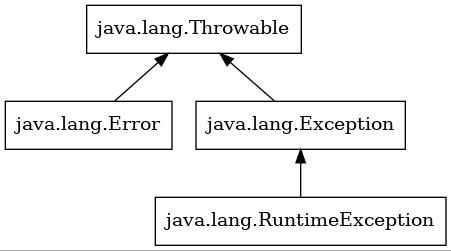
\includegraphics{exception}
\newline

The different kinds of exceptions are discussed in \autocite{ORACLE_DOC_LANGUAGE_SPECIFICATION:KindsOfExceptions}.

Exception classes that extend \lstinline|java.lang.Exception|\index{java.lang!Exception} are so-called \textit{checked} exceptions\index{exception!checked}\index{checked exception|see{exception}}; if a method wants to throw one of these, it has to declare that with the \lstinline|throws| clause. The class \lstinline|java.lang.RuntimeException|\index{java.lang!RuntimeException} is a direct subclass of \lstinline|java.lang.Exception|\index{java.lang!Exception} and the superclass of all \textit{runtime}\index{runtime exception|see{exception}} or \textit{unchecked}\index{exception!unchecked}\index{unchecked exception|see{exception}} exceptions – declaring these is not mandatory.

While an ordinary program can \textit{potentially} recover from an error condition signalled by an \lstinline|Exception|\index{java.lang!Exception} instance, it is assumed that instances of the class \lstinline|java.lang.Error|\index{java.lang!Error} and its subclasses will indicate unrecoverable error conditions, causing the program to abort.

The class of the thrown exception should be chosen appropriate to the error condition it indicates. So throwing just an instance  \lstinline|java.lang.Exception|\index{java.lang!Exception} or \lstinline|java.lang.RuntimeException|\index{java.lang!RuntimeException} is usually not a good idea – same if throwing a \lstinline|java.lang.NullPointerException|\autocite{ORACLE_DOC_NULLPOINTEREXCEPTION_CLASS}\index{java.lang!NullPointerException} in case a divisor is 0 (zero)\footnote{The proper exception class would be \lstinline|java.lang.ArithmeticException|\autocite{ORACLE_DOC_ARITHMETICEXCEPTION_CLASS}\index{java.lang!ArithmeticException}.}.

When selecting the exception class, your first look should be to the already existing exception implementations if there is already one that fits your needs.\footnote{Although sometimes the name of an exception looks good, you should also consider which package it lives in; throwing an exception from a JNDI related package like \lstinline|javax.naming.OperationNotSupportedException|\index{javax.naming!OperationNotSupportedException} in a code segment that does nothing with the “Java Naming and Directory Interface” at all will cause more confusion than it helps. Not to mention that it may require an additional module.} If none of the existing ones fit, implement your one exception class by extending one of \lstinline|Exception|\index{java.lang!Exception}, \lstinline|RuntimeException|\index{java.lang!RuntimeException}, or \lstinline|Error|\index{java.lang!Error}, depending on your needs\footnote{You can create your own exception class that extends \lstinline|Throwable|\index{java.lang!Throwable} directly, but so far I have not found a use case for that.}. This is always useful in the case of a feature library to simplify its API\footnote{All methods will only throw one exception especially created for that library, or exceptions derived from that. Samples for this pattern are the Servlet API (throwing only instances of \lstinline|IOException|\index{java.io!IOException} and \lstinline|ServletException|\index{javax.servlet!ServletException}) or JDBC (throwing only \lstinline|SQLException|\index{java.sql!SQLException} instances).}, and it can be also helpful for an application.

When implementing an extension or a server-based application (or when using a particular framework), you have to implement quite often methods that declare only one, sometimes two exceptions. Nevertheless, it may happen that a method call in your code throws an exception that cannot be handled by the current code, but it cannot be delegated also, because the interface for the method does not declare that particular exception. In such a case, you have to catch the exception and to wrap it into an instance of the declared exception that will be thrown afterwards. For a servlet implementation\autocite{JAKARTA_EE_HTTPSERVLET_CLASS}, this may look like this:
\begin{lstlisting}
protected final void doGet( HttpServletRequest request, HttpServletResponse response )
    throws ServletException, IOException
{
    …
    try
    {
        …
    }
    catch( final TimeOutException e )
    {
        throw new ServletException( e );
    }

    …
}  //  doGet()
\end{lstlisting}

When instantiating an exception instance, you should always provide a textual message that describes the error condition and/or provides additional information, like the name of the file that cannot be found, or the SQL statement with the invalid syntax.\footnote{In this regard, the sample above is bad, because it does not provide such an explanation.} These text have to be in English language, for the same reason why the names and the comments are in English.

Of course, messages that will be presented to the end user in a UI have to be localised, but the UI should not display the raw exception message anyway at all.

Some exception classes do not have a constructor that allows to provide a cause, or they have constructors that allow either a message or a cause, but not both. A sample for that is \lstinline|java.lang.ExceptionInInitializerError|\autocite{ORACLE_DOC_EXCEPTIONININITIALIZERERROR_CLASS}.

Some of these exception classes will allow a workaround that allows you to still provide both, cause and message, with them, like below:\footnote{Unfortunately, \lstinline|ExceptionInInitializerError| does not belong to this group of exception classes.}: 
\begin{lstlisting}
static
{
    try
    {
        …    
    }
    catch( final Exception e )
    {
        throw new DumpException( "Message" )
            .initCause( e );    
    }
}
\end{lstlisting}

For the method \lstinline|initCause()| refer to \autocite{ORACLE_DOC_THROWABLE:initCause}.

Unfortunately, you have to test whether the exception that you have to deal with allows this workaround. And you should add this test to the unit tests for your code, to protect you from changes coming with new versions.

%------------------------------------------------------------------------------

\subsection{General Exception Handling}\label{sec:GeneralExceptionHandling}
A method is only allowed to handle an exception if it is able to restore the program state, otherwise it has to delegate the exception. Delegation can be done either by ignoring the exception – in this case it will be propagated to the caller automatically (it “bubbles up”) – or by catching and wrapping it, as described in chapter \tqfullref{sec:ThrowingExceptions}.

To handle an exception you first have to catch it.

Catching \lstinline|java.lang.Exception| is discouraged in most cases; it \textit{can} be acceptable when you need to wrap all checked exceptions into a runtime exception or into an error:
\begin{lstlisting}
public final void run()
{
    try
    {
        …
    }
    catch( final Exception e )
    {
        throw new WrapperException( e );
    }
}   // run()
\end{lstlisting}

You should absolutely avoid to catch \lstinline|java.lang.Error| and all of its subclasses, \lstinline|java.lang.RuntimeException|, and of course, you should not never ever catch \lstinline|java.lang.Throwable|!\footnote{But no rule without an exception: refer to chapter \tqvref{sec:ExceptionHandlingInThreads}.}

Provide a \lstinline|catch| block for each and every exception that you want to handle:
\begin{lstlisting}
public final void run()
{
    try
    {
        …
    }
    catch( final FileNotFoundException e )
    {
        throw new ApplicationError( "Cannot find file", e );
    }
    catch( final IOException e )
    {
        throw new ApplicationError( "An error occurred on processing the input file", e );
    }
    catch( final NumberFormatException e )
    {
        throw new ApplicationError( "Input Data is corrupted", e );
    }
    catch( final PatternSyntaxException e )
    {
        throw new ApplicationError( "Pattern invalid", e );
    }
}   // run()
\end{lstlisting}

Sometimes when a large number of exceptions has to be handled with all the same code, you may be tempted to just catch \lstinline|java.lang.Exception|. As already said: don't do it! This approach will definitely cause problems as it may handle runtime exceptions in the same \lstinline|catch|-block as the checked exceptions, and usually this is not intended.

A simplificatin for the sample above could look like this:
\begin{lstlisting}
public final void run()
{
    try
    {
        …
    }
    catch( final IOException | NumberFormatException | PatternSyntaxException e )
    {
        throw new ApplicationError( "Processing failed", e );
    }
}   // run()
\end{lstlisting}
Still only the declared exceptions will be handled in the \lstinline|catch|-block, but unexpected exceptions will now bubble up\footnote{The exception class \lstinline|java.io.FileNotFoundException| is not listed because its superclass \lstinline|java.io.IOException| is already on the list.}.

Sometimes an exception indicates a regular program state (although this would indicate poor design in most cases)\footnote{Nevertheless, you can find this even in the Java Runtime Library~… but no one has ever said that the authors of the JDK had never made doubtful decisions.}. Usually you will avoid this situation by e.g. checking the operands before an operation, but a very popular example where this is not practicable is the conversion of a string into a numerical value:
\begin{lstlisting}
…
var amount = 0.0;
final var requestParam = request.getParameter( "amount" );
try
{
    if( nonNull( requestParam ) )
    {
        amount = Double.parseDouble( requestParam );
    }
}
catch( final NumberFormatException ignored )
{
    //---* If amount in request is not numeric, set it to 0.0 *------
    amount = 0.0;
}
…
\end{lstlisting}

As shown in the example, a comment is required in the catch clause, because you do not further propagate the exception neither do you log it.

It is also possible that you checked the preconditions, but you still have to deal with some checked exceptions:
\begin{lstlisting}
…
final var file = new File( … );
if( file.exists() )
{
    try( final var input = new FileInputStream( file ) )
    {
        …
    }
    catch( final FileNotFoundException e )
    {
        throw new UnexpectedExceptionError( "File was there when checked!", e );
    }
}
…
\end{lstlisting}

A sample for the class \lstinline|UnexpectedExceptionError| can be found in \autocite{TQUADRAT_ORG_FOUNDATION_UNEXPECTEDEXCEPTIONERROR}.

Some APIs in the JDK declares a checked exception, but that will never be thrown for the given arguments by any means. Most famous for this are the conversions from byte arrays to Strings and back:
\begin{lstlisting}
…
final String s;
try
{
    s = new String( byteArray, "UTF-8" );
}
catch( final UnsupportedEncodingException e )
{
    throw new ImpossibleExceptionError( "UTF-8 must exist!", e );
}
…
\end{lstlisting}

According to \autocite{ORACLE_DOC_CHARSET:StandardCharsets}, the UTF-8 encoding is mandatory for each JDK/JVM implementation, therefore the code sequence above will \textit{never} throw an \lstinline|UnsupportedEncodingException|. Nevertheless, it is not allowed to swallow the exception; instead an error should be thrown in the \lstinline|catch| clause, indicating the error condition. In the improbable case UTF-8 is not supported by the current Java runtime environment, the problem will surface, and the program will not die silently without any hint about the reason.\footnote{If, of course, there is no catch for \lstinline|Throwable| somewhere on the path.} It also protects you from malicious changes to the name of the character encoding: a none existing \lstinline|Charset| will cause noise.

Of course, the problem could be solved differently, by using an instance of \lstinline|java.nio.charset.Charset|\autocite{ORACLE_DOC_CHARSET_CLASS} as the argument to the \lstinline|String| constructor, instead of the name of the character encoding. For this case, the constructor does not declare an \lstinline|UnsupportedEncodingException|. 

Another example is the interface \lstinline|java.lang.Appendable|\autocite{ORACLE_DOC_APPENDABLE_INTERFACE}: it is implemented by \lstinline|java.io.Writer| and \lstinline|java.io.PrintStream|, but also by \lstinline|java.lang.StringBuilder| (and a few more). The method \lstinline|java.lang.Appendable::append| declares to throw an \lstinline|IOException|, but the implementation of that method for \lstinline|StringBuilder| will never throw it and does not even declare it.
\begin{lstlisting}
…
final Appendable appendable = new StringBuilder();
try
{
    appendable.append( "Some Text" );
}
catch( final IOException e )
{
    throw new ImpossibleExceptionError( "Append to StringBuilder", e );
}
…
\end{lstlisting}

Again, a sample for \lstinline|ImpossibleExceptionError| can be found in \autocite{TQUADRAT_ORG_FOUNDATION_IMPOSSIBLEEXCEPTIONERROR}.

Sometimes a method wants to act upon an error condition without handling the exception. In this case, it may catch the exception, does whatever necessary, then throw it again. An example:
\begin{lstlisting}
public final void myMethod() throw IOException
{
    final Predicate<String> isNetworkError = m_NetworkErrorPattern.asMatchPredicate();
    …
    try
    {
        …
    }
    catch( final IOException e )
    {
        final var message = e.getMessage();
        if( nonNull( message ) && isNetworkError.test( message ) ) ++networkErrors;
        throw e;
    }
    …
}   // myMethod()
\end{lstlisting}

It is usually not a good idea to log an exception and to rethrow or to wrap it afterwards, because this might cause the exception to be logged twice (or even more often). More details about logging can be found in chapter \tqvref{sec:Logging}.

Finally, you handle the exception somehow, by assigning a default value\footnote{see the sample about the conversion from string to number, above.}, or by performing an alternative action. In any case, you need to provide a comment in the \lstinline|catch| why you do not further delegate the handling of the exception.

If an exception was not caught in your code, it ”bubbles up” until it reaches the main method for the current thread (that is \lstinline|main()| for the main or program thread, and \lstinline|run()|\autocite{ORACLE_DOC_RUNNABLE:run} for any other thread). If this method will not handle the exception, the thread will be aborted. If this thread is the last non-deamon thread, the JVM will be terminated, too.

%------------------------------------------------------------------------------

\subsection{Exceptions in Threads}\label{sec:ExceptionHandlingInThreads}
When we execute the Java program below, the \lstinline|Error| is printed to the console:
\lstinputlisting[numbers=left,caption={Test Abort main()}]{TestAbortMain.java}

\begin{verbatim}
$ java TestAbortMain.java
Exception in thread "main" java.lang.Error: Aborted
    at TestAbortMain.main(TestAbortMain.java:5)
$ 
\end{verbatim}

In the sample below, we abort a secondary thread:
\lstinputlisting[numbers=left,caption={Test Abort run()}]{TestAbortRun.java}

The output looks like this\footnote{When using an older version of Java, no output from the thread would be shown at all.}
\begin{verbatim}
$ java TestAbortRun.java
Exception in thread "Thread-0" java.lang.Error: run() aborted!
    at TestAbortRun.run(TestAbortRun.java:5)
    at java.base/java.lang.Thread.run(Thread.java:833)
Exception in thread "main" java.lang.Error: main() aborted!
    at TestAbortRun.main(TestAbortRun.java:20)
$ 
\end{verbatim}

This behaviour is sufficient for a tool in most cases, but not for a standalone application and not for a feature library. A function library usually relies on the a caller, while serverbase applications and extensions use the facilities provided by the host applications.

For both a standalone application and for a feature library, you want that error conditions will be logged, under all circumstances.

For the main thread of an application this can be achieved quite easily, by implementing the method \lstinline|main()| like this:
\begin{lstlisting}
/**
 *  The program entry method.
 *
 *  @param  args    The command line arguments.
 */
public static final void main( final String... args )
{
    try
    {
        final var application = new MyClass();
        applicaton.execute( … );
    }
    catch( final Throwable t )
    {
        //---* Log the previously unhandled exceptions *-------------
        m_Logger.error( "Unhandled Exception/Error", e );
    }
}   //  main()
\end{lstlisting}
In this case, the \lstinline|catch| statement catches \lstinline|Throwable| and the 
\lstinline|catch|-block does nothing else but logging the exception!

This is acceptable here only because the program ends immediately after the closing curly brace of the \lstinline|catch|-block!\footnote{Ok, technically only the main thread ends here because other non-deamon threads may still run at this point. But the goal should be that the main thread dies always at last.}

Theoretically, you can do the same thing for threads:
\begin{lstlisting}
public final void run()
{
    try
    {
        //---* The thread's payload *--------------------------------
        …
    }
    // NOT Recommended
    catch( final Throwable t )
    {
        //---* Log the previously unhandled exceptions *-------------
        m_Logger.error( "Unhandled Exception/Error", e );
    }
}   //  run()
\end{lstlisting}

One reason is that the method \lstinline|Runnable::run|\autocite{ORACLE_DOC_RUNNABLE:run} can be called also in other contexts than just as the main method of a thread; swallowing the exception like shown in the example is a bad idea in that case.

Another reason is that when the method is implemented as part of a library, an extension or even a server-based application, different facilities may be used to report the error.

But the main reason is that there is a much better mechanism that handles those otherwise unhandled exceptions: the “Uncaught Exception Handler”\autocite{ORACLE_DOC_UNCAUGHTEXCEPTIONHANDLER_INTERFACE}.

The interface \lstinline|java.lang.Thread.UncaughtExceptionHandler| is a functional interface\autocite{ORACLE_DOC_LANGUAGE_SPECIFICATION:FunctionalInterfaces, ORACLE_DOC_LANGUAGE_SPECIFICATION:FunctionalInterface, ORACLE_DOC_FUNCTIONALINTERFACE_ANNOTATION} providing the method \lstinline|uncaughtException()|\autocite{ORACLE_DOC_UNCAUGHTEXCEPTIONHANDLER:uncaughtException}.

There are basically two ways\footnote{In fact, three ways. But as you should avoid anonymous classes, this option is omitted here.} to implement an uncaught exception handler; the classical way would be to create a new class:
\begin{lstlisting}[numbers=left,caption={Class UncaughtExceptionHandlerImpl}]
/**
 *  The implementation of the interface
 *  {@link java.lang.Thread.UncaughtExceptionHandler}
 *  that is used by this project.
 */
public final class UncaughtExceptionHandlerImpl implements Thread.UncaughtExceptionHandler
{
    /**
     *  The logger that is used to report the uncaught exceptions.
     */
    private static final Logger m_Logger = getLogger( UncaughtExceptionHandlerImpl.class );
     
    /**
     *  {@inheritDoc}
     */
    @Override
    public final void uncaughtException( final Thread t, final Throwable e )
    {
        m_Logger.error( "Unhandled Exception/Error in Thread '%s'".formatted( t.getName(), e );
    }   //  uncaughtException()
}
//  class UncaughtExceptionHandlerImpl 
\end{lstlisting}

Otherwise you can benefit from \lstinline|java.lang.Thread.UncaughtExceptionHandler| being a functional interface and implement the uncaught exception handler as a method in your class:
\begin{lstlisting}
public final class MyClass
{
    /**
     *  The logger that is used by this class.
     */
    private static final Logger m_Logger = getLogger( MyClass.class );
     
    /**
     *  <p>{@summary This method will be invoked when the given
     *  thread terminates due to the given uncaught exception.}</p>
     *  <p>Any exception thrown by this method will be ignored by
     *  the Java Virtual Machine.</p>
     *
     *  @param  t   The thread that terminated.
     *  @param  e   The exception that caused the termination.
     *     
     *  @see UncaughtExceptionHandler#uncaughtException(Thread,Throwable)
     */
    private final void uncaughtException( final Thread t, final Throwable e )
    {
        m_Logger.error( "Unhandled Exception/Error in Thread '%s'".formatted( t.getName(), e );
    }   //  uncaughtException()
}
//  class MyClass
\end{lstlisting}
In the second case, the uncaught exception handler uses the resources provided by the class it lives in. This may be desired or not.

A thread can be configured with the uncaught exception handler in three different ways:
\begin{enumerate}
\item{Each single thread can get its own uncaught exception handler by calling \lstinline|setUncaughtExceptionHandler()|\autocite{ORACLE_DOC_THREAD:setUncaughtExceptionHandler} on it, with an instance of an implementation of \lstinline|Thread.UncaughtExceptionHandler| as the argument:
\begin{lstlisting}
public final class MyClass
{
    /**
     *  Does the program's work.
     *
     *  @throws InterruptedException   The worker thread was
     *      interrupted.
     */
    private final void execute() throws InterruptedException
    {
        final var thread = new Thread( this::run, "MyWorkerThread" );
        thread.setUncaughtExceptionHandler( this::uncaughtException );
        thread.start();
        thread.join();
    }   //  execute()
     
    /**
     *  The thread's main method.
     */
    private final void run() { … }
}
//  class MyClass
\end{lstlisting}
}

\item{On creation of a thread, a \lstinline|ThreadGroup|\autocite{ORACLE_DOC_THREADGROUP_CLASS} instance will be assigned to it; if none is explicitly set, it will be the group of the current thread.

The instance has a method \lstinline|uncaughtException()|\autocite{ORACLE_DOC_THREADGROUP:uncaughtException} method is called in the case the thread itself does not have an uncaught exception handler assigned to it. To change the behaviour of the handler from the thread group it is necessary to derive a new class from \lstinline|ThreadGroup| and to overwrite the \lstinline|uncaughtException()|.

Chapter \tqvref{sec:ThreadGroup} shows an implementation for \lstinline|ThreadGroup| (named \lstinline|ThreadGroupExt|) that allows to configure the uncaught exception handler; when using that class, the configuration can look like this:
\begin{lstlisting}
public final class MyClass
{
    /**
     *  The thread group for all threads used by this program.
     */
    private final ThreadGroup m_ThreadGroup;
    
    /**
     *  Creates a new instance of {@code MyClass}.
     */
    public MyClass()
    {
        m_ThreadGroup = new ThreadGroupExt( "MyWorkerThreads", this::uncaughtException );
    }   //  MyClass()
    
    /**
     *  Does the program's work.
     *
     *  @throws InterruptedException   The worker thread was
     *      interrupted.
     */
    private final void execute() throws InterruptedException
    {
        final var thread = new Thread( m_ThreadGroup, this::run, "MyWorkerThread" );
        thread.start();
        thread.join();
    }   //  execute()
     
    /**
     *  The thread's main method.
     */
    private final void run() { … }
}
//  class MyClass
\end{lstlisting}
}
\item{By calling \lstinline|java.lang.Thread::setDefaultUncaughtExceptionHandler|\autocite{ORACLE_DOC_THREAD:setDefaultUncaughtExceptionHandler} it is possible to install an instance of \lstinline|Thread.UncaughtExceptionHandler| for all threads that does neither have their own handler nor got one from their thread group. This uncaught exception will be called as a last resort.
\begin{lstlisting}
public final class MyClass
{
    /**
     *  Does the program's work.
     *
     *  @throws InterruptedException   The worker thread was
     *      interrupted.
     */
    private final void execute() throws InterruptedException
    {
        //---* Install the default uncaught exception handler *------
        Thread.setDefaultUncaughtExceptionHandler( new UncaughtExceptionHandlerImpl() );
        
        final var thread = new Thread( this::run, "MyWorkerThread" );
        thread.start();
        thread.join();
    }   //  execute()
     
    /**
     *  The thread's main method.
     */
    private final void run() { … }
}
//  class MyClass
\end{lstlisting}
}
\end{enumerate}

The last option can be used only from standalone applications and from tools. The environments for server-based applications and extensions do quite often restrict the creation of additional threads. A feature library should accept an uncaught exception handler and/or a thread group as a configuration value.

If a function library creates new threads, the respective methods must accept at least an uncaught exception handler and optionally a thread group. Alternatively, a thread factory\autocite{ORACLE_DOC_THREADFACTORY_INTERFACE} can be injected.
 
%------------------------------------------------------------------------------

\subsection{Reporting Errors}\label{sec:ReportingErrors}
As already said earlier, at some point we need to report an error condition to the user of our program; this can happen in various ways. The most common is to log the error somehow, but as logging has various additional aspects, it is covered by a chapter of its own: chapter \tqfullvref{sec:Logging}.

Other means to report the error condition are the following:
\begin{itemize}
\item{Write an error message to the console, a message window or status bar.}
\item{Display an error dialog.}
\item{Send an email, a tweet or another kind of message.}
\item{Trigger an external signalling device (an alarm bell, a horn, a flashlight,~…).}
\item{…}
\end{itemize}

Before discussing this further, I want to repeat: \textit{Reporting an error condition is not handling it!}

Obviously, not all ways of reporting an error condition are feasible for all types of products.

\begin{itemize}
\item{First, a \textit{function library} should not report an error condition in any other way than just throwing the appropriate exception. It should not even log them.}

\item{\textit{Extensions} and \textit{server-based applications} should use the APIs that are provided to them by their hosts/containers for reporting the error conditions, although server-based applications may introduce additionals ways to report an error.}

\item{Code in a \textit{function library}, in a \textit{server-based application} and in an \textit{extension} should never write to the console or display an error dialog. The code of a \textit{feature library} can use a message window, status bar or error dialog, if it provides these resources itself (basically, when it provides the UI).

Application servers, frameworks and the hosts for extensions usually provides a facility for error reporting that can be used; this may result in updating a message window or status bar, but for your code, this is transparent.}

\item{Sending messages around to report an error condition should be considered mainly for dark (headless) applications, either standalone or server-based. Of course, this something that can be provided by a feature library (as the new featured), but a feature library should not use it.

Whether it makes sense for a tool depends on the kind of the tool.}

\item{Same for the use of external signalling devices.}
\end{itemize}

In most cases, it is not sufficient to provide the user with the caught exception only – meaning just calling \lstinline|java.lang.Throwable::printStackTrace| is not enough. In fact, for most users, this is even too much information. Also providing the call stack for an operation in an \textit{error message} is sometimes considered as a security loophole, because it may give a potential attacker information about code internals that they can use to shape their attack against your system.

You should also consider to localise the error message to the locale of the user; that is mainly translating it to the user's language, but not only. You should always add the time zone to timestamps, or at least the offset to UTC, even when you adjust them to the user's time zone.

It is a good idea to have a unique error code with your error message. That allows you to identify it when the user reports it back to you, and you do not understand their language. 

Obviously, you should avoid to have sensitive data in your error messages. But ‘sensitive data’ may depend from the context your program is running in.

%------------------------------------------------------------------------------

\subsection{Logging}\label{sec:Logging}
Logging is a mean to report errors and to make the respective messages available even after the program is down, for a post~mortem analysis. But you can use logging for other purposes, too.

Nevertheless, \textit{logging} is mainly for the recording of technical issues. If you need to keep track of business transactions (if you have to provide an audit log or a journal), we talk about \textit{journalling} instead. There may be some overlapping between those two, and the requirements look similar, but logging and journalling are two distinct topics and should be treated independently from each other.

Another only slightly related topic is performance logging or monitoring where you issue alert messages in case operations took longer than expected. Of course these can be written to the regular error logs, but in most cases, you should consider a dedicated infrastructure for this feature.

%------------------------------------------------------------------------------

\subsubsection{Logging Infrastructure}
The simplest way to implement logging would be to open a file during startup and to write the log messages there. That works, but this is not very flexible, although it might be sufficient for a tool.

Because logging is an important feature, Java comes with a logging facility right out of the box, the so called ‘JDK~Logging’\footnote{Sometimes also referred to as ‘JUL’, by the name of the package.}, provided by the package \lstinline|java.util.logging|\autocite{ORACLE_DOC_LOGGING_PACKAGE, ORACLE_DOC_LOGGING_OVERVIEW}.

Despite the fact that it has improved significantly since its introduction with Java~1.4, most people prefer still use the logging subsystem provided by the external Log4j\autocite{APACHE_LOG4J} library.

Next, only tools and standalone applications should configure a logging framework. Function libraries should not log at all, while feature libraries rely on the logging facilities provided by the host environment, same as server-based applications and extensions.

For the latter two the host environment also defines the whole API for logging, but for feature libraries (and for function libraries that really require logging) it is recommended to integrate the SLF4J\autocite{SLF4J} library.

SLF4J is not a logging framework itself, the library provides only a facade for a logging framework (“SLF4J” stands for “Simple Logging Facade for Java”), its methods delegate to a \textit{real} logging framework; refer to \autocite{SLF4J:Binding} on how this is done. Originally, the API was inspired from Log4j, but it has evolved since then. SLF4J supports Log4j, JDK~Logging, Apache Commons Logging\autocite{APACHE_COMMONS_LOGGING} (formerly known as JCL – Jakarta Commons Logging) and Logback\autocite{LOGBACK} as well as ‘Simple’ logging. Support for other frameworks can be implemented easily if required.

Looking at the code to write, all three (JDK~Logging, Log4j and SLF4J) work basically the same:
\begin{enumerate}[nosep]
\item{During the initialisation of your class, obtain an instance of a logger class; the instances are named, usually by the name of the the class that obtains it\footnote{This is discussed in more detail in chapter \tqvref{sec:NamingOfLoggers}.}. These names are used for the configuration of a logger.}

\item{Keep the reference in a \lstinline|private static final| variable with the name \lstinline|m_Logger|.}

\item{Check whether the desired log level is active.}

\item{If the desired log level is active, log your message.}
\end{enumerate}

Even the APIs are quite similar, down to the names\footnote{Of course the code sample will not compile.}: 
\begin{lstlisting}[numbers=left]
// For JDK Logging:
import static java.util.logging.Logger.getLogger;
import static java.util.logging.Level.*; 
import java.util.logging.Logger;

// For Log4j:
import static org.apache.logging.log4j.LogManager.getLogger;
import static org.apache.logging.log4j.Level.*;
import org.apache.logging.log4j.Logger;
import org.apache.logging.log4j.message.*;

// For SLF4J:
import static org.slf4j.LoggerFactory.getLogger;
import org.slf4j.Logger;

public final class MyClass
{
       /*------------------------*\
    ===** Static Initialisations **==================================
       \*------------------------*/
    /**
     *  The logger that is used by this class.
     */
    private static final Logger m_Logger = getLogger( MyClass.class.getName() );
    
    /* For Log4j and SLF4J, this works, too: */
    private static final Logger m_Logger = getLogger( MyClass.class );
    
    /* For Log4j, even this will have the same result: */
    private static final Logger m_Logger = getLogger();
    
       /*---------*\
    ===** Methods **=================================================
       \*---------*/
    public final void myMethod()
    {
        //---* Logging an error message *----------------------------
        final var message = "An error occurred!";
        final var error = new Error( "Something happened!" );
        
        /* With JDK Logging */
        m_Logger.severe( message ); // Without the exception …
        m_Logger.log( SEVERE, message, error );
        
        /* With Log4j and SLF4J */
        m_Logger.error( message, error );
        
        /* With Log4j */
        m_Logger.log( ERROR, message, error );
        m_Logger.atError()
            .withThrowable( error )
            .log( message );

        //---* Logging an informational message *--------------------
        /* With JDK Logging */
        if( m_Logger.isLoggable( INFO ) )
        {
            final var message = getCurrentStatus();
            m_Logger.log( INFO, message );
        }
        
        /* With Log4j and SLF4J */
        if( m_Logger.isInfoEnabled() )
        {
            final var message = getCurrentStatus();
            m_Logger.info( message );
        }
        
        /* With Log4j */
        m_Logger.atInfo()
            .log( () -> new SimpleMessage( getCurrentStatus ) );
    }   //  myMethod()
}
//  class MyClass
\end{lstlisting}

For the details, refer to the respective documentation:
\begin{itemize}[nosep]
\item{JDK~Logging: \lstinline|java.util.logging.Logger|\autocite{ORACLE_DOC_LOGGER_CLASS}}
\item{Log4j: \lstinline|org.apache.logging.log4j.Logger|\autocite{APACHE_LOG4J:Logger}}
\item{SLF4J: \lstinline|org.slf4j.Logger|\autocite{SLF4J:Logger}}
\end{itemize}

%------------------------------------------------------------------------------

\subsubsection{The Log Levels}\label{sec:LogLevels}
A logger can be configured that it logs only messages with at least a certain priority or \textit{log level}. For JDK~Logging, Log4j and SLF4J, the predefined log levels differ:
\begin{filecontents}{LogLevels.tbl}
  \begin{longtable}{|c|c|c|X|}
  \caption{Log Levels} \\
  \hline 
  JDK~Logging & Log4j & SLF4J & Description \\ 
  \hline
  \endfirsthead
  \multicolumn{4}{c}%
  {\tablename\ \thetable\ -- \textit{Continued from previous page}} \\
  \hline 
  JDK~Logging & Log4j & SLF4J & Description \\ 
  \hline
  \endhead
  \multicolumn{4}{r}{\textit{Continued on next page}} \\ 
  \endfoot
  \endlastfoot
  & \verb#FATAL# & & A fatal event that will prevent the application from continuing. \\
  \hline
  \verb#SEVERE# & \verb#ERROR# & \verb#ERROR# & An error in the application, possibly recoverable. A message level indicating a serious failure. \\ 
  \hline 
  \verb#WARNING# & \verb#WARN# & \verb#WARN# & An event that might possibly lead to an error. \\ 
  \hline 
  \verb#INFO# & \verb#INFO# & \verb#INFO# & An event for informational purposes. \\ 
  \hline 
  \verb#CONFIG# & & & A message level for static configuration messages. \\ 
  \hline 
  \verb#FINE# & \verb#DEBUG# & & A general debugging event. A message level providing tracing information. \\ 
  \hline 
  \verb#FINER# & & & A fairly detailed tracing message.\\
  \hline 
  \verb#FINEST# & \verb#TRACE# & \verb#TRACE# & A fine-grained debug message, typically capturing the flow through the application. A highly detailed tracing message. \\
  \hline 
 \end{longtable} 
\end{filecontents}
\LTXtable{\linewidth}{LogLevels.tbl}
In addition, they also know the ‘levels’ \verb#ALL# (log everything) and \verb#OFF# (log nothing), but you cannot check for these.

A lower level includes all the higher levels, too. So when a logger is configured for the log level \verb#INFO#, \lstinline|m_Logger.isLoggable()| will return \lstinline|true| for \verb#INFO#, \verb#WARNING# (or \verb#WARN#), \verb#SEVERE#, \verb#ERROR# and \verb#FATAL#, but not for \verb#DEBUG# or \verb#FINER#.

JDK~Logging and Log4j allow both to define additional log levels. Basically, this is also possible for SLF4J, but without knowlegde about the implementation that is really used for logging, it is quite difficult to determine how these new log levels in SLF4J are mapped to those of the effective logging framework.

So sometimes you want to have a log level that allows to log informational messages under all circumstances. Of course you could use \verb#SEVERE# or \verb#FATAL# for that purpose, but that would pollute the logs with false error messages. A better idea would be to introduce a log level \verb#INFO_FORCED# or \verb#VITAL#.

The example below shows how to create additional log levels for the JDK~Logging:
\lstinputlisting[numbers=left,caption={LogLevel.java for JDK~Logging}]{LogLevel.java}

To create a log level \verb#INFO_FORCED# for Log4j, create the respective constant somewhere in your code:
\begin{lstlisting}
public final ApplicationMainClass
{
    …
    
        /*------------------------*\
    ====** Static Initialisations **=================================
        \*------------------------*/
    /**
     *  The log level &quot;{@code INFO_FORCED}&quot;.
     */
    public static final Level INFO_FORCED = Level.forName( "INFO_FORCED", 1 );
    
    …
}
//  class ApplicationMainClass
\end{lstlisting}

\textbf{Note:} For Log4j, the integer value for the higher log level is closer to \lstinline|0| (zero), while for JDK~Logging, it is closer to \lstinline|Integer.MAX_VALUE|.

With Log4j, you can achieve a similar result by using \lstinline|Logger::always|\autocite{APACHE_LOG4J:Logger.always}\index{org.apache.logging.log4j!Logger!always()} instead of creating a new log level:
\index{org.apache.logging.log4j!Logger!always()}\index{org.apache.logging.log4j!Logger!withThrowable()}\index{org.apache.logging.log4j!Logger!withLocation()}\index{org.apache.logging.log4j!Logger!log()}
\begin{lstlisting}
…
m_Logger.always()
    .withThrowable( e )
    .withLocation()
    .log( "Vital message!" );
…    
\end{lstlisting}

%------------------------------------------------------------------------------

\subsubsection{How to log}\label{sec:HowToLog}
This chapter discusses how to emit log messages, but also when you should log something, and what you should log.

\paragraph{Errors} First, you should log error conditions at some point in the program flow. Usually this means that you will log an exception. And you will log an exception only when you do not further delegate the handling of that exception. For tools and standalone applications, this means that you will log an exception latest in the \lstinline|main()| method or in the \lstinline|UncaughtExceptionHandler| for threads other than the main thread (refer to chapter \tqfullvref{sec:ExceptionHandlingInThreads}).

We said already that a function library will not log at all. For a feature library, an extension and server-based application, you should log when the control flow is about to leave the realm of your component and you do not know how the host code will handle the exception (or if it will handle and/or them at all).

You should also log (uncaught) exceptions in threads that your code creates; this was already discussed in chapter \tqfullref{sec:ExceptionHandlingInThreads}.

As a rule of thumb, you log an exception at the latest possible occasion.

The log message should contain all information that you have a this point; this is at least the exception itself with its message and stacktrace. But perhaps you know additional things, for example what your code attempted when the exception was thrown, that name of resources that should be tried to access, the user name, the access rights and many other things – as long as these are not sensible data! So you should never add a password to a log message. And even the user name is already in a gray area.

Obviously, the log levels \verb#FATAL#, \verb#SEVERE# and \verb#ERROR# are meant for these messages. The other log levels are not meant for reporting \textit{current} error conditions.

\paragraph{Warnings} The description for the log levels \verb#WARNING# and \verb#WARN# says that these indicate “an event that might possibly lead to an error” somewhen in the future.

Such an event could be the repeatingly failed login attempt of a user, as that could be the indication for a hacker attack. Most probably, you should not log the first failed attempt, perhaps not even the second or third (at least not as a warning), but consecutive attempts from the same device and/or with the same user name should be logged. And obviously, the respective log message must contain all the necessary data that can be used to repel that attack. Whether the used passwords should be added to the log messages can be discussed.

Obviously, you have to implement the necessary infrastructure to collect the data for all failed (and successful) logins, and you do this only to be able to log the respective warning.\footnote{Although you can collect this data also for general monitoring if your application lives in an environment where this is provided. Or you make it available through JMX – see chapter \tqvref{sec:UtilisingJMX}.} This means that you can switch it off when the log level is disabled.

In the same way, you should log attempts of unauthorised access to data or functionality by authenticated users.

Another reason to log a warning would be when you handle an error condition by repeating an operation or by performing an alternative operation. Although the current problem is solved for now, it is worth to keep track of it in the logs.

Then you should emit a warning to the logs when a resource gets short, but before it is exhausted; even when the application recovers from that, it should be tracked. If you run out of a particular resource, this would be an error condition, no longer a warning condition.

Obviously, this is not a complete list.

\paragraph{Info} You \textit{may} also log other important events that are clearly no error condition nor a warning. The log level for this kind of log entries is \verb#INFO#. You should assume that this is the default log level for each new logger, meaning that messages with the log levels \verb#INFO#, \verb#WARNING#/\verb#WARN# and \verb#FATAL#/\verb#ERROR#/\verb#SEVERE# are always written to the log file.

An \verb#INFO# log message may be confirmation for the successfully established connection with an external system, for the start and the termination of a long running background process, for the creation of a new user and alike.

It is also a good idea to log the system configuration on startup with the log level \verb#INFO#. The log level \verb#CONFIG# from JDK~logging is lower than \verb#INFO#, therefore using that may cause unwanted behaviour. 

You should not log (at least not with a log level of \verb#INFO#) the successful termination of common operations.\footnote{The kind of application that you create may request an audit log of some kind, but this is not covered by \textit{logging}. Instead we talk about \textit{journalling} here.}

In general, you should avoid to log the “happy path” in your code – at least, you should not do this with the log level \verb#INFO#.

\paragraph{Debug and Trace} A very basic technic for the debugging of a program is to add statements to the code that prints the current state to the console.

Logging with the log levels \verb#DEBUG#, \verb#TRACE#, \verb#FINE#, \verb#FINER#, and \verb#FINEST# is basically the same, just with the difference that you do not emit to a console, but to the log file.

There are some recommendations to log the entry and exit for each method, together with the arguments and the return value. In JDK~Logging, the class \lstinline|java.util.logging.Logger| has a set of specialised methods to support this approach (\lstinline|Logger::entering| and \lstinline|Logger::exiting|) that emit messages with the log level \verb#FINER#. That will look like this:
\begin{lstlisting}
public final class myClass
{
    private static final String CLASS_NAME = myClass.class.getName();
    private static final Logger m_Logger = getLogger( CLASS_NAME );
    
	…    
    
    public final String myMethod( final String value, final boolean flag )
    {
        final var METHOD_NAME = "myMethod";
        m_Logger.entering( CLASS_NAME, METHOD_NAME, value, Boolean.valueOf( flag ) );
        
        //---* Does some work here … *-------------------------------
        …
    
        //---* Done *------------------------------------------------
        m_Logger.exiting( CLASS_NAME, METHOD_NAME, retValue );
        return retValue;
    }   //  myMethod()
}
//  class myClass
\end{lstlisting}

Log4j has the methods \lstinline|Logger::traceEntry| and \lstinline|Logger::traceExit| for the same purpose, that are easier to use:
\begin{lstlisting}
public final class myClass
{
    private static final Logger m_Logger = getLogger();
    
	…    
    
    public final String myMethod( final String value, final boolean flag )
    {
        m_Logger.traceEntry( "value: %s - flag: %b", value, Boolean.valueOf( flag ) );
        
        //---* Does some work here … *-------------------------------
        …
    
        //---* Done *------------------------------------------------
        m_Logger.traceExit( retValue );
        return retValue;
    }   //  myMethod()
}
//  class myClass
\end{lstlisting}

But you should be careful with applying these methods to your code. First, because the kind of information provided by this kind of logging is useful only in rare case. And next, if really each and every method is instrumented in that way, the log files will be flooded with messages when the general log level is set to \verb#FINER# or \verb#FINEST# for JDK~Logging or \verb#TRACE# for Log4j respectively, making it very difficult to find the information you really need.

In addition, for JDK~Logging, it requires a real lot amount of unnecessary code to write, because neither the name of the class nor that of the method will be detected automatically; instead, these values have to be provided as a constant. That also makes some refactorings quite challenging~…

As a result, I do not recommend to use entry/exit logging. In fact, you should generally think twice before you add a log statement for \verb#DEBUG# and \verb#TRACE# proactively.

Of course, there are scenarios that are well known to cause issues during runtime quite often and therefore \verb#DEBUG# logging should be added for them. One good sample is the processing of emails, others are REST and SOAP communications.

But in general, you should never add \verb#TRACE# logging \textit{proactively}, and \verb#DEBUG# logging only in special cases.

On the other hand, you should never remove \verb#DEBUG# and \verb#TRACE# logging that you added during a bug hunt; it may get useful again if a regression tests fails. This also means that the \verb#DEBUG# and \verb#TRACE# log messages should be very verbose so that you can identify them even years later.
\begin{lstlisting}
public final String myMethod( final String value, final boolean flag )
{
    // DISCOURAGED!!
    m_Logger.trace( value );
    
    // RECOMMENDED
    m_Logger.trace( "BUGHUNT_2022-12-14 - entering myMethod()|value = '{}', flag = {}", value, flag );
    
    final var buffer = retrieveData( value, flag );
    
    // DISCOURAGED
    m_Logger.debug( buffer );
    
    // RECOMMENDED
    if( m_Logger.isDebugEnabled )
    {
        m_Logger.debug( "BUGHUNT_2022-12-14 - myMethod() called retrieveData()|value = '{}', flag = {}", value, flag );
        if( isNull( buffer )
        {
            m_Logger.debug( "BUGHUNT_2022-12-14 - retrieveData() returned null!" );
        }
        else
        {
            m_Logger.debug( "BUGHUNT_2022-12-14 - retrieveData() returned '{}'", buffer );
        }
    }
    
    final var retValue = process( buffer );
    
    //---* Done *----------------------------------------------------
    // DISCOURAGED
    m_Logger.debug( retValue );
    
    // RECOMMENDED
    m_Logger.trace( "BUGHUNT_2022-12-14 - exting myMethod()|retValue = '{}'", retValue );
    
    return retValue;
}   //  myMethod()
\end{lstlisting}

In chapter \tqref{sec:GeneralExceptionHandling} I said that it is usually not a good idea to log an exception and to rethrow or to wrap it afterwards. But there is one exception to this rule: sometimes you want to know about an exception that will be handled later and will be not logged then. Or you have some additional information at the current code location that you cannot add to the wrapper exception (perhaps because of its size). In this case, you can log that exception for debugging (the sample uses Log4j/SLF4J): 
\begin{lstlisting}
public final void myMethod() throw IOException
{
    …
    try
    {
        …
    }
    catch( final IOException e )
    {
        //---* Log and rethrow *-------------------------------------
        m_Logger.catching( DEBUG, e );
        throw e;
    }
    …
    try
    {
        …
    }
    catch( final IllegalStateException e )
    {
        //---* Log and wrap *----------------------------------------
        if( m_Logger.isDebugEnabled() )
        {
            final var message = composeIllegalStateContextMessage();
            m_Logger.debug( message, e );
        }    
        throw new ApplicationError( "Already in use", e );
    }
    …
}   // myMethod()
\end{lstlisting}

Here you also accept that the same exception might be logged twice.

\paragraph{Configuration} I have to confess that I never understood the purpose of the log level \verb#CONFIG# for the JDK~Logging. The description says “A message level for static configuration messages”. So you should use it to log the configuration parameters of your program – things like the current IP address, but also the system properties, or at least the command line parameters.

Of course, these could be relevant information for debugging issues, and it would make sense to log them with each restart of your program.

But \verb#CONFIG# has a lower priority than \verb#INFO# – this means that when you activate \verb#CONFIG#, you have also activated \verb#INFO# for that logger. This is probably not wanted.

Therefore most people uses a dedicated logger\footnote{refer to chapter \tqfullvref{sec:NamingOfLoggers}.} to log the configuration settings – but this makes the log level \verb#CONFIG# completely obsolete.

My recommendation would be to completely ignore the log level \verb#CONFIG# and to use a dedicated logger with log level \verb#INFO# instead. If you are using another logging framework than JDK~Logging, you don't have another choice either.

%------------------------------------------------------------------------------

\subsubsection{Naming of Loggers}\label{sec:NamingOfLoggers}
Each call to \lstinline|Logger::getLogger| (for JDK~Logging), \lstinline|LogManager::getLogger| (for Log4j), or \lstinline|LoggerFactory::getLogger| (for SLF4J) with the same argument will always return the \textit{same} logger instance:
\begin{lstlisting}
if( MyClass.class
    .getName().equals( "org.tquadrat.foundation.sample.logging.MyClass" ) )
{
    // Always true!!
    getLogger( MyClass.class.getName() )
        == getLogger( "org.tquadrat.foundation.sample.logging.MyClass" );
}
\end{lstlisting}

This means that a logger is created just once for a given name.

Both JDK~Logging and Log4j organise their loggers in a parent-child hierarchy with a root logger at the top.\footnote{This root logger may or may not have a name itself, and your application may have more than one logger hierarchy tree in parallel, each with a separate root logger.}

Global configuration settings are applied only to the root logger and will be inherited by/propagated to the children and grand children. Of course you can apply a setting also to a logger that represents a branch in that tree, and this will be affect all the loggers in that branch. Settings made specifically for a logger are not overwritten by changes to a parent logger.

For JDK~Logging, you can set the parent for each logger explicitly, through \lstinline|Logger::setParent|\autocite{ORACLE_DOC_LOGGER:setParent}. But usually, that relationship is determined by the name of the loggers that is like a path from the root logger to the specific ‘leaf’ logger, with the dot (“\verb#.#”) as the path separator.

In all samples we have seen so far in this chapter, we used the fully qualified name of the owning class as the name for the logger for that class:
\begin{lstlisting}
package org.tquadrat.foundation.sample.logging;

…

public final class MyClass
{
    …
    
       /*------------------------*\
    ===** Static Initialisations **==================================
       \*------------------------*/
    /**
     *  The logger that is used by this class.
     */
    private static final Logger m_Logger = getLogger( MyClass.class.getName() );
    
    /* For Log4j and SLF4J, this works, too: */
    private static final Logger m_Logger = getLogger( MyClass.class );
    
    /* And for Log4j, this will also return the same result: */
    private static final Logger m_Logger = getLogger();
    
    …
}
//  class MyClass
\end{lstlisting}

Obviously, the logger referenced by \lstinline|m_Logger| will have the name “\verb#org.tquadrat.foundation.sample.logging.MyClass#”. But the call to \lstinline|getLogger()| will also create the missing parents:
\begin{lstlisting}[language=]
function getLogger( name ):Logger
  if exists( name )
    then getLogger = retrieve( name )
    else
      parent = getLogger( parentName( name ) )
      getLogger = create( name, parent )  
\end{lstlisting}

In the sample above, after the call to \lstinline|getLogger()|, you will end up with the loggers
\begin{itemize}[nosep]
\item{Logger “\verb#org.tquadrat.foundation.sample.logging.MyClass#”}
\item{Logger “\verb#org.tquadrat.foundation.sample.logging#”}
\item{Logger “\verb#org.tquadrat.foundation.sample#”}
\item{Logger “\verb#org.tquadrat.foundation#”}
\item{Logger “\verb#org.tquadrat#”}
\item{Logger “\verb#org#”}
\item{RootLogger}
\end{itemize}

For the regular loggers, it makes a lot of sense to organise them this way. It allows you to switch them on and off per class or per package, as well as to configure them on this level, and usually this is sufficient.

But there are no special requirements for the name of a logger. This means that “\verb#logger#”, “\verb#my.logger#”, “\verb#1.2.3.4.5.6.7.8#” or “\verb#Fritz#” are all valid logger names. Using the fully qualified class name for the main loggers gives you a predictable naming scheme for the configuration (the log level is not the only configuration parameter to set, see \tqfullvref{sec:LoggerConfiguration}).

But when you are on a bug hunt and add additional log statements to emit \verb#DEBUG# or \verb#TRACE# messages, this usually affects more than one class, and more than one package. So if you use the loggers named after the classes for the debug or trace logging, you always have to configure multiple loggers. That's not only inconvenient, but also error prone. Not to mention that you might get lots of entries to the log files that are unrelated to the problem that you are currently investigating.

Same when you want to provide a debugging facility for a logical transaction in your application; usually this will also span multiple classes from different packages.

So instead of using multiple class loggers, you should consider to introduce dedicated loggers that are referenced in multiple classes – all the classes that are involved in the respective operation:
\begin{lstlisting}
/**
 *  The logger for this class.
 */
private static final Logger m_Logger = getLogger( MyClass.class.getName() ); 

/**
 *  The loggers for the database transactions.
 */
private static final Logger m_InsertLogger = getLogger( "CRUD.Insert" );
private static final Logger m_SelectLogger = getLogger( "CRUD.Select" );
private static final Logger m_UpdateLogger = getLogger( "CRUD.Update" );
private static final Logger m_DeleteLogger = getLogger( "CRUD.Delete" );

/**
 *  The logger for the bug hunt started on 2022-12-14.
 */
private static final Logger m_BugHunt_2022-12-14_Logger = getLogger( "BugHunt.2022-12-14" ); 

…

public final void myMethod( final Operation operation, final Record data ) throws SQLException
{
    m_BugHunt_2022-12-14_Logger.debug( "entered MyClass.myMethod|operation = '{}'", operation );
    try( final var connection = obtainConnection() )
    {
        OperationSwitch: switch( requireNonNullArgument( operation, "operation" ) )
        {
            case INSERT:
                m_InsertLogger.get().debug( "Performing an Insert" );
                …
                break OperationSwitch;
                
            case …
        }   //  OperationSwitch:
        m_BugHunt_2022-12-14_Logger.debug( "MyClass.myMethod – Operation successfully termninated|operation = '{}'", operation );       
    }
    catch( final PoolExhaustedException e )
    {
        m_Logger.warn( "Connection Pool exhausted; operation postponed", e );
        m_BugHunt_2022-12-14_Logger.debug( "MyClass.myMethod – Operation postponed|operation = '{}'", operation );       
        postponeOperation( operation, data ); 
    }    
    catch( final SQLException e )
    {
        m_BugHunt_2022-12-14_Logger.debug( () -> format( "MyClass.myMethod – Operation aborted|operation = '%s'", operation ), e );
        throw e;
    }
}   //  myMethod() 
\end{lstlisting}

When using Log4j, instead of having dedicated loggers, you can use \textit{Markers}; refer to \autocite{APACHE_LOG4J:Markers} to learn more about that.

%------------------------------------------------------------------------------

\subsubsection{Logger Configuration}\label{sec:LoggerConfiguration}
Both, JDK~Logging and Log4j are best configured through configuration files.\footnote{SLF4J does not have a configuration of its own, as it is just a facade to a ‘real’ logging framework, like JDK~Logging or Log4j~…} These configuration files should be provided with the source code for your product.

But both frameworks allow also a programmatical configuration, at least for the log level. This can be used to add a feature to your application, allowing to change the log levels during runtime and to switch debugging on and off without requiring a restart of the application. It makes definitely sense for server-based applications, to some extent for feature libraries, and of course for long running standalone applications.

JDK~Logging and Log4j will also support JMX for changes to the log levels\autocite{ORACLE_DOC_LOGGINGMXBEAN_INTERFACE, APACHE_LOG4J:JMX}; you can use this with long running tools to enable or disable some debug output during runtime.

%------------------------------------------------------------------------------

\paragraph{JDK~Logging} The basic information about the configuration of JDK~Logging are given in \autocite{ORACLE_DOC_LOGGING_OVERVIEW:ConfigurationFile, ORACLE_DOC_LOGGING_OVERVIEW:DefaultConfiguration} and some important details can be found at \autocite{ORACLE_DOC_LOGMANAGER_CLASS}.

Usually JDK~Logging will be configured through a properties file; the default path for that file is \verb#${JAVA_HOME}/conf/logging.properties#, and out-of-the-box, it looks like this:
\begin{lstlisting}[language=,numbers=left,caption={Default JDK~Logging Configuration}]
############################################################
#  	Default Logging Configuration File
#
# You can use a different file by specifying a filename
# with the java.util.logging.config.file system property.  
# For example java -Djava.util.logging.config.file=myfile
############################################################

############################################################
#  	Global properties
############################################################

# "handlers" specifies a comma separated list of log Handler 
# classes.  These handlers will be installed during VM startup.
# Note that these classes must be on the system classpath.
# By default we only configure a ConsoleHandler, which will only
# show messages at the INFO and above levels.
handlers= java.util.logging.ConsoleHandler

# To also add the FileHandler, use the following line instead.
#handlers= java.util.logging.FileHandler, java.util.logging.ConsoleHandler

# Default global logging level.
# This specifies which kinds of events are logged across
# all loggers.  For any given facility this global level
# can be overriden by a facility specific level
# Note that the ConsoleHandler also has a separate level
# setting to limit messages printed to the console.
.level= INFO

############################################################
# Handler specific properties.
# Describes specific configuration info for Handlers.
############################################################

# default file output is in user's home directory.
java.util.logging.FileHandler.pattern = %h/java%u.log
java.util.logging.FileHandler.limit = 50000
java.util.logging.FileHandler.count = 1
# Default number of locks FileHandler can obtain synchronously.
# This specifies maximum number of attempts to obtain lock file by 
# FileHandler implemented by incrementing the unique field %u as per 
# FileHandler API documentation.
java.util.logging.FileHandler.maxLocks = 100
java.util.logging.FileHandler.formatter = java.util.logging.XMLFormatter

# Limit the message that are printed on the console to INFO and above.
java.util.logging.ConsoleHandler.level = INFO
java.util.logging.ConsoleHandler.formatter = java.util.logging.SimpleFormatter

# Example to customize the SimpleFormatter output format 
# to print one-line log message like this:
#     <level>: <log message> [<date/time>]
#
# java.util.logging.SimpleFormatter.format=%4$s: %5$s [%1$tc]%n

############################################################
# Facility specific properties.
# Provides extra control for each logger.
############################################################

# For example, set the com.xyz.foo logger to only log SEVERE
# messages:
com.xyz.foo.level = SEVERE
\end{lstlisting}

To provide your own configuration, you can modify this file (not recommended) or you create your own configuration file that you announce through the system property \verb#java.util.logging.config.file#.\footnote{Chapter \tqfullvref{sec:LoadJDKLoggingConfiguration} describes two additional methods how to load the configuration.} 

A sample configuration file for the sample provided above may look like this:
\begin{lstlisting}[language=,numbers=left,caption={Sample JDK~Logging Configuration}]
handlers=java.util.logging.FileHandler
.level=SEVERE

java.util.logging.FileHandler.pattern=%h/target/Sample.log
java.util.logging.FileHandler.level=ALL
java.util.logging.FileHandler.formatter=java.util.logging.SimpleFormatter

BugHunt_2022-12-14_Logger.level=FINEST
CRUD.level=OFF
\end{lstlisting}

It defines a configuration with two loggers, “\verb#BugHunt_2022-12-14_Logger#" and “\verb#CRUD#". The default log level is set to \verb#SEVERE#, while the logger  \verb#CRUD# is switched off, together with all it is child loggers, and the log level for \verb#BugHunt_2022-12-14_Logger# is set to \verb#FINEST#.

A handler determines the destination for the log messages, and here we selected the file handler. A handler has its own log level, and you define the formatter that determines how the log messages will look like when written by the respective handler. Finally, ‘pattern’ specifies the name of the logfile.

This is more or less the simplest configuration you can make. Refer to \autocite{ORACLE_DOC_LOGGING_OVERVIEW, ORACLE_DOC_LOGGING_PACKAGE, ORACLE_DOC_LOGMANAGER_CLASS} and the JavaDoc for the various handlers and formatters for more details.

%------------------------------------------------------------------------------

\paragraph{Log4j} The configuration for Log4j is described in \autocite{APACHE_LOG4J:Configuration}. It allows four different formats for the configuration file (XML, JSON, YAML, or properties format), but the XML format is still the most common one.

Log4j has the ability to automatically configure itself during initialization. 
\begin{enumerate}
\item{When Log4j starts it will inspect the “\verb#log4j2.configurationFile#” system property and, if set, will attempt to load the configuration using a \lstinline|ConfigurationFactory| that matches the file extension.

Note that this is not restricted to a location on the local file system and may contain a URL.}

\item{If no system property is set, the “properties \lstinline|ConfigurationFactory|” will look for \verb#log4j2-test.properties# on the classpath.}

\item{If no such file is found, the “YAML \lstinline|ConfigurationFactory|” will look for \verb#log4j2-test.yaml# or \verb#log4j2-test.yml# on the classpath.}

\item{If no such file is found, the “JSON \lstinline|ConfigurationFactory|” will look for \verb#log4j2-test.json# or \verb#log4j2-test.jsn# on the classpath.}

\item{If no such file is found, the “XML \lstinline|ConfigurationFactory|” will look for \verb#log4j2-test.xml# on the classpath.}

\item{If a test file cannot be located, the “properties \lstinline|ConfigurationFactory|” will look for \verb#log4j2.properties# on the classpath.}

\item{If a properties file cannot be located, the “YAML \lstinline|ConfigurationFactory|” will look for \verb#log4j2.yaml# or \verb#log4j2.yml# on the classpath.}

\item{If a YAML file cannot be located, the “JSON \lstinline|ConfigurationFactory|” will look for \verb#log4j2.json# or \verb#log4j2.jsn# on the classpath.}

\item{If a JSON file cannot be located, the “XML \lstinline|ConfigurationFactory|” will try to locate \verb#log4j2.xml# on the classpath.}

\item{If no configuration file could be located, the \lstinline|DefaultConfiguration|” will be used. This will cause logging output to go to the console.}
\end{enumerate}

A \verb#log4j2.xml# file may look like that one below:
\begin{lstlisting}[language=XML,numbers=left,caption={Sample Log4j Configuration}]
<?xml version="1.0"
      encoding="UTF-8"?>
<Configuration name="SampleConfiguration" 
               status="debug" 
               strict="true">
  <Properties>
    <Property name="filename">target/Sample.log</Property>
  </Properties>
 
  <Appenders>
    <Appender type="File" 
              name="File" 
              fileName="${filename}">
      <Layout type="PatternLayout">
        <Pattern>%d %p %C{1.} [%t] %m%n</Pattern>
      </Layout>
    </Appender>
  </Appenders>
 
  <Loggers>
    <Logger name="BugHunt_2022-12-14_Logger" 
            level="trace" 
            additivity="false">
      <AppenderRef ref="File"/>
    </Logger>
 
    <Logger name="CRUD" 
            level="off" 
            additivity="false">
      <AppenderRef ref="File"/>
    </Logger>
 
    <Root level="error">
      <AppenderRef ref="File"/>
    </Root>
  </Loggers>
</Configuration>
\end{lstlisting}

It defines a configuration with the name “\verb#Sample#”, and that has one appender, named “\verb#File#” and two named loggers, “\verb#CRUD#" and that infamous “\verb#BugHunt_2022-12-14_Logger#", together with the default configuration (with the name “\verb#Root#”).

An appender is basically the definition of the target for the log messages and how the messages will look like (the ‘layout’); you can define as many appenders as you want. The name of the defined loggers match with those we used in the program code, and you will set the level and the destination (the ‘appender reference’) for it.

But the configuration is much more powerful than that what I will show here. For more details, see the documentation in \autocite{APACHE_LOG4J:Configuration}.

%------------------------------------------------------------------------------

\subsubsection{Side Effects of Logging}
Logging may not have side-effects!

This means that your code have to behave always in the same way, no matter which log levels are active for any of the defined loggers.

Although this is literally impossible (a call to the \lstinline|log()| method will consume more or less CPU cycles, depending on whether the respective log level is active or not), you should take care to reduce the impact as much as possible.

On the other side, an inactive log level also should not have any impact.

The good thing is that this problem usually shows up only for \verb#DEBUG# and \verb#TRACE#, rarely for \verb#INFO#.

Some samples:
\begin{lstlisting}[numbers=left]
public final void myMethod()
{
    // AVOID!
    final var logMessage = composeLogMessage();
    m_Logger.debug( logMessage );
    
    // BETTER
    if( m_Logger.isDebugEnabled() )
    {
        final var logMessage = composeLogMessage();
        m_Logger.debug( logMessage );
    }
    
    // RECOMMENDED
    m_Logger.debug( this::composeLogMessage );
}   //  myMethod()
\end{lstlisting}

The method \lstinline|composeLogMessage()| is just a placeholder here, but to keep the code readable, it is sometimes really a good idea to place the generation of the logging output into a dedicated \lstinline|private| method.

\begin{lstlisting}[numbers=left]
public final void myMethod()
{
    // AVOID!
    final var bufferForLogOutput = new StringBuilder();
    while( input.hasMore() )
    {
        final var line = processInput( input.next() );
        output.println( line );
        bufferForLogOutput.append( line )
            .append( '\n' );
    }
    m_Logger.debug( "Output: {}", bufferForLogOutput.toString() );
    
    // A LITTLE BIT BETTER
    StringBuilder bufferForLogOutput = null;
    if( m_Logger.isLoggable( DEBUG ) ) bufferForLogOutput = new StringBuilder();
    while( input.hasMore() )
    {
        final var line = processInput( input.next() );
        output.println( line );
        if( nonNull( bufferForLogOutput ) )
        {
        	bufferForLogOutput.append( line )
            	.append( '\n' );
        }
    }
    m_Logger.debug( "Output: {}", bufferForLogOutput.toString() );
    
    // RECOMMNENDED
    while( input.hasMore() )
    {
        final var line = processInput( input.next() );
        output.println( line );
        m_Logger.debug( "Output: {}", line );
    }
}   //  myMethod()
\end{lstlisting}

The variants starting in line~3 and line~14 have both the risk that they may cause an \lstinline|OutOfMemoryError| when the output is larger. And it is generally a bad idea to have a variable that exists only for debugging purposes.

On the other hand, the variant starting on line~29 may pollute the logs with a high number of messages. But for debugging purposes, this should be acceptable.

Something that I have seen in real life code, another variant of the pattern above:
\begin{lstlisting}[numbers=left]
public final void myMethod() throws IOException
{
    // AVOID! BY ALL MEANS!!
    PrintStream logOutput = null;
    if( m_Logger.isLoggable( DEBUG ) )
    {
    	final var logOutputName = generateFileName();
    	logOutput = new PrintStream( new FileOutputStream( logOutputName ) );
    	m_Logger.debug( "Writing logOutput File {}", logOutputName );
    };
    while( input.hasMore() )
    {
        final var line = processInput( input.next() );
        output.println( line );
        if( nonNull( logOutput ) )
        {
        	bufferForLogOutput.append( line )
            	.append( '\n' );
        }
    }
    if( nonNull( logOutput ) logOutput.close();
}   //  myMethod()
\end{lstlisting}

In this case, enabling \verb#DEBUG# for the logger can cause exceptions that will never occur in normal operation.

One more?
\begin{lstlisting}[numbers=left]
public final Data myMethod() throws IOException
{
    // AVOID! BY ALL MEANS!!
    final Data retValue;
    
    if( m_Logger.isTraceEnabled() )
    {
        retValue = composeOutputDataWithTrace();
    }
    else
    {
        retValue = composeOutputData();
    }
    
    //---* Done *----------------------------------------------------
    return retValue;
}   //  myMethod()
\end{lstlisting}
Do I have to comment this?

As a conclusion, you should avoid side effects of (debug) logging as much as possible. The impact on time (CPU cycles) can be reduced if the operations done for logging are kept short. And instead of collecting large data chunks, log each small chunk separately.

%------------------------------------------------------------------------------

\section{Checking Method Parameters and Return Values}\label{sec:CheckingMethodParametersAndReturnValues}

\subsubsection{Principles}
\begin{enumerate}[label=P\arabic*.]
\item{A \lstinline|NullPointerException| indicates a serious programming bug.

A thrown \lstinline|NullPointerException|\autocite{ORACLE_DOC_NULLPOINTEREXCEPTION_CLASS} reveals that either a method argument or a return value was not properly checked before it was further used.

Your code should never throw a \lstinline|NullPointerException|!\footnote{And, of course, your code should also never catch a \lstinline|NullPointerException|. Instead it should be treated in the same way as an \lstinline|Error|.} Nevertheless, values can still be \lstinline|null|, for various reasons, and if this is indicating an error condition, this has to be signalled.}

\item{Each method or constructor argument needs to be validated.

The arguments must be checked for \lstinline|null|, but also to ensure that they meet any further specifications (e.g. that they are in a given range of values).}

\item{Consolidate the validation methods in one place.

To avoid that you repeat yourself on validating the arguments (refer to the \ngref~ bullet point \ref{lst:ZoP:DRY}) you should consider to provide a utility class\index{utility class} as central location for validation methods; using (domain) value types would be an alternative (refer to chapter \tqfullvref{sec:ValueTypes}).}

\item{Validate any return value.

If \lstinline|null| is a valid return value of an invoked method, check whether the returned value is not \lstinline|null| before further using that value. In particular if the invoked method is not part of the code written by you.}

\item{Fail fast.

Arguments and return values should be checked as soon as possible, so that illegal values are detected fast – and before damage can be caused.}

\item{Avoid \lstinline|null| as a valid return value.

At least methods that are part of a public API (methods that are \lstinline|public| or \lstinline|protected|) should not return \lstinline|null|.}
\end{enumerate}

Consequently, you need to check the arguments for each and every method and constructor. 
In case an argument value is invalid, your should throw an \lstinline|java.lang.IllegalArgumentException|\autocite{ORACLE_DOC_ILLEGALARGUMENTEXCEPTION_CLASS} or another exception derived from that; chapter \tqvref{sec:IllegalArgumentExceptions} provides some sample implementations for exceptions that can be used to signal an invalid argument.

Beside the arguments to a method or constructor, you also have to check the values that are returned by a method call, at least that they are not \lstinline|null|. But don't be paranoid: if the specification of the called method clearly declares that the method will not return \lstinline|null|, you should trust it\footnote{Although you can still add an \lstinline|assert| statement to ensure that – see chapter \tqfullvref{sec:Assertions}.}.

%------------------------------------------------------------------------------

\subsection{How to implement the Validation}\label{sec:ImplementValidation}
A simple implementation for validating an argument could look like this:
\begin{lstlisting}[numbers=left]
public final void myMethod( final String s )
{
    if( s == null ) throw new IllegalArgumentException( "s is null" );
    if( s.isEmpty() ) throw new IllegalArgumentException( "s is empty" );
    if( s.isBlank() ) throw new IllegalArgumentException( "s is blank" );
    
    …
}   //  myMethod()
\end{lstlisting}

That works for methods, but not for a constructor that calls another constructor:
\index{java.lang!String!isEmpty()}\index{java.lang!String!isBlank()}\index{java.lang!IllegalArgumentException}
\begin{lstlisting}[numbers=left]
// DOES NOT COMPILE!
public final class MyClass
{
    public final void MyClass( final String s )
    {
        if( s == null ) throw new IllegalArgumentException( "s is null" );
        if( s.isEmpty() ) throw new IllegalArgumentException( "s is empty" );
        if( s.isBlank() ) throw new IllegalArgumentException( "s is blank" );
    
        this( s, true );
        …
    }   //  MyClass()
}
//  class MyClass
\end{lstlisting}

This is because the call to \lstinline|this()| or \lstinline|super()| has to be the first statement in the constructor's body code block.

The class \lstinline|java.util.Objects|\autocite{ORACLE_DOC_OBJECTS_CLASS}\index{java.util!Objects} provides a method \lstinline|requireNonNull()|\autocite{ORACLE_DOC_OBJECTS:requireNonNull}´ that allows you to write at least the \lstinline|null| check like this:
\begin{lstlisting}[numbers=left]
import static java.util.Objects.requireNonNull;

public final class MyClass
{
    public final void MyClass( final String s )
    {
        this( requireNonNull( s, "s is null" ), true );
        …
    }   //  MyClass()
}
//  class MyClass
\end{lstlisting}

Unfortunately, \lstinline|java.util.Objects::requireNonNull|\index{java.util!Objects!requireNonNull()} throws a \lstinline|NullPointerException|\autocite{ORACLE_DOC_NULLPOINTEREXCEPTION_CLASS}\index{java.lang!NullPointerException} and that is not wanted. Therefore I invented a replacement and an extension for \lstinline|java.util.Objects|\index{java.util!Objects}; the class \lstinline|org.tquadrat.foundation.lang.Objects|\autocite{TQUADRAT_ORG_FOUNDATION_OBJECTS}\index{org.tquadrat.foundation.lang!Objects} is part of my foundation library\autocite{TQUADRAT_ORG_FOUNDATION_BASE}.

With my \lstinline|Objects| class, you can write:
\index{org.tquadrat.foundation.lang!Objects!requireNotBlankArgument()}
\begin{lstlisting}[numbers=left]
import static org.tquadrat.foundation.lang.Objects.requireNotBlankArgument;

public final class MyClass
{
    public final void MyClass( final String s )
    {
        this( requireNotBlankArgument( s, "s" ), true );
        …
    }   //  MyClass()
}
//  class MyClass
\end{lstlisting}

The method \lstinline|Objects::requireNotBlankArgument|\index{org.tquadrat.foundation.lang!Objects!requireNotBlankArgument()} (see \hyperref[listing:requireNotBlankArgument]{below} for the implementation) throws a \lstinline|NullArgumentException|\autocite{TQUADRAT_ORG_FOUNDATION_NULLARGUMENTEXCEPTION}\index{org.tquadrat.foundation.exception!NullArgumentException} in case the argument is \lstinline|null|, an \lstinline|EmptyArgumentException|\autocite{TQUADRAT_ORG_FOUNDATION_EMPTYARGUMENTEXCEPTION}\index{org.tquadrat.foundation.exception!EmptyArgumentException} if the argument is empty, and when the argument is string that contains only whitespace, a \lstinline|BlankArgumentException|\autocite{TQUADRAT_ORG_FOUNDATION_BLANKARGUMENTEXCEPTION}\index{org.tquadrat.foundation.exception!BlankArgumentException}. All three exception classes extend \lstinline|ValidationException|\autocite{TQUADRAT_ORG_FOUNDATION_VALIDATIONEXCEPTION}\index{org.tquadrat.foundation.exception!ValidationException}, and that extends \lstinline|java.lang.IllegalArgumentException|\autocite{ORACLE_DOC_ILLEGALARGUMENTEXCEPTION_CLASS}\index{java.lang!IllegalArgumentException}.

To check an argument for \lstinline|null| only, you can use \lstinline|Objects::requireNonNullArgument|\index{org.tquadrat.foundation.lang!Objects!requireNonNullArgument()}, and for the empty check, the method \lstinline|Objects::requireNotEmptyArgument|\index{org.tquadrat.foundation.lang!Objects!requireNotEmptyArgument()} (see \hyperref[listing:requireNotEmptyArgument]{below}) is available.

The method \lstinline|requireNonNullArgument()| looks like this:
\index{org.tquadrat.foundation.lang!Objects!requireNonNullArgument()}\index{org.tquadrat.foundation.exception!NullArgumentException}\index{org.tquadrat.foundation.exception!EmptyArgumentException}\index{org.tquadrat.foundation.lang!Objects!isNull()}\index{java.lang!String!isEmpty()}
\begin{lstlisting}[numbers=left,caption={requireNonNullArgument()}]
/**
 *  Checks if the given argument {@code a} is {@code null} and throws a
 *  {@link NullArgumentException}
 *  if it is {@code null}.
 *
 *  @param  <T> The type of the argument to check.
 *  @param  a   The argument to check.
 *  @param  name    The name of the argument; this is used for the 
 *      error message.
 *  @return The argument if it is not {@code null}.
 *  @throws NullArgumentException   {@code a} is {@code null}.
 */
public static final <T> T requireNonNullArgument( final T a, final String name )
{
    if( isNull( name ) ) throw new NullArgumentException( "name" );
    if( name.isEmpty() ) throw new EmptyArgumentException( "name" );
    if( isNull( a ) ) throw new NullArgumentException( name );

    //---* Done *----------------------------------------------------
    return a;
}   //  requireNonNullArgument()
\end{lstlisting}

In general, it is a good idea to check the arguments for a method or a constructor as soon as possible, but it needs to be checked latest before it is used in some way.

We can check an argument for being empty, and Strings can be even tested for being blank, in the same way as for the null check:
\index{org.tquadrat.foundation.lang!Objects!requireNotEmptyArgument()}\index{org.tquadrat.foundation.lang!Objects!requireNonNullArgument()}\index{org.tquadrat.foundation.exception!NullArgumentException}\index{org.tquadrat.foundation.exception!EmptyArgumentException}\index{org.tquadrat.foundation.lang!Objects!isNull()}\index{java.lang!String!isEmpty()}\index{java.util!Collection}\index{java.util!Collection!isEmpty()}\index{java.util!Map}\index{java.util!Map!isEmpty()}\index{java.lang!StringBuilder}\index{java.lang!StringBuffer}\index{java.lang!CharSequence}\index{java.lang!CharSequence!isEmpty()}\index{java.util!Optional}\index{java.util!Optional!isEmpty()}\index{java.util!Enumeration}\index{java.util!Enumeration!hasMoreElements()}\index{java.util!Stream}\index{java.util!StringJoiner}\index{java.util!StringJoiner!length()}\index{java.util!StringJoiner!setEmptyValue()}\index{java.lang!Object!getClass()}\index{java.lang!Class!isArray()}\index{java.lang.reflect!Array!getLength()}
\begin{lstlisting}[numbers=left,caption={requireNotEmptyArgument()},label={listing:requireNotEmptyArgument}]
/**
 *  <p>{@summary Checks if the given argument {@code arg} is 
 *  {@code null} or empty and throws a
 *  {@link NullArgumentException}
 *  if it is {@code null}, or an
 *  {@link EmptyArgumentException}
 *  if it is empty.}</p>
 *  <p>Strings, arrays, instances of
 *  {@link java.util.Collection} and
 *  {@link java.util.Map}
 *  as well as instances of
 *  {@link java.lang.StringBuilder},
 *  {@link java.lang.StringBuffer},
 *  and
 *  {@link java.lang.CharSequence}
 *  will be checked on being empty.</p>
 *  <p>For an instance of
 *  {@link java.util.Optional},
 *  the presence of a value is checked in order to determine whether
 *  the
 *  {@link Optional} is empty or not.</p>
 *  <p>Because the interface
 *  {@link java.util.Enumeration}
 *  does not provide an API for the check on emptiness
 *  ({@link java.util.Enumeration#hasMoreElements() hasMoreElements()}
 *  will return {@code false} after all elements have been taken from
 *  the {@code Enumeration} instance), the result for arguments of
 *  this type has to be taken with caution.</p>
 *  <p>For instances of
 *  {@link java.util.stream.Stream},
 *  this method will only check for {@code null} (like
 *  {@link #requireNonNullArgument(Object,String)}.
 *  This is because any operation on the stream itself would render 
 *  it unusable for later processing.</p>
 *  <p>In case the argument is of type
 *  {@link Optional},
 *  this method behaves different from
 *  {@link #requireNotEmptyArgument(Optional,String)};
 *  this one will return the {@code Optional} instance, while the
 *  other method will return the contents of the 
 *  {@code Optional}.</p>
 *  <p>This method will not work properly for instances of
 *  {@link java.util.StringJoiner}, because its method
 *  {@link java.util.StringJoiner#length() length()}
 *  will not return 0 when a prefix, suffix, or an
 *  &quot;{@linkplain java.util.StringJoiner#setEmptyValue(CharSequence) 
 *  empty value}&quot; was provided.</p>
 *
 *  @param  <T> The type of the argument to check.
 *  @param  arg The argument to check; may be {@code null}.
 *  @param  name    The name of the argument; this is used for the 
 *      error message.
 *  @return The argument if it is not {@code null} or empty.
 *  @throws NullArgumentException   {@code arg} is {@code null}.
 *  @throws EmptyArgumentException   {@code arg} is empty.
 */
public static final <T> T requireNotEmptyArgument( final T arg, final String name )
{
    if( isNull( name ) ) throw new NullArgumentException( "name" );
    if( name.isEmpty() ) throw new EmptyArgumentException( "name" );

    switch( arg )
    {
        /*
         * When using guarding expressions, the code would not get
         * better to read and to understand, as the positive cases
         * will be handled all by the default case then.
         */
        case null -> throw new NullArgumentException( name );
        case CharSequence charSequence ->
        {
            if( charSequence.isEmpty() ) throw new EmptyArgumentException( name );
        }
        case Collection<?> collection ->
        {
            if( collection.isEmpty() ) throw new EmptyArgumentException( name );
        }
        case Map<?,?> map ->
        {
            if( map.isEmpty() ) throw new EmptyArgumentException( name );
        }
        case Enumeration<?> enumeration ->
        {
            /*
             * The funny thing with an Enumeration is that it could 
             * have been not empty in the beginning, but it may be 
             * empty (= having no more elements) now.
             * The good thing is that Enumeration.hasMoreElements() 
             * will not change the state of the Enumeration - at 
             * least it should not do so.
             */
            if( !enumeration.hasMoreElements() ) throw new EmptyArgumentException( name );
        }
        case Optional<?> optional ->
        {
            if( optional.isEmpty() ) throw new EmptyArgumentException( name );
        }
        default ->
        {
            if( arg.getClass().isArray() )
            {
                if( Array.getLength( arg ) == 0 ) throw new EmptyArgumentException( name );
            }
            else
            {
                /*
                 * Other data types are not further processed; in
                 * particular, instances of Stream cannot be checked 
                 * on being empty. This is because any operation on 
                 * the Stream itself will change its state and may 
                 * make the Stream unusable.
                 */
            }
        }
    }

    //---* Done *----------------------------------------------------------
    return arg;
}   //  requireNotEmptyArgument()
\end{lstlisting}

\index{org.tquadrat.foundation.lang!Objects!requireNotBlankArgument()}\index{org.tquadrat.foundation.exception!NullArgumentException}\index{org.tquadrat.foundation.exception!EmptyArgumentException}\index{java.lang!String!isEmpty()}\index{java.lang!String!isBlank()}\index{java.lang!CharSequence}\index{java.lang!CharSequence!isEmpty()}\index{java.lang!CharSequence!toString()}
\begin{lstlisting}[numbers=left,caption={requireNotBlankArgument()},label={listing:requireNotBlankArgument}]
/**
 *  <p>{@summary Checks if the given String argument {@code arg} is
 *  {@code null}, empty or blank and throws a
 *  {@link NullArgumentException}
 *  if it is {@code null}, an
 *  {@link EmptyArgumentException}
 *  if it is empty, or a
 *  {@link BlankArgumentException}
 *  if it is blank.}</p>
 *
 *  @param  <T> The type of the argument to check.
 *  @param  arg The argument to check; may be {@code null}.
 *  @param  name    The name of the argument; this is used for the
 *      error message.
 *  @return The argument if it is not {@code null}, empty or blank.
 *  @throws NullArgumentException   {@code arg} is {@code null}.
 *  @throws EmptyArgumentException   {@code arg} is empty.
 *  @throws BlankArgumentException   {@code arg} is blank.
 *
 *  @see    String#isBlank()
 */
public static final <T extends CharSequence> T requireNotBlankArgument( final T arg, final String name )
{
    if( isNull( name ) ) throw new NullArgumentException( "name" );
    if( name.isEmpty() ) throw new EmptyArgumentException( "name" );

    switch( arg )
    {
        case null -> throw new NullArgumentException( name );
        case String string ->
        {
            if( string.isEmpty() ) throw new EmptyArgumentException( name );
            if( string.isBlank() ) throw new BlankArgumentException( name );
        }
        case CharSequence charSequence ->
        {
            if( charSequence.isEmpty() ) throw new EmptyArgumentException( name );
            if( charSequence.toString().isBlank() ) throw new BlankArgumentException( name );
        }
    }

    //---* Done *----------------------------------------------------------
    return arg;
}   //  requireNotBlankArgument()
\end{lstlisting}

As said, the methods above are implemented in the utility class \lstinline|Objects|\autocite{TQUADRAT_ORG_FOUNDATION_OBJECTS}\index{org.tquadrat.foundation.lang!Objects} from the package \lstinline|org.tquadrat.foundation.lang|\index{org.tquadrat.foundation.lang} that also provides reimplementations of the methods from \lstinline|java.util.Objects|\index{java.util!Objects}; these methods throw now \lstinline|NullArgumentException|\index{org.tquadrat.foundation.exception!NullArgumentException} instead of \lstinline|NullPointerException|\index{java.lang!NullPointerException}.

That utility class provides some more methods that support the validation of arguments; for the details, refer to \autocite{TQUADRAT_ORG_FOUNDATION_OBJECTS}.

\begin{itemize}
\item{\lstinline|checkFromIndexSize()|\autocite{TQUADRAT_ORG_FOUNDATION_OBJECTS:checkFromIndexSize}\index{org.tquadrat.foundation.lang!Objects!checkFromIndexSize()} Checks if a \lstinline|fromIndex| value fits into a given range for a given size of a sub-range.

\index{org.tquadrat.foundation.lang!Objects!checkFromIndexSize()}\index{java.util!Arrays!copyOfRange()}\index{org.tquadrat.foundation.lang!Objects!requireNonNullArgument()}
\begin{lstlisting}
public final byte [] cutOut( final byte [] source, final int fromIndex, final int size )
{
    final var retValue = copyOfRange( requireNonNullArgument( source ), checkFromIndexSize( fromIndex, size, source.length ), fromIndex + size );
	 
    //---* Done *----------------------------------------------------
    return retValue;
}   //  cutOut()
\end{lstlisting}

The method \lstinline|Arrays::copyOfRange|\autocite{ORACLE_DOC_ARRAYS:copyOfRange}\index{java.util!Arrays!copyOfRange()} will of course check the arguments by itself, but the main goal of the sample code above is to illustrate how to use the methods from \lstinline|Objects|.}

\item{\lstinline|checkFromToIndex()|\autocite{TQUADRAT_ORG_FOUNDATION_OBJECTS:checkFromToIndex}\index{org.tquadrat.foundation.lang!Objects!checkFromToIndex()} Checks if a \lstinline|fromIndex| and a \lstinline|toIndex| value fits into a given range.
\index{org.tquadrat.foundation.lang!Objects!checkFromToIndex)}\index{java.util!Arrays!copyOfRange()}\index{org.tquadrat.foundation.lang!Objects!requireNonNullArgument()}
\begin{lstlisting}
public final byte [] cutOut( final byte [] source, final int fromIndex, final int toIndex )
{
    final var retValue = copyOfRange( requireNonNullArgument( source ), checkFromToIndex( fromIndex, toIndex, source.length ), toIndex );
	 
    //---* Done *----------------------------------------------------
    return retValue;
}   //  cutOut()
\end{lstlisting}}

\item{\lstinline|checkIndex()|\autocite{TQUADRAT_ORG_FOUNDATION_OBJECTS:checkIndex}\index{org.tquadrat.foundation.lang!Objects!checkIndex()} Checks if the given value is within the bounds of the range from 0 (inclusive) to the given length (exclusive).

\index{org.tquadrat.foundation.lang!Objects!checkIndex()}
\begin{lstlisting}
public final void setAge( final int age ) 
{ 
    m_Age = checkIndex( age, MAX_AGE + 1 ); 
}   //  setAge()
\end{lstlisting}}

\item{\lstinline|require()|\autocite{TQUADRAT_ORG_FOUNDATION_OBJECTS:require}\index{org.tquadrat.foundation.lang!Objects!require()} Applies a given validation on the given value, and if that validation fails, a \lstinline|ValidationException|\index{org.tquadrat.foundation.exception!ValidationException} with a specified message is thrown. For the check on argument, prefer \lstinline|requireValidArgument()|\autocite{TQUADRAT_ORG_FOUNDATION_OBJECTS:requireValidArgument}\index{org.tquadrat.foundation.lang!Objects!requireValidArgument()}, this method is more feasible for the check on return values.
\index{org.tquadrat.foundation.lang!Objects!require()}
\begin{lstlisting}
final var connection = require( obtainConnection(), "Connection is closed", Connection::isOpen );
\end{lstlisting}}

\item{\lstinline|requireNonNull()|\autocite{TQUADRAT_ORG_FOUNDATION_OBJECTS:requireNonNull}\index{org.tquadrat.foundation.lang!Objects!requireNonNull()} This message throws a \lstinline|ValidationException| when the given argument is \lstinline|null|. For the \lstinline|null| check on arguments, you should prefer \lstinline|requireNonNullArgument()|\index{org.tquadrat.foundation.lang!Objects!requireNonNullArgument()}, this method is more feasible for the \lstinline|null| check on the return value of a method. 
\index{java.lang!Class!getResourceAsStream()}\index{org.tquadrat.foundation.lang!Objects!requireNonNull()}\index{org.tquadrat.foundation.util!StringUtils!format()}
\begin{lstlisting}
final var configFileName = "config.file";
final var resourceStream = requireNonNull( getClass().getResourceAsStream( configFileName ), () -> format( "Cannot open resource '%s'", configFileName ) );
\end{lstlisting}}

\item{\lstinline|requireValidArgument()|\autocite{TQUADRAT_ORG_FOUNDATION_OBJECTS:requireValidArgument}\index{org.tquadrat.foundation.lang!Objects!requireValidArgument()} Applies a given validation on the given value, and if that validation fails, a \lstinline|ValidationException|\index{org.tquadrat.foundation.exception!ValidationException} with a specified message is thrown.
\index{org.tquadrat.foundation.lang!Objects!requireValidArgument()}\index{org.tquadrat.foundation.lang!Objects!requireNotBlankArgument()}\index{java.lang!String!toLowerCase()}\index{java.lang!String!toUpperCase()}
\index{java.util!Locale!ROOT()}
\begin{lstlisting}
private final boolean checkPassword( final String password )
{
    final var retValue = (requireNotBlankArgument( password, "password" ).length() > 8)
        && containsDigit( password )
        && containsPunctuation( password )
        && !password.equals( password.toLowerCase( ROOT )
        && !password.equals( password.toUpperCase( ROOT );
        	 
    //---* Done *----------------------------------------------------
    return retValue;
}   //  checkPassword()

public final void setPassword( final String password )
{
    m_Password = requireValidArgument( password, "password", this::checkPassword );
}   //  setPassword()
\end{lstlisting}

Similar methods exist for the primitive types \lstinline|double|\index{org.tquadrat.foundation.lang!Objects!requireValidDoubleArgument()}, \lstinline|int|\index{org.tquadrat.foundation.lang!Objects!requireValidIntArgument()} and \lstinline|long|\index{org.tquadrat.foundation.lang!Objects!requireValidLongArgument()}.}
\end{itemize}

You may have noticed that I always use \lstinline|isNull()|\autocite{ORACLE_DOC_OBJECTS:isNull}\index{java.util!Objects!isNull()} and \lstinline|nonNull()|\autocite{ORACLE_DOC_OBJECTS:nonNull}\index{java.util!Objects!nonNull()} from \lstinline|java.util.Objects|\index{java.util!Objects} instead of \lstinline|… == null| and \lstinline|… != null|. I think that the method calls are easier to read than the \verb#==# and \verb#!=# operators. Both methods are also defined in \lstinline|org.tquadrat.foundation.lang.Objects|\autocite{TQUADRAT_ORG_FOUNDATION_OBJECTS}\index{org.tquadrat.foundation.lang!Objects!isNull()}\index{org.tquadrat.foundation.lang!Objects!nonNull()}.

%------------------------------------------------------------------------------

\subsection{Delegating the Validation}
It is possible to delegate the argument check to another method, like shown in lines~20 and 23:
\index{java.util!Objects!isNull()}\index{java.lang!IllegalArgumentException}
\begin{lstlisting}[numbers=left]
public final class MyClass
{
    public MyClass( final String value )
    {
        if( isNull( value ) ) throw new IllegalArgumentException( "value is null" );
        
        m_Value = value;
    }   //  MyClass()
    
    public final void myMethod( final String value )
    {
        if( isNull( value ) ) throw new IllegalArgumentException( "value is null" );
        
        if( value.equals( m_Value ) ) …
    }   //  myMethod()
    
    public static final MyClass myFactory( final String value1, final String value2 )
    {
    	//---* Null check is done by constructor *----------------------
    	final var retValue = new MyClass( value1 );
    	
    	//---* Null check is done by myMethod() *-----------------------
    	retValue.myMethod( value2 );
    }   //  myFactory()
}
//  class MyClass
\end{lstlisting}
The comments as in lines~19 and 22 are mandatory.

%------------------------------------------------------------------------------
\subsection{Foreign Code}\label{sec:ForeignCode}
The methods and constructors from external libraries (but also from the Java Runtime library) may still throw a \lstinline|NullPointerException| if called with a \lstinline|null| argument, but we are not allowed to catch that exception …

This means that we have to check the values of the arguments on \lstinline|null| \textit{before} we call a method or a constructor from that foreign code:
\begin{lstlisting}
final var partialArray = copyOfRange( requireNonNull( source ), fromIndex, toIndex );
\end{lstlisting}

Or we wrap the call to that 3\textsuperscript{rd} method into a method of our own:
\begin{lstlisting}
public final static byte [] copyOfRange( final byte [] source, final int fromIndex, final int toIndex )
{
    final var retValue = Arrays.copyOfRange( requireNonNullArgument( source ), checkFromToIndex( fromIndex, toIndex, source.length ), toIndex );
	 
    //---* Done *----------------------------------------------------
    return retValue;
}   //  copyOfRange()
\end{lstlisting}

Of course we can also provide a facade class for the foreign stuff, either by extending the classes (if possible), or by wrapping it:
\begin{lstlisting}
public final class ForeignFacade extends ForeignClass
{
    public ForeignFacade( final String value, final Data data )
    {
        super( requireNonNullArgument( value, "value" ), requireNonNullArgument( data, "data" ) );
    }   //  ForeignFacade()
    
    @Override
    public final void foreignMethod( final String value, final Data data )
    {
        super.foreignMethod( requireNonNullArgument( value, "value" ), requireNonNullArgument( data, "data" ) );
    }   //  foreignMethod()
}
//  class ForeignFacade

public final class ForeignWrapper
{
    private final ForeignClass m_WrappedInstance;
	
    public ForeignWrapper( final String value, final Data data )
    {
        m_WrappedInstance = new ForeignClass( requireNonNullArgument( value, "value" ), requireNonNullArgument( data, "data" ) );
    }   //  ForeignWrapper()
    
    @Override
    public final void foreignMethod( final String value, final Data data )
    {
        m_WrappedInstance.foreignMethod( requireNonNullArgument( value, "value" ), requireNonNullArgument( data, "data" ) );
    }   //  foreignMethod()
}
//  class ForeignWrapper
\end{lstlisting}

Regarding other validations, you can decide that your code will either perform them, too, before calling the foreign code, or that your code catches the respective exceptions and wraps them into an \lstinline|IllegalArgumentException| or a \lstinline|ValidationException|, or you just go with the exceptions from that 3\textsuperscript{rd} party code\footnote{In the latter case, you should check whether the foreign code will be consistent in this regard; if not, you should prefer one of the other two options.}.

%------------------------------------------------------------------------------

\subsection{Assertions}\label{sec:Assertions}
Java~1.4 introduced the new keyword \lstinline|assert|\autocite{ORACLE_DOC_LANGUAGE_SPECIFICATION:Assert} to the language. At first glance, this looks like the appropriate argument-checking feature – but~… 
\begin{quotation}
“[…]Java's assert keyword is unique in two very interesting ways:

\begin{enumerate}
\item{The intended use of this keyword is for test environments, or for temporarily performing debugging routines on production systems. No other keyword is targeted toward testing and debugging in the same way as the Java assert statement.}
\item{The Java assert keyword is ignored when the Java Virtual Machine (JVM) is run using a default configuration. At startup, a special enableassertions runtime variable must be passed to the JVM as a command-line argument in order for code associated with with a Java assert to be executed. There is no other keyword in the Java language that is disabled by default at runtime.}
\end{enumerate}
[…]”\\ Cameron McKenzie, TechTarget\autocite{SERVERSIDE:JavaAssert}
\end{quotation}

The validation of arguments and return values has to be active also in production, not only during test, and it should not be possible to switch off that validation. Therefore \lstinline|assert| is not suitable for general validation. 

As said in the Java Language Specification\autocite{ORACLE_DOC_LANGUAGE_SPECIFICATION:Assert}:
\begin{quotation}
“[Because they can be disabled], assertions should not be used for argument checking in \lstinline|public| methods. Argument checking is typically part of the contract of a method, and this contract must be upheld whether assertions are enabled or disabled.

A secondary problem with using assertions for argument checking is that erroneous arguments should result in an appropriate run-time exception […]. An assertion failure will not throw an appropriate exception. Again, it is not illegal to use assertions for argument checking on public methods, but it is generally inappropriate. It is intended that \lstinline|AssertionError| never be caught, but it is possible to do so, thus the rules for \lstinline|try| statements should treat assertions appearing in a \lstinline|try| block similarly to the current treatment of throw statements.”
\end{quotation}

Because it is acceptable to omit the validation for \lstinline|private| methods and constructors, when the \textit{caller} guarantees that the arguments are valid, you should add \lstinline|assert| statements here that check the arguments\autocite{ORACLE_DOC_ASSERTIONS}. These are active during the testing phase, verifying that the caller will really invoke the method with valid arguments only, but switched off in production.

This can look like this:
\begin{lstlisting}
public final class MyClass
{
    private MyClass( final String value )
    {
        assert nonNull( value ) : "value is null";
        
        m_Value = value;
    }   //  MyClass()
    
    private final void myMethod( final String value )
    {
        assert nonNull( value ) : "value is null";
        
        if( value.equals( m_Value ) ) …
    }   //  myMethod()
    
    public static final Optional<MyClass> myFactory( final String value1, final String value2 )
    {
    	final var retValue = Optional.ofNullable( nonNull( value1 ) ? new MyClass( value1 ) : null ); 
    	if( nonNull( value2 ) ) retValue.ifPresent( v -> v.myMethod( value2 ) );
    	
    	//---* Done *---------------------------------------------------
    	return retValue;
    }   //  myFactory()
}
//  class MyClass
\end{lstlisting}

In the same way you can check the values returned by method calls, in particular those returned by methods from foreign code. But you should not use \lstinline|assert| to check results that depend from external conditions, like the existence of files or whether a connection attempt was successful.

%------------------------------------------------------------------------------

\section{Extending Classes, Overriding Methods}\label{sec:ExtendingClassesOverridingMethods}
This chapter provides some hints for the design and implementation of classes and methods that should be/can be extended. This is basically relevant for libraries, but also for applications that should be customisable in some way and therefore providing an API.

\subsubsection{Principles}
\begin{enumerate}[label=P\arabic*.]
\item{Avoid complex class hierachies.

Inheritance is a ‘chainsaw tool’: very powerful, but with the inherent capability to cut off your foot. And its dangerousness increases with the complexity of the inheritance hierarchy. Therefore keep your hierarchies simple and small.}

\item{The extensibility of your code should not be based on inheritance.

Implementing an interface or extending a simple abstract class from an SPI is alright, but the requirement of plugging in new child classes into a multi-level class hierarchy can cause severe problems later.}

\item{Extendable classes have to be build for being extended.

This means first that the mount or extension points have to be marked clearly, and that they need to be documented properly.

Next it means that all classes that are not meant to be extended have to be \lstinline|final|.}
\end{enumerate}

%------------------------------------------------------------------------------

\subsection{‘\lstinline|final|’ for Classes and Methods}
Each non-\lstinline|private| method, that is not explicitly meant to be overridden by an extending class has to be \lstinline|final|. Each non-\lstinline|final| class is implicitly meant to be extended – even if it contains only \lstinline|final| methods.

Non-\lstinline|final| methods require a comment about when and how they can be overridden, and if the super implementation has to be called, and when. On how to write the comments for classes and methods, refer to the respective chapters \tqvref{sec:ClassComment} and \tqvref{sec:MethodComment}.

\lstinline|private| and \lstinline|static| methods are implicitly \lstinline|final|. Nevertheless, in the source code they will be marked as \lstinline|final|, too, although that is redundant. If your IDE issues a warning about that, you should switch that off.

%------------------------------------------------------------------------------

\subsection{Non-\lstinline|final| Classes}\label{sec:NonFinalClasses}
As already said above, each non-\lstinline|final| class is implicitly meant to be extended. This means, that it has to be designed in a way that supports that extension, and it has to provide proper documentation on how to implement the extension and when.

Only when the class is \lstinline|sealed|\autocite{ORACLE_DOC_LANGUAGE_SPECIFICATION:SealedClasses, ORACLE_DOC_LANGUAGE_SPECIFICATION:SealedInterfaces}, this is obsolete\footnote{Ok, ‘redundant’ may be the better term here, because it could also support maintenance when the documentation elaborates on the inheritance concept also for these classes.}: for a \lstinline|sealed| class (and for a \lstinline|sealed| interface), all implementations have to be provided by your code. This is discussed further in chapter \tqfullvref{sec:EncapsulationWithModules}.

Unfortunately it is difficult to provide a globally valid recipe for extensible classes. In general, such a class should provide some so called ‘mount points’ or ‘extension points’ where the behaviour could be changed or more features could be added. This could be an \lstinline|abstract| method, an empty, non-\lstinline|final| place holder method, or a non-\lstinline|final| method providing some default behaviour. Such a method should be marked with the annotation \lstinline|@Mountpoint|\footnote{Refer to chapter \tqvref{sec:MountPoint} for an implementation of the Annotation.} (if not \lstinline|abstract| or part of an interface), to indicate that you have not just forgotten to add the \lstinline|final| keyword.

An extensible class can also provide useful and/or convenience functionality as \lstinline|protected final| methods. 

Although \textit{it is not recommended}, an extensible class can even provide direct access to fields by declaring them \lstinline|protected| instead of \lstinline|private|.

%------------------------------------------------------------------------------

\subsection{Non-\lstinline|final| Methods}\label{sec:NonFinalMethods}
This chapter deals with non-\lstinline|final| and non-\lstinline|abstract| methods. Such a method will be overridden to change the behaviour of the child class, compared with the base class. The method either has already a behaviour, or it is empty, doing nothing.

In the latter case, it is very likely that this method was added with the focus on designing an extendable class.

In the other case, the new method's behaviour will completely replace that of the original one with new functionality. If this is not possible – meaning that some of the original method's functionality has to be kept, this needs to be described in the documentation comment for that method. Or, even better, you should change the design of your class to use the Template Method Pattern\autocite{Gamma:DesignPatterns}.

As said already is it difficult to come up with a generic recipe for good design of an extendable class, so let me try it with an example here. Assume your class has to implement the following process:
\begin{enumerate}
\item{Initialisation}
\item{Gathering data}
\item{Validate the input data}
\item{Filtering the input data}
\item{Processing the data}
\item{Formatting the output data}
\item{Cleanup and housekeeping}
\item{Writing the output}
\end{enumerate}

Your first, naïve implementation looks like this:
\index{java.io!FileInputStream}\index{java.io!IOException}
\begin{lstlisting}[numbers=left]
public class MyClass
{
    public String process() throws IOException
    {
        //---* Initialise the process context *----------------------
        final var context = …
        
        //---* Gather the input data *-------------------------------
        final Data inputData;
        try( final var inputFile = new FileInputStream( "inputFileName" ) )
        {
            inputData = readStream( inputFile );
        }
        
        //---* Validate and filter the data *------------------------
        final var filteredData = … // Do something with inputData
        
        //---* Process the filtered data to the result data *--------
        final var resultData = … // Do something with filteredData
        
        //---* Format the data *-------------------------------------
        final var retValue = … // Do something with resultData
        
        //---* Cleanup *---------------------------------------------
        // Do whatever is necessary …
        
        //---* Done *------------------------------------------------
        /*
         * Let the caller write the data to wherever it should end up.
         */
        return retValue; 
    }   //  process()
}
//  class MyClass
\end{lstlisting}
Works! Job done! Until your project manager returns to you with the requirement that the input data should be possible to specify alternative sources for the input data than just a file, that different filter schemes are possible when the class is used in different contexts, and that the output format has to be customisable, depending on the part of the application that uses the class. But the initialisation step, the validation and the housekeeping are fine~…

Ok, the method \lstinline|MyClass::process| is not final, you will override it in \lstinline|CustomClass|:\footnote{Of course implementing inheritance is not the only option you have to fullfil the requirements of your project manager in this case; it could be done also through implementing the Command Pattern\autocite{Gamma:DesignPatterns}, and there are still more ways it could be done. But we are discussing inheritance, the extension of classes and overriding of methods here.} 

\index{java.io!IOException}\index{java.net!URL}\index{java.net!URL!openStream()}\index{java.lang!Override}
\begin{lstlisting}[numbers=left]
public class CustomClass extends MyClass
{
    @Override
    public String process() throws IOException
    {
        //---* Initialise the process context *----------------------
        final var context = …
        
        //---* Gather the input data *-------------------------------
        final Data inputData;
        try( final var inputFile = new URL( "192.168.0.1" ).openStream() )
        {
            inputData = readStream( inputFile );
        }
        
        //---* Validate and filter the data *------------------------
        final var filteredData = … // Do something with inputData
        
        //---* Process the filtered data to the result data *--------
        final var resultData = … // Do something with filteredData
        
        //---* Format the data *-------------------------------------
        final var retValue = … // Do something with resultData that's
            // different from what MyClass::process did here
        
        //---* Cleanup *---------------------------------------------
        // Do whatever is necessary …
        
        //---* Done *------------------------------------------------
        /*
         * Let the caller write the data to wherever it should end up.
         */
        return retValue; 
    }   //  process()
}
//  class CustomClass
\end{lstlisting}

But obviously, this cannot be the solution … so you modify the original class, \lstinline|MyClass|:
\index{java.io!FileInputStream}\index{java.io!IOException}\index{java.lang!IllegalArgumentException}\index{org.tquadrat.foundation.annotation!MountPoint}
\begin{lstlisting}[numbers=left]
public class MyClass // Second attempt
{
    /**
     *  Validate and filters the input data. Usually, no filtering should
     *  be required.
     *  An implementation of this method in a subclass needs to call this
     *  implementation in order to validate the data.
     *  
     *  @param  data    The raw input data.
     *  @param  context The process context.
     *  @return	The validated and filtered data.
     *  @throws IllegalArgumentException  The input data is invalid.
     */
    @MountPoint 
    protected Data filterData( final Data data, final ProcessContext context )
    {
        if( /* data is not valid */ ) throw new IllegalArgumentException();
        
        //---* Done *------------------------------------------------
        return data;
    }   //  filterData()
    
    /**
     *  Formats the output data.
     * 
     *  @param  data    The data to prepare for the output.
     *  @param  context The process context.
     *  @return	The formatted data.
     */
    @MountPoint
    protected String formatData( final Data data, final ProcessContext context )
    {
        final var retValue = … // Do something with data
        
        //---* Done *------------------------------------------------
        return retValue;
    }   //  formatData()
    
    /**
     *  Obtains the input data from somewhere; the default 
     *  implementation reads it from the file {@code inputFileName}.
     *
     *  @return The input data.
     *  @throws IOException An I/O error occurred while gathering the 
     *      data.
     */
    @MountPoint
    protected Data obtainInputData() throws IOException
    {
        final Data retValue;
        try( final var inputFile = new FileInputStream( "inputFileName" ) )
        {
            retValue = readStream( inputFile );
        }
        
        //---* Done *------------------------------------------------
        return retValue;
    }   //  obtainInputData()
        
    public final String process() throws IOException
    {
        //---* Initialise the process context *----------------------
        final var context = …
        
        //---* Gather the input data *-------------------------------
        final var inputData = obtainInputData();
        
        //---* Validate and filter the data *------------------------
        final var filteredData = filterData( inputData, context );
        
        //---* Process the filtered data to the result data *--------
        final var resultData = … // Do something with filtererdData
        
        //---* Format the data *-------------------------------------
        final var retValue = formatData( resultData, context );
        
        //---* Cleanup *---------------------------------------------
        // Do whatever is necessary …
        
        //---* Done *------------------------------------------------
        /*
         * Let the caller write the data to wherever it should end up.
         */
        return retValue; 
    }   //  process()
}
//  class MyClass
\end{lstlisting}

Looks good now! Tests were successful! Job done!

A custom class that needs to get the data from the net can implement the method \lstinline|obtainInputData()| as
\index{java.io!IOException}\index{java.net!URL}\index{java.net!URL!openStream()}\index{java.lang!Override}
\begin{lstlisting}
/**
 *  Obtains the input data from the server with the IP4 address 192.168.0.1.
 *
 *  @return {@inheritDoc}
 *  @throws {@inheritDoc}
 */
@Override
protected final Data obtainInputData() throws IOException
{
    final Data retValue;
    try( final var inputFile = new URL( "192.168.0.1" ).openStream() )
    {
        inputData = readStream( inputFile );
    }
        
    //---* Done *------------------------------------------------
    return retValue;
}   //  obtainInputData()
\end{lstlisting}
Similarly, it can override \lstinline|formatData()| and \lstinline|filterData()|.

Your colleagues implemented some custom classes extending your new version of \lstinline|MyClass|, and basically, all is fine. Just once in a blue moon, the programs using one of the custom classes crashes spectacularly.

When you looked into the source for these customised implementations, you found this implementation for \lstinline|filterData()|
\index{java.lang!Override}
\begin{lstlisting}
@Override
protected final Data filterData( final Data data, final ProcessContext context )
{
    final var validData = super.filterData( data, context );
    
    final var retValue = … // Do some filtering on validData
        
    //---* Done *----------------------------------------------------
    return retValue;
}   //  filterData()
\end{lstlisting}

This was not what you meant! It should be like shown below, to ensure that \textit{after} filtering the data is valid (remember: the method \lstinline|filterData()| of the base class \lstinline|MyClass| is responsible for \textit{filtering} and \textit{validation} of the input data)\footnote{Yes, this should not be the case, but if done correct, there would not be a story to tell, and no example to illustrate the issue}:
\index{java.lang!Override}
\begin{lstlisting}
@Override
protected final Data filterData( final Data data, final ProcessContext context )
{
    final var filteredData = … // Do some filtering on data
    final var retValue = super.filterData( filteredData, context );
        
    //---* Done *----------------------------------------------------
    return retValue;
}   //  filterData()
\end{lstlisting}

But your colleagues says that they have to check the input data – and it seems that they are right! But the data has to be checked after the filtering again~…

So you modified your base class once more:
\index{java.io!FileInputStream}\index{java.io!IOException}\index{java.lang!IllegalArgumentException}\index{org.tquadrat.foundation.annotation!MountPoint}
\begin{lstlisting}[numbers=left]
public class MyClass // Third attempt
{
    /**
     *  Filters the input data. This implementation does nothing.
     *  
     *  @param  data    The raw input data.
     *  @param  context The process context.
     *  @return	The filtered data.
     */
    @MountPoint 
    protected Data filterData( final Data data, final ProcessContext context )
    {
        /* Does nothing */
        
        //---* Done *------------------------------------------------
        return data;
    }   //  filterData()
    
    /**
     *  Formats the output data.
     * 
     *  @param  data    The data to prepare for the output.
     *  @param  context The process context.
     *  @return	The formatted data.
     */
    @MountPoint
    protected String formatData( final Data data, final ProcessContext context )
    {
        final var retValue = … // Do something with data
        
        //---* Done *------------------------------------------------
        return retValue;
    }   //  formatData()
    
    /**
     *  Obtains the input data from somewhere; the default 
     *  implementation reads it from the file {@code inputFileName}.
     *
     *  @return The input data.
     *  @throws IOException An I/O error occurred while gathering the 
     *      data.
     */
    @MountPoint
    protected Data obtainInputData() throws IOException
    {
        final Data retValue;
        try( final var inputFile = new FileInputStream( "inputFileName" ) )
        {
            retValue = readStream( inputFile );
        }
        
        //---* Done *------------------------------------------------
        return retValue;
    }   //  obtainInputData()
        
    /**
     *  Validates the input data.
     *  
     *  @param  data    The input data.
     *  @param  context The process context.
     *  @throws IllegalArgumentException  The input data is invalid.
     */
    private final void validateData( final Data data, final ProcessContext context )
    {
        if( /* data is not valid */ ) throw new IllegalArgumentException();
    }   //  validateData()
    
    public final String process() throws IOException
    {
        //---* Initialise the process context *----------------------
        final var context = …
        
        //---* Gather the input data *-------------------------------
        final var inputData = obtainInputData();
        
        //---* Validate and filter the data *------------------------
        validateData( inputData, context );
        final var filteredData = filterData( inputData, context );
        if( !inputData.equals( filteredData ) ) validateData( filteredData, context );
        
        //---* Process the filtered data to the result data *--------
        final var resultData = … // Do something with filtererdData
        
        //---* Format the data *-------------------------------------
        final var retValue = formatData( resultData, context );
        
        //---* Cleanup *---------------------------------------------
        // Do whatever is necessary …
        
        //---* Done *------------------------------------------------
        /*
         * Let the caller write the data to wherever it should end up.
         */
        return retValue; 
    }   //  process()
}
//  class MyClass
\end{lstlisting}

Now \lstinline|filterData()| will only filter data, it is no longer responsible for the validation, too. And the default implementation of that method is now empty.

So you have basically the following options when designing an extendable class:
\begin{itemize}
\item{The method (and the base class) is \lstinline|abstract|; this forces that any instantiable implementation (any non-\lstinline|abstract| subclass) has to implement that method.}

\item{The method does nothing (the method body is empty or contains only a return statement) and can be implemented to add functionality if needed/desired.}

\item{The method provides a default behaviour that can be \textit{completely} replaced in a subclass.}
\end{itemize}

You should avoid the \textit{requirement} to call the super implementation of the overriden method, by all means! But if you cannot avoid it, provide a detailed comment on how this has to be done!

That does not mean that an overriding method is \textit{not allowed} to call the super implementation! Assume that in the sample above, the implementation of the method \lstinline|formatData()| from \lstinline|MyClass| is more or less doing what you want, but there is just one caption that you want to have different. Then a completely legal implementation for \lstinline|CustomClass::formatData| could look like this:
\index{java.lang!String!replace()}\index{java.lang!Override}
\begin{lstlisting}
/**
 *  {@inheritDoc}
 */
@Override
protected final String formatData( final String data, final ProcessContext context )
{
	final var formattedData = super.formatData( data, context );
    final var retValue = formattedData.replace( "Caption:", "Description:" );
       
    //---* Done *------------------------------------------------
   return retValue;
}   //  formatData()
\end{lstlisting}

And before it gets lost: each overriding method has to be annotated with the \lstinline|@Override| annotation\index{java.lang!Override}\autocite{ORACLE_DOC_OVERRIDE_ANNOTATION}, no matter if it was declared in a class or in an interface. Usually, you can use just \verb#{@inheritDoc}# as the documentation for that method.

%------------------------------------------------------------------------------

\subsection{Adapter Classes}\label{sec:Adapter}
An adapter class implements an interface that declares mainly optional methods; all methods in the class are empty. In addition, an adapter class does not define any attributes\footnote{Otherwise, it would need at least accessor and probably also mutator methods for these attributes that could not be empty.}.

A sample for that pattern is the class \lstinline|java.awt.event.KeyAdapter|\autocite{ORACLE_DOC_KEYADAPTER_CLASS}\index{java.awt.event!KeyAdapter}; it implements the interface \lstinline|java.awt.event.KeyListener|\autocite{ORACLE_DOC_KEYADAPTER_INTERFACE}\index{java.awt.event!KeyListener}.

This is used like this:
\index{java.awt!BorderLayout!NORTH}\index{java.awt!Container!add()}\index{java.awt.event!KeyAdapter}\index{java.awt.event!KeyEvent}\index{java.awt.event!KeyEvent!getKeyCode()}\index{java.awt.event!KeyEvent!getKeyText()}\index{java.awt.event!KeyEvent!getKeyChar()}\index{java.awt.event!KeyEvent!getModifiersEx()}\index{java.awt.event!KeyEvent!getModifiersExText()}\index{java.awt.event!KeyEvent!getKeyLocation()}\index{java.awt.event!KeyEvent!isActionKey()}\index{java.awt.event!KeyEvent!KEY\_LOCATION\_RIGHT}\index{java.awt.event!KeyEvent!KEY\_LOCATION\_LEFT}\index{java.awt.event!KeyEvent!KEY\_LOCATION\_NUMPAD}\index{java.awt.event!KeyEvent!KEY\_LOCATION\_STANDARD}\index{java.awt.event!KeyAdapter}\index{java.awt.event!KeyAdapter!keyTyped()}\index{java.awt.event!KeyListener}\index{java.awt.event!KeyListener!keyTyped()}\index{java.lang!Override}\index{javax.swing!JFrame}\index{javax.swing!JFrame!getContentPane()}\index{javax.swing!JFrame!pack()}\index{javax.swing!JFrame!setVisible()}\index{javax.swing!JTextField}\index{javax.swing!JTextField!addKeyListener()}
\begin{lstlisting}
public final class MyClass 
{
    public static final void main( final String... args ) 
    {
        final var frame = new JFrame( "Key Listener" );
        final var contentPane = frame.getContentPane();
        final KeyListener listener = new KeyAdapter() 
        {
            @Override
            public void keyTyped(KeyEvent event) 
            {
                printEventInfo("Key Typed", event);
            }	//	keyTyped()
            
            private final void printEventInfo( final String str, final KeyEvent e ) 
            {
                System.out.println( str );
                int code = e.getKeyCode();
                System.out.println( "   Code: " + KeyEvent.getKeyText( code ) );
                System.out.println( "   Char: " + e.getKeyChar() );
                int mods = e.getModifiersEx();
                System.out.println( "    Mods: " + KeyEvent.getModifiersExText( mods ) );
                System.out.println( "    Location: " + keyboardLocation( e.getKeyLocation() ) );
                System.out.println( "    Action? " + e.isActionKey() );
            }   //  printEventInfo()
            
            
            private final String keyboardLocation( final int keyboard ) 
            {
                final var retValue = switch( keyboard ) 
                {
                    case KeyEvent.KEY_LOCATION_RIGHT -> "Right";
                    case KeyEvent.KEY_LOCATION_LEFT -> "Left";
                    case KeyEvent.KEY_LOCATION_NUMPAD -> "NumPad";
                    case KeyEvent.KEY_LOCATION_STANDARD -> "Standard";
                    default -> "Unknown";
                };
                
                //---* Done *----------------------------------------
                return retValue;
            }	//	keyboardLocation()
        };
        
        final var textField = new JTextField();
        textField.addKeyListener( listener );
        contentPane.add( textField, BorderLayout.NORTH );
        frame.pack();
        frame.setVisible( true );
    }   //  main()
}
//  class MyClass
\end{lstlisting}

The advantage from using \lstinline|KeyAdapter| instead of implementing the interface \lstinline|KeyListener| directly is that you do not have to implement those methods you are not interested in. Below the relevant part when using the interface:

\index{java.awt.event!KeyEvent}\index{java.awt.event!KeyListener}\index{java.awt.event!KeyListener!keyPressed()}\index{java.awt.event!KeyListener!keyReleased()}\index{java.awt.event!KeyListener!keyTyped()}\index{java.lang!Override}
\begin{lstlisting}
public final class MyClass 
{
    public static final void main( final String... args ) 
    {
        …
        final KeyListener listener = new KeyListener() 
        {
            @Override
            public void keyPressed( KeyEvent event ) { /* Does nothing */ }

            @Override
            public void keyReleased(KeyEvent event) { /* Does nothing */ }
            
            @Override
            public final void keyTyped( final KeyEvent event ) 
            {
                printEventInfo("Key Typed", event);
            }   //  keyTyped()
            
            …
        };
        …
    }   //  main()
}
//  class MyClass
\end{lstlisting}

For this interface and this adapter class, the advantage is marginal, but already the Java Runtime Library knows some interfaces with much more methods that do have an adapter class, and these would benefit much more from an adapter class.

But since Java~8, interfaces may have \lstinline|default| methods\autocite{ORACLE_TUTORIALS:DefaultMethods, ORACLE_DOC_LANGUAGE_SPECIFICATION:MethodDeclarationsInterface}. Therefore, today the concept of an adapter class has got obsolete. Instead, you would define the interface differently, using \lstinline|default| methods.

If adjusting the interface \lstinline|java.awt.event.KeyListener| accordingly, this would look like this:
\index{java.awt.event!KeyEvent}\index{java.awt.event!KeyListener}\index{java.awt.event!KeyListener!keyPressed()}\index{java.awt.event!KeyListener!keyReleased()}\index{java.awt.event!KeyListener!keyTyped()}\index{java.util!EventListener}
\begin{lstlisting}
package java.awt.event;

import java.util.EventListener;

/**
 *  The listener interface for receiving keyboard events (keystrokes).
 *  […]
 *
 *  @author Carl Quinn
 *
 *  @see KeyAdapter
 *  @see KeyEvent
 */
public interface KeyListener extends EventListener 
{
    /**
     *  <p>{@summary Invoked when a key has been pressed.} See the
     *  class description for 
     *  {@link KeyEvent}
     *  for a definition of a key pressed event.</p>
     *
     *  @param  e   The event to be processed.
     */
    public default void keyPressed( final KeyEvent e ) { /* Does nothing */ }

    /**
     *  <p>{@summary Invoked when a key has been released.} See the
     *  class description for 
     *  {@link KeyEvent} 
     *  for a definition of a key released event.</p>
     *
     *  @param  e   The event to be processed.
     */
    public default void keyReleased( final KeyEvent e ) { /* Does nothing */ }

    /**
     *  <p>{@summary Invoked when a key has been typed.} See the
     *  class description for 
     *  {@link KeyEvent} 
     *  for a definition of a key typed event.</p>
     *
     *  @param	e   The event to be processed.
     */
    public default void keyTyped( final KeyEvent e ) { /* Does nothing */ }
}
//  interface KeyListener
\end{lstlisting}

This would allow to use the interface in the same way as previously the adapter class, and to implement only the method \lstinline|KeyListener::keyTyped|.

%------------------------------------------------------------------------------

\subsection{Alternatives to Extending a Class}
The goal for the design of \lstinline|MyClass| in chapter \tqref{sec:NonFinalMethods} to allow modifications to the behaviour of the method \lstinline|process()|; there we used inheritance and extended the class.

But it can be done also as in the implementation below:
\index{java.lang!FunctionalInterface}\index{java.io!IOException}\index{java.util.function!BiFunction}\index{java.util.function!BiFunction!apply()}\index{org.tquadrat.foundation.lang!Objects!isNull()}\index{java.io!FileInputStream}
\begin{lstlisting}[numbers=left]
public final class MyClass
{
        /*---------------*\
    ====** Inner Classes **==========================================
        \*---------------*/
    @FunctionalInterface
    public interface DataSupplier
    {
            /*---------*\
        ====** Methods **============================================
            \*---------*/
        /**
         *  Returns an instance of
         *  {@link Data}.
         *
         *  @return The data.
         *  @throws IOException   Something went wrong.
         */
        public Data get() throws IOException;
    }
    //  interface DataSupplier

        /*------------*\
    ====** Attributes **=============================================
        \*------------*/
    /**
     *  The filter method.
     */
    private final BiFunction<Data,ProcessContext,Data> m_FilterMethod;

    /**
     *  The formatter method.
     */
    private final BiFunction<Data,ProcessContext,String> m_FormatterMethod;

    /**
     *  The data supplier method.
     */
    private final DataSupplier m_DataSupplier;

        /*--------------*\
    ====** Constructors **===========================================
        \*--------------*/
    /**
     *  Creates a new instance of {@code MyClass}.
     */
    public MyClass() { this( null, null, null ); }

    /**
     *  Creates a new instance of {@code MyClass}.
     *
     *  @param  dataSupplier    The data supplier method; can be 
     *      {@code null}.
     *  @param  filter  The filter method; can be {@code null}.
     *  @param  formatter   The formatter method; can be {@code null}.
     */
    public MyClass( final DataSupplier dataSupplier, final BiFunction<Data,ProcessContext,Data> filter, final BiFunction<Data,ProcessContext,String> formatter )
    {
        m_DataSupplier = isNull( dataSupplier ) 
            ? this::obtainInputData 
            : dataSupplier;
        m_FilterMethod = isNull( filter ) 
            ? this::filterData 
            : filter;
        m_FormatterMethod = isNull( formatter ) 
            ? this::formatData 
            : formatter;
    }   //  MyClass()

        /*---------*\
    ====** Methods **================================================
        \*---------*/
    /**
     *  Filters the input data. This implementation does nothing.
     *
     *  @param  data    The raw input data.
     *  @param  context The process context.
     *  @return	The filtered data.
     */
    private final Data filterData( final Data data, final ProcessContext context )
    {
        /* Does nothing */

        //---* Done *------------------------------------------------
        return data;
    }   //  filterData()

    /**
     *  Formats the output data.
     *
     *  @param  data    The data to prepare for the output.
     *  @param  context The process context.
     *  @return	The formatted data.
     */
    private final String formatData( final Data data, final ProcessContext context )
    {
        final var retValue = … // Do something with data

        //---* Done *------------------------------------------------
        return retValue;
    }   //  formatData()

    /**
     *  Obtains the input data from somewhere; the default
     *  implementation reads it from the file {@code inputFileName}.
     *
     *  @return The input data.
     *  @throws IOException An I/O error occurred while gathering the
     *      data.
     */
    private final Data obtainInputData() throws IOException
    {
        final Data retValue;
        try( final var inputFile = new FileInputStream( "inputFileName" ) )
        {
            retValue = readStream( inputFile );
        }

        //---* Done *------------------------------------------------
        return retValue;
    }   //  obtainInputData()

    /**
     *  Validates the input data.
     *
     *  @param  data    The input data.
     *  @param  context The process context.
     *  @throws IllegalArgumentException  The input data is invalid.
     */
    private final void validateData( final Data data, final ProcessContext context )
    {
        if( /* data is not valid */ ) throw new IllegalArgumentException();
    }   //  validateData()

    public final String process() throws IOException
    {
        //---* Initialise the process context *----------------------
        final var context = …

        //---* Gather the input data *-------------------------------
        final var inputData = m_DataSupplier.get();

        //---* Validate and filter the data *------------------------
        validateData( inputData, context );
        final var filteredData = m_FilterMethod.apply( inputData, context );
        if( !inputData.equals( filteredData ) ) validateData( filteredData, context );

        //---* Process the filtered data to the result data *--------
        final var resultData = … // Do something with filtererdData

        //---* Format the data *-------------------------------------
        final var retValue = m_FormatterMethod.apply( resultData, context );

        //---* Cleanup *---------------------------------------------
        // Do whatever is necessary …

        //---* Done *------------------------------------------------
        /*
         * Let the caller write the data to wherever it should end up.
         */
        return retValue;
    }   //  process()
}
//  class MyClass
\end{lstlisting}
Basically the functionality is provided as arguments to the constructor; if an argument is \lstinline|null|, a default is used. The inner class (interface) \lstinline|DataSupplier| is needed because the method \lstinline|get()| of out-of-the-box functional interface \lstinline|java.util.function.Supplier|\autocite{ORACLE_DOC_SUPPLIER_INTERFACE}\index{java.util.function!Supplier} does not declare an exception.

This is of course only one possible approach, and is does not work in all cases. So it does not allow to add additional attributes, on the other side it can be used to introduce some nasty side effects that are not immediately visible from the code of the class. When you have configured logging in the usual way, the injected methods will use different loggers than the other methods of the class.

But it is a valuable addition to our tool box that complements inheritance.

%------------------------------------------------------------------------------

\section{Method Signatures}\label{sec:MethodSignatures}
The question how to define the signature of a method or constructor is important not only for a public API; doing it right helps with building better readable code in general.

At first you need to understand what the ‘method signature’ is in Java; it is what identifies a method and distinguishes it from another.

In Java, the method signature is the name of the method plus the sequence of the types of formal parameters for that method. Neither the names of the formal parameters nor the return type nor any declared exceptions are part of the signature. This reflects in the method \lstinline|Class::getMethod|\autocite{ORACLE_DOC_CLASS:getMethod,ORACLE_DOC_CLASS:getDeclaredMethod}\index{java.lang!Class!getMethod()}\index{java.lang!Class!getDeclaredMethod()} that takes just the method name and a list of \lstinline|Class|\index{java.lang!Class} instances as arguments to identify a method inside a class.

%\subsubsection{Principles}
\begin{enumerate}[label=P\arabic*.]
\item{The selected name for a method has to be meaningful.

For more details on this, refer to \ref{princ:NamingConventions:MeaningfulNames} in chapter \tqfullref{sec:NamingConventions}, and to chapter \tqfullref{sec:NamesForMethods} that exhausts the topic regarding the naming of methods.}

\item{The type for an argument should be as general as possible.

That type from a class hierarchy, that provides exact all required functionality, has to be chosen as the type for the argument.}\label{princ:MethodSignatures:General}

\item{An argument should be as specific as possible.

At a first glance this seems to contradict \ref{princ:MethodSignatures:General}, but as that refers to the general type only, does this principle refers also to the value. It means that you should prefer to provide the object itself instead of a key to it, or its string representation.

In this context, \ref{princ:MethodSignatures:NoCast} is important, too.}

\item{Do not cast the provided argument value.

If you need to cast the given argument value, you have most probably chosen the wrong argument type, although there are exceptions to the rule – especially if you have to implement an interface or to override a method from a foreign class. \lstinline|Object::equals| is a good sample for such an exception to this rule.}\label{princ:MethodSignatures:NoCast}

\item{Keep the parameters list short.

Method calls with a long list of arguments are difficult to read and to understand, and they are error prone.}

\item{Avoid to have multiple arguments with the same type on the parameters list.

This is also error prone and may cause errors that are really nasty to debug.}
\end{enumerate}

%------------------------------------------------------------------------------

\subsection{Mutable Types for Arguments}\label{sec:MutableTypesForArguments}
A method (or constructor) \textit{must} declare in its documentation comment that it modifies a given argument value. This is important because otherwise the method could be called with an immutable implementation of the type for the formal parameter, what would cause an exception\footnote{Usually, it would be an \lstinline|java.lang.UnsupportedOperationException|\autocite{ORACLE_DOC_UNSUPPORTEDOPERATIONEXCEPTION_CLASS}\index{java.lang!UnsupportedOperationException}, sometimes an \lstinline|java.lang.IllegalStateException|\autocite{ORACLE_DOC_ILLEGALSTATEEXCEPTION_CLASS}\index{java.lang!IllegalStateException}, but others are possible, too.}. It is also important for the caller as it cannot rely any longer that an object instance that was used as an argument in a method call has still the same state after the method call as it had before.

Conversely, it also means a method, that \textit{does not specify} to modify one of its arguments, \textit{will not change} any of the arguments, and that it would be safe to call that method with a mutable object – at least safe for the caller.

But when the called method or constructor stores the provided argument in the instance, this may call for trouble if it keeps just the given reference:
\index{java.util!List}
\begin{lstlisting}
public final class MyClass
{
    private List<String> m_Attribute;
    
    public MyClass( final List<String> attribute )
    {
        // AVOID!!
        m_Attribute = attribute;
    }   //  MyClass()
}
//  classMyClass
\end{lstlisting}

If the caller holds a reference to the \lstinline|List|\index{java.util!List} instance provided as the argument to the constructor in this sample, it can still modify that list – and change the internal state of the \lstinline|MyClass| instance at the same time.\footnote{You may encounter a similar situation if the provided object instance is accessible from multiple threads than may attempt to modify it concurrently.}

Therefore you must create a copy for all (potentially) mutable arguments\footnote{The examples will show a constructor, but a mutator method (a ‘setter’) needs to be implemented along the same lines.}:
\index{java.util!List}\index{java.util!ArrayList}
\begin{lstlisting}
public final class MyClass
{
    private List<String> m_Attribute;
    
    public MyClass( final List<String> attribute )
    {
    	// Better!
        m_Attribute = new ArrayList( attribute );
    }   //  MyClass()
}
//  classMyClass
\end{lstlisting}
If the code of the class will not modify the attribute, you can of course use \lstinline|List::copyOf|\autocite{ORACLE_DOC_LIST:copyOf}\index{java.util!List!copyOf()}, too.

Or you can do it like this\footnote{I deliberately omitted any otherwise necessary \lstinline|null| checks in these samples as they do not help to illustrate the issue.}:
\index{java.util!List}\index{java.util!List!addAll()}\index{java.util!ArrayList}
\begin{lstlisting}
public final class MyClass
{
    private final List<String> m_Attribute = new ArrayList<>();
    
    public MyClass( final List<String> attribute )
    {
        // PREFERRED!!
        m_Attribute.addAll( attribute );
    }   //  MyClass()
}
//  classMyClass
\end{lstlisting}
In the samples above, I used lists of \lstinline|java.lang.String|, and \lstinline|String| is an immutable type – meaning that it would not be required to copy the contents of the list, too. But if it would be a mutable type, a deep copy is required:
\index{java.util!List}\index{java.util!List!add()}\index{java.util!ArrayList}\index{java.lang!StringBuilder}
\begin{lstlisting}
public final class MyClass
{
    private final List<StringBuilder> m_Attribute = new ArrayList<>();
    
    public MyClass( final List<StringBuilder> attribute )
    {
        for( final var s : attribute )
        {
            m_Attribute.add( new StringBuilder( s );
        }    	
    }   //  MyClass()
}
//  classMyClass
\end{lstlisting}
This is easy to implement for \lstinline|java.lang.StringBuilder|\index{java.lang!StringBuilder}, but it can become arbitrarily complex for custom classes.

%------------------------------------------------------------------------------
\subsection{General vs. specific Argument Types}\label{sec:ArgumentTypes}
You should choose that type for a formal parameter of a method or a constructor that provides just the functionality that is needed, not more.

You encounter this situation mostly when your method takes a collection type as an argument: should it be \lstinline|Collection|\autocite{ORACLE_DOC_COLLECTION_INTERFACE}\index{java.util!Collection} or \lstinline|ArrayList|\autocite{ORACLE_DOC_ARRAYLIST_CLASS}\index{java.util!ArrayList}?

Another class hierarchy that raises this question is built around \lstinline|InputStream|\autocite{ORACLE_DOC_INPUTSTREAM_CLASS}\index{java.io!InputStream} and \lstinline|OutputStream|\autocite{ORACLE_DOC_OUTPUTSTREAM_CLASS}\index{java.io!OutputStream}.

A similar situation is there about \lstinline|String|\autocite{ORACLE_DOC_STRING_CLASS} and \lstinline|CharSequence|\autocite{ORACLE_DOC_CHARSEQUENCE_INTERFACE}\index{java.lang!CharSequence}.

I will discuss this topic here using these three areas a samples, and hopefully, it gives you an idea how to handle this question in other contexts.

This approach allows a method to be called with a wider range of valid arguments, without causing issues with the type safety and without the need to cast the arguments before it can be processed. This also means that the extrema to use always \lstinline|java.lang.Object|\autocite{ORACLE_DOC_OBJECT_CLASS}\index{java.lang!Object} for the formal parameters is definitely a bad idea.

%------------------------------------------------------------------------------

\subsubsection{Choose the proper Collection Type}\label{sec:ChooseTheProperCollectionType}
The diagram below shows the relevant class hierarchy for the collection types (we will discuss the map types later).
\index{java.lang!Iterable}\index{java.util!Collection}\index{java.util!List}\index{java.util!Set}\index{java.util!ArrayList}\index{java.util!LinkedList}\index{java.util!Vector}\index{java.util!HashSet}\index{java.util!LinkedHashSet}\index{java.util!SortedSet}\index{java.util!EnumSet}\index{java.util!TreeSet}
\newline
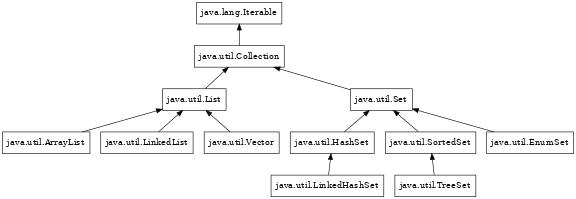
\includegraphics{collection}
\newline

If your method will only iterate over the contents of a collection, the argument type of choice would be \lstinline|java.util.Collection|\autocite{ORACLE_DOC_COLLECTION_INTERFACE}\index{java.util!Collection}. It even allows to add and to remove entries.

The interface \lstinline|java.lang.Iterable|\autocite{ORACLE_DOC_ITERABLE_INTERFACE}\index{java.lang!Iterable} is usually not the proper selection – although it looks like that – because it is also implemented by types like \lstinline|java.nio.file.Path|\autocite{ORACLE_DOC_PATH_INTERFACE}\index{java.nio.file!Path} or \lstinline|java.beans.beancontext.BeanContext|\autocite{ORACLE_DOC_BEANCONTEXT_INTERFACE}\index{java.beans.beancontext!BeanContext}.\footnote{To be precise, \lstinline|Path| and \lstinline|BeanContext| \textit{extend} \lstinline|java.lang.Iterable|, as these are interfaces, too.}

You use the interface \lstinline|java.util.List|\autocite{ORACLE_DOC_LIST_INTERFACE}\index{java.util!List} as the argument type, if somehow the sequence of the entries is important and/or you want to the have duplicate entries in the collection.

The implementations of the interface \lstinline|java.util.Set|\autocite{ORACLE_DOC_SET_INTERFACE}\index{java.util!Set} does not guarantee any particular sequence, but therefore all entries are distinct.

Finally the interface \lstinline|java.util.SortedSet|\autocite{ORACLE_DOC_SORTEDSET_INTERFACE}\index{java.util!SortedSet} allows you to force a particular order of the distinct entries.

The concrete implementations
\begin{itemize}[nosep]
\item{\lstinline|java.util.ArrayList|\autocite{ORACLE_DOC_ARRAYLIST_CLASS}\index{java.util!ArrayList}}
\item{\lstinline|java.util.LinkedList|\autocite{ORACLE_DOC_LINKEDLIST_CLASS}\index{java.util!LinkedList}}
\item{\lstinline|java.util.Vector|\autocite{ORACLE_DOC_VECTOR_CLASS}\index{java.util!Vector}}
\item{\lstinline|java.util.HashSet|\autocite{ORACLE_DOC_HASHSET_CLASS}\index{java.util!HashSet}}
\item{\lstinline|java.util.LinkedHashSet|\autocite{ORACLE_DOC_LINKEDHASHSET_CLASS}\index{java.util!LinkedHashSet}}
\item{\lstinline|java.util.EnumSet|\autocite{ORACLE_DOC_ENUMSET_CLASS}\index{java.util!EnumSet}}
\item{\lstinline|java.util.TreeSet|\autocite{ORACLE_DOC_TREESET_CLASS}\index{java.util!TreeSet}}
\end{itemize}
are rarely used as argument types, with the exception of \lstinline|LinkedHashSet| in cases where you need distinct entries in their insertion order.

The corresponding class hierarchy for a map looks like this:
\index{java.util!Map}\index{java.util!HashMap}\index{java.util!SortedMap}\index{java.util!LinkedHashMap}\index{java.util!Hashtable}\index{java.util!EnumMap}\index{java.util!TreeMap}
\newline
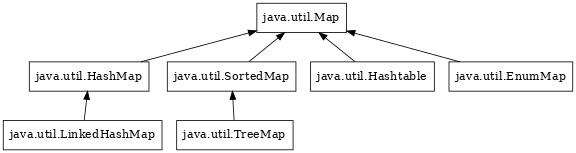
\includegraphics{map}
\newline

In most cases you use \lstinline|java.util.Map|\autocite{ORACLE_DOC_MAP_INTERFACE}\index{java.util!Map} for the type of a method's formal parameter, or \lstinline|java.util.SortedMap|\autocite{ORACLE_DOC_SORTEDMAP_INTERFACE}\index{java.util!SortedMap} if a defined sequence is relevant on iterating over the entries. The concrete implementation \lstinline|java.util.LinkedHashMap|\autocite{ORACLE_DOC_LINKEDHASHMAP_CLASS}\index{java.util!LinkedHashMap} can be used if the insertion order has to be maintained somehow, but the other implementations
\begin{itemize}
\item{\lstinline|java.util.HashMap|\autocite{ORACLE_DOC_HASHMAP_CLASS}\index{java.util!HashMap}}
\item{\lstinline|java.util.Hashtable|\autocite{ORACLE_DOC_HASHTABLE_CLASS}\index{java.util!Hashtable}}
\item{\lstinline|java.util.EnumMap|\autocite{ORACLE_DOC_ENUMMAP_CLASS}\index{java.util!EnumMap}}
\item{\lstinline|java.util.TreeMap|\autocite{ORACLE_DOC_TREEMAP_CLASS}\index{java.util!TreeMap}}
\end{itemize}
are usually not used as argument types.

When using the most general type (the interfaces in case of collection and map) for the arguments types, your methods get a wider range of usability with sacrifying type safety.

All the type discussed here are generic, and you should also consider to use a type variable with them instead of a concrete type if you are not specifically interested in the content type:
\index{java.util!List}
\begin{lstlisting}
public final <T> void myMethod( final List<T> argumentList ) {}
\end{lstlisting}
instead of
\index{java.util!List}
\begin{lstlisting}
// AVOID!
public final void myMethod( final List<Object> argumentList ) {}

// NEVER!
public final void myMethod( final List argumentList ) {}
\end{lstlisting}
For more details refer to chapter \tqfullref{sec:GenericTypes}.
 
%------------------------------------------------------------------------------

\subsubsection{Choose the proper I/O Stream Type}\label{sec:ChooseTheProperIOStreamType}
While the collection types are a clear class hierarchy, this is different for the I/O streams. Basically, there are the (\lstinline|abstract|) classes \lstinline|java.io.InputStream|\autocite{ORACLE_DOC_INPUTSTREAM_CLASS}\index{java.io!InputStream} and \lstinline|java.io.OutputStream|\autocite{ORACLE_DOC_OUTPUTSTREAM_CLASS}\index{java.io!OutputStream}, implementations like \lstinline|java.io.FileInputStream|\autocite{ORACLE_DOC_FILEINPUTSTREAM_CLASS}\index{java.io!FileInputStream} and \lstinline|java.io.FileOutputStream|\autocite{ORACLE_DOC_FILEOUTPUTSTREAM_CLASS}\index{java.io!FileOutputStream}, and classes like \lstinline|java.io.BufferedInputStream|\autocite{ORACLE_DOC_BUFFEREDINPUTSTREAM_CLASS}\index{java.io!BufferedInputStream} and \lstinline|java.io.BufferedOutputStream|\autocite{ORACLE_DOC_BUFFEREDOUTPUTSTREAM_CLASS}\index{java.io!BufferedOutputStream} that are decorators for the implementations, easily to identify because the constructors for the decorators take a stream instance as their arguments.

In most cases you use just the abstract classes as the types for the formal parameters of your methods, in rare cases one of the decorator classes. There are nearly no use cases that would require to use an implementation class like \lstinline|FileInputStream|\index{java.io!FileInputStream} as argument type.

\subsubsection{String vs. CharSequence}
For the type of method and constructor arguments you should prefer \lstinline|java.lang.CharSequence|\autocite{ORACLE_DOC_CHARSEQUENCE_INTERFACE}\index{java.lang!CharSequence} over \lstinline|java.lang.String|\autocite{ORACLE_DOC_STRING_CLASS}\index{java.lang!String}, even if you in fact need a \lstinline|String|: calling \lstinline|toString()|\index{java.lang!Object!toString()} on an instance of \lstinline|String| is a \verb#NOOP# that will be optimised away by the \verb#javac# compiler or by the JIT, but line~3 from the sample below is easier to read than line~5, and the latter does not provide any additional information to the reader.
\index{java.lang!StringBuilder}\index{org.tquadrat.foundation.util!StringUtils!splitString()}
\begin{lstlisting}[numbers=left]
final var buffer = new StringBuilder();
…
final var parts = splitString( buffer );
…
final var parts = splitString( buffer.toString() );
\end{lstlisting}

Of course, there will be always methods that will be called only with \lstinline|String| instances as the arguments, and  never with an instance of \lstinline|CharBuffer|\autocite{ORACLE_DOC_CHARBUFFER_CLASS} or \lstinline|StringBuilder|\autocite{ORACLE_DOC_STRINGBUILDER_CLASS}, just because of the context they are defined in. Then it does not make any sense at all to define the formal parameter as \lstinline|CharSequence|.

\subsection{\lstinline|boolean| Arguments}\label{sec:BooleanArguments}
You should avoid method or constructor signatures that have formal parameters of type \lstinline|boolean|\index{boolean} or \lstinline|java.lang.Boolean|\index{java.lang!Boolean}. A single flag for a setter is acceptable, but something like the constructor below will cause issues:
\begin{lstlisting}[numbers=left]
public final MyClass
{
        /*------------*\
    ====** Attributes **=============================================    
        \*------------*/
    private final boolean m_Flag01;
    private final boolean m_Flag02;
    private final boolean m_Flag03;
    private final boolean m_Flag04;
    private final boolean m_Flag05;
    private final boolean m_Flag06;
    private final boolean m_Flag07;
    private final boolean m_Flag08;
    private final boolean m_Flag09;
    private final boolean m_Flag10;
    
        /*--------------*\
    ====** Constructors **===========================================
        \*--------------*/
    // BAD!!
    public MyClass( final boolean flag01, final boolean flag02, final boolean flag03, final boolean flag04, final boolean flag05, final boolean flag06, final boolean flag07, final boolean flag08, final boolean flag09 final boolean flag10 )
    {
        m_Flag01 = flag01;
        m_Flag02 = flag02;
        m_Flag03 = flag03;
        m_Flag04 = flag04;
        m_Flag05 = flag05;
        m_Flag06 = flag06;
        m_Flag07 = flag07;
        m_Flag08 = flag08;
        m_Flag09 = flag09;
        m_Flag10 = flag10;
    }   //  MyClass()
    
        /*---------*\
    ====** Methods **================================================
        \*---------*/
    public static final void main( final String... args )
    {
        final var instance = new MyClass( true, false, false, true, false, true, false, true, false, false );
    }   //  main()
}
//  class MyClass
\end{lstlisting}
Can you say with a quick look how that \lstinline|MyClass| object is instantiated in line~40? This approach produces code that is definitely bad to read!

An alternative is this approach:
\index{java.util!EnumSet}\index{java.util!EnumSet!of()}\index{java.util!EnumSet!noneOf()}\index{java.util!Set!contains()}\index{org.tquadrat.foundation.lang!Objects!requireNonNullArgument()}
\begin{lstlisting}[numbers=left]
public final MyClass
{
        /*---------------*\
    ====** Inner Classes **==========================================
        \*---------------*/
    public enum Flag
    {
        FLAG01,
        FLAG02,
        FLAG03,
        FLAG04,
        FLAG05,
        FLAG06,
        FLAG07,
        FLAG08,
        FLAG09,
        FLAG10
    }   //  enum Flag    
   
        /*------------*\
    ====** Attributes **=============================================    
        \*------------*/
    private final boolean m_Flag01;
    private final boolean m_Flag02;
    private final boolean m_Flag03;
    private final boolean m_Flag04;
    private final boolean m_Flag05;
    private final boolean m_Flag06;
    private final boolean m_Flag07;
    private final boolean m_Flag08;
    private final boolean m_Flag09;
    private final boolean m_Flag10;
    
        /*--------------*\
    ====** Constructors **===========================================
        \*--------------*/
    public MyClass( final Flag... flags )
    {
        final Set<Flag> flagSet = switch( requireNonNullArgument( flags, "flags" ).length )
        {
            case 0 -> EnumSet.noneOf( Flag.class );
            case 1 -> EnumSet.of( flags [0] );
            default -> EnumSet.of( flags [0], flags );
        }
        m_Flag01 = flagSet.contains( FLAG01 );
        m_Flag02 = flagSet.contains( FLAG02 );
        m_Flag03 = flagSet.contains( FLAG03 );
        m_Flag04 = flagSet.contains( FLAG04 );
        m_Flag05 = flagSet.contains( FLAG05 );
        m_Flag06 = flagSet.contains( FLAG06 );
        m_Flag07 = flagSet.contains( FLAG07 );
        m_Flag08 = flagSet.contains( FLAG08 );
        m_Flag09 = flagSet.contains( FLAG09 );
        m_Flag10 = flagSet.contains( FLAG10 );
    }   //  MyClass()
    
        /*---------*\
    ====** Methods **================================================
        \*---------*/
    public static final void main( final String... args )
    {
        final var instance = new MyClass( FLAG01, FLAG04, FLAG06, FLAG08 );
    }   //  main()
}
//  class MyClass
\end{lstlisting}
That is definitely easier to read than the original version. You should even consider whether you really want to have all the \lstinline|boolean| attributes: you can replace them by an \lstinline|EnumSet|\autocite{ORACLE_DOC_ENUMSET_CLASS}\index{java.util!EnumSet} that holds values of type \lstinline|MyClass.Flag|. A getter is now implemented like in this sample:
\index{java.util!EnumSet}\index{java.util!EnumSet!noneOf()}\index{java.util!Set!add()}\index{java.util!Set!contains()}\index{org.tquadrat.foundation.lang!Objects!requireNonNullArgument()}
\begin{lstlisting}
public final MyClass
{
        /*---------------*\
    ====** Inner Classes **==========================================
        \*---------------*/
    public enum Flag
    {
        …
    }   //  enum Flag    
   
        /*------------*\
    ====** Attributes **=============================================    
        \*------------*/
    private final Set<Flag> m_Flags = EnumSet.noneOf( Flag.class );
    
        /*--------------*\
    ====** Constructors **===========================================
        \*--------------*/
    public MyClass( final Flag... flags )
    {
        for( final flag : requireNonNullArgument( flags, "flags" ) )
        {
            m_Flags.add( flag );
        }
    }   //  MyClass()
    
        /*---------*\
    ====** Methods **================================================
        \*---------*/
    public final boolean isFlag01() { return m_Flags.contains( FLAG01 ) );
        
    public static final void main( final String... args )
    {
        final var instance = new MyClass( FLAG01, FLAG04, FLAG06, FLAG08 );
    }   //  main()
}
//  class MyClass
\end{lstlisting}

%------------------------------------------------------------------------------

\subsection{Multiple Parameters with same Type}\label{sec:MultipleSameTypeArgs}
Chapter \tqref{sec:BooleanArguments} describes the problem that multiple \lstinline|boolean| parameters can cause in a method or constructor signature.

It should be obvious that long parameter lists with only \lstinline|int|, \lstinline|String| or \lstinline|MyClass| arguments (or whatever else~…) will cause the same kind of problems. Therefore you should avoid that kind of signature declarations.

Unfortunately, the solution is not that simple as for \lstinline|boolean| arguments.

For a constructor, you can think about the implementation of the Builder pattern\autocite{Gamma:DesignPatterns}, but that does not work for methods.

Another alternative is described in chapter \tqref{sec:GenericParameterTypes}.

%------------------------------------------------------------------------------

\subsection{Generic Parameter Types}\label{sec:GenericParameterTypes}
The topic of this chapter is closely related to that of chapter \tqfullref{sec:MultipleSameTypeArgs}, and it touches also the topic of parameter validation that is discussed in chapter \tqvref{sec:CheckingMethodParametersAndReturnValues} as well as chapter \tqfullvref{sec:ValueTypes}.

‘Generic parameter type’ means here a type whose values can have multiple meanings: an \lstinline|int| could be a \verb#x# coordinate of a point in a graphic, a color component, the price for something or a day in a month. In the same way, a \lstinline|String| could be text message, an email address or a customer id.

The problem with these that their value does not have a meaning outside a defined context: \lstinline|10| means nothing, but as argument to \lstinline|Thread::sleep|\autocite{ORACLE_DOC_THREAD:sleep}\index{java.lang!Thread!sleep()} is stands for the ten milliseconds that the current thread will be asleep:
\index{java.lang!InterruptedException}
\begin{lstlisting}
try
{
    sleep( 10 );
}
catch( final InterruptedException ignored )
{
    /* Deliberately ignored */
}    
\end{lstlisting}
But in another context, it could be a length, a port number or a magic number\index{magic number}.

First, avoid the use of magic numbers\index{magic number}! Use enums instead! At least use constants if the magic numbers\index{magic number} are defined by an external library.

A sample for that is the class \lstinline|java.sql.Types|\autocite{ORACLE_DOC_TYPES_CLASS}\index{java.sql!Types}: the various SQL types are represented by an integer number. The enum class \lstinline|java.sql.JDBCType|\autocite{ORACLE_DOC_JDBCTYPE_ENUM}\index{java.sql!JDBCType} that was introduced with JDBC~4.2 shows how this could be handled: when calling \lstinline|JDBCType::getVendorTypeNumber|\autocite{ORACLE_DOC_JDBCTYPE:getVendorTypeNumber}\index{java.sql!JDBCType!getVendorTypeNumber()} on a SQL type, it returns the corresponding value from \lstinline|Types|\index{java.sql!Types}, while \lstinline|JDBCType::valueOf|\autocite{ORACLE_DOC_JDBCTYPE:valueOf}\index{java.sql!JDBCType!valueOf()} returns the enum constant for the corresponding integer value from \lstinline|Types|\index{java.sql!Types}.

When using an enum, you also benefit from the strict typing of Java:
\begin{lstlisting}
public void assignDataType( final int type );
\end{lstlisting}
can be called with any integer value; of course you should use one of the constants from \lstinline|Types|\index{java.sql!Types}, but this is not enforced in any way. And the validation whether the given number is allowed is a nightmare.

But when declaring
\index{java.sql!JDBCType}
\begin{lstlisting}
public void assignDataType( final JDBCType type );
\end{lstlisting}
the valid arguments are limited to the values in the enum class, and the argument validation can be reduced to a simple \lstinline|null| check. The compiler will reliably protect you from using an invalid data type~…

But it also it helps to protect your code from other bugs; assume a method with the following method signature:
\begin{lstlisting}
public void assignDataTypeToColumn( final int type, final int columnIndex )
{
    …
}	//	assignDataTypeToColumn()
\end{lstlisting}

The compiler will not complain about this method invocation:
\index{java.sql!Types!BOOLEAN}
\begin{lstlisting}
final var columnIndex = 7;
assignDataTypeToColumn( columnIndex, Types.BOOLEAN );
\end{lstlisting}

But this will not compile until you get the arguments on the method call right:
\index{java.sql!JDBCType}\index{java.sql!JDBCType!BOOLEAN}
\begin{lstlisting}
public void assignDataTypeToColumn( final JDBCType type, final int columnIndex )
{
    …
}   //  assignDataTypeToColumn()

…

final var columnIndex = 7;
// DOES NOT COMPILE!!
assignDataTypeToColumn( columnIndex, JDBCType.BOOLEAN );
\end{lstlisting}
Refer also to chapter \tqfullvref{sec:SwapToCompilerErrors}.

The same kind of bug is this one:
\begin{lstlisting}
public final Order createOrder( final String customerId, final String articleNumber )
{
    …
}   //  createOrder()

…

final var customerId = "C-1234";
final var articleNumber = "BigBook_4711";
final var order = createOrder( articleNumber, customerId );
\end{lstlisting}
You can avoid this easily by defining the domain value types \lstinline|CustomerId| and \lstinline|ArticleNumber| and using them for the formal parameters of \lstinline|createOrder()|; then the compiler will already complain.

A related problem class is this:
\index{java.lang!Thread!sleep()}\index{java.lang!InterruptedException}
\begin{lstlisting}
final var minutes = 10;
try
{
    Thread.sleep( minutes );
}
catch( final InterruptedException ignored )
{
    /* Deliberately ignored */
}
\end{lstlisting}
Do you remember? \lstinline|Thread::sleep| takes the waiting time in milliseconds, not in minutes~…

This class of bugs can be addressed by the definition of ‘value types’ or ‘dimensioned values’\footnote{Although this will not necessary help to prevent providing values with the wrong dimension to already existing methods~…}. 

Value types and domain value types are covered in more detail in chapter \tqvref{sec:ValueTypes}.

%------------------------------------------------------------------------------

\subsection{Arrays and \lstinline|varargs| as Arguments}
The signatures \lstinline|myMethod( final String... args )| (using \verb#vararg#) and \lstinline|myMethod( final String [] args )| are basically the same. There is only a difference on how to call a method with one or the other signature.

The only option for the call to the variant with the array argument signature looks like this:
\begin{lstlisting}
public final void myMethod( final String [] args ) { … }

…

final var args = new String [] { "value1", "value2", … };
myMethod( args ); 
\end{lstlisting}

The \verb#vararg# variant additionally allows to be invoked like this:
\begin{lstlisting}
public final void myMethod( final String... args ) { … }

…

final var args = new String [] { "value1", "value2", … };
myMethod( args ); 

myMethod( "value1", "value2", … );
\end{lstlisting}

The only other difference is that a \verb#vararg# has to be the last formal parameter in a method or constructor signature, while a mere array argument can be anywhere on the parameters list.

Internally, the arguments are represented as arrays in both cases; this means, the body would look identically irrespectively the kind of the formal parameter.

And arrays are not immutable: despite the \lstinline|final| qualifier, I can always assign a new value to an (existing) array element. As a consequence you cannot store just the reference for a provided array to an attribute of your class, you have to copy the array (and if the array elements are also not immutable, it has to be a deep copy). In this regard, arrays are like collections.

For a shallow copy, there are multiple options:
\index{java.lang!Object!clone()}\index{java.lang!System!arraycopy()}\index{java.util!Arrays!copyOf()}\index{java.util!Arrays!stream()}\index{java.util.stream!Stream!toArray()}
\begin{lstlisting}[numbers=left]
public final void myMethod( final String... args )
{
    final var c1 = args.clone();

    final var c2 = new String [args.length];
    System.arraycopy( args, 0, c2, 0, args.length );

    final var c3 = Arrays.copyOf( args, args.length );

    final var c4 = Arrays.stream( args ).toArray( String []::new );
}   // myMethod()
\end{lstlisting}

The Java Runtime library does not provide any pre-build solutions for a deep copy of arrays; if you do not want to implement it yourself, you can look for 3\textsuperscript{rd} libraries  providing the respective functionality.

%------------------------------------------------------------------------------

\section{Types for Return Values}\label{sec:TypesReturnValues}
This topic is relevant for all types of code, not only for code in a public API. Basically, it can be reduced to two questions that needs to be answered:
\begin{enumerate}
\item{Interface vs. concrete Class}
\item{Mutable vs. Immutable}
\end{enumerate}

In general, the answers are “Interface” and “Immutable”, but this is not always the best option.

\subsubsection{Principles}
\begin{enumerate}[label=P\arabic*.]
\item{A return value may not provide access to the internal status of an object.

There are exceptions to this rule, in particular for internal code, but in general it must be taken care that a modification to a returned value does not have an unwanted impact to the status of the object that owned the accessor method.}\label{p:TypesForReturnValues:NoInternalStatus}

\item{Chose the return type based on what the caller may want to do with the return value.

Together with \ref{p:TypesForReturnValues:NoInternalStatus} this can result in return types for accessor methods that are completely unrelated to the types of the associated attributes.}

\item{Avoid to return magic values to indicate errors.

This also means that you should avoid to return \lstinline|null|. We discussed that already in chapter \tqfullref{sec:CheckingMethodParametersAndReturnValues}.}
\end{enumerate}

%------------------------------------------------------------------------------

\subsection{General vs. specific Return Types}\label{sec:ReturnTypes}
Same as for the types of the formal parameters (see chapter \tqfullvref{sec:ArgumentTypes}), the type for a return value of a method should always be the most general type (interface or class) possible, based on the features that the caller might require or expect from the return type. Consequently, \lstinline|java.lang.Object|\index{java.lang!Object} is rarely the correct type for the return value.

This means, you will usually use \lstinline|Collection|\index{java.util!Collection} or \lstinline|List|\index{java.util!List} instead of \lstinline|LinkedList|\index{java.util!LinkedList}, \lstinline|OutputStream|\index{java.io!OutputStream} instead of \lstinline|ByteArrayOutputStream|\autocite{ORACLE_DOC_BYTEARRAYOUTPUTSTREAM_CLASS}\index{java.io!ByteArrayOutputStream}, and so on.

Only when a concrete class or a more specialised interface provides features that are relevant for the caller, the method should be defined to return that type.

One difference is in regard of methods returning strings: here you should \textit{not} use \lstinline|CharSequence|\index{java.lang!CharSequence} as the return type! In nearly all cases where a method returns a string this value will really be an instance of \lstinline|java.lang.String|\autocite{ORACLE_DOC_STRING_CLASS}\index{java.lang!String} anyway – not to mention that \lstinline|String|\index{java.lang!String} implements \lstinline|CharSequence|\index{java.lang!CharSequence}.

Another reason is that the interface \lstinline|CharSequence|\index{java.lang!CharSequence} is implemented by immutable types (link \lstinline|java.lang.String|\index{java.lang!String}) and mutable types (e.g. \lstinline|java.lang.StringBuilder|\index{java.lang!StringBuilder}) as well. Depending on how the caller wants to use the return value, it may have to check for the concrete type first\footnote{…~just to find out that it is a \lstinline|String| in most cases.}.

%------------------------------------------------------------------------------

\subsection{Mutable Return Types}\label{sec:MutableReturnTypes}
In general, it is not evil if a method returns a mutable type, but it can get nasty under some circumstances – for example when you expose the object's internal state this way:
\index{java.util!List}\index{java.util!ArrayList}
\begin{lstlisting}
public final class MyClass
{
    private final List<String> m_Attribute = new ArrayList<>();

    // PROBLEMATIC!!    
    public final List<String> getAttribute() { return m_Attribute; }
}
//  class MyClass    
\end{lstlisting}

This means that code like that below would modify \lstinline|myObject| – and not only the lines~3 to~5, but also the lines~9 to~11:
\index{java.util!List!add()}\index{java.util!List!sort()}\index{java.util!List!clear()}\index{java.lang!String!CASE\_INSENSITIVE\_ORDER}
\begin{lstlisting}[numbers=left]
final var myObject = new MyClass();

myObject.getAttribute().add( "Some String" );
myObject.getAttribute().sort( String.CASE_INSENSITIVE_ORDER );
myObject.getAttritute().clear();

final var list = myObject.getAttribute();

list.add( "Some String" );
list.sort( String.CASE_INSENSITIVE_ORDER );
list.clear();
\end{lstlisting}
Usually, this is not desired! Otherwise, it should be clearly documented: 
\begin{lstlisting}
…
/**
 *  Returns a reference to the attribute.
 * 
 *  @note Any modifications of the returned value will be reflected 
 *      to the attribute itself and changes the state of the object.
 * 
 *  @return The reference to the attribute.
 */ 
public final List<String> getAttribute() { return m_Attribute; }
…
\end{lstlisting}

But keep in mind that changes to the state of the object may be reflected also to the return value if your method returns a reference to a mutable attribute:
\index{java.util!List}\index{java.util!List!add()}\index{java.util!List!sort()}\index{java.util!ArrayList}
\begin{lstlisting}[numbers=left,firstnumber=23]
public final class MyClass
{
    private final List<String> m_Attribute = new ArrayList<>();

    public final void addAttributEntry( final String s )
    {
        m_Attribute.add( s );
    }   //  addAttributeEntry()
    
    // PROBLEMATIC!!    
    public final List<String> getAttribute() { return m_Attribute; }
}
//  class MyClass    

…

final var myObject = new MyClass();
final var list = myObject.getAttribute();
final var size1 = list.size();
myObject.addAttributeEntry( "Some String" );
final var size2 = list.size();

final var status = size1 == size2;
\end{lstlisting}
The value of \lstinline|status| in line~23 will always be \lstinline|false|!

Some better implementations of \lstinline|getAttribute()| would be:
\index{java.util!List}\index{java.util!List!copyOf()}\index{java.util!Collections!unmodifiableList()}\index{java.util!ArrayList}\index{java.lang!Object!clone()}
\begin{lstlisting}[numbers=left]
/**
 *  Returns the attribute.
 * 
 *  @return The attribute.
 */ 
public final List<String> getAttribute() 
{ 
	final var retValue = List.copyOf( m_Attribute );
	
	final List<String> retValue = unmodifiableList( m_Attribute );
	
	final List<> retValue = new ArrayList<>( m_Attribute );
	
	final List<String> retValue = unmodifiableList( new ArrayList<>( m_Attribute ) );
	
	final List<String> retValue = m_Attribute.clone();

    //---* Done *----------------------------------------------------
    return retValue;
}   //  getAttribute()
\end{lstlisting}

\paragraph{Line~8} creates an unmodifiable copy of \lstinline|m_Attribute|. The method \lstinline|copyOf()| exists for \lstinline|java.util.List|\autocite{ORACLE_DOC_LIST:copyOf}\index{java.util!List!copyOf()}, \lstinline|java.util.Set|\autocite{ORACLE_DOC_SET:copyOf}\index{java.util!Set!copyOf()} and \lstinline|java.util.Map|\autocite{ORACLE_DOC_MAP:copyOf}\index{java.util!Map!copyOf()}.

\lstinline|copyOf()| has some limitations: first is that \lstinline|null| is not valid as a value, and – for \lstinline|Map|\index{java.util!Map} – as a key.

Next it is important to know, that \lstinline|Set::copyOf|\index{java.util!Set!copyOf()} returns an implementation of \lstinline|Set|\index{java.util!Set} that resembles a \lstinline|java.util.HashSet|\autocite{ORACLE_DOC_HASHSET_CLASS}\index{java.util!HashSet}, and for \lstinline|Map::copyOf|\index{java.util!Map!copyOf()} the return value is resembling a \lstinline|java.util!HashMap|\autocite{ORACLE_DOC_HASHMAP_CLASS}\index{java.util!HashMap} – this means that any sort order gets lost for the copy.

\paragraph{Line~10} wraps \lstinline|m_Attribute| into an unmodifiable instance of \lstinline|List|\index{java.util.List!copyOf()}. Drawback is that the returned value changes when the attribute itself is modified somehow.

The utility class \lstinline|java.util.Collections|\index{java.util!Collections}\autocite{ORACLE_DOC_COLLECTIONS_CLASS} provides not only the shown method \lstinline|unmodifiableList()|\autocite{ORACLE_DOC_COLLECTIONS:unmodifiableList}\index{java.util!Collections!unmodifiableList()} but also corresponding methods for \lstinline|Collection|\autocite{ORACLE_DOC_COLLECTIONS:unmodifiableCollection}\index{java.util!Collections!unmodifiableCollection()}, \lstinline|Set|\autocite{ORACLE_DOC_COLLECTIONS:unmodifiableSet}\index{java.util!Collections!unmodifiableSet()} and \lstinline|Map|\autocite{ORACLE_DOC_COLLECTIONS:unmodifiableMap}\index{java.util!Collections!unmodifiableMap()}. 

\paragraph{Line~12} creates a instance of \lstinline|java.util.ArrayList|\autocite{ORACLE_DOC_ARRAYLIST_CLASS}\index{java.util!ArrayList} for the return value and initialises that with \lstinline|m_Attribute|. The returned value will be mutable, but changes will not affect the attribute and therefore will not affect the state of the object instance, too. And \lstinline|null| values are no problem, other than for the solution with \lstinline|copyOf()|.

\paragraph{Line~14} basically combines lines~10 and 12, eliminating the shortcoming of the solutions from lines~8 and 10.

\paragraph{Line~16} ‘clones’\index{java.lang!Object!clone()} \lstinline|m_Attribute|; obviously this works only for instances that implement \lstinline|java.lang.Cloneable|\autocite{ORACLE_DOC_CLONEABLE_INTERFACE}\index{java.lang!Cloneable}, but although collections (and arrays) are cloneable themselves, they may contain elements that are not cloneable, causing a \lstinline|CloneNotSupportedException|\autocite{ORACLE_DOC_CLONENOTSUPPORTEDEXCEPTION_CLASS}\index{java.lang!CloneNotSupportException}.\\[1\baselineskip]

Remember that arrays are not immutable; you can always assign a new value to an existing array element. Therefore you have to take the same precautions when your method should return an array attribute as for returning a collection.
\index{java.lang!Object!clone()}\index{java.lang!System!arraycopy()}\index{java.util!Arrays!copyOf()}\index{java.util!Arrays!stream()}\index{java.util.stream!Stream!toArray()}
\begin{lstlisting}[numbers=left]
public final class MyClass
{
    private String [] m_Attribute;

    /**
     *  Returns the attribute.
     * 
     *  @return The attribute.
     */ 
    public final String [] getAttribute()
    {
        final var retValue = m_Attribute.clone();

        final var retValue = new String [m_Attribute.length];
        System.arraycopy( m_Attribute, 0, retValue, 0, m_Attribute.length );

        final var retValue = Arrays.copyOf( m_Attribute, m_Attribute.length );

        final var retValue = Arrays.stream( m_Attribute )
            .toArray( String []::new );

        //---* Done *------------------------------------------------
        return retValue;
    }   // getAttribute()
}
//  class MyClass    
\end{lstlisting}

In the examples, the element type for both, the collections and the arrays, is immutable\footnote{\lstinline|java.lang.String|\index{java.lang!String} is immutable.}; if the elements would be mutable, you need to take the corresponding precautions for them, too. Basically that would mean a deep copy of the collection or the array.

In general you have to take care that you will not return a reference to an attribute with a mutable type that would allow to modify the internal state of the owning object. This clearly does not affect just collections – although this is the most common case – but for example also instances of \lstinline|java.util.Date|\autocite{ORACLE_DOC_DATE_CLASS}\index{java.util!Date}\footnote{Another good reason to abandon \lstinline|java.util.Date| and to use the classes from the \lstinline|java.time|\autocite{ORACLE_DOC_TIME_PACKAGE}\index{java.time} package instead.}. Obviously, for other types the details on how to create a copy or to make them immutable will differ.

If a method creates (generates, obtains, reads, loads,~…) the value it returns, it is part of the methods's contract whether that value is mutable or not.

%------------------------------------------------------------------------------

\subsection{Special Return Values}\label{sec:SpecialReturnValues}
‘Special return values’ here does not mean those ‘magic numbers’\index{magic number} mentioned in chapter \tqvref{sec:GenericParameterTypes} and elsewhere, although you should avoid them as return values in the same way as you should not use them as arguments to a method call.

This term indicates otherwise impossible return values indicating a special condition, like in the samples below:
\index{java.lang!String!indexOf()}\index{java.lang!String!substring()}\index{java.util!Map}\index{java.util!Map!get()}
\begin{lstlisting}[numbers=left]
final var input = "Some Text follows …";
final var pos = input.indexOf( "value" );
if( index > 0 ) process( input.substring( 0, pos ) );

final Map<Key,Value> map = loadData();
final var key = getKey();
final var value = map.get( key );
if( nonNull( value ) ) process( value );
\end{lstlisting}
In line~2, the method \lstinline|String::indexOf|\autocite{ORACLE_DOC_STRING:indexOf}\index{java.lang!String!indexOf()} return \verb#-1# in case the given text is not part of the \lstinline|String|.

In the same way, the method \lstinline|Map::get|\autocite{ORACLE_DOC_MAP:get}\index{java.util!Map!get()} in line~7 returns \lstinline|null| if the given key is not in the map. Unfortunately, \lstinline|null| could also be a valid value, so in this case it does not necessarily indicate that key is not in the map.

You should avoid this kind of return values.

A better declaration for the two methods would be\footnote{Both methods had been part of the Java Runtime library since version~1.0, and no one seriously suggests to change them now; this is just to illustrate the topic.}:
\index{java.lang!String}\index{java.lang!String!indexOf()}\index{java.util!Map}\index{java.util!Map!get()}\index{java.util!Optional}\index{java.util!OptionalInt}
\begin{lstlisting}
public interface Map<K,V>
{
    public Optional<V> get( final K key );
}   //  interface Map

public final class String
{
    public OptionalInt indexOf( final String str ) { … }
}   //  class String
\end{lstlisting}

With this declarations, you could now write the examples from above as:
\index{java.util!Optional}\index{java.util!Optional!ifPresent()}\index{java.util!OptionalInt}\index{java.util!OptionalInt!ifPresent()}
\begin{lstlisting}[numbers=left]
final var input = "Some Text follows …";
final OptionalInt pos = input.indexOf( "value" );
pos.ifPresent( p -> process( input.substring( 0, p ) ) ;

final Map<Key,Value> map = loadData();
final var key = getKey();
final Optional<Value> value = map.get( key );
value.ifPresent( this::process );
\end{lstlisting}

The classes \lstinline|java.util.OptionalInt|\autocite{ORACLE_DOC_OPTIONALINT_CLASS}\index{java.util.OptionalInt}, \lstinline|java.util.OptionalLong|\autocite{ORACLE_DOC_OPTIONALLONG_CLASS}\index{java.util.OptionalLong} and \lstinline|java.util.OptionalDouble|\autocite{ORACLE_DOC_OPTIONALDOUBLE_CLASS}\index{java.util.OptionalDouble} can help you to avoid “magic numbers”\index{magic number} as return values, indicating special results.

In cases were \lstinline|null| seemed the proper response, choose \lstinline|java.util.Optional|\autocite{ORACLE_DOC_OPTIONAL_CLASS}\index{java.util.Optional} instead.

So you can implement the methods in your code they \textit{never} return \lstinline|null| nor a magic number\index{magic number} of some kind. Nevertheless, when you are implementing a (3\textsuperscript{rd} party) interface that requests a return value of \lstinline|null| or another special value under some conditions, you have to obey that requirements.

In Java, you usually do not return an error code if an operation fails – that \lstinline|Map::get| returns \lstinline|null| if the key is not mapped is not indicating an error: that a key is not mapped is one expected result. So instead of returning an error code, a method will throw an exception.

But what if you do not want to throw an exception, for whatever reason?

Try this:
\index{java.util!Optional}\index{java.util!Optional!ofNullable()}\index{org.tquadrat.foundation.lang!Objects!requireNonNullArgument()}
\begin{lstlisting}[numbers=left,caption={Status Record}]
public record Status( ResultCode resultCode, Optional<Data> data )
{
        /*---------------*\
    ====** Inner Classes **==========================================
        \*---------------*/
    /** */
    public enum ResultCode
    {
        SUCCESS, NO_DATA, FAILURE, TIMEOUT, INCOMPLETE
    }
    //  enum ResultCode
    
        /*--------------*\
    ====** Constructors **===========================================
        \*--------------*/
    public Status( final ResultCode resultCode, final Data data )
    {
        this( resultCode, Optional.ofNullable( data ) );
    }   //  Status()

    public Status( final ResultCode resultCode, final Optional<Data> data )
    {
        this.resultCode = requireNonNullArgument( resultCode, "resultCode" );
        this.data = requireNonNullArgument( data, "data" );
    }   //  Status()
}
//  record Status
\end{lstlisting}

This would allow you to write:
\index{java.util!Optional!ifPresent()}
\begin{lstlisting}
public final Status retrieveData() { … }
…
var proceed = true;
while( proceed )
{
    final var status = retrieveData();
    switch( status.resultCode )
    {
        case SUCCESS -> process( status.data().get() );
        case INCOMPLETE -> status.data().ifPresent( this::processIncomplete );
        case NO_DATA -> proceed = false;
        case TIMEOUT -> reconnect();
        case FAILURE -> throw new ProcessStatusException();
        default -> throw new UnsupportedEnumError( status.resultCode() );
    }
\end{lstlisting}

If you need this kind of return values more often for your project, you can enhance that \lstinline|Status| class in various ways. So you can use a type variable instead of the concrete class \lstinline|Data|, to make the class generic. Or you add a method like this:
\begin{lstlisting}
…
public final void onSuccess( final Consumer<Data> processor )
{
    if( resultCode == SUCCESS ) data.ifPresent( processor::accept );
}   //  onSuccess()
…
\end{lstlisting}

%------------------------------------------------------------------------------

\section{Local Variable Type Inference}\label{sec:LocalVariableTypeInference}
Java~10 introduced type inference for local variables. Previously, all local variable declarations required an explicit (manifest) type on the left-hand side. With type inference, the explicit type can be replaced by the reserved type name \lstinline|var|\footnote{That \lstinline|var| was not introduced as an new \textit{keyword} for the language means it can be still used as name for local variables, fields and methods – although it is definitely discouraged to do so!} for local variable declarations that have initialisers. The type of the variable is inferred from the type of the initialiser:
\begin{lstlisting}
final var s = "String";                   // s is java.lang.String
final var i = 9;                          // i is int
final var d = 3.1415;                     // d is double
final var list = new ArrayList<String>(); // list is java.util.ArrayList<String>
\end{lstlisting}

There is a certain amount of controversy over this feature. Some welcome the concision it enables; others fear that it deprives readers of important type information, impairing readability. And both groups are right, to some extent. It can make code more readable by eliminating redundant information, and it can also make code less readable by eliding useful information. Another group worries that it will be overused, resulting in more bad Java code being written. This is also true, but it’s also likely to result in more good Java code being written. Like all features, it must be used with judgement. There’s no blanket rule for when it should and shouldn’t be used. 

Local variable declarations do not exist in isolation; the surrounding code can affect or even overwhelm the effects of using \lstinline|var|. The goal of this chapter is to examine the impact that surrounding code has on \lstinline|var| declarations, to explain some of the tradeoffs, and to provide guidelines for the effective use of \lstinline|var|.\footnote{This chapter is basically a summary of the article “Local Variable Type Inference – Style Guidelines”, published by Stuart~W.~Marks in March 2018\autocite{Marks:LocalVariableTypeInference}.}

\subsubsection{Principles}
\begin{enumerate}[label=P\arabic*.]
\item{Reading code is more important than writing code.

Code is read much more often than it is written. Further, when writing code, you usually have the whole context in your head, and take your time; when reading code, you are often context-switching, and may be in more of a hurry. Whether and how particular language features are used ought to be determined by their impact on future readers of the program, not its original author. Shorter programs can be preferable to longer ones, but shortening a program too much can omit information that is useful for understanding the program. The central issue here is to find the right size for the program such that understandability is maximized.

You should be specifically unconcerned here with the amount of keyboarding that is necessary to input or to edit a program. While concision may be a nice bonus for the author, focusing on it misses the main goal, which is to improve the understandability of the resulting program.}

\item{Code should be clear from local reasoning.

The reader should be able to look at a \lstinline|var| declaration, along with uses of the declared variable, and understand almost immediately what is going on. Ideally, the code should be readily understandable using only the context from a snippet or a patch. If understanding a \lstinline|var| declaration requires the reader to look at several locations around the code, it might not be a good situation in which to use \lstinline|var|. Then again, it might indicate a problem with the code itself.}

\item{Code readability shouldn’t depend on IDEs.

Code is often written and read within an IDE, so it’s tempting to rely heavily on the code analysis features of IDEs. For type declarations, why not just use \lstinline|var| everywhere, since one can always point at a variable to determine its type?

The main reason is that code is often read outside an IDE. Code appears in many places where IDE facilities are not available, such as snippets within a document, browsing a repository on the internet, or in a patch file. It is counterproductive to have to import code into an IDE simply to understand what the code does.

Code should be self-revealing. It should be understandable on its face, without the need for assistance from tools.}

\item{Explicit types are a tradeoff.

Java has historically required local variable declarations to include the type explicitly. While explicit types can be very helpful, they are sometimes not very important, and are sometimes just in the way. Requiring an explicit type can add clutter that crowds out useful information.

Omitting an explicit type can reduce clutter, but only if its omission does not impair understandability. The type is not the only way to convey information to the reader. Other means include the variable's name and the initialiser expression. You should take all the available channels into account when determining whether it is appropriate to mute one of these channels.}
\end{enumerate}

%------------------------------------------------------------------------------
\hrulefill\newpage 
\section{-------------------------------------------- Proceed from here!}
\lipsum[1]

%\subsubsection{Principles}
\begin{enumerate}[label=P\arabic*.]
\item{one}
\item{two}
\item{three}
\end{enumerate}

\begin{itemize}[nosep]
\item{one}
\item{two}
\item{three}
\end{itemize}

\begin{lstlisting}[numbers=left]
\end{lstlisting}
%------------------------------------------------------------------------------

\subsection{Guidelines}
\begin{enumerate}
\item[G1.]{Choose variable names that provide useful information.

This is good practice in general, but it is much more important in the context of \lstinline|var|. In a \lstinline|var| declaration, information about the meaning and use of the variable can be conveyed using the variable's name. Replacing an explicit type with \lstinline|var| should often be accompanied by improving the variable name.

For example:

\begin{lstlisting}
// BAD
final List<Customer> x = dbConnection.executeQuery( query );

// BETTER
final var customerList = dbConnection.executeQuery( query );
\end{lstlisting}

In this case, a useless variable name has been replaced with a name that is evocative of the type of the variable, which is now implicit in the var declaration.

Encoding the variable's type in its name, taken to its logical conclusion, results in “Hungarian Notation”. Just as with explicit types, this is sometimes helpful, and sometimes just clutter. In this example the name \lstinline|customerList| implies that a \lstinline|List| is being returned. That might not be significant. Instead of the exact type, it’s sometimes better for a variable’s name to express the role or the nature of the variable, such as \lstinline|customers|:

\begin{lstlisting}
// BAD
try( final Stream<Customer> result = dbConnection.executeQuery( query ) ) 
{
    return result.map( … )
        .filter( … )
        .findAny();
}

// BETTER
try( final var customers = dbConnection.executeQuery( query ) ) 
{
    final var retValue = customers.map( … )
        .filter( … )
        .findAny();
    return retValue;
}
\end{lstlisting}}

\item[G2.]{Minimize the scope of local variables.

Limiting the scope of local variables is good practice in general. This practice is described in “Effective Java (3\textsuperscript{rd} Edition)”\autocite{Bloch:EffectiveJava}, Item~57. It applies with extra force if \lstinline|var| is in use.

In the following example, the \lstinline|add()| method clearly adds the special item as the last list element, so it’s processed last, as expected.

\begin{lstlisting}
final var items = new ArrayList<Item>( … );
items.add( MUST_BE_PROCESSED_LAST );
for( final var item : items ) { … }
\end{lstlisting}

Now suppose that in order to remove duplicate items, you modify this code to use a \lstinline|HashSet| instead of an \lstinline|ArrayList|, like below:

\begin{lstlisting}
final var items = new HashSet<Item>( … );
items.add( MUST_BE_PROCESSED_LAST );
for( fnial var item : items ) { … }
\end{lstlisting}

Your code now has a bug, since sets do not have a defined iteration order. However, it is likely that you will fix this bug immediately, as the uses of the \lstinline|items| variable are adjacent to its declaration.

Now suppose that this code is part of a large method, with a correspondingly large scope for the \lstinline|items| variable:

\begin{lstlisting}
final var items = new HashSet<Item>( … );

// … 100 lines of code …

items.add( MUST_BE_PROCESSED_LAST );
for( final var item : items ) { … }
\end{lstlisting}

The impact of changing from an \lstinline|ArrayList| to a \lstinline|HashSet| is no longer readily apparent, since \lstinline|items| is used so far away from its declaration. It seems likely that this bug could survive for much longer.

If \lstinline|items| had been declared explicitly as \lstinline|List<String>|, changing the initialiser would also require changing the type to \lstinline|Set<String>|. This \textit{might} prompt you to inspect the rest of the method for code that would be impacted by such a change (then again, it might not). Use of \lstinline|var| would remove this prompting, possibly increasing the risk of a bug being introduced in code like this.

This might seem like an argument against using \lstinline|var|, but it really is not. The initial example that uses \lstinline|var| is perfectly fine. The problem only occurs when the variable's scope is large. Instead of simply avoiding \lstinline|var| in these cases, you should change the code to reduce the scope of the local variables, and only then declare them with \lstinline|var|.}

\item[G3.]{Consider \lstinline|var| when the initialiser provides sufficient information to the reader.

Local variables are often initialised with constructors. The name of the class being constructed is often repeated as the explicit type on the left-hand side. If the type name is long, use of \lstinline|var| provides concision without loss of information:

\begin{lstlisting}
// ACCEPTABLE
final ByteArrayOutputStream outputStream = new ByteArrayOutputStream();

// BETTER
final var outputStream = new ByteArrayOutputStream();
\end{lstlisting}

It is also reasonable to use \lstinline|var| in cases where the initialiser is a method call, such as a \lstinline|static| factory method, instead of a constructor, and when its name contains enough type information:

\begin{lstlisting}
// ACCEPTABLE
final BufferedReader reader = Files.newBufferedReader( … );
final List<String> stringList = List.of("a", "b", "c");

// BETTER
final var reader = Files.newBufferedReader(...);
final var stringList = List.of("a", "b", "c");
\end{lstlisting}

In these cases, the methods names strongly imply a particular return type, which is then used for inferring the type of the variable.}

\item[G4.]{Use \lstinline|var| to break up chained or nested expressions with local variables.

Consider code that takes a collection of strings and finds the string that occurs most often. This might look like the following:

\begin{lstlisting}
return strings.stream()
    .collect( groupingBy( s -> s, counting() ) )
    .entrySet()
    .stream()
    .max( Map.Entry.comparingByValue() )
    .map( Map.Entry::getKey );
\end{lstlisting}

This code is correct, but it is potentially confusing, as it looks like a single stream pipeline. In fact, it’s a short stream, followed by a second stream over the result of the first stream, followed by a mapping of the \lstinline|Optional| result of the second stream. The most readable way to express this code would have been as two or three statements; first group entries into a map, then reduce over that map, then extract the key from the result (if present), as shown below:

\begin{lstlisting}
// BETTER READABLE
final Map<String, Long> freqMap = strings.stream()
    .collect(groupingBy( s -> s, counting() ) );
final Optional<Map.Entry<String,Long>> maxEntryOpt = freqMap.entrySet()
    .stream()
    .max( Map.Entry.comparingByValue() );
return maxEntryOpt.map( Map.Entry::getKey );
\end{lstlisting}

But you probably resisted doing that because writing the types of the intermediate variables seemed too burdensome, so instead they distorted the control flow. Using \lstinline|var| here allows you to express the code more naturally without paying the high price of explicitly declaring the types of the intermediate variables:

\begin{lstlisting}
// EVEN BETTER READABLE
final var freqMap = strings.stream()
    .collect( groupingBy( s -> s, counting() ) );
final var maxEntryOpt = freqMap.entrySet()
    .stream()
    .max( Map.Entry.comparingByValue() );
final var retValue = maxEntryOpt.map( Map.Entry::getKey );
return retValue;
\end{lstlisting}

You might legitimately prefer the first snippet with its single long chain of method calls. However, in some cases it is better to break up long method chains. Using \lstinline|var| for these cases is a viable approach, whereas using full declarations of the intermediate variables as in the second snippet makes it an unpalatable alternative. As with many other situations, the correct use of \lstinline|var| might involve both taking something out (explicit types) and adding something back (better variable names, better structuring of code).}

\subsection{-------------------------------------------- Proceed from here!}
\item[G5.]{Don’t worry too much about “programming to the interface” with local variables.

A common idiom in Java programming is to construct an instance of a concrete type but to assign it to a variable of an interface type. This binds the code to the abstraction instead of the implementation, which preserves flexibility during future maintenance of the code. For example:

\begin{lstlisting}
// ORIGINAL
List<String> list = new ArrayList<>();
If var is used, however, the concrete type is inferred instead of the interface:

// Inferred type of list is ArrayList<String>
var list = new ArrayList<String>();
\end{lstlisting}

It must be reiterated here that var can only be used for local variables. It cannot be used to infer field types, method parameter types, and method return types. The principle of “programming to the interface” is still as important as ever in those contexts.

The main issue is that code that uses the variable can form dependencies on the concrete implementation. If the variable’s initialiser were to change in the future, this might cause its inferred type to change, causing errors or bugs to occur in subsequent code that uses the variable.

If, as recommended in guideline G2, the scope of the local variable is small, the risks from “leakage” of the concrete implementation that can impact the subsequent code are limited. If the variable is used only in code that’s a few lines away, it should be easy to avoid problems or to mitigate them if they arise.

In this particular case, ArrayList only contains a couple of methods that aren’t on List, namely ensureCapacity and trimToSize. These methods don’t affect the contents of the list, so calls to them don’t affect the correctness of the program. This further reduces the impact of the inferred type being a concrete implementation rather than an interface.}
\item[G6.]{Take care when using var with diamond or generic methods.

Both var and the “diamond” feature allow you to omit explicit type information when it can be derived from information already present. Can you use both in the same declaration?

Consider the following:

\begin{lstlisting}
PriorityQueue<Item> itemQueue = new PriorityQueue<Item>();
\end{lstlisting}
This can be rewritten using either diamond or var, without losing type information:

\begin{lstlisting}
// OK: both declare variables of type PriorityQueue<Item>
PriorityQueue<Item> itemQueue = new PriorityQueue<>();
var itemQueue = new PriorityQueue<Item>();
\end{lstlisting}

It is legal to use both var and diamond, but the inferred type will change:

\begin{lstlisting}
// DANGEROUS: infers as PriorityQueue<Object>
var itemQueue = new PriorityQueue<>();
\end{lstlisting}

For its inference, diamond can use the target type (typically, the left-hand side of a declaration) or the types of constructor arguments. If neither is present, it falls back to the broadest applicable type, which is often Object. This is usually not what was intended.

Generic methods have employed type inference so successfully that it’s quite rare for programmers to provide explicit type arguments. Inference for generic methods relies on the target type if there are no actual method arguments that provide sufficient type information. In a var declaration, there is no target type, so a similar issue can occur as with diamond. For example,

\begin{lstlisting}
// DANGEROUS: infers as List<Object>
var list = List.of();
\end{lstlisting}

With both diamond and generic methods, additional type information can be provided by actual arguments to the constructor or method, allowing the intended type to be inferred. Thus,

\begin{lstlisting}
// OK: itemQueue infers as PriorityQueue<String>
Comparator<String> comp = ... ;
var itemQueue = new PriorityQueue<>(comp);

// OK: infers as List<BigInteger>
var list = List.of(BigInteger.ZERO);
\end{lstlisting}

If you decide to use var with diamond or a generic method, you should ensure that method or constructor arguments provide enough type information so that the inferred type matches your intent. Otherwise, avoid using both var with diamond or a generic method in the same declaration.}
\item[G7.]{Take care when using var with literals.
Primitive literals can be used as initialisers for var declarations. It’s unlikely that using var in these cases will provide much advantage, as the type names are generally short. However, var is sometimes useful, for example, to align variable names.

There is no issue with boolean, character, long, and string literals. The type inferred from these literals is precise, and so the meaning of var is unambiguous:

\begin{lstlisting}
// ORIGINAL
boolean ready = true;
char ch = '\ufffd';
long sum = 0L;
String label = "wombat";

// GOOD
var ready = true;
var ch    = '\ufffd';
var sum   = 0L;
var label = "wombat";
\end{lstlisting}

Particular care should be taken when the initialiser is a numeric value, especially an integer literal. With an explicit type on the left-hand side, the numeric value may be silently widened or narrowed to types other than int. With var, the value will be inferred as an int, which may be unintended.

\begin{lstlisting}
// ORIGINAL
byte flags = 0;
short mask = 0x7fff;
long base = 17;

// DANGEROUS: all infer as int
var flags = 0;
var mask = 0x7fff;
var base = 17;
\end{lstlisting}

Floating point literals are mostly unambiguous:

\begin{lstlisting}
// ORIGINAL
float f = 1.0f;
double d = 2.0;

// GOOD
var f = 1.0f;
var d = 2.0;
\end{lstlisting}

Note that float literals can be widened silently to double. It is somewhat obtuse to initialise a double variable using an explicit float literal such as 3.0f, however, cases may arise where a double variable is initialised from a float field. Caution with var is advised here:

\begin{lstlisting}
// ORIGINAL
static final float INITIAL = 3.0f;
...
double temp = INITIAL;

// DANGEROUS: now infers as float
var temp = INITIAL;
\end{lstlisting}

(Indeed, this example violates guideline G3, because there isn’t enough information in the initialiser for a reader to see the inferred type.)}
\end{enumerate}

\subsection{Examples}
This section contains some examples of where var can be used to greatest benefit.

The following code removes at most max matching entries from a Map. Wildcarded type bounds are used for improving the flexibility of the method, resulting in considerable verbosity. Unfortunately, this requires the type of the Iterator to be a nested wildcard, making its declaration more verbose. This declaration is so long that the header of the for-loop no longer fits on a single line, making the code even harder to read.

\begin{lstlisting}
// ORIGINAL
void removeMatches(Map<? extends String, ? extends Number> map, int max) {
    for (Iterator<? extends Map.Entry<? extends String, ? extends Number>> iterator =
             map.entrySet().iterator(); iterator.hasNext();) {
        Map.Entry<? extends String, ? extends Number> entry = iterator.next();
        if (max > 0 && matches(entry)) {
            iterator.remove();
            max--;
        }
    }
}
\end{lstlisting}
Use of var here removes the noisy type declarations for the local variables. Having explicit types for the Iterator and Map.Entry locals in this kind of loop is largely unnecessary. This also allows the for-loop control to fit on a single line, further improving readability.

\begin{lstlisting}
// GOOD
void removeMatches(Map<? extends String, ? extends Number> map, int max) {
    for (var iterator = map.entrySet().iterator(); iterator.hasNext();) {
        var entry = iterator.next();
        if (max > 0 && matches(entry)) {
            iterator.remove();
            max--;
        }
    }
}
\end{lstlisting}

Consider code that reads a single line of text from a socket using the try-with-resources statement. The networking and I/O APIs use an object wrapping idiom. Each intermediate object must be declared as a resource variable so that it will be closed properly if an error occurs while opening a subsequent wrapper. The conventional code for this requires the class name to be repeated on the left and right sides of the variable declaration, resulting in a lot of clutter:

\begin{lstlisting}
// ORIGINAL
try (InputStream is = socket.getInputStream();
     InputStreamReader isr = new InputStreamReader(is, charsetName);
     BufferedReader buf = new BufferedReader(isr)) {
    return buf.readLine();
}
\end{lstlisting}
Using var reduces the noise considerably:

\begin{lstlisting}
// GOOD
try (var inputStream = socket.getInputStream();
     var reader = new InputStreamReader(inputStream, charsetName);
     var bufReader = new BufferedReader(reader)) {
    return bufReader.readLine();
}
\end{lstlisting}

Conclusion
Using var for declarations can improve code by reducing clutter, thereby letting more important information stand out. On the other hand, applying var indiscriminately can make things worse. Used properly, var can help improve good code, making it shorter and clearer without compromising understandability.

%------------------------------------------------------------------------------

\section{Value Types}\label{sec:ValueTypes}

%------------------------------------------------------------------------------
\hrulefill\newpage 
\section{-------------------------------------------- Proceed from here!}
\lipsum[1]

%\subsubsection{Principles}
\begin{enumerate}[label=P\arabic*.]
\item{one}
\item{two}
\item{three}
\end{enumerate}

\begin{itemize}[nosep]
\item{one}
\item{two}
\item{three}
\end{itemize}

\begin{lstlisting}[numbers=left]
\end{lstlisting}
%------------------------------------------------------------------------------

%------------------------------------------------------------------------------

\section{Generics}\label{sec:GenericTypes}

%------------------------------------------------------------------------------
\hrulefill\newpage 
\section{-------------------------------------------- Proceed from here!}
\lipsum[1]

%\subsubsection{Principles}
\begin{enumerate}[label=P\arabic*.]
\item{one}
\item{two}
\item{three}
\end{enumerate}

\begin{itemize}[nosep]
\item{one}
\item{two}
\item{three}
\end{itemize}

\begin{lstlisting}[numbers=left]
\end{lstlisting}
%------------------------------------------------------------------------------

%------------------------------------------------------------------------------

%------------------------------------------------------------------------------



















































\section{Access to Properties}
Encapsulation is an important design principle for classes. This means that the internal state of an object can be manipulated only in a well defined manner, through the methods. Consequently, it may not be possible to modify the attributes  directly, by a direct assignment.

To achieve that, instance or class variables – also known as properties, attributes or fields – have to be \lstinline|private|.

If it is necessary to set or retrieve an instance variable (a property) directly, it mandatory to provide the appropriate methods for this (setter and/or getter, or mutator and/or accessor methods). But often attributes are set or retrieved as a side effect of method calls that modify the internal state of the object instance, or rely on it.

Programmers are inclined to use \lstinline|public| fields when the need a data structure like a \lstinline|struct| in C/C++, and not a full-fledged class. But as Java does not now that data structure, it seems to be a quick solution to have a \lstinline|class| with only \lstinline|public| fields and no methods, just to spare typing effort, and sometimes with the idea, that the direct access to the \lstinline|public| field is much faster that accessing it through a method. But modern optimising compilers will inline the code of a simple getter method, so that there is no difference in the end.

And if you want to avoid the typing, use a \lstinline|record|\autocite{ORACLE_DOC_RECORD,ORACLE_DOC_LANGUAGE_SPECIFICATION:RecordClasses} instead. Sometimes also an instance of \lstinline|java.util.Map| or another collection implementation could be an alternative to a specialised class.
 
Sometimes fields from base classes are defined as \lstinline|protected|, to make them directly accessible by methods from the derived implementations, but this is also discouraged.\footnote{The idea behind that is the same false assumption that the direct access to the \lstinline|protected| field is much faster that accessing it through a method.}

It does not matter if we talk about properties (instance variables) or \lstinline|static| field (class variables): both should always be \lstinline|private|.

Constants are the only exception, obviously, because a constant is explicitly defined as a \lstinline|public static final| field.

Regarding encapsulation in general, refer to chapter \tqvref{sec:EncapsulationWithModules}.

\section{Accessing Fields or Methods using Reflection}\label{sec:Reflection}
First of all, you should avoid to use Reflection whenever possible. Just do not use it!\footnote{The only acceptable exception is for unit tests; we will discuss that later in this chapter.}

One reason is that accessing a field or a method via reflection causes some overhead that decreases a program’s performance. 

Next, such code is usually not easy to read or to understand, not only because of all the necessary error handling code around it.

And with modularisation, it is quite often not even possible to access methods and fields of an object via Reflection, even if they are \lstinline|public|; they are not even visible in some cases.

Of course, there are some patterns whose implementation in Java requires the use of Reflection, because any other approach is either even less performant, much more cumbersome, or will not work at all – meaning there are occasions when it is not really possible to avoid the use of Reflection. Nevertheless, you should still consider an alternative; lambdas\autocite{ORACLE_DOC_LANGUAGE_SPECIFICATION:LambdaExpressions} and method references\autocite{ORACLE_DOC_LANGUAGE_SPECIFICATION:MethodReference} are quite often a very good replacement for an implementation based on Reflection.

Reflection also allows you to access non-\lstinline|public| member of a class that are usually not accessible by your code. This is considered a “dirty hack” and may not be used in production code. In particular as it may not work properly with modules.

But there are useful applications for this, too: you can and should used it in unit tests for \lstinline|private| or \lstinline|protected| methods that are not \lstinline|public| for good reasons, and if these methods cannot be tested indirectly.\footnote{The alternative would be to make the method at least \lstinline|protected|, but this would make it (more) visible to the consumers of the API, and perhaps even accessible – but there was a reason why that method was originally \lstinline|private|.}

I recommend to use the following pattern if you want to access a \lstinline|private| method in your unit tests; first the class under test:
\index{java.lang!String}\index{java.lang!CharSequence}\index{java.io!IOException}
\begin{lstlisting}
public final class MyClass
{
    /**
     *  Does something.
     *
     *  @param  value   The value.
     *  @return The result.
     *  @throws IOException Something went wrong.
     */
    private final String myMethod( final CharSequence value ) throws IOException
    { 
        final var retValue = … 
        
        //---* Done *------------------------------------------------
        return retValue;
    }   //  myMethod()
}   
//  class MyClass
\end{lstlisting}
The test class:
\index{java.lang!String}\index{java.lang!CharSequence}\index{java.io!IOException}\index{java.lang!Class!getDeclaredMethod()}\index{java.lang.reflect.Method!setAccessible()}\index{java.lang.reflect.Method!invode()}\index{java.lang!NoSuchMethodException}\index{java.lang!ExceptionInInitialiserError}\index{java.lang!String!formatted()}\index{org.tquadrat.foundation.lang!requiredNonNullArgument()}\index{java.lang!IllegalAccessException}\index{java.lang.reflect!InvocationTargetException}\index{java.lang!ClassCastException}\index{java.lang!AssertionError}\index{java.lang.Throwable!getCause()}\index{ org.junit.jupiter.api!Assertions!assertTrue()}
\begin{lstlisting}[numbers=left]
/**
 *  This class provides some unit tests for
 *  {@link MyClass}.
 */
public final class TestMyClass
{
        /*------------------------*\
    ====** Static Initialisations **=================================
        \*------------------------*/
    /**
     *  The reference to {@code myMethod()}.
     */
    private static final Method METHOD_myMethod;
    
    static
    {
        final var targetClass = MyClass.class;
        String methodName;
        try
        {
            methodName = "myMethod";
            METHOD_myMethod = targetClass.getDeclaredMethod( methodName, CharSequence.class );
            METHOD_myMethod.setAccessible( true );
        }
        catch( final NoSuchMethodException ignored )
        {
            throw new ExceptionInInitializerError( "Cannot find method '%s()' in class '%s'".formatted( methodName, targetClass.getName() );
        }
    }
    
        /*---------*\
    ====** Methods **================================================ 
        \*---------*/
    /**
     *  Calls
     *  {@link MyClass#myMethod(CharSequence)}
     *
     *  @param  instance    The candidate.
     *  @param	value   The value.
     *  @return The result.
     *  @throws IOException Something went wrong.
     */
    protected static final String myMethod( final MyClass instance, final CharSequence value )
    {
        final String retValue;
        try
        {
            retValue = (String) METHOD_myMethod.invoke( requireNonNullArgument( instance, "instance" ), value );
        }
        catch( final IllegalAccessException | ClassCastException e )
        {
            throw new AssertionError( e );
        }
        catch( final InvocationTargetException e )
        {
            switch( e.getCause() )
            {
                case null -> throw new AssertionError( e );
                case IOException ioe -> throw ioe;
                default -> throw new AssertionError( e.getCause() );
            }
        }
    }   //  myMethod()   
    
    @Test
    final void testMyMethod() throws Exception
    {
        final var candidate = new MyClass();
        final var result = myMethod( candidate, "" );
        assertTrue( result instanceof String );
    }   // testMyMethod()
}
//  class TestMyClass  
\end{lstlisting}
This allows you to call the method \lstinline|MyClass::myMethod| nearly directly; the method \lstinline|TestMyClass::myMethod| behaves in the same way as the original method.

\lstinline|java.lang.AssertionError|\autocite{ORACLE_DOC_ASSERTIONERROR_CLASS} is the base class for the errors thrown by JUnit\autocite{JUNIT5}.

\section{Implementing the Object Methods}
In Java all \textit{classes} are somehow extending the class \lstinline|java.lang.Object|\autocite{ORACLE_DOC_OBJECT_CLASS}, and therefore, they inherit several methods from it. Four of these methods\footnote{In fact, it is five methods, but the method \lstinline|finalize()|\autocite{ORACLE_DOC_OBJECT:finalize} is deprecated and should not be used anymore. Refer to chapter \tqfullvref{sec:Finalisation} for more details on this topic.} can be overridden to adjust the behaviour of your class to your needs:
\begin{itemize}[nosep]
\item{\lstinline|clone()|\autocite{ORACLE_DOC_OBJECT:clone}}
\item{\lstinline|equals()|\autocite{ORACLE_DOC_OBJECT:equals}}
\item{\lstinline|hashCode()|\autocite{ORACLE_DOC_OBJECT:hashCode}}
\item{\lstinline|toString()|\autocite{ORACLE_DOC_OBJECT:toString}}
\end{itemize}

The chapters below will provide some guidelines on how to code new implementations for these methods.

\subsection{\lstinline|equals()| and \lstinline|hashCode()|}\label{sec:EqualsAndHashCode}
Overriding the method \lstinline|java.lang.Object::equals|\autocite{ORACLE_DOC_OBJECT:equals} always requires to override the method \lstinline|java.lang.Object::hashCode|\autocite{ORACLE_DOC_OBJECT:hashCode}, too – and vice versa.

\textit{This is not optional!}

The method \lstinline|equals()| returns \lstinline|true| if the given reference to refers to an object to is equals to the current one, according to \textit{your criteria what “being equal” means} in this context, and – obviously – \lstinline| false| otherwise.

So two objects can be considered to be equal when they both have the same unique id, or you require for equality that all attributes do have the same values (are also equal), or something in between. The default implementation of \lstinline|java.lang.Object.equals()| returns \lstinline|true| only if the two objects are identical\footnote{This means that both objects are the \textit{same}; the given reference points to the current object itself.}.

If two objects are equal, the result of \lstinline|hashCode()| has to be the same for both objects, but that the hash values for two objects are the same does not necessarily imply that the two objects are equal.

An implementation for the two methods should look like this:
\begin{lstlisting}[numbers=left,caption={Methods equals() and hashCode()}]
public class MyClass
{
    /**
     *  {@inheritDoc}
     */
    public boolean equals( final Object o )
    {
        var retValue = o == this;
        if( !retValue && o instanceof MyClass other
            && getClass().equals( other.getClass() ) )
        {
            retValue = Objects.equals( <attribute>, other.<attribute> )
                && Objects.equals( < … >, other.< … > );
        }
            
        //---* Done *------------------------------------------------
        return retValue;
    }   //  equals()
    
    /**
     *  {@inheritDoc}
     */
    public int hashCode()
    {
        final var retValue = Objects.hash( <attribute>, < … > );
        
        //---* Done *------------------------------------------------
        return retValue;
    }   //  hashCode()    
}
//  class MyClass
\end{lstlisting}
The check in line~10 can be omitted if \lstinline|MyClass| is \lstinline|final|. If that check is omitted for a non-\lstinline|final| class, it means that instances of derived classes can be equal to an instance of the superclass – something that is rarely wanted, especially because it would break the rule that any implementation of \lstinline|equals()| has to guarantee that
\begin{lstlisting}
a.equals( b ) == b.equals( a )
\end{lstlisting}
is always valid.

The attributes that are compared in the lines~12 and following have all to be used in \lstinline|hashCode()| to calculate the hash value.

When both a superclass and its derived classes implement \lstinline|java.lang.Object::equals| and \lstinline|java.lang.Object::hashCode|, the implementation of the derived class may call the superclass implementations of \lstinline|equals()| and \lstinline|hashCode()|:
\begin{lstlisting}[numbers=left]
public class OtherClass extends MyClass
{
    /**
     *  {@inheritDoc}
     */
    public boolean equals( final Object o )
    {
        var retValue = o == this;
        if( !retValue && o instanceof OtherClass other
            && super.equals( other ) )
        {
            retValue = Objects.equals( <attribute>, other.<attribute> )
                && Objects.equals( < … >, other.< … > );
        }
            
        //---* Done *------------------------------------------------
        return retValue;
    }   //  equals()
    
    /**
     *  {@inheritDoc}
     */
    public int hashCode()
    {
        final var retValue = Objects.hash( Integer.valueOf( super.hashCode ), <attribute>, < … > );
        
        //---* Done *------------------------------------------------
        return retValue;
    }   //  hashCode()    
}
//  class OtherClass
\end{lstlisting}
Obviously, both methods consider only the attributes that comes with the definition of the derived class; the attributes of the superclass are already covered.

\subsection{\lstinline|toString()|}\label{sec:ToString}
According to \autocite{ORACLE_DOC_OBJECT:toString}, the method \lstinline|toString()|
\begin{quotation}
“Returns a string representation of the object.

In general, the \lstinline|toString()| method returns a string that ‘textually represents’ this object. The result should be a concise but informative representation that is easy for a person to read. It is recommended that all subclasses override this method. […]”
\end{quotation}

What does “textually represents” mean?

The implementation for \lstinline|java.lang.Object::toString|~…
\begin{quotation}
“[…] returns a string consisting of the name of the class of which the object is an instance, the at-sign character ‘@’, and the unsigned hexadecimal representation of the hash code of the object. In other words, this method returns a string equal to the value of:\
\lstinline|getClass().getName() + '@' + Integer.toHexString( hashCode() )|”
\end{quotation}
But for an instance of \lstinline|java.lang.Integer|\autocite{ORACLE_DOC_INTEGER_CLASS}, that ‘string representation’ is just a string containing the digits for the numerical value of that object, and for an instance of \lstinline|java.lang.StringBuilder|\autocite{ORACLE_DOC_STRINGBUILDER_CLASS}, it is the current contents of the buffer.

For the class \lstinline|java.util.StringJoiner|\autocite{ORACLE_DOC_STRINGJOINER_CLASS}, \lstinline|toString()| is even the method that provides the result.

Originally, the textual representation of an object as provided by the \lstinline|toString()| method was meant only for debugging purposes, but soon it was also used for the conversion of the object's value to a string, as you can see for classes like \lstinline|java.lang.Integer|, \lstinline|java.util.UUID| or \lstinline|java.time.Instant|.

So how to implement the method \lstinline|toString()| for your method?

If your class represents objects that can be easily written as a string, you should implement \lstinline|toString()| accordingly:
\begin{lstlisting}
public final class PhoneNumber
{
    private final int m_AreaCode;
    private final int m_CountryCode;
    private final int m_SubscriberNumber;
    
    …
    
    /**
     *  {@inheritDoc}
     */
    @Override 
    public final String toString()
    {
        final var retValue = "+%d %d %d".formatted( m_CountryCode, m_AreaCode, m_SubscriberNumber );
        
        //---* Done *------------------------------------------------
        return retValue;
    }   //  toString()
}   
//  class PhoneNumber
\end{lstlisting}

Some samples for this from the Java Runtime Library are the classes below:
\begin{itemize}
\item\lstinline|java.lang.StringBuilder|\autocite{ORACLE_DOC_STRINGBUILDER_CLASS}
\item\lstinline|java.lang.StringBuffer|\autocite{ORACLE_DOC_STRINGBUFFER_CLASS}
\item\lstinline|java.util.UUID|\autocite{ORACLE_DOC_UUID_CLASS}
\item\lstinline|java.time.Instant|\autocite{ORACLE_DOC_INSTANT_CLASS} and the other classes representing time/date values from the \lstinline|java.time| package\autocite{ORACLE_DOC_TIME_PACKAGE}
\item\lstinline|java.io.File|\autocite{ORACLE_DOC_FILE_CLASS}
\item\lstinline|java.lang.Integer|\autocite{ORACLE_DOC_INTEGER_CLASS} and the other wrapper classes for the primitives
\end{itemize}

In all these cases, you can use a call to \lstinline|toString()| to embed the value of the instance into a regular text:
\begin{lstlisting}
final var phoneNumber = new PhoneNumber( … );
out.printf( "The customer's phonenumber is %s.", phoneNumber.toString() );
\end{lstlisting}

If your class is more complex and/or an output makes only sense for debugging purposes or requires additional formatting instructions, you should consider a different implementation of \lstinline|toString()|:
\begin{lstlisting}
public final class EmailMessage
{
    private final String m_Body;
    private final Map<RecipientType,List<EmailAddress>> m_Recipients;
    private final EmailAddress m_Sender;
    private final ZonedDateTime m_SentWhen;
    private final String m_Subject;
    
    …
    
    /**
     *  {@inheritDoc}
     */
    @Override 
    public final String toString()
    {
        final var buffer = new StringJoiner( ", ", "%s[".formatted( getClass().getName(), "]" )
            .add( "Body='%s'".formatted( m_Body ) )
            .add( "Recipients=%s".formatted( Objects.toString( m_Recipients ) ) )
            .add( "Sender='%s'".formatted( Objects.toString( m_EmailAddress ) ) )
            .add( "Sent_when=%s".formatted( Objects.toString( m_SentWhen ) ) )
            .add( "Subject='%s'".formatted( m_Subject ) );
            
        //---* Compose the return value *----------------------------    
        final var retValue = buffer.toString();
        
        //---* Done *------------------------------------------------
        return retValue;
    }   //  toString()
}
//  class EmailMessage
\end{lstlisting}

This is basically how the IDEs will generate the \lstinline|toString()| method. The output may look like this\footnote{The backslash indicates where I inserted a linebreak so that it looks fine in this document; otherwise it would be just one long line.}:
\begin{verbatim}
org.tquadrat.sample.EmailMessage[Body='This is the body of the\
email', Recipients=[a.b@c.de], Sender='thomas.thrien@tquadrat.\
org', Sent_when=2022-11-26T20:31:17.884636950+01:00[Europe/Ber\
lin], Subject='Ping!']
\end{verbatim}

This will work fine for a debug log, but to get it ‘pretty printed’, you may have to provide another method. Refer to chapter \tqvref{sec:FormattableInterface} for how
this could look like.

If your class is not \lstinline|final|, the method \lstinline|toString()| should not be \lstinline|final| as well. 

\subsection{\lstinline|clone()|}\label{sec:Clone}
Per \autocite{ORACLE_DOC_OBJECT:clone}, the method \lstinline|java.lang.Object::clone| returns a copy of the current object.

Usually, this method is \lstinline|protected| and the default implementation throws a \lstinline|java.lang.CloneNotSupportedException|\autocite{ORACLE_DOC_CLONENOTSUPPORTEDEXCEPTION_CLASS} when called.

When instances of your class should support to be cloned, it first has to implement the interface \lstinline|java.lang.Cloneable|\autocite{ORACLE_DOC_CLONEABLE_INTERFACE}, and then you need to override the method \lstinline|clone()|.

The simpliest implementation looks like this:
\begin{lstlisting}[numbers=left,caption={A simple clone() Method}]
public final MyClass implements Cloneable
{
    /**
     *  {@inheritDoc}
     */
    @Override
    public final MyClass clone()
    {
        final MyClass retValue;
        try
        {
            retValue = (MyClass) super.clone();
        }    
        catch( final CloneNotSupportedException e )
        {
            throw new UnexpectedExceptionError( e );
        }
        
        //---* Done *------------------------------------------------
        return retValue;
    }   //  clone() 
}
//  class MyClass
\end{lstlisting}
This works despite the fact that the class \lstinline|java.lang.Object| \textit{does not} implement \lstinline|java.lang.Cloneable|!

But it fails in case your class extends a class (other than \lstinline|java.lang.Object|) that does not implement \lstinline|java.lang.Cloneable|.

The implementation of \lstinline|java.lang.Object::clone| uses native code to make a shallow copy of the current object. If all attributes of the class are either immutable or primitives, the implementation shown above is sufficient.

But if any of the attributes are collections, arrays or mutable types, there is some
more work to do; in this case, your implementation of \lstinline|clone()| should declare the \lstinline|java.lang.CloneNotSupportedException|.

Such an extended implementation of \lstinline|clone()| may look like below; it is assumed that \lstinline|T| is not immutable\footnote{If \lstinline|T| will not implement  \lstinline|java.lang.Cloneable|, we can reduce the implementation of \lstinline|clone()| to just throw \lstinline|java.lang.CloneNotSupportedException|. But even if \lstinline|T| implements \lstinline|java.lang.Cloneable|, \lstinline|T::clone| can still throw that exception.}.
\begin{lstlisting}[numbers=left,caption={An extended clone() Method}]
public final MyClass<T extends Cloneable> implements Cloneable
{
    private final T [] m_Array;
    private final Collection<T> m_Collection;
    private T m_Mutable; // MAY NOT BE FINAL!!
    
    /**
     *  {@inheritDoc}
     */
    @Override
    public final MyClass clone() throws CloneNotSupportedException
    {
        final var retValue = (MyClass) super.clone();
        for( var i = 0; i < m_Array.size; ++i )
        {
            retValue.m_Array [i] = nonNull( m_Array [i] ) 
                ? m_Array [i].clone() 
                : null;
        }
        retValue.m_Collection.clear();
        for( final var t : m_Collection ) retValue.m_Collection.add( t.clone() );
        retValue.m_Mutable = m_Mutable.clone();
        
        //---* Done *------------------------------------------------
        return retValue;
    }   //  clone() 
}
//  class MyClass
\end{lstlisting}

The code in line~21 supposes that the collection does not contain any \lstinline|null| values. And obviously, the collection has to be mutable, otherwise already the attempt to clear it in line~20 would throw an exception.

Unfortunately, the interface \lstinline|java.lang.Cloneable| does not declare the method \lstinline|clone()|, therefore the code below will not work:
\begin{lstlisting}
// WILL NOT WORK!!
CloneLoop: for( final var t : m_Collection ) 
{
    if( isNull( t ) ) continue CloneLoop;
    if( t instanceof Cloneable c )
    {
        retValue.m_Collection.add( c.clone() );
    }
    else
    {
        throw new CloneNotSupportedException( t.toString() );
    }    
}   //  CloneLoop:
\end{lstlisting}

So in case a collection (or an array) may contain components that can or cannot be cloned, the test is a bit more complex:
\begin{lstlisting}
CloneLoop: for( final var t : m_Collection ) 
{
    if( isNull( t ) ) continue CloneLoop;
    boolean isCloneable = false;
    if( t instanceof Cloneable )
    {
    	isCloneable = stream( getClass().getMethods() )
    	    .filter( m -> m.getParameterCount() == 0 )
    	    .map( Method::getName )
    	    .filter( n -> n.equals( "clone" ) )
    	    .count() == 1;
    }
    
    if( isCloneable )
    {
        retValue.m_Collection.add( c.clone() );
    }
    else
    {
        throw new CloneNotSupportedException( t.toString() );
    }    
}   //  CloneLoop:
\end{lstlisting}
Instead of the stream operation, you can also use \lstinline|java.lang.Class::getMethod| and respond to the \lstinline|java.lang.NoSuchMethodException| for the check.

If you have to implement the method \lstinline|java.lang.Object::clone| for lots of classes, it could make sense to implement your own \lstinline|Cloneable| interface that then can be used with the \lstinline|instanceof| operator and the pattern:
\begin{lstlisting}
public interface Cloneable<T> extends java.lang.Cloneable
{
    /**
     *  Forces the implementation of
     *  {@link Object#clone()}
     *
     *  @returns The cloned object.
     *  @throws  CloneNotSupportedException One of the mutable
     *      attributes is not cloneable.
     */
    public T clone() throws CloneNotSupportedException; 
}
//  interface Cloneable
\end{lstlisting}

There are several ongoing discussions whether the API that was defined through the \lstinline|java.lang.Object::clone| is generally usefull or more a pain in the ass, and as far as I am aware, these discussions will last for some more time.

I am not a friend of \lstinline|clone()| and I try to avoid its implementation whenever possible. This means that sometimes it is not possible to circumvent the implementation of that method.

My recommendation is to ignore the method \lstinline|java.lang.Object::clone| unless there is a strict requirement to use it.

\section{String Concatenation}
How to concatenate strings has been a topic of discussion since the very beginning of Java. And the truth has changed with nearly each version of the language, not making it easier to decide how it is done correctly. This chapter provides some recommendations and best practices for the current versions of Java (Java~17 and later).

\subsection{The Basics}
The implementation of the concatenation of two (or more) strings – or other data types to create their representation as a text – is a trade off between readability and performance. This is due to one important characteristic of the class \lstinline|java.lang.String|\autocite{ORACLE_DOC_STRING_CLASS}: it is immutable. This means that
\begin{lstlisting}
String a = "part1";
String b = "part2";
a += b;
\end{lstlisting}
will not modify \lstinline|a| but returns a new \lstinline|String| object with the concatenated contents of \lstinline|a| and \lstinline|b| and assigns a reference to that new object to \lstinline|a|.

Older sources described the internal implementation of the \lstinline|+| operator for \lstinline|java.lang.String| like this:
\begin{lstlisting}
// NOT THE REAL IMPLEMENTATION!!
private final String operatorPlus( String a, String b )
{
    final var buffer = new StringBuffer( a )
        .append( b );
    final var retValue = buffer.toString();
    
    //---* Done *----------------------------------------------------
    return retValue;
}   //  operatorPlus()
\end{lstlisting}

This means that an intermediate object of type \lstinline|java.lang.StringBuffer|\autocite{ORACLE_DOC_STRINGBUFFER_CLASS} has to be created for each concatenation. This gets even worse if you want to append a numerical value to the String, like this:
\begin{lstlisting}
String a = "part1";
a += 42;
\end{lstlisting}

The implementation for this was described as
\begin{lstlisting}
// NOT THE REAL IMPLEMENTATION!!
private final String operatorPlus( String a, int b )
{
    StringBuffer buffer = new StringBuffer( a );
    String bString = Integer.toString( b );
    buffer.append( bString );
    final var retValue = buffer.toString();
    
    //---* Done *----------------------------------------------------
    return retValue;
}   //  operatorPlus()
\end{lstlisting}
meaning that two intermediate objects are created.

Knowing this, the recommendation was always to write
\begin{lstlisting}
String a = new StringBuffer( b )
    .append( c )
    .toString();
\end{lstlisting}
instead of
\begin{lstlisting}
String a = b + c;
\end{lstlisting}
and
\begin{lstlisting}
String a = new StringBuffer( a )
    .append( b )
    .toString();
\end{lstlisting}
instead of
\begin{lstlisting}
a += b;
\end{lstlisting}
in order to increase performance.\footnote{These recommendations origin from a time when the class \lstinline|java.lang.StringBuilder|\autocite{ORACLE_DOC_STRINGBUILDER_CLASS} did not yet exist. Java~5 introduced \lstinline|StringBuilder| as the successor/replacement for \lstinline|StringBuffer|; it is more perfomant than \lstinline|StringBuffer| because its operations are not synchronised and therefore have less overhead than that of \lstinline|StringBuffer|.}

But with each Java version the \textit{real} implementation of \lstinline|+| and \lstinline|+=| for \lstinline|String| changed, so that today there is no longer just only one recommendation.

\subsection{Concatenating String Constants}
In your code, string literals will be always concatenated with the \verb#plus# operator:
\begin{lstlisting}
String a = "StringOne" + "StringTwo";
\end{lstlisting}
because this way, they will already be concatenated \textit{during compile time}; using \lstinline|StringBuilder| here would cause negative effects on both performance and readability. This is also true when \lstinline|static final String| variables, initialised with a literal, are concatenated with each other or with another string literal:
\begin{lstlisting}
public static final String constantA = "StringOne";
public static final String constantB = "StringTwo";
String a = constantA + constantB;
String b = constantA + "StringThree";
\end{lstlisting}
The compiler replaces each reference to the \lstinline|static final String| variables by either the literal itself or a reference to the literal and concatenates them if required.

\subsection{Concatenating String Variables}
Benchmark tests showed that beginning with one of the later versions of Java~1.4 the variant
\begin{lstlisting}
String a = "part1";
String b = "part2";
String s = a + b;
\end{lstlisting}
is significantly faster than
\begin{lstlisting}
String a = "part1";
String b = "part2";
String s = new StringBuffer( a )
    .append( b );
\end{lstlisting}
Even using \lstinline|StringBuilder| in Java~5 instead of \lstinline|StringBuffer| is slower than the \verb#+# operator.

Appending non-string values to a \lstinline|String| can be done as
\begin{lstlisting}
String a = "part1";
int b = 42;
String s = a + Integer.toString( b );
\end{lstlisting}
and that is still being faster than the \lstinline|StringBu*er| versions.

\subsection{Concatenating Strings in Loops}
The picture changes if strings are extended permanently in a loop:
\begin{lstlisting}
// AVOID!!!
public final String buildSentence( String... words )
{
    var retValue = "";
    for( final var s : words )
    {
        if( !retValue.isEmpty() ) retValue += " ";
        retValue += s;
    }
    retValue += ".";
    
    //---* Done *----------------------------------------------------
    return retValue;
}   //  buildSentence()
\end{lstlisting}

Here it is the better option to use \lstinline|StringBuilder| or even \lstinline|java.util.StringJoiner|\autocite{ORACLE_DOC_STRINGJOINER_CLASS}:
\begin{lstlisting}
// BETTER
public final String buildSentence( String... words )
{
    final var buffer = new StringBuilder()
    for( final var s : words )
    {
        if( buffer.length() > 0 ) buffer.append( " " );
        buffer.append( s );
    }
    buffer.append( "." );
    final var retValue = buffer.toString();
    
    //---* Done *----------------------------------------------------
    return retValue;
}   //  buildSentence()

// RECOMMENDED
public final String buildSentence( String... words )
{
    final var buffer = new StringJoiner( " ", "", "." );
    for( final var s : words )
    {
        buffer.add( s );
    }
    final var retValue = buffer.toString();
    
    //---* Done *----------------------------------------------------
    return retValue;
}   //  buildSentence()
\end{lstlisting}

This is faster than the first version, although the concatenation with \verb#+# is usually faster than using \lstinline|StringBuilder|, because the shown version will definitely create much less objects that has to be garbage collected later – what will have a negative impact on performance.

\subsection{Conclusion}
The recommendation is to use the \verb#+# operator for strings where to combine literals, \lstinline|String| constants and/or String variables in a single, standalone statement, but to consider \lstinline|StringBuilder| or even \lstinline|StringJoiner| if strings have to be concatenated in loops or (large) a number of consecutive statements.\footnote{But keep \autocite{Knuth:PrematureOptimization} in mind, where Donald E. Knuth said something about “premature optimisation”.}

When “adding” primitives to a string, these should be translated to a \lstinline|String| first by calling the \lstinline|static toString()| method of the appropriate wrapper class. This is not necessary if calling \lstinline|StringBuilder::append| as this exists as specialised versions each primitive type.

Also when "adding" an instance of another type to a string, you should consider to first call \lstinline|toString()| on that object.This is not mandatory, as it is done implicitly anyway, but it clearly shows what you intended.

Finally, \lstinline|java.lang.StringBuilder| should always be preferred over \lstinline|java.lang.StringBuffer|. I have not found any use case where I could not use \lstinline|StringBuilder| and was forced to use \lstinline|StringBuffer| instead.

\section{The Annotation @API}\label{sec:APIAnnotation}
\section{-------------------------------------------- Proceed from here!}
\subsection{-------------------------------------------- Proceed from here!}
\subsubsection{-------------------------------------------- Proceed from here!}
\autocite{APIGUARDIAN}
\autocite{APIGUARDIAN:API}
\lipsum[1]

\begin{lstlisting}
\end{lstlisting}

\section{‘\textit{Convention over Configuration}’}
The phrase “Convention over Configuration” (or “Coding by Convention”) got popular with the introduction of Ruby on Rails, but it is related to earlier ideas like the concept of “Sensible Defaults” and the “Principle of Least Astonishment” in user interface design.

Basically it means that an object instance can be created and used properly with only minimal configuration because all not absolutely mandatory settings will have meaningful – and useful! – default values.

On the other hand, there is that number~\ref{lst:ZoP:ExplicitVsImplicit} from the “Zen of Python”, saying “Explicit is better than implicit”~…

These are obviously contradictory statements – so whose right?

Both, to some extent!

Your design should support “Convention over Configuration”, but your code should rely on defaults only when a change of these defaults in unlikely, or such a change will not have an effect to your code.

So assume that you are using a 3\textsuperscript{rd}~party library that creates reports in HTML format; the default format was HTML3 with the previous version, but in the current version – that one used by you – it is HTML5. The generated reports are consumed by a tool that converts HTML5 input into PDF.

According to “Convention over Configuration”, you are fine: the convention is HTML5, you do not need to set the HTML version for the output format explicitly.

But what happens, if in a few years the next version of that report creator library will support HTML7 as the default, but your PDF generator stucks still with HTML5 for its input? Nothing happens until your successor as the maintainer of your software decides to use that new library~… afterwards you may see funny things in the generated PDF documents.

So the recommendation is: do not always rely on conventions! Whenever possible, provide an explicit configuration! At least leave a comment when you rely on the defaults, and that comment should describe what the anticipated defaults are.

\section{-------------------------------------------- Proceed from here!}

\begin{lstlisting}
\end{lstlisting}

\begin{lstlisting}
\end{lstlisting}

\begin{lstlisting}
\end{lstlisting}

\begin{lstlisting}
\end{lstlisting}

\begin{lstlisting}
\end{lstlisting}

\begin{lstlisting}
\end{lstlisting}

\begin{lstlisting}
\end{lstlisting}

\section{Compiler Warnings and Errors}\label{sec:CompilerWarningsAndErrors}
It is not allowed to commit any code that emits warnings or even errors on a compiler run to the SCCS. It is also not allowed to switch off any compiler warning globally.

In fact, warnings should even not show up in the development environment, also with the most aggressive settings.

It is allowed to use the annotation \lstinline|@SuppressWarnings|\autocite{ORACLE_DOC_SUPPRESSWARNINGS_ANNOTATION} to locally deactivate a warning. This is often necessary when dealing with legacy APIs that does not use Generics. So this sample would emit an “unchecked” warning for line 3:
\begin{lstlisting}[numbers=left]
public final Map<K,V> clone()
{
    HashMap<K,V> retValue = (HashMap<K,V>) this.clone();
    return retValue;
}
\end{lstlisting}

To avoid this, the annotation \lstinline|@SuppressWarnings| with the value “unchecked” can be applied – preferably not to the method as a whole, but only to the problematic assignment, even if this means that an additional temporary variable is required (but not in this sample):
\begin{lstlisting}
// RECOMMENDED
public final Map<K,V> clone()
{
    @SuppressWarnings( "unchecked" ) 
    HashMap<K,V> retValue = (HashMap<K,V>) this.clone();
    return retValue;
}

// AVOID!!!
@SuppressWarnings( "unchecked" ) 
public final Map<K,V> clone()
{
    HashMap<K,V> retValue = (HashMap<K,V>) this.clone();
    return retValue;
}
\end{lstlisting}

As there is no rule without exception, here is one: I recommend to use labels to mark long code blocks (refer to the chapters \tqfullref{sec:LabelsAndBreakStatements}, \tqfullref{sec:TrailingOrEndOfLineComments}, and \tqfullref{sec:CommentsWhen}), but if those code blocks do not reference these labels, they may cause an “Unused Label” warning in your IDE. The recommendation is here to deactivate that warning – globally.

\section{Terminating a Method and returning Values}\label{sec:ReturningValues}
A method will have only \textit{one single regular} exit point, and that is (after) its last line! Irregular or \textit{exceptional} exit points are always exceptions that will be thrown as the result of an error condition.

This means that a method, that does not return something, does not have a \lstinline|return| statement.

If there is a \lstinline|return| statement in a method, it is \textit{always} the last statement of the method.

\begin{lstlisting}
// AVOID!!!
public final long myMethod( final int a )
{
    if( a < 0 ) throw new IllegalArgumentException( "a < 0" );
    if( a == 0 ) return 1;
    if( a == 1 ) return 1;
    return a * myMethod( a - 1 );
}   //  myMethod()
\end{lstlisting}

As already said in chapter \tqfullvref{sec:NamesForLocalVariables}, the name of the local variable that holds the return value is always \lstinline|retValue|; only when the method returns an attribute, the field name could be used instead. And it is also not necessary to assign \lstinline|this| to \lstinline|retValue| for method chaining. 

Then the recommended code would be:
\begin{lstlisting}
// RECOMMENDED
public final long myMethod( final int a )
{
    if( a < 0 ) throw new IllegalArgumentException( "a < 0" );
    final var retValue = (a > 1) ? myMethod( a - 1L) : 1L;
    
    //---* Done *----------------------------------------------------
    return retValue;
}   //  myMethod()

// Still OK
public final long myMethod( final int a )
{
    if( a < 0 ) throw new IllegalArgumentException( "a < 0" );
    var retValue = 1L;
    if( a > 1 ) retValue = myMethod( a - 1 );
    
    //---* Done *----------------------------------------------------
    return retValue;
}   //  myMethod()
\end{lstlisting}

It is much easier to grasp what a method is doing when the program flow is always from top to bottom, and if there are not any side exits (other than the ‘emergency exits’, marked by a \lstinline|throw| statement when issuing an exception.

This will supported by always using the same name for the return value – just that \lstinline|retValue|.

\subsection{Lambda Results}\label{sec:LambdaResults}
Most lambdas are just one liners, and if they return something, it will be the return value of that line:
\begin{lstlisting}
n -> (n + 1) * 4; 
\end{lstlisting}

If the code for the lambda will be more complex, you should consider to place it to a method and
refer to it with a method reference:
\begin{lstlisting}
public final class MyClass
{
    private final String format( final String name )
    {
        final var buffer = new StringJoiner( "}, {", "{", "}" );
        if( nonNull( name ) )
        {
            for( final var s: name.split( " " ) )
            {
                buffer.add( s );
            }
        }
        else
        {
            buffer.setEmptyValue( "No Name" );
        }
        final var retValue = buffer.toString();
        
        //---* Done *------------------------------------------------
        return retValue;
    }   //  format()
    
    public final String myMethod()
    {
        final var retValue = retrieveNames().stream()
            .map( this::format )
            .filter( n -> !n.equals( "No Name" ) )
            .collect( joining( "}, Name={", "Names={Name={", "}}"
        
        //---* Done *------------------------------------------------
        return retValue;
    }   //  myMethod()
}
//  class MyClass
\end{lstlisting}

Only if a complex lambda needs to refer to local variables, it has to be defined locally:
\begin{lstlisting}
public final class MyClass
{
    public final String myMethod( final String longTemplate, final String shortTemplate, final String nullText )
    {
        final var retValue = retrieveNames().stream()
            .map( n ->
            {
                final var result = nullText;
                if( n != null )
                {
                    result = n.length() > 15 
                        ? longTemplate.formatted( n ) 
                        : shortTemplate.formatted( n );
                }
                return result;
            } )
            .filter( n -> !n.equals( "No Name" ) )
            .collect( joining( "}, Name={", "Names={Name={", "}}"
        
        //---* Done *------------------------------------------------
        return retValue;
    }   //  myMethod()
}
//  class MyClass
\end{lstlisting}
The lambda cannot use the name \lstinline|retValue| for its return value, because that is already defined in the surrounding method\footnote{And even if it is not (yet) defined, the lambda should not use it anyway, as it may collide with future code modifications.}. Instead, lambdas use the name \lstinline|result| for their return values.

\subsection{‘case’ Results}\label{sec:CaseResults}
\subsection{-------------------------------------------- Proceed from here!}
\subsubsection{-------------------------------------------- Proceed from here!}
\autocite{ORACLE_DOC_SWITCHEXPRESSIONS}
\autocite{}
\autocite{}
\autocite{}
\autocite{}
\autocite{}
\autocite{}
\autocite{}
\autocite{}
\lipsum[5]

\begin{lstlisting}
\end{lstlisting}

\section{The Ternary Operator ‘?’}\label{sec:TheTernaryOperator}
\section{-------------------------------------------- Proceed from here!}
\subsection{-------------------------------------------- Proceed from here!}
\subsubsection{-------------------------------------------- Proceed from here!}
\lipsum[5]

\begin{lstlisting}
\end{lstlisting}

\section{Programming to the Interface}\label{sec:ProgrammingToTheInterface}
\section{-------------------------------------------- Proceed from here!}
\subsection{-------------------------------------------- Proceed from here!}
\subsubsection{-------------------------------------------- Proceed from here!}
\autocite{Cymerman:SmarterJavaDevelopment}
\autocite{Fejer:ProgramToInterfaces}
\autocite{Pavlutin:ProgrammingToInterface}
\autocite{}
\autocite{}
\autocite{}
\autocite{}
\autocite{}
\autocite{}
\autocite{}
\lipsum[5]

\begin{lstlisting}
\end{lstlisting}

\section{The "switch" Statement}\label{sec:TheSwitchStatement}
\section{-------------------------------------------- Proceed from here!}
\subsection{-------------------------------------------- Proceed from here!}
\subsubsection{-------------------------------------------- Proceed from here!}
\lipsum[5]
\ref{sec:SwitchStatements}

\begin{lstlisting}
\end{lstlisting}

\section{Encapsulation}
\section{-------------------------------------------- Proceed from here!}
\lipsum[5]

\subsection{Encapsulation with Modules}\label{sec:EncapsulationWithModules}
\subsection{-------------------------------------------- Proceed from here!}
\lipsum[5]

\section{Lambdas}\label{sec:Lambdas}
\section{-------------------------------------------- Proceed from here!}
\lipsum[5]

\subsection{Functional Interfaces}\label{sec:FunctionalInterfaces}
\subsection{-------------------------------------------- Proceed from here!}
\lipsum[5]

\section{The Interface \lstinline|java.util.Formattable|}\label{sec:FormattableInterface}
\section{-------------------------------------------- Proceed from here!}

\autocite{ORACLE_DOC_STRING_CLASS}
\autocite{ORACLE_DOC_STRINGBUFFER_CLASS}
\autocite{ORACLE_DOC_STRINGBUILDER_CLASS}
\autocite{ORACLE_DOC_STRINGJOINER_CLASS}
\autocite{ORACLE_DOC_FORMATTER_CLASS}
\autocite{ORACLE_DOC_FORMATTABLE_INTERFACE}

\lipsum[1]

\section{The Interface \lstinline|java.lang.Comparable|}\label{sec:ComparableInterface}
\section{-------------------------------------------- Proceed from here!}
\lipsum[5]

\section{Utility Classes}\label{sec:UtilityClasses}
\section{-------------------------------------------- Proceed from here!}
\lipsum[5]

\section{try-with-resources}\label{sec:TryWithResources}
The feature \lstinline|try-with-resources| was introduced with Java~7; it can help to make programs more stable and less error prone.

\subsection{Basics}
Basically, \lstinline|try-with-resources|\autocite{ORACLE_DOC_LANGUAGE_SPECIFICATION:TryWithResources} is an extension of the previously existing \lstinline|try-catch-finally| feature.

Instead of writing
\begin{lstlisting}[numbers=left]
InputStream input = null;
try
{
    input = new FileInputStream( file );
    …
}
catch( final IOException e )
{
    // Handle the error
}
finally
{
    try
    {
        if( input != null ) input.close();
    }
    catch( final IOException e )
    {
        // Handle the error
    }
}
\end{lstlisting}

the new feature allows you to write

\begin{lstlisting}[numbers=left]
try( final var input = new FileInputStream( file ); )
{
    …
}
catch( final IOException e )
{
    // Handle the error
}
\end{lstlisting}

It works because the interface \lstinline|java.lang.AutoCloseable|\footnote{In fact, \lstinline|InputStream| will still implement just \lstinline|java.io.Closeable|, as already before Java~7, but this interface will now extend the new interface \lstinline|java.lang.AutoCloseable|.} is implemented by the class \lstinline|java.io.InputStream|. For details refer to \autocite{ORACLE_DOC_AUTOCLOSEABLE_INTERFACE}.

This interface defines just one method, \lstinline|close()|, that declares to throw an exception of type \lstinline|java.lang.Exception|.

\lstinline|close()| is called automatically on all instances of \lstinline|AutoClosable| that were declared and defined in the ‘arguments list’ of the new \lstinline|try| when the scope of the \lstinline|try| block is left. If there is more than one resource defined, the sequence is reversed to that of the definition: the last assigned resource will be closed first.

So a code snippet to copy data from an input stream to an output stream may look like this\footnote{This is obviously not a very good implementation, but it illustrates how to use \lstinline|try-with-resources| quite well.}:
\begin{lstlisting}[numbers=left]
try
( 
    InputStream input = new FileInputStream( infile );
    OutputStream output = new FileOutputStream( outfile ) 
)
{
	int value = EOF;
	
    //---* Read the input, write to the output *---------------------
    while( (value = input.read()) != EOF )
    {
        output.write( value );
    }
}
\end{lstlisting}
Both streams will be closed properly in case of a problem or the work is done.

\subsection{Error Handling}
What will happen if the code in the \lstinline|try| block throws an exception and closing the resource will throw one, too?

For the ‘traditional’ pattern this could mean that the first exception would be ‘supplanted’ by the exception from the close. For sure, in a \lstinline|catch| block the original cause could be logged, but usually only checked exceptions (and “expected“ ones) are covered this way.

Together with \lstinline|try-with-resources|, a new feature was introduced to the language: the \textit{suppressed} exception. This deals with the problem described above.

So if the \lstinline|try| block throws an exception (for our example, it would be most probably an \lstinline|IOException|) and the \lstinline|AutoCloseable.close()| will fail with an exception, too, the latter one will be added to the first one as a “suppressed exception” by the JVM.

For this purpose, the API of the class \lstinline|java.lang.Throwable| was extended by the methods \lstinline|addSuppressed()| and \lstinline|getSuppressed()|.\footnote{see \autocite{ORACLE_DOC_THROWABLE_CLASS}}

Using \lstinline|Throwable.printStackTrace()| an output like that below will be produced:
\begin{lstlisting}
java.lang.Error
  at TryWithResources.main(TryWithResources.java:175)
  Suppressed: java.lang.Exception
    at TryWithResources$Resource2.close(TryWithResources.java:103)
    at TryWithResources.main(TryWithResources.java:176)
\end{lstlisting}

\subsection{Execution Sequence}\label{sec:ExecutionSequence}
It is important to know how the execution sequence looks like when using \lstinline|try-with-resources|. For the traditional pattern it is\\
\begin{center}
\verb#try{}->[catch{}]->finally{}#
\end{center} 
for \lstinline|try-with-resources| it will be\\ 
\begin{center}
\verb#try{}->AutoCloseable.close()->[catch{}]->[finally{}]#
\end{center}

This means that the method \lstinline|close()| on the \lstinline|AutoClosable| objects will be called \textit{before} any code in an optional \lstinline|catch| and/or \lstinline|finally| block that is attached to the \lstinline|try| block. For the sample we used above this means that the \lstinline|InputStream input| is already closed when the code in the \lstinline|catch| block that handles the \lstinline|IOException| will be executed.

Therefore the code below will not work as expected in case an exception is thrown in the \lstinline|try| block:
\begin{lstlisting}
// WILL NOT WORK!
final var logStream = new FileOutputStream( logfile )
try
(   
    final var input = new FileInputStream( infile );
    final var output = new FileOutputStream( outfile );
    final var log = logStream 
)
{
	int value = EOF;
	
    //---* Read the input, write to the output *---------------------
    while( (value = input.read()) != EOF )
    {
        output.write( value );
    }
}
catch( final IOException e )
{
    logStream.write( "Copy failed!\n".getBytes( UTF8 ) );
    /* Fails because the log file is already closed! */
}
\end{lstlisting}

Refer also to \autocite{ORACLE_DOC_LANGUAGE_SPECIFICATION:ExtendedTryWithResources}.

\subsection{When to use?}
\lstinline|try-with-resources| is a very powerful feature that should be used whenever possible. Definitively it should be used with all the Java classes that already implement \lstinline|java.lang.AutoCloseable| or \lstinline|java.io.Closeable|:

\begin{itemize}
\item{The \lstinline|java.io| streams}
\item{Sockets}
\item{\lstinline|java.sql.Connection|, \lstinline|java.sql.Statement|, \lstinline|java.sql.ResultSet|}
\item{\lstinline|java.jms.Connection|}
\end{itemize}

\subsubsection{Lifecycle}\label{sec:Lifecycle}
In C++, it is a very common pattern to “wrap” the lifecycle of a resource into the lifecycle of an object:
\begin{lstlisting}[language=C++]
class Resource
{
    //---* Attributes *----------------------------------------------
    private:
        RTYPE m_Res;

    //---* Constructors *--------------------------------------------
    public:
        Resource( RTYPE &r )
        : m_Res( r )
        { m_Res.open(); }

    //---* Destructor *----------------------------------------------
    public:
        ~Resource() { m_Res.close(); }

    //---* Methods *-------------------------------------------------
    // Some methods to access the resource
    …
}
\end{lstlisting}
A use of that class might look like this:
\begin{lstlisting}[language=c++]
…
{
    Resource resource( r );

    // Do something
    …
}
…
\end{lstlisting}
The instance of \lstinline|Resource| will be constructed and \lstinline|open()| is called on \lstinline|r| on the declaration of the variable \lstinline|resource|. On leaving the scope the destructor of \lstinline|Resource| is called implicitly and \lstinline|close()| will be called on \lstinline|r|.

The C++~STL is using a very similar pattern for smart pointers.

Unfortunately, Java does not know destructors\footnote{The deprecated method \lstinline|java.lang.Object.finalizer()| that is part of each Java class is not and was never a replacement for or an alternative to a destructor as it could never be predicted when it is called (just “sometime before the JVM terminates” – if ever).}, so this pattern could not be used.

A workaround is to use a \lstinline|try-finally| block with the cleanup (usually a call to \lstinline|close()|) in the \lstinline|finally| block. But to often we have seen that in the run of modifications and/or corrections (refactorings) suddenly the \lstinline|finally| block and/or its contents had been removed (“optimised away”).

Now, with the \lstinline|try-with-resources| feature, we can have “Lifecycle” classes; they are still not that easy to use that with real destructors, but we can come close.

A sample would be the Class \lstinline|AutoLock|; for the full code, see chapter \tqfullvref{sec:AutoLock}; a real life implementation can be found at \autocite{TQUADRAT_ORG_FOUNDATION_AUTOLOCK}.

In programs that use \lstinline|java.util.concurrent.locks.Lock| or one of its implementations for thread synchronisation, you will find quite often code like this:
\begin{lstlisting}[numbers=left]
m_Lock.lock();
try
{
    // Do something
    …
}
finally { m_Lock.unlock(); }
\end{lstlisting}

This calls for a lifecycle class. Unfortunately the code below will not work, due to several reasons:
\begin{lstlisting}[numbers=left]
// Does not work!!
try( final var unused = new Lock() )
{
    // Do something
    …
}
\end{lstlisting}

First, \lstinline|java.util.concurrent.locks.Lock| will not implement \lstinline|java.lang.AutoCloseable|, and second – much more important – we cannot create a new instance of \lstinline|Lock| each time we enter the critical section.\footnote{Not to mention that \lstinline|java.util.concurrent.locks.Lock| is an interface so that \lstinline|new Lock()| cannot work at all.}

Fortunately, the \lstinline|try-with-resources| feature will not call \lstinline|close()| on the newly created object, but on the local reference (that is the reason why \lstinline|try-with-resources| will not work with anonymous instances like \lstinline|try( new Lock() )|). If we would now wrap the \lstinline|Lock| instance into a class that implements \lstinline|AutoCloseable|, we can write something like this:
\begin{lstlisting}[numbers=left]
…
AutoLock m_AutoLock = new AutoLock( m_Lock );
…
try( final var unused = m_AutoLock.lock() )
{
    // Do something
    …
}
\end{lstlisting}

\subsubsection{Post-Processing}
Together with lambdas, \lstinline|try-with-resources| can be (ab)used also to enforce a unconditional post-processing when a code block is left. This may look like this:
\begin{lstlisting}[numbers=left]
…
Runnable doAfter = …;
…
try( final var p = new PostProcessor( doAfter ) )
{
    // Do whatever necessary
    …
}
\end{lstlisting}
The \lstinline|PostProcessor| instance will call \lstinline|Runnable::run|\autocite{ORACLE_DOC_RUNNABLE:run} in its \lstinline|close()| method when the \lstinline|try| block is left. Chapter \tqfullref{sec:PostProcessor} in the Appendices provides the source for the class.

‘Unconditional’ means here that the post-processing will be executed if the block terminates regularly or by a thrown exception. Other conditions can be injected into the \lstinline|Runnable|\autocite{ORACLE_DOC_RUNNABLE_INTERFACE} implementation.

The difference between this approach and simply calling \lstinline|doAfter.run()| in a \lstinline|finally| block is that the \lstinline|close()| method of \lstinline|PostProcessor| is invoked before any code in a \lstinline|catch| block (refer to chapter \tqfullref{sec:ExecutionSequence}).

The following code snippet could be a real-life example for where this is useful:
\begin{lstlisting}[numbers=left]
final var builder = new StringBuilder();

final Runnable addTrailer = () -> builder.append( "}\n" );

…

try( final var p = new PostProcessor( addTrailer ) )
{
    …
}
\end{lstlisting}
This ensures that the string in \lstinline|builder| always terminates with a closing curly brace followed by a linefeed.

Another sample is this code snippet:
\begin{lstlisting}[numbers=left]
final List<String> list = new LinkedList();

final Runnable forceSorting = () -> list.sort();

…

try( final var p = new PostProcessor( forceSorting ) )
{
    for( final var s : loadStrings() )
    {
        list.add( s );
    }
}
\end{lstlisting}
Here the \lstinline|PostProcessor| forces that the given list is always sorted after the values had been added.

\section{Date and Time Values}\label{sec:DateAndTimeValues}
\section{-------------------------------------------- Proceed from here!}
\lipsum[1]

\section{Unique Ids}\label{sec:UniqueIds}
Data records stored to a database require a unique identifier in most cases. Sometimes, this identifier is provided externally – a social security number, an account number, or a tax id – but usually not. 

When the database will be accessed (and updated) from different locations, this identifier has to be \textit{universally} unique; alternatively, you can introduce a global service that provides such identifiers. But usually, this does make sense only when these identifiers are not only just technical – like the already mentioned social security numbers, account numbers, or tax ids.

How to get universally unique ids (UUID) is defined in RFC~4122\autocite{Leach:RFC4122}, among others. Java provides an implementation for these UUIDs with the class \lstinline|java.util.UUID|\autocite{ORACLE_DOC_UUID_CLASS}. Unfortunately, the class provides only one method that creates new arbitrary UUIDs (\lstinline|java.util.UUID::randomUUID()|\autocite{ORACLE_DOC_UUID:randomUUID}), and these are version~3 pseudo-random UUIDs.

These are large enough that collisions are unlikely, but when used as primary keys on a database table, the database indexing can get quite inefficient (lack of locality in the indexes). This is discussed in more detail in \autocite{Mihalcea:UUID_Database_Primary_Key}.

Partially, this is addressed by timebased UUIDs (version~1), and new formats will be discussed (see \autocite{Davis:NewUUIDs, Leach:RFC4122bis}), but another issue is that these UUIDs occupy at least 128~bit – when you use the binary format. But usually, the textual representation is used (mainly because the Java class \lstinline|UUID| does not provide a method to get the binary format), and that has even 288~bit (36~bytes or characters). I provide a utility class \lstinline|UniqueIdUtils|\autocite{TQUADRAT_ORG_FOUNDATION_UNIQUEIDUTILS} that provides some tools to address these issues. So it allows you to create timebased UUIDs or to get the binary representation from a UUID.

The already mentioned article in \autocite{Mihalcea:UUID_Database_Primary_Key} suggests to use shorter unique ids that should be timebased; the article refers to a the \verb#TSID_CREATOR# library\autocite{Lima:TSID_CREATOR}, but alternatively, my \lstinline|UniqueIdUtils| do also provide a \lstinline|TSID| type with 64~bit length.

Another issue with UUIDs is that it should not be \textit{too} easy to guess a valid instance. This means that a database sequence\autocite{TOAD_WORLD_BLOG:DatabaseSequence} that just increments a counter in order to get a new identifier is the worst choice in this regard.

\section{Utilising JMX}\label{sec:UtilisingJMX}
\section{-------------------------------------------- Proceed from here!}
See \ref{sec:Logging}, and there the part about warnings! Keeping track about failed logins.!!!
\lipsum[1]


\section{Finalisation}\label{sec:Finalisation}
\section{-------------------------------------------- Proceed from here!}
\lipsum[1]

\section{Deprecation of Elements}\label{sec:DeprecationOfElements}
\section{-------------------------------------------- Proceed from here!}
\lipsum[1]

\section{Multi-Threading and Synchronisation}\label{sec:MultiThreading}
\section{-------------------------------------------- Proceed from here!}
\lipsum[1]

%------------------------------------------------------------------------------
\hrulefill\newpage 
\section{-------------------------------------------- Proceed from here!}
\lipsum[1]

%\subsubsection{Principles}
\begin{enumerate}[label=P\arabic*.]
\item{one}
\item{two}
\item{three}
\end{enumerate}

\begin{itemize}[nosep]
\item{one}
\item{two}
\item{three}
\end{itemize}

\begin{lstlisting}[numbers=left]
\end{lstlisting}
%------------------------------------------------------------------------------

\section{Chaining Constructors}\label{sec:ChainingConstructors}
The DRY (“Don’t repeat yourself”) principle should be also used for constructors. Basically there are two different scenarios. In the first, you have constructors with a different number of arguments, reflecting to amount of default settings for the new object. We call this the “Primary Constructor” pattern.
In the other case you have constructors with different arguments, what we want to call the “Common Constructor” pattern. Both patterns are discussed below.
Obviously there are situations where you have hybrids of these patterns, and sometimes you have to decide which one is better for the current design.
\subsection{The “Primary Constructor” Pattern}
Refer to the sample class below:\footnote{I took the example from \autocite{Simmons:HARDCORE_JAVA} and adopted is to my needs. As usual, I omitted the comments that are otherwise required for productive code.}
\begin{lstlisting}
// AVOID!!
public class UnchainedConstructors extends Jbutton
{
    public UnchainedConstructors( String text )
    {
        setText( text );
        String tooltip = "A Button to show " + text;
        setToolTipText( tooltip );
    }
    
    public UnchainedConstructors( String text, String tooltip )
    {
        setText( text );
        setToolTipText( tooltip );
    }
    
    public UnchainedConstructors( String text, String tooltip,
                                  ActionListener listener )
    {
        setText( text );
        setToolTipText( tooltip );
        addActionListener( listener );
    }
\end{lstlisting}

Although the code works, it is wasteful and prone to errors, especially when modified in later stages of the product. Making changes to one of the constructors will not reflect to the others, making the class working correctly under some circumstances and causing issues in others.

This can be done by declaring the constructor with the most arguments to the “primary constructor” and having all others calling it:
\begin{lstlisting}
public class ChainedConstructors extends Jbutton
{
    public ChainedConstructors( String text )
    {
        this( text, "A Button to show " + text, null );
    }
    
    public ChainedConstructors( String text, String tooltip )
    {
        this( text, tooltip, null );
    }
    
    public ChainedConstructors( String text, String tooltip,
                                  ActionListener listener )
    {
        setText( text );
        setToolTipText( tooltip );
        addActionListener( listener );
    }
\end{lstlisting}
In this case it would be possible also that the first constructor calls the second one:
\begin{lstlisting}
…
public ChainedConstructors( String text )
{
    this( text, "A Button to show " + text );
}
…
\end{lstlisting}
that in turn will call the primary constructor. Now the code for the other constructors is limited to what they do differently.
\subsection{The “Common Constructor” Pattern}
Again, we want to look at a bad sample first:
\begin{lstlisting}
// AVOID!!
public class UnchainedConstructors2
{
    private String m_Text;
    private int m_CurrentPos;
    private PropertyChangeSupport m_PropertyChangeSupport;
    
    public UnchainedConstructors2( String text )
    {
        m_Text = text;
        m_CurrentPos = 0;
        m_PropertyChangeSupport = new PropertyChangeSupport( this );
    }

    public UnchainedConstructors2( String [] text )
    {
        StringBuilder buffer = new StringBuilder();
        for( String s : text ) buffer.append( s ).append( '\n' );
        m_Text = buffer.toString();
        m_CurrentPos = 0;
        m_PropertyChangeSupport = new PropertyChangeSupport( this );
    }

    public UnchainedConstructors2( Collection<String> text )
    {
        StringBuilder buffer = new StringBuilder();
        for( String s : text ) buffer.append( s ).append( '\n' );
        m_Text = buffer.toString();
        m_CurrentPos = 0;
        m_PropertyChangeSupport = new PropertyChangeSupport( this );
    }

    public UnchainedConstructors2( BufferedReader reader )
    {
        StringBuilder buffer = new StringBuilder();
        String line = null;
        do
        {
            line = reader.readline();
            if( line != null ) buffer.append( s ).append( '\n' );
        } while line != null;
        m_Text = buffer.toString();
        m_CurrentPos = 0;
        m_PropertyChangeSupport = new PropertyChangeSupport( this );
    }
\end{lstlisting}

Obviously, in this case we do not have a constructor that can be designated as the primary constructor as each of the existing ones have just one argument, but each of a different type.

Saying that one taking the single String argument is the primary constructor and calling it like below does not work.
\begin{lstlisting}
// DOES NOT WORK!!!
…
public UnchainedConstructors2( String [] text )
{
    StringBuilder buffer = new StringBuilder();
    for( String s : text ) buffer.append( s ).append( '\n' );
    this( buffer.toString() );
}
…
\end{lstlisting}

According to the language specification, the call to this() has to be the very first statement of the constructor. This is the same as for the call to the super constructor with super().

The issue is solved like shown below. Instead of repeating the initialisation steps that are necessary for each constructor, they are placed in an additional constructor with a different (usually shorter) signature, named the “common constructor” (and in this example, it is also the default constructor, but this is not always the case).
\begin{lstlisting}[numbers=left]
public class ChainedConstructors2
{
    private String m_Text;
    private int m_CurrentPos;
    private PropertyChangeSupport m_PropertyChangeSupport;
    
    private ChainedConstructors2()
    {
        m_CurrentPos = 0;
        m_PropertyChangeSupport = new PropertyChangeSupport( this );
    }
    
    public ChainedConstructors2( String text )
    {
        this()
        m_Text = text;
    }
    
    public ChainedConstructors2( String [] text )
    {
        this()
        StringBuilder buffer = new StringBuilder();
        for( String s : text ) buffer.append( s ).append( '\n' );
        m_Text = buffer.toString();
    }
    
    public ChainedConstructors2( Collection<String> text )
    {
        this()
        StringBuilder buffer = new StringBuilder();
        for( String s : text ) buffer.append( s ).append( '\n' );
        m_Text = buffer.toString();
    }
    
    public ChainedConstructors2( BufferedReader reader )
    {
        this()
        StringBuilder buffer = new StringBuilder();
        String line = null;
        do
        {
            line = reader.readline();
            if( line != null ) buffer.append( s ).append( '\n' );
        } while line != null;
        m_Text = buffer.toString();
    }
\end{lstlisting}
It is not necessary that the common constructor is private like in this example. It is even possible to have a cascade of constructor calls.

If required you can also introduce a private constructor with an artifical formal parameter that is never used as the “Common Constructor”:
\begin{lstlisting}
private ChainedConstructor( final boolean ignored ) { … }
\end{lstlisting}

\subsection{Constructor Helpers}
In the sample for the ChainedConstructors class in chapter 5.19.1 above we have a constructor like this:
\begin{lstlisting}[numbers=left]
public ChainedConstructors( String text )
{
    this( text, "A Button to show " + text, null );
}
\end{lstlisting}
Sometimes the expressions are more complex like a simple string concatenation as in this case.

It is possible to call a helper method from the arguments list of this() (or super(), what is equivalent in this case):
\begin{lstlisting}[numbers=left]
public ChainedConstructors( String text )
{
    this( text, composeToolTip( text ), null );
}
…
private static String composeToolTip( String text )
{
    String template = getText( TOOLTIP_DEFAULT );
    if( template == null ) template = "A Button to show %1$s";
    String retValue = format( template, text );
    return retValue;
}
\end{lstlisting}
Java requires that this helper is static, and it should be private, or in case the class allows to be extended, protected and final.

Such a helper could also be used to check the arguments before conveying them to this() or super(), as shown in chapter \tqfullvref{sec:CheckingMethodParametersAndReturnValues}.

%------------------------------------------------------------------------------
\hrulefill\newpage 
\section{-------------------------------------------- Proceed from here!}
\lipsum[1]

%\subsubsection{Principles}
\begin{enumerate}[label=P\arabic*.]
\item{one}
\item{two}
\item{three}
\end{enumerate}

\begin{itemize}[nosep]
\item{one}
\item{two}
\item{three}
\end{itemize}

\begin{lstlisting}[numbers=left]
\end{lstlisting}
%------------------------------------------------------------------------------





\section{Miscellaneous}
In this chapter I collected some dos and don'ts that do not fit into one of the other chapters, but are not relevant enough for a chapter on there own.

\begin{itemize}
\item{Avoid octal numerical literals in your source code! Although this feature exists since the first versions of Java, it is not very well known.

If you do not know what I talking about: start \verb#jshell#, type in \lstinline|021 + 021| and be surprised that the result is not the ultimate answer to life, the universe, and everything.\autocite{ADAMS_HITCHHIKERS_GUIDE}

Or to summarise it: Do not prefix integer literals with \verb#0#!}

\item{Avoid using an object to access a class (static) variable or method. If you cannot use a static import, refer the element through the class name instead. For example:
\begin{lstlisting}
public final class AClass
{
    public static final void classMethod() { … }
}
//  class AClass

…

import static some.package.AClass.classMethod;

public final class MyClass
{
    public final void myMethod()
    {
        // RECOMMENDED!
        classMethod(); // Using the static import
        
        // OK
        AClass.classMethod();
        
        // AVOID!!
        final var anObject = new AClass();
        …
        anObject.classMethod();
    }   //  myMethod()
}
    //  class MyClass
\end{lstlisting}

You can configure both Eclipse and IntelliJ IDEA to report the access to a static member of a class through an instance as a warning or even as an error.}

\item{In general, static imports are preferred over using the class name as prefix for references to static class members, either to class methods or to constants.}

\item{Try to initialise local variables where they are declared. The only reason not to initialise a variable where it's declared is if the initial value depends on some computation occurring first.}

\item{Avoid the multi-line initialisation for fields; use a constructor instead:
\begin{lstlisting}
public final class MyClass
{
    private final String m_Field;
    // AVOID!!!!!
    {                                                
        final var propertyName = readConfig( "user.property" );
        m_Field = System.getProperty( propertyName );
    }
    
    /**
     *  Creates a new instance for {@code MyClass}.
     */
    public MyClass() 
    {                                                
        // INSTEAD DO IT IN THE CONSTRUCTOR!!
        final var propertyName = readConfig( "user.property" );
        m_Field = System.getProperty( propertyName );
    }   //  MyClass()
}
//  class MyClass    
\end{lstlisting}}

\item{Try to call a method only when its result is needed. This is even more true if the method does not return a value but has other effects.

Although this may seem to be self-evident, you may find often code like this:
\begin{lstlisting}
// AVOID!!!
final var logMessage = composeMessage( params );
if( logEnabled )
{
    //---* Log the parameters *--------------------------------------
    writeLog( logMessage );
}
…
\end{lstlisting}
or
\begin{lstlisting}
// AVOID!!!
{
    final var param1 = retrieveData( data1 );
    final var param2 = retrieveData( data2 );
    if( option )
    {
        process( param1 );
    }
    else
    {
        process( param2 );
    }
}
\end{lstlisting}
Instead, the samples should look like below:
\begin{lstlisting}
// RECOMMENDED
if( logEnabled )
{
    //---* Log the parameters *--------------------------------------
    final var logMessage = composeMessage( params );
    writeLog( logMessage );
}

…

// RECOMMENDED
{
    final Data param;
    if( option )
    {
        param = retrieveData( data1 );
    }
    else
    {
        param = retrieveData( data2 );
    }
    process( param );
}
// RECOMMENDED/Using the trinary operator
{
    final var param = option 
        ? retrieveData( data1 )
        : retrieveData( data2 );
    process( param );
}
\end{lstlisting}
}

\item{Avoid anonymous classes! Although it (sometimes) reduces the code to write and the number of source files, it makes the resulting code very hard to read in most cases. And the number of generated class files remains exactly the same, no matter if anonymous classes, inner classes, non-\lstinline|public| or \lstinline|public| classes are used.

In most cases, you can use a lambda instead of an anonymous class.}

\item{If you are using collections or maps, declare and define them with generics.

If a legacy interface returns a collection or map that is not declared with generics, map it. The resulting warning can be suppressed using the \lstinline|@SuppressWarnings|\autocite{ORACLE_DOC_SUPPRESSWARNINGS_ANNOTATION} annotation.

Sometimes this may require the introduction of a temporary helper variable, as in the last sample, below.

\begin{lstlisting}
// AVOID!!
List x = new LinkedList(); 

// RECOMMENDED!!
List<String> x = new LinkedList<String>(); 

public abstract Vector method1();
public abstract Vector method2() throws IOException;
…
public static final void main( String... args )
{
    @SuppressWarnings( "unchecked" )
    final List<String> method1Result = method1();
    List<String> method2Result = null;
    try
    {
        @SuppressWarnings( "unchecked" )
        final List<String> temporary = method2();
        method2result = temporary;
    }
    catch( final IOException e ) { … }
}   //  main()
\end{lstlisting}}

\item{Using \lstinline|java.lang.Object| as the type parameter for a generic data type is useless in most cases and should be avoided:
\begin{lstlisting}
// AVOID!!!
private final List<Object> m_List = new LinkedList<Object>();
\end{lstlisting}
If you want to declare a variable of a generic type that should work for any parameter class, you have to use the question mark:
\begin{lstlisting}
Class<?> dataClass = data.getClass();
\end{lstlisting}}

\item{The classes \lstinline|java.util.Vector|\autocite{ORACLE_DOC_VECTOR_CLASS} or \lstinline|java.util.Hashtable|\autocite{ORACLE_DOC_HASHTABLE_CLASS} should not be used! Although their implementation had been modernised already with Java~1.2, their performance is still inferior to the alternative implementations, because \lstinline|Vector| and \lstinline|Hashtable| are still synchronised.

For method arguments and return values, you should use the interfaces \lstinline|java.util.List|\autocite{ORACLE_DOC_LIST_INTERFACE} instead of \lstinline|Vector|, and \lstinline|java.util.Map|\autocite{ORACLE_DOC_MAP_INTERFACE} instead of \lstinline|Hashtable|. Refer also to chapter \tqvref{sec:TypeOfArgumentsAndReturnValues} that elaborates further on this topic.

If you need an implementation of the \lstinline|List| interface, you should prefer \lstinline|java.util.ArrayList|\autocite{ORACLE_DOC_ARRAYLIST_CLASS} over \lstinline|java.util.LinkedList|\autocite{ORACLE_DOC_LINKEDLIST_CLASS}. The latter is only more performant in some very rare cases, and it also has a bigger memory footprint\footnote{Internally, an \lstinline|ArrayList| uses an array for the entries, and when this gets too small, a new array with twice the size will be allocated. This means that for some time two large array will exist. For really, really large lists, this may cause an issue. In the opposite, a \lstinline|LinkedList| will grow entry by entry.}.

Instead of \lstinline|Hashtable|, you should use \lstinline|java.util.HashMap|\autocite{ORACLE_DOC_HASHMAP_CLASS} as the implementation for the \lstinline|Map| interface.

If you really need a synchronised list, you can still consider to use \lstinline|Vector| as your implementation of \lstinline|List|, but for a syncronised implementation of \lstinline|Map|, you should take \lstinline|java.util.concurrent.ConcurrentHashMap|\autocite{ORACLE_DOC_CONCURRENTHASHMAP_CLASS}.}

\item{Use the enhanced \lstinline|for-loop| when iterating over collections\footnote{Ok, only implementations of \lstinline|java.util.List|\autocite{ORACLE_DOC_LIST_INTERFACE} provide methods for random access.}. It is also preferred when iterating over arrays.

Alternatively, you can use an iterator, the \lstinline|java.lang.Iterable::forEach| method, or the Stream API:
\begin{lstlisting}
// AVOID!
for( var i = 0; i < list.length(); ++i )
{
    process( list.get( i ) );
}

// RECOMMENDED
for( final var element : collection ) process( element );

collection.forEach( this::process );

// OK
for( final var i = collection.iterator(); i.hasNext(); ) process( i.next() );

collection.stream()
    .forEach( this::process );
\end{lstlisting}

The Stream API allows you to filter the elements in the collection.}

\item{Consider to use the varargs feature when a method takes only one single argument, but can be called repeatedly with different arguments, or when it takes an array as argument:

\begin{lstlisting}
public final void addListener( final Listener... listeners ) { … }
\end{lstlisting}

instead of
\begin{lstlisting}
public final void addListener( final Listener listener ) { … }
\end{lstlisting}

Obviously, the implementation now has to deal with multiple entries, but it allows to write
\begin{lstlisting}
addListener( listener1, listener2, listener3 );
\end{lstlisting}
instead of
\begin{lstlisting}
addListener( listener1 );
addListener( listener2 );
addListener( listener3 );
\end{lstlisting}
making the code easier to read.}

\item{“Forever” loops should be coded as
\begin{lstlisting}
ForeverLoop: while( true ) 
{ 
    … 
    
    //---* Terminate the loop *--------------------------------------
    if( <condition> ) break ForeverLoop;
}   //  ForeverLoop:
\end{lstlisting} }

\item{Do not use \lstinline|new String()| with a string constant or a string expression as the argument. There are only very few situations where this is useful or necessary, and most of them are related to JNI. Usually \lstinline|new String()| is a waste of memory and computing time, except you use if with a \lstinline|byte|, \lstinline|char| or \lstinline|int| array as the argument. Refer to \autocite{ORACLE_DOC_STRING_CLASS} for the details.}

\item{Some programmers do not like the Autoboxing feature that was introduced with Java~5. It is up to you to use it, or to transform the primitive types explicitly into their corresponding object types and vice versa.\footnote{Nevertheless, you should consider “\ref{lst:ZoP:ExplicitVsImplicit}.~Explicit is better than implicit, and verbosity is your friend” – see chapter \tqvref{sec:TheBasicRule}.}}

\item{If a constructor calls a method of its own class or a superclass, this method has to be \lstinline|static|, \lstinline|private|, or \lstinline|final|\footnote{The important setting is \lstinline|final|, because \lstinline|private| and \lstinline|static| methods are implicitly \lstinline|final|}.

In addition, it may call another constructor of the same or the super class, using \lstinline|this()| or \lstinline|super()|.}

\item{Ensure that the main thread (that one that executes \lstinline|main()|) always dies as the last non-deamon thread.

This means that you should keep a reference of all the threads that your code starts so that you can kill them explicitly before the program terminates.}

\item{Ensure that assertions\autocite{ORACLE_DOC_LANGUAGE_SPECIFICATION:Assert,ORACLE_DOC_ASSERTIONS} are enabled during testing and disabled in production.

To enable assertions, add \verb#-ea# or \verb#-enableassertions# to the JVM command line.}

\item{Although releasing resources when they are no longer needed is a good idea in most cases, it can cause trouble in rare occasions.

I found a code sequence like this in some real life code:
\begin{lstlisting}
…
}
catch( Exception e )
{
    PrintStream ps = new PrintStream( System.out );
    ps.println( "Error occured" );
    e.printStackTrace( ps );
    ps.close()
}
\end{lstlisting}
This will not only close the \lstinline|PrintStream| \lstinline|ps|, but also the wrapped \lstinline|System.out| stream – with the consequence, that this exception was the last that was displayed on the console (or written to the log output).

So make sure that your code will only cleans up objects that your code is responsible for, either because it created them or the responsibility was clearly delegated to it. In case of a wrapper (like most implementations of \lstinline|java.io.InputStream|, \lstinline|java.io.OutputStream| \lstinline|java.io.Reader| and \lstinline|java.io.Writer|), your code should not call methods like \lstinline|close()| if it is not responsible for the wrapped object, as in most cases the wrapper would delegate them to the wrapped object.

If your code has to provide references to resources to 3\textsuperscript{rd}~party code, you should consider to protect those resources from being freed (if required). For an instance of \lstinline|PrintStream|, this could look like this:
\begin{lstlisting}
…
final var tempStream = new PrintStream( myStream ) 
{
    /**
     *  {@inheritDoc}
     */
    @Override
    public void close() { /* Does nothing! */ }
};
externalMethodWritingToPrintStream( tempStream );
…
\end{lstlisting}}


\item{This is about the usage of “\verb#++#” and “\verb#--#”, because they have both a prefix and postfix notation.

The prefix notation will change the value first and returns the new value, while the postfix version will return the current value and change it afterwards. So the usage of prefix or postfix notation depends from the context.

In case where the return value is not used immediately, it is strongly recommended to use the prefix notation always. This is especially true in \lstinline|for| loops.

Examples:
\begin{lstlisting}
// DISCOURAGED
for( int i = 0; i < max; i++ )
{
    …
}

// RECOMMENDED
for( int i = 0; i < max; ++i )
{
    …
}
\end{lstlisting}

Confessed, this is an \textit{early} optimisation (to avoid “premature”), and most implementations of the Java compiler will translate the postfix version into the same binary code as for the prefix version if the return value is not used\footnote{If not the javac, probably the JIT will do.}. But developing the habit to prefer the prefix notation have no costs, and it may spare some cycles when using other languages than Java, or when the compiler does not optimise.}\label{item:PrefixVsPostfix}

\item{Avoid setting several variables to the same value in a single statement. It is hard to read.

Example:
\begin{lstlisting}
// AVOID!
fooBar.fChar = barFoo.lChar = 'c'; 
\end{lstlisting}
Avoid to use the assignment operator in a place where it can be easily confused with the equality operator. If you really do not see another option, make sure that it cannot be confused.

Example:
\begin{lstlisting}
// AVOID!
boolean flag;
while( flag = !isEmpty() ) { … }
\end{lstlisting}
should be written as
\begin{lstlisting}
boolean flag;
while( (flag = !isEmpty()) == true ) { … }
\end{lstlisting}
if it is really necessary to have the assignment at this place.

As Java do not allow other than boolean expression for conditions, something like
\begin{lstlisting}
// DOES NOT WORK!
while( c++ = --d ) { … }
\end{lstlisting}
is not possible. But a common pattern is
\begin{lstlisting}
BufferedReader reader = …
String line = "";
while( (line = reader.readLine()) != null ) { … }
\end{lstlisting}
Do not use embedded assignments in an attempt to improve run-time performance. This is the job of the compiler. 

Example: 
\begin{lstlisting}
// AVOID!
d = (a = b + c) + r;        
\end{lstlisting}
should be written as 
\begin{lstlisting}
a = b + c;
d = a + r;}
\end{lstlisting}}

\item{It is generally a good idea to use parentheses liberally in expressions involving mixed operators to avoid operator precedence problems. Even if the operator precedence seems clear to you, it might not be to others – you should not assume that other programmers know the precedence rules as good as you do.
\begin{lstlisting}
// AVOID!
if( a == b && c == d ) { … }

// BETTER
if( (a == b) && (c == d) ) { … }
\end{lstlisting}

If an expression containing a binary operator appears before the “\verb#?#” in the ternary “\verb#?:#” operator, it should be parenthesized.
 
Example:
\begin{lstlisting}
(x >= 0) ? x : -x;
\end{lstlisting}
}

\item{}

\item{}

\item{}

\item{}

\item{}

\item{}
\end{itemize}

\begin{lstlisting}
\end{lstlisting}

\begin{lstlisting}
\end{lstlisting}

\begin{lstlisting}
\end{lstlisting}

\section{-------------------------------------------- Proceed from here!}
    • If there is a getter for a field, it should be used even by the methods of the same class. Usually the same yields for setters, but there are exceptions from that rule3, in case a field can be set internally to values that are invalid if set from the outside. In such cases the direct access to the field has to be commented accordingly.
    • 
    • A method or constructor should not have more than 7 (in words: seven) arguments. If you feel inclined to provide more arguments to construct an instance, consider to use an instance of Map instead.
    • Do not use BitFields, at least do not expose them to the API. Although the Java API is using them itself, they are still problematic.
    • Whenever you have to convert a date, time or date-time value to a String that is not primarily meant to be display, used an internal format that is independent from any locale. Our recommendation is to use the ISO 8601 format “YYYY-MM-dd'T'hh:mm:ss.SSS”, normalised to UTC, and to use the class SimpleDateFormat to format the date.4
    • 
    • …





\chapter{Appendices}\label{sec:Appendices}

\section{The Naming Dictionary}\label{sec:TheNamingDictionary}
The names of program elements provide an implicit contract (or at least a kind of commitment) between the original author of the program and its users/maintainers. But because people understand words differently, I have added a dictionary of common verbs and their implicit contracts here, together with a list of suffixes for class names.

\subsection{Verbs}
This chapter provides a list of verbs\footnote{Ok, some names or prefixes are not verbs, like ‘main’, ‘from’ or ‘to’~…} to be used with method names and a description of their implicit contract. These verbs are usually prefixes to a method name, although some of them could be used as standalone names, too. The form that used more often is mentioned first.

\renewcommand{\cellalign}{tl}
\LTXtable{\linewidth}{Verbs.tbl.tex}

That a method name is built using one of the verbs above does not free you from providing a proper JavaDoc comment that describes the purpose of the method in detail, together with the arguments, return values and exceptions.

\subsection{Suffixes for Class Names}\label{sec:SuffixesForClassNames}
This chapter lists defined suffixes for class names and their function.

\renewcommand{\cellalign}{tl}
\LTXtable{\linewidth}{ClassNameSuffixes.tbl.tex}

\section{Configurable Errors and Warnings}\label{sec:ConfigurableErrorsAndWarnings}
A very convenient feature of most IDE's is the capability to configure additional warnings and even errors for the compilation.

\subsection{Eclipse}\label{sec:EclipseErrorsAndWarnings}
tdb

\subsection{JetBrains IntelliJ IDEA}\label{sec:IntelliJErrorsAndWarnings}
tdb

\section{IDE Configuration}\label{sec:IDEConfiguration}
This chapter provides samples of configuration files for some IDEs. See also the chapter \tqvref{sec:ConfigurableErrorsAndWarnings} about the errors and warnings that can be configured in Eclipse and IntelliJ IDEA.

\subsection{Eclipse}\label{sec:EclipseConfiguration}
tbd

\subsubsection{Snippets}
This chapter provides the XML code for Eclipse snippets.

\paragraph{Structuring Comments}\label{sec:SnippetStructuringComments}
The snippets for the structuring comments as defined in chapter \tqfullvref{sec:StructuringComments}.
\begin{lstlisting}[language=XML,basicstyle=\ttfamily\footnotesize]
<?xml version="1.0"
      encoding="UTF-16" 
      standalone="no"?>
<snippets>
    <category filters="*"
              id="category_1145179107125"
              initial_state="0"
              label="Structuring Comments"
              largeicon=""
              smallicon="">
        <description><![CDATA[Structuring Comments as defined by the Code Conventions]]></description>
        <item category="category_1145179107125"
              class=""
              editorclass=""
              id="item_1145232938375"
              label="Enum Declaration"
              largeicon=""
              smallicon="">
            <description><![CDATA[The header comment for the enum definition part]]></description>
            <content><![CDATA[        /*------------------*\
    ====** Enum Definitions **=================================================
        \*------------------*/
]]></content>
        </item>
        <item category="category_1145179107125"
              class=""
              editorclass=""
              id="item_1145179869843"
              label="Inner Classes"
              largeicon=""
              smallicon="">
            <description><![CDATA[The header comment for the inner classes part]]></description>
            <content><![CDATA[        /*---------------*\
    ====** Inner Classes **====================================================
        \*---------------*/
]]></content>
        </item>
        <item category="category_1145179107125"
              class=""
              editorclass=""
              id="item_1251889697104"
              label="Constants"
              largeicon=""
              smallicon="">
            <description><![CDATA[The part comment for constants.]]></description>
            <content><![CDATA[      /*-----------*\
    ====** Constants **========================================================
        \*-----------*/
]]></content>
        </item>
        <item category="category_1145179107125"
              class=""
              editorclass=""
              id="item_1251888677777"
              label="Attributes"
              largeicon=""
              smallicon="">
            <description><![CDATA[The part comment for attributes.]]></description>
            <content><![CDATA[      /*------------*\
    ====** Attributes **=======================================================
        \*------------*/
]]></content>
        </item>
        <item category="category_1145179107125"
              class=""
              editorclass=""
              id="item_1145179436656"
              label="Static Initialisations"
              largeicon="" smallicon="">
            <description><![CDATA[The header comment for the static initialisations part]]></description>
            <content><![CDATA[        /*------------------------*\
    ====** Static Initialisations **===========================================
        \*------------------------*/
]]></content>
        </item>
        <item category="category_1145179107125"
              class=""
              editorclass=""
              id="item_1145180117906"
              label="Constructors"
              largeicon=""
              smallicon="">
            <description><![CDATA[The header comment for the constructors part]]></description>
            <content><![CDATA[    	/*--------------*\
    ====** Constructors **=====================================================
        \*--------------*/
]]></content>
        </item>
        <item category="category_1145179107125"
              class=""
              editorclass=""
              id="item_1145180168796"
              label="Methods"
              largeicon=""
              smallicon="">
            <description><![CDATA[The header comment for the methods part]]></description>
            <content><![CDATA[    	/*---------*\
    ====** Methods **==========================================================
        \*---------*/
]]></content>
        </item>
    </category>
</snippets>
\end{lstlisting}

\subsection{JetBrains IntelliJ IDEA}\label{sec:IntelliJConfiguration}
tbd

\section{Embedded Code}
Sometimes, it is necessary to embed code inside the Java source code. Most often, these are SQL statements, but sometimes it could be also fragments of HTML or XML documents.

\subsection{Formatting SQL inside Java}\label{sec:FormattingSQLInsideJava}

\subsection{Formatting XML inside Java}\label{sec:FormattingXMLInsideJava}
You should embed only small fragments of an XML document into the Java source; larger fragments and full documents can be handled better when provided as resources.

\subsection{Formatting HTML inside Java}\label{sec:FormattingHTMLInsideJava}
Same as for XML, also only small HTML fragments should be embedded into the Java source code. Anything else should go into a resource file.

\section{The Reason why Prefix Notation should be preferred over Postfix Notation}
At chapter \tqvref{item:PrefixVsPostfix} I recommend to use always the prefix version of an unary operator if the result of the operation is not further used. This has its reason in the implementation for the operators \verb#++# and \verb#--#. As a C++ method, the prefix implementation may look like this:
\begin{lstlisting}[language=C++]
int prefixIncrement( int& n )
{
    n = n + 1;
    return n;
}
\end{lstlisting}
and the postfix version would look like this:
\begin{lstlisting}[language=C++]
int postfixIncrement( int& n )
{
    int oldValue = n;
    n = n + 1;
    return oldValue;
}
\end{lstlisting}
So the postfix version has an additional stack operation that is not necessary if the return value is discarded anyway. This saves only nanoseconds for a single operation, but used in a loop, and in an application server environment, these nanos will sum up to minutes over time.

I confess that there are other possible locations where one can save more CPU cycles, and I also know the advice not to begin too early with optimisations (to “avoid premature optimisation”). My opinion is that this is not an optimisation but a best practice, and that every cycle counts – especially if it is that easy to achieve.

As said also already, most Java compilers (and not only these) will optimise the particular code, but different Java compilers optimises this pattern differently (meaning some even do not touch it – for example that one for the LEGO® Mindstorms Controller\index{LEGO Mindstorms}~…), and even the runtime optimisation will treat it differently, so just from this point of view I would recommend this simple change of one's personal habits.

\section{Examples}\label{sec:Examples}

\subsection{AutoLock}\label{sec:AutoLock}
This class is a sample implementation of the idea described in chapter \tqfullvref{sec:Lifecycle}, like a PoC; a real life implementation can be found at \autocite{TQUADRAT_ORG_FOUNDATION_AUTOLOCK}.

\paragraph{The Code} \
\lstinputlisting[numbers=left,caption={AutoLock.java}]{AutoLock.java}

\subsection{Illegal Argument Exceptions}\label{sec:IllegalArgumentExceptions}
As said in chapter \tqfullvref{sec:CheckingMethodParametersAndReturnValues}, a \lstinline|NullPointerException| that is thrown from your code has to be seen as a coding bug: a value was not properly checked before it was used. Nevertheless, values can be \lstinline|null|, for various reasons, and this still can be an error that needs to be signalled.

For that, I suggested a bunch of custom exceptions that are shown here; they are also part of my Foundation Library: for \lstinline|ValidationException| see \autocite{TQUADRAT_ORG_FOUNDATION_VALIDATIONEXCEPTION}, the \lstinline|NullArgumentException| can be found at \autocite{TQUADRAT_ORG_FOUNDATION_NULLARGUMENTEXCEPTION}, the \lstinline|EmptyArgumentException| is documented at \autocite{TQUADRAT_ORG_FOUNDATION_EMPTYARGUMENTEXCEPTION}, and finally the documentation for \lstinline|BlankArgumentException| is at \autocite{TQUADRAT_ORG_FOUNDATION_BLANKARGUMENTEXCEPTION}.

\paragraph{The Code}\
\lstinputlisting[numbers=left,caption={ValidationException.java}]{ValidationException.java}

\lstinputlisting[numbers=left,caption={NullArgumentException.java}]{NullArgumentException.java}

\lstinputlisting[numbers=left,caption={EmptyArgumentException.java}]{EmptyArgumentException.java}

\lstinputlisting[numbers=left,caption={BlankArgumentException.java}]{BlankArgumentException.java}

\subsection{Lazy}\label{sec:Lazy}
The interface \lstinline|Lazy| and the associated implementation \lstinline|LazyImpl| provide a holder for a lazy initialised object instance. The initialisation happens on the first call to the method \lstinline|Lazy::get| through a call to the \lstinline|Supplier| instance the \lstinline|Lazy| instance was created with.

\begin{lstlisting}
public final class MyClass
{
    /**
     *  An attribute of type
     *  {@link AClass}.
     */
    private final Lazy<AClass> m_Attribute;
    
    public MyClass()
    {
        m_Attribute = Lazy.use( ()-> new AClass( this ) );
    }
    
    public final void myMethod()
    {
        m_Attribute.get().aMethod();
    }   //  myMethod()
}
//  class MyClass
\end{lstlisting}

\lstinline|Lazy| is part of my Foundation Library and can be found at \autocite{TQUADRAT_ORG_FOUNDATION_LAZY}.

\paragraph{The Code}\
\lstinputlisting[numbers=left,caption={Lazy.java}]{Lazy.java}

\lstinputlisting[numbers=left,caption={LazyImpl.java}]{LazyImpl.java}

\subsection{Load JDK~Logging Configuration}\label{sec:LoadJDKLoggingConfiguration}
The default configuration for the JDK~Logging can be found in the configuration file \verb#${JAVA_HOME}/conf/logging.properties#; if you want to use a different file, you can announce that by providing the JVM command line argument \verb#-Djava.util.logging.config.file=<filename># . This also allows you to easily replace one logging configuration by another.

But in most cases, you want that a fixed logging configuration is used. You can enforce that by providing the configuration file as a resource and load that in the class with the method \lstinline|main()| like this:
\begin{lstlisting}[numbers=left,caption={Load Logging Configuration from Resource}]
…

    /*------------------------*\
====** Static Initialisations **=====================================
    \*------------------------*/
/**
 *  The logger for this class.
 */
private static final Logger m_Logger;

static
{
    //---* Load the logger configuration and create the logger *-----
    final var c = Main.class;
    Logger logger;
    final var resourceURL = c.getResource( "logging.properties" );
    if( nonNull( resourceURL )
    {
        try( final var logConfiguration = resourceURL.openStream() )
        {
            getLogManager().readConfiguration( logConfiguration );
            logger = getLogger( c.getName() );
        }
        catch( final IOException e )
        {
            m_Logger = getAnonymousLogger();
            throw new ExceptionInInitializerError( e );
        }
    }
    else
    {
        m_Logger = getAnonymousLogger();
        throw new ExceptionInInitializerError( "Cannot find resource 'logging.properties'" );
    }
    m_Logger = logger;
}

…
\end{lstlisting}

Or if you want to read it still from an external file, it can be done like this:
\begin{lstlisting}[numbers=left,caption={Load Logging Configuration from File}]
…

    /*------------------------*\
====** Static Initialisations **=====================================
    \*------------------------*/
/**
 *  The logger for this class.
 */
private static final Logger m_Logger;

static
{
    //---* Load the logger configuration and create the logger *-----
    Logger logger;
    try( final var logConfiguration = newInputStream( Path.of( ".", "logging.properties" ), READ ) )
    {
        getLogManager().readConfiguration( logConfiguration );
        logger = getLogger( Main.class.getName() );
    }
    catch( final IOException e )
    {
        m_Logger = getAnonymousLogger();
        throw new ExceptionInInitializerError( e );
    }
    m_Logger = logger;
}

…
\end{lstlisting}
The method \lstinline|LogManager::readConfiguration|\autocite{ORACLE_DOC_LOGMANAGER:readConfiguration} should be invoked before the first logger is configured, so the code above should be placed in the static initialisation part of that class of your application that is loaded first – usually this is the class that contains the method \lstinline|main()|.

\subsection{MountPoint}\label{sec:MountPoint}
The annotation \lstinline|@MountPoint| and how to use it is described in the chapters \tqfullvref{sec:NonFinalClasses} and \tqfullvref{sec:NonFinalMethods}.

The annotation is part of my foundation library, refer to \autocite{TQUADRAT_ORG_FOUNDATION_MOUNTPOINT}.

\paragraph{The Code}\
\lstinputlisting[numbers=left,caption={MountPoint.java}]{MountPoint.java}

\subsection{Patch Identification}\label{sec:PatchIdentification}
The chapter \tqfullvref{sec:MaintenanceComments} discussed how to mark areas in the code that has been changed to fix a bug. There I suggested to use annotations for this task.

This can look like this:
\begin{lstlisting}[numbers=left]
@BUG( id  = "BUG-123456", comment = "Introduced base class MyClassBase" )
public final class MyClass extends MyClassBase
{
    @BUG( id = "BUG-100000", comment = "Made generic; added Typ 'String'" )
    @BUG( id = "BUG-100003", comment = "Changed type to 'CharSequence'" )
    private final List<CharSequence> m_Texts = new LinkedList<>();

    @BUG( id  = "BUG-123456", comment = "Introduced base class MyClassBase; calling super()" )
    public MyClass()
    {
        super();
    }   //  MyClass()
    
    @BUG( id = "BUG-100003", comment = "Changed type to 'CharSequence'" )
    @BUG( id = "BUG-100022", comment = "Made generic; changed to 'extends CharSequence'" )
    @BUG( id = "BUG-123456", comment = "Introduced base class MyClassBase; added @Override" )
    @Override
    public final <T extends Charsequence> void addText( final T text ) { … }
}
//  class MyClass
\end{lstlisting}

That the same annotation can be applied multiple times to the same element requires a “container annotation” for that annotation\autocite{ORACLE_DOC_LANGUAGE_SPECIFICATION:RepeatableAnnotationInterfaces}, but the use of this annotation is implicit.

The annotations \lstinline|@BUG| and \lstinline|@FixList| (the “container annotation”) are part of the Foundation Base project\autocite{TQUADRAT_ORG_FOUNDATION_BASE, TQUADRAT_ORG_FOUNDATION_BUG, TQUADRAT_ORG_FOUNDATION_FIXLIST}.

\paragraph{The Code} \
\lstinputlisting[numbers=left,caption={FixList.java}]{FixList.java}

\lstinputlisting[numbers=left,caption={BUG.java}]{BUG.java}

\subsection{PostProcessor}\label{sec:PostProcessor}
This implementation is basically a PoC; currently it is not part of any library.

\paragraph{The Code} \
\lstinputlisting[numbers=left,caption={PostProcessor.java}]{PostProcessor.java}

\subsection{ThreadGroup}\label{sec:ThreadGroup}
The class \lstinline|java.lang.ThreadGroup|\autocite{ORACLE_DOC_THREADGROUP_CLASS} provides a method \lstinline|uncaughtException()| that has the same signature as the \lstinline|UncaughtExceptionHandler::uncaughtException|\autocite{ORACLE_DOC_UNCAUGHTEXCEPTIONHANDLER:uncaughtException} method.

The method \lstinline|java.lang.ThreadGroup:uncaughtException| is called by the Java Virtual Machine when a thread in this thread group stops because of an uncaught exception, and no specific \lstinline|Thread.UncaughtExceptionHandler|\autocite{ORACLE_DOC_UNCAUGHTEXCEPTIONHANDLER_INTERFACE} instance was installed
to that thread.

The default implementation of that method does the following:
\begin{enumerate}
\item{If this thread group has a parent thread group, the \lstinline|uncaughtException()| method of that parent is called with the same two arguments.}
\item{Otherwise, this method checks to see if there is a default uncaught exception handler installed, and if so, its \lstinline|uncaughtException()| method is called with the same two arguments.}
\item{Otherwise, this method determines if the \lstinline|Throwable| argument is an instance of \lstinline|java.lang.ThreadDeath|. If so, nothing special is done.

Otherwise, a message containing the thread's name, as returned from the thread's \lstinline|getName()| method, and a stack backtrace, using the \lstinline|Throwable|'s \lstinline|printStackTrace()| method, is printed to the standard error stream.}
\end{enumerate}

Unfortunately, the class \lstinline|java.lang.ThreadGroup| itself does not provide an API to change the behaviour of its \lstinline|uncaughtException()| method. To do that, you have to override that method in a subclass.

Below you find an implementation of \lstinline|ThreadGroup| that fixes that. A similar class is also part of my Foundation library – see \autocite{TQUADRAT_ORG_FOUNDATION_BASE, TQUADRAT_ORG_FOUNDATION_THREADGROUP}.

\paragraph{The Code} \
\lstinputlisting[numbers=left,caption={ThreadGroupExt.java}]{ThreadGroupExt.java}

\subsection{UnsupportedEnumError}\label{sec:UnsupportedEnumError}
This implemenation of \lstinline|java.lang.Error| is meant to be used in the \lstinline|default| branch of a \lstinline|switch| statement (refer to \tqfullvref{sec:SwitchStatements}), in cases where the selector is an enum.

It will be used like this:
\begin{lstlisting}[numbers=left]
enum Color
{
    RED, BLUE, GREEN, YELLOW
}

Color color = …    

// Traditional switch statement
switch( color )
{
    case RED: …; break;
    case BLUE: …; break;
    case GREEN: …; break;
    case YELLOW: …; break;

    default: throw new UnsupportedEnumError( color );
}

// New switch statement
switch( color )
{
    case RED -> …;
    case BLUE -> …;
    case GREEN -> …;
    case YELLOW -> …;

    default: throw new UnsupportedEnumError( color );
}

// switch expression
var result = switch( color )
{
    case RED -> "Rot";
    case BLUE ->"Blau";
    case GREEN -> "Grün";
    case YELLOW -> "Gelb";

    default: throw new UnsupportedEnumError( color );
}
\end{lstlisting}

Also refer to \autocite{TQUADRAT_ORG_FOUNDATION_UNSUPPORTEDENUMERROR}.

\paragraph{The Code} \
\lstinputlisting[numbers=left,caption={UnsupportedEnumError.java}]{UnsupportedEnumError.java}

\addcontentsline{toc}{chapter}{Tables}
\listoftables

\addcontentsline{toc}{chapter}{Listings}
\lstlistoflistings

\begin{FlushLeft}
\addcontentsline{toc}{chapter}{References}\printbibliography
\end{FlushLeft}

\addcontentsline{toc}{chapter}{\indexname}
\printindex
\end{document}
